\documentclass[12pt,brazil,]{book}
\usepackage{lmodern}
\usepackage{amssymb,amsmath}
\usepackage{ifxetex,ifluatex}
\usepackage{fixltx2e} % provides \textsubscript
\ifnum 0\ifxetex 1\fi\ifluatex 1\fi=0 % if pdftex
  \usepackage[T1]{fontenc}
  \usepackage[utf8]{inputenc}
\else % if luatex or xelatex
  \ifxetex
    \usepackage{mathspec}
  \else
    \usepackage{fontspec}
  \fi
  \defaultfontfeatures{Ligatures=TeX,Scale=MatchLowercase}
\fi
% use upquote if available, for straight quotes in verbatim environments
\IfFileExists{upquote.sty}{\usepackage{upquote}}{}
% use microtype if available
\IfFileExists{microtype.sty}{%
\usepackage[]{microtype}
\UseMicrotypeSet[protrusion]{basicmath} % disable protrusion for tt fonts
}{}
\PassOptionsToPackage{hyphens}{url} % url is loaded by hyperref
\usepackage[unicode=true]{hyperref}
\hypersetup{
            pdfborder={0 0 0},
            breaklinks=true}
\urlstyle{same}  % don't use monospace font for urls
\usepackage[left=2cm,right=2cm,top=2cm,bottom=2cm]{geometry}
\ifnum 0\ifxetex 1\fi\ifluatex 1\fi=0 % if pdftex
  \usepackage[shorthands=off,main=brazil]{babel}
\else
  \usepackage{polyglossia}
  \setmainlanguage[]{brazil}
\fi
\usepackage{longtable,booktabs}
% Fix footnotes in tables (requires footnote package)
\IfFileExists{footnote.sty}{\usepackage{footnote}\makesavenoteenv{long table}}{}
\usepackage{graphicx,grffile}
\makeatletter
\def\maxwidth{\ifdim\Gin@nat@width>\linewidth\linewidth\else\Gin@nat@width\fi}
\def\maxheight{\ifdim\Gin@nat@height>\textheight\textheight\else\Gin@nat@height\fi}
\makeatother
% Scale images if necessary, so that they will not overflow the page
% margins by default, and it is still possible to overwrite the defaults
% using explicit options in \includegraphics[width, height, ...]{}
\setkeys{Gin}{width=\maxwidth,height=\maxheight,keepaspectratio}
\IfFileExists{parskip.sty}{%
\usepackage{parskip}
}{% else
\setlength{\parindent}{0pt}
\setlength{\parskip}{6pt plus 2pt minus 1pt}
}
\setlength{\emergencystretch}{3em}  % prevent overfull lines
\providecommand{\tightlist}{%
  \setlength{\itemsep}{0pt}\setlength{\parskip}{0pt}}
\setcounter{secnumdepth}{5}
% Redefines (sub)paragraphs to behave more like sections
\ifx\paragraph\undefined\else
\let\oldparagraph\paragraph
\renewcommand{\paragraph}[1]{\oldparagraph{#1}\mbox{}}
\fi
\ifx\subparagraph\undefined\else
\let\oldsubparagraph\subparagraph
\renewcommand{\subparagraph}[1]{\oldsubparagraph{#1}\mbox{}}
\fi

% set default figure placement to htbp
\makeatletter
\def\fps@figure{htbp}
\makeatother

\usepackage{etoolbox}
\makeatletter
\providecommand{\subtitle}[1]{% add subtitle to \maketitle
  \apptocmd{\@title}{\par {\large #1 \par}}{}{}
}
\makeatother

\title{Algumas Histórias}
\providecommand{\subtitle}[1]{}
\subtitle{Carlinhos da Malvina, um bom vivant na sua própria definição: Minha
Família e Minha Cidade}
\author{Carlos Antunes de Souza

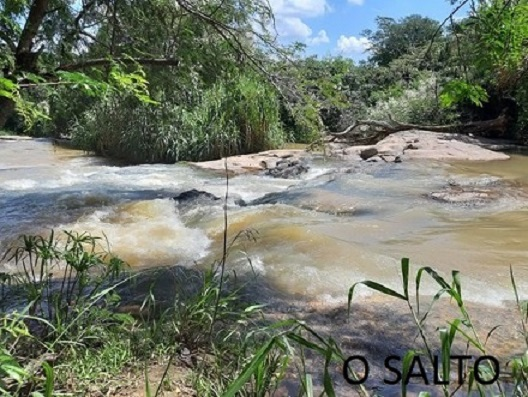
\includegraphics{Imagens/OSALTOB.JPEG}}
\date{Atualizado em 22 de agosto de 2021}

\begin{document}
\maketitle

{
\setcounter{tocdepth}{1}
\tableofcontents
}
\chapter*{-}\label{section}
\addcontentsline{toc}{chapter}{-}

\chapter*{Introdução}\label{introduuxe7uxe3o}
\addcontentsline{toc}{chapter}{Introdução}

Muito bem: não tenho a menor pretensão de arrastar seguidores então vou
escrevendo e mudando de assunto sem preocupação com a ordem cronológica
ou um roteiro estudado ou pré estabelecido. A ideia é fazer apenas um
registro de todas as experiências boas que vivi, assisti ou presenciei.
Como já vivi bastante e pretendo viver muito mais, vou ter muita
história para contar. Em matéria de viver eu quero dar VDO como se dizia
no tempo do fusca que só marcava 120 km/h e depois embaixo estava
escrito VDO que seria 140 ou 150 km/h.\\
Veja que este não é um livro de História no sentido científico da
palavra e, portanto, está sujeito as traições da minha memória. Sinta-se
a vontade para nos comunicar algum deslize ou falha nas nossas
recordações.\\
Então, como dizia o bordão do contador de histórias do Castelo
Rá-tim-bum, na TV Cultura, senta que lá vem história!

\chapter{Os Ourives}\label{os-ourives}

Em primeiro lugar vamos mostrar a casa da Dona Malvina, ou Marvina (em
\emph{saltopiraporês}) para os mais chagados, onde muitos dos
personagens desta história viveram e outros frequentaram.

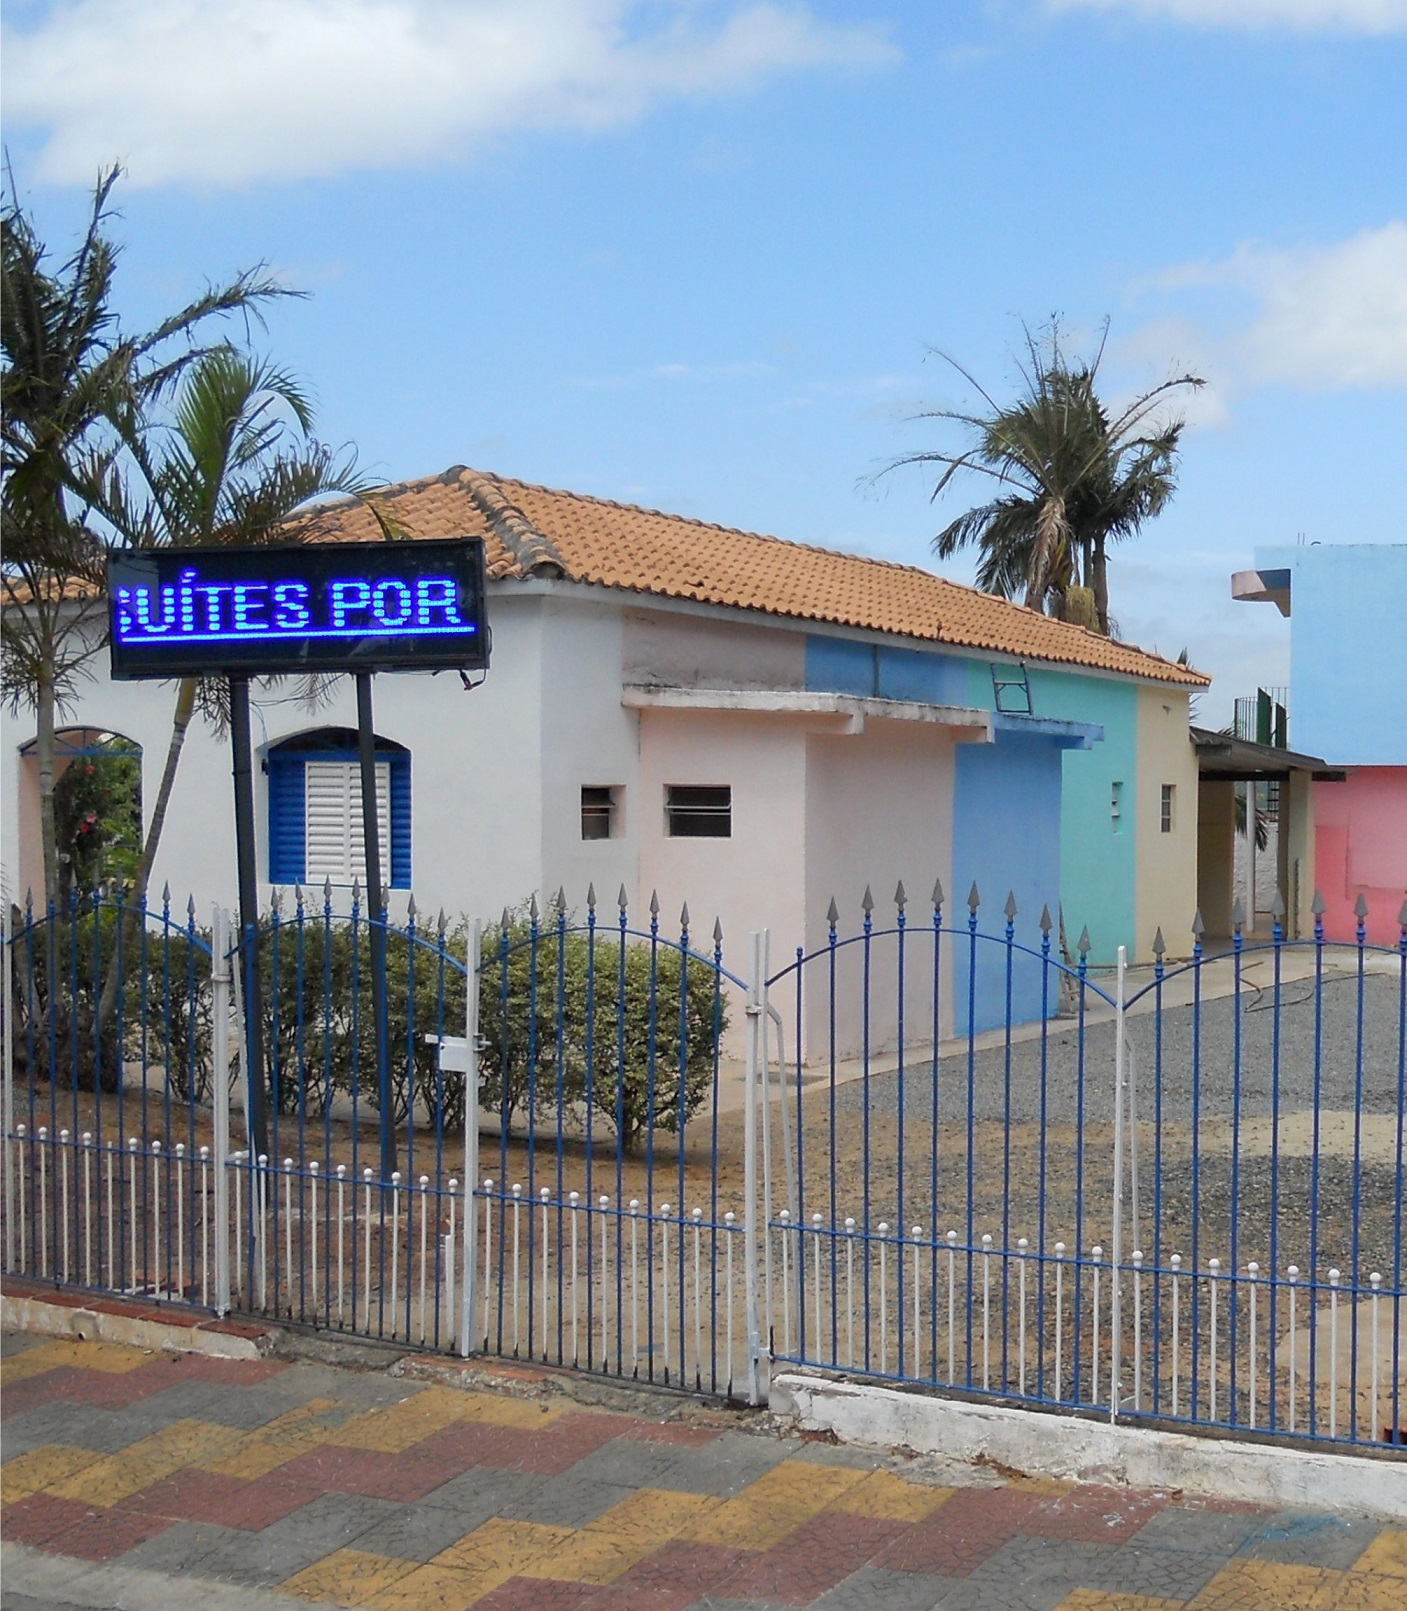
\includegraphics{Imagens/pousada 28.01 metade.jpg}

\textbf{A casa da dona Marvina, que hoje é uma acolhedora pousada}

Como já disse, não sigo um roteiro, nem ordem de qualquer espécie e
conforme os assuntos vão jorrando aos borbotões, vou despejando no papel
sem a mínima preocupação organizacional. Vou continuar assim, misturando
viagens, assuntos profissionais, música e vida pessoal num verdadeiro
``samba do crioulo doido''. Como escrevo sem uma finalidade precípua,
pensando apenas em registrar fatos, mesmo que para poucos leitores se é
que os terei, o mote é jogar para o papel todas essas experiências
fantásticas de vida que tive, tenho e pretendo continuar tendo por muito
tempo, se Deus o quiser. Gosto de dizer que vivo intensamente cada
momento e mesmo nos momentos de explosão de raiva ou decepção, costumo
tirar uma lição de vida e continuar achando que a vida vale a pena. E
muito. Conheci lugares e pessoas fantásticas e com cada uma delas
aprendi um pouco: desde o lavrador analfabeto como o Anselmo que me
ensinou as fases da lua para plantar e para colher, ou o Elpídio Lemes
que me ensinou quando uma vaca estava ``mojando'' até grandes homens de
sucesso como Odilon, Aurimar, seu sócio, Moretti, engenheiro agrônomo
que completou com conhecimentos técnicos o que o Anselmo havia me
ensinado da sua prática de homem simples do campo. O Seu Elpídio Lemes
quando lhe perguntei como saber se uma vaca estava nos dias para
\emph{criar}, ele do alto do seu chapéu de abas largas e do lenço no
pescoço e paletó de brim tentava me explicar: ``Óia Carlinho, quando a
vaca tá mojando, tá pá criá, o vaso dela começa a inchê\ldots{}.'' Eu
perguntei, o vaso sanguíneo Seu Elpídio? e ele: ``Não Carlinho, você óia
por tráis da vaca, no vaso da vaca, ele vai tá inchado''. Ele como homem
de muito respeito não queria pronunciar a palavra \emph{buceta}. Contei
a história para o ``Tonhão Soares'', homem bruto da lida que tinha uma
habilidade extrema com o relho. Quando uma rês tentava se desgarrar do
rebanho, ele do alto do seu baio virava os tentos de couro trançado de
quase dois metros e fazia estalar na orelha do bicho, que murchava e
voltava pro meio do gado. Tinha grande habilidade também para soltar
cabeludos palavrões. Quando contei a história ele repetia em altos
brados: ``Que vaso, que vaso. É \emph{buceta} mêmo,
\emph{buceeeetaaaaa}.'' Aliás Chico Anísio dizia com muita propriedade
que o verbo ``embucetar'' era o melhor verbo que conhecia para descrever
qualquer situação: ``nossa, embucetô tudo, que embocetada do caralho e
por aí vai.'' O Tonhão Soares me contou a história de uma briga do Zilo
c´ô Nésio Diabo. Este já tinha a alcunha porque era o diabo em pessoa. O
Zilo que sabia da fama do outro se defendeu com uma foice. Contava o
Tonhão: ´''Ói, o Zilo deu uma foiçada na cabeça do Nésio Diabo, que roçô
um parmo em quadra''. Ou seja roçou um quadrado de um palmo por um palmo
na cabeça do outro. A expressão ``em quadra'' é muito usada na medição
da ``tarefa'' para arranca de feijão por exemplo. Uma tarefa de chão
dava se não me engano, 22 braças em quadra e a braça era medida do chão
até a ponta do dedo do braço esticado: mais ou menos 2,20 metros. Um
alqueire tem 32 tarefas.\\
Voltando à minha vivência: Conheci muitas mulheres, frequentei muitos
bailes e festas memoráveis. Hoje, maio de 2.020, mesmo neste recesso de
tempos de pandemia levo a minha vida como no filme ``A Vida é Bela'', de
Roberto Begnini. Como se estivesse num jogo de faz de conta, uma
gincana, e a certeza de que tudo vai passar, que o sol vai continuar a
brilhar, a chuva a criar, as flores a desabrochar e a vida a valer a
pena. Por tudo que já vivi me considero um homem bafejado pela sorte.
Sinto a proteção dos meus pais e irmãos que cuidei com carinho extremo e
hoje colho os frutos e me sinto inteiramente recompensado. Tenho uma
vida familiar muito prazerosa e minhas companheiras matrimoniais, tanto
do primeiro casamento como do atual, são pessoas muito dignas, honestas
e competentes e que só me ajudaram e ajudam a fruir e usufruir de uma
vida de muitos pequenos e grandes prazeres. Minha esposa atual,
Patrícia, tem um grande coração e juntos, procuramos ajudar os próximos
da melhor maneira que podemos. Há, especialmente nesse ponto, uma
simbiose total e um propósito de vida em que dividimos o prazer de poder
ajudar à quem quer que seja. Desde um desconhecido que de muletas
precisa de uma carona para chegar na Santa Casa, ou uma pobre mulher que
empurra uma cadeira de rodas ladeira acima para levar a filha jovem
ainda, paralisada por um AVC para um atendimento médico. Uma carona para
uma desconhecida na beira da estrada que espera por um ônibus inter
municipal que não virá devido à uma greve, por ela desconhecida. Tudo
isso nos dá imenso prazer e é maravilhoso dividir com alguém essa
alegria de ajudar o próximo, por mais insignificante que seja essa
ajuda. Me faz lembrar ainda outra história. Estava numa academia de
tênis que fica entre Salto de Pirapora e Sorocaba, onde depois do jogo
fizemos um churrasco e ao tomar a estrada de volta para Salto de
Pirapora me deparei com um carro parado no acostamento. Olhei aquele
carro no meio do nada, faróis apagados e me aproximei com cuidado, sem
descer do carro, temeroso de algum golpe mas vi que dentro do carro
tinha uma mulher com uma criança no colo, sentada no banco do carona.
Baixei o vidro e com certa cautela perguntei o que estava acontecendo.
Ela voltava de Pilar do Sul, o carro pifou e o celular estava
descarregado. Fazia meia hora que estava ali parada, sem saber o que
fazer. Ofereci para levá-la para casa mas ela apenas pediu para usar o
meu celular e chamar o marido, que prontamente atendeu e falou que
estava saindo de casa para vir buscá-las. Ela agradeceu e eu peguei a
estrada para voltar para casa mas, ainda no caminho me arrependi de não
ter esperado com ela a chegada do marido ou então levá-la para a
academia do André, pois a menina sentia frio e a pobre mulher não tinha
um agasalho conveniente: a cobria apenas com sua blusa. Poderia ter
feito melhor mas na hora não me dei conta. Paciência. Numa outra ocasião
notei que uma senhora esperava por horas, perto do portão de uma das
minhas pousadas e não arredava pé dali. Estava esperando por uma carona
que não apareceu e ela morava no bairro da Fazendinha, uns oito
quilômetros de estrada de terra. Avaliei a situação: celular apagado,
sem ônibus, sem parentes para ``pidí pôso'' e ainda começando a chover.
Encarei a estrada barrenta, 16 km ida e volta. Quando estava indo para
Sorocaba, onde já morava com a Patrícia, ela ligou preocupada com a
minha demora. Contei a história e ela de imediato compreendeu a
situação, não levantou nenhuma dúvida e ainda me parabenizou pela
atitude. Mesma situação aconteceu com a Eulália, a primeira mulher. Nós
morávamos em São Paulo e eu vinha para Salto de Pirapora cuidar dos
negócios. Numa dessas vezes, voltando para Sampa no ônibus da Cometa,
sentou-se ao meu lado uma mulher vestida com muita simplicidade, cabelos
compridos ``de crente'' e começou a chorar. Não intervi, deixei que
extravasasse sua tristeza e depois que se recompôs me peguntou se eu não
sabia de alguém, em São Paulo, que precisava de empregada. Contou que
tinha brigado com o marido e abandonado a casa. Descobri que era de
Salto, o pai dela tinha trabalhado para o meu pai e me lembrei de ter
ido à casa dele e visto o filhinho dela que tinha uns 5 anos e tinha os
pezinhos tortos e corria mancando. A mulher, na sua inocência e
desconhecimento da cidade grande, acreditava que chegando na rodoviária
iria perguntando às pessoas e conseguiria um emprego de doméstica. Ainda
me disse que se não conseguisse iria para o Minhocão e conseguiria uma
carona de volta para Salto, pois dinheiro também não tinha mais. Avaliei
os perigos que a inocente mulher iria correr, liguei para a Eulália
falando que iria levar a mulher para casa e ela entendeu perfeitamente a
situação e concordou. A moça dormiu uma noite no nosso apartamento e no
dia seguinte consegui um emprego para ela numa residência em Moema.
Depois soube que ela ficou uma semana e sem aguentar de saudades dos
filhos voltou para o recesso do lar. Soube em Salto que ela sofria de
depressão e tinha tomado a atitude precipitada depois de um
desentendimento com o marido. Fico imaginando essa coitada passando
horas na rodoviária, à mercê dos malandros que vicejam naquela
freguesia. Eu conto essas histórias mais para mostrar a bondade e o
coração das companheiras. Não é para me vangloriar não, posso garantir.

\section{A minha história, do Degas aqui: Carlinhos da
Malvina}\label{a-minha-histuxf3ria-do-degas-aqui-carlinhos-da-malvina}

Vocês devem estranhar o uso quase abusivo da expressão: ``O Degas''
aqui. Mas ela foi usada até por Camões e é a maneira de alguém
referir-se à própria pessoa por exemplo: O Degas aqui é quem manda. Foi
gíria recorrente lá pela década de 60 e denota um certo ar de
superioridade, de ser ``o bom'', de ser ``quem manda ou que tudo sabe''
mas garanto que não é nesse sentido que a utilizo mas sim, pela
lembrança das pessoas que a usavam, se vangloriando e fazendo elogios à
própria pessoa. No popular: \emph{uma metideza} mesmo. Vou contar as
origens da minha família, da minha formação escolar, profissional, mas
não da formação sexual, para não constranger os eventuais leitores.
Kkkkk. Senta que lá vem história.

\section{A saga dos Ourives}\label{a-saga-dos-ourives}

Antes de começar os relatos das histórias quero informar que vou usar
com muita frequência o português coloquial, ou seja como as pessoas
realmente falavam no cotidiano, com erros de ortografia, concordância ou
sintaxe para retratar fielmente a maneira genuína de falar das
pessoas:\\
Este esclarecimento em português coloquial ficaria mais ou menos
``anssim'':\\
``inhante de pincipiá a contá os causo já vô isclareceno que vô usá o
portugueis caipira mêmo, ou mió dizeno: como as pessoa prosiava, do
jeito simpre, sem devorteio''.\\
Você conhece o ``Carlinho do Pedro Orive''? Não? E o ``Carlinho da
Marvina''?. Foi sempre assim que eu fui chamado ou identificado. Assim
mesmo: Carlinho no singular e o Ourives trocado pelo ``Orive'' e Malvina
por ``Marvina'' Qual a razão desses apelidos sempre relacionando meu
nome aos dos meus pais? Era na verdade para distinguir de outros tantos
Carlinhos como o Carlinhos do Elias, Carlinhos do Altino, Carlinhos
Martelo, Carlinhos ``Surdeca'' e outros tantos. E qual a origem do
``Orive''? A família dos meus pais se estabeleceu no bairro antigamente
chamado de ``Purungá'' aqui em Salto de Pirapora, em razão da grande
quantidade de árvores de purungos, também conhecidos como cabaças.
Depois o local começou a ser citado como sítio dos Ourives em razão da
enorme família que herdou a alcunha de Ourives. Tinha o meu pai, o Pedro
Orive, e seus irmãos: o Severino Orive, o João Orive pai do Zequinha
barbeiro que também era conhecido como Zequinha Orive, o Zé Orive além
de duas irmãs: a Dasdores, chamada de ``Dasdor'' pelo meu pai, mãe do Zé
do Santo do armazém onde hoje é a loja SP embalagens e antigamente a
sacaria do Aristide Mandú, e a outra irmã a Inhana do Gênio Bello. E de
onde veio essa alcunha que tanto se disseminou a ponto de dar nome a um
bairro exatamente onde está hoje o condomínio Terras de São Francisco e
de também denominar o córrego dos Ourives que por ali passa? Contavam os
meus pais que um ancestral de quatro gerações anteriores à minha, ou
seja bisavô do meu pai tinha a profissão de ourives. Contavam ainda que
uma sobrinha do papai, a Ditinha do Severino Orive, que era filha do
João Orive ou seja casou-se com o seu legítimo tio tinha um pilãozinho
de ferro com a mão de pilão também de ferro que servia para socar o ouro
que passava pelas mãos do meu tataravô, não se sabe se por ele extraído
ou comercializado.\\
A alcunha atravessou quatro gerações e se manteve até a minha que fui
algumas vezes chamado de Carlinho Orive. Em uma das vezes tive inclusive
meu nome anotado pelo filho do Gustão de Morais, irmão do Izaias, do
Strike e mais uma penca de irmãos da seguinte forma: ``Carlinho
Orrive''. Dei muita risada e perguntei se eu era tão horrível assim. O
rapaz, que cuidava da criação de porcos do Zeca do Fuade, se atrapalhou
todo mas na hora percebi a sua dificuldade para escrever.\\
Eu fui um dos poucos que foi chamado assim porquê vivi e convivi muito
mais tempo com o pessoal de Salto de Pirapora. Já meus irmãos que foram
morar em São Paulo para trabalhar e que ficavam muito pouco em Salto de
Pirapora não eram chamados dessa maneira. Aliás a família era composta
por sete irmãos.

\section{A prole dos Ourives}\label{a-prole-dos-ourives}

O primogênito era o Crizólito e minha mãe se inspirou numa pedra
preciosa de um livro que lia na época e na felicidade com a chegada de
um filho quis lhe dar o nome da tal pedra. A grafia era com ``s'' mas no
cartório foi registrado com ``z''. Coisas do tabelião local que deveria
ser o Chico Pedroso ou seu filho Araldo marido da Dona Norma que herdou
o cartório do marido posteriormente. O Crizólito saiu de Salto com 16
para 17 anos e foi trabalhar em Sorocaba, estudou contabilidade na
Escola de Comércio de Sorocaba(depois OSE) e conseguiu ingressar no
Banco do Brasil, em São Paulo e em São Roque, onde trabalhou até se
aposentar. O outro irmão se chamava Delphino, grafado assim mesmo com
``ph''. De novo o cartorário pseudo professor. Ele também entrou no
Banco do Brasil só saindo de lá quando passou no concurso para fiscal de
rendas do Estado. Depois a Maria que se formou na Escola Industrial de
Sorocaba, hoje Rubens de Farias, que apesar do nome Industrial preparava
moças \emph{casadoiras} para o matrimônio. Ensinava-se até a bordar
monogramas com um aro redondo, de taquara ou madeira, chamado bastidor,
onde se esticava o fino pano de lenço de bolso por exemplo e se
esculpiam lindas iniciais dos noivos, dos recém nascidos ou de quem se
queria homenagear. A saga dos irmãos está relatada individualmente mais
adiante. Depois o Luiz que ficou na lida com o pai: gado e carros de
boi. Dizem que era um moço muito bonito e que se desiludiu com um namoro
com a Carolina que acabou casando-se com o Neguitinho da Transportes
Neguito, filho do Chiquinho Brechó (corruptela de Belchior). O Luiz,
infelizmente, nunca mais teve a saúde perfeita não se sabe se por esse
acontecido ou devido à uma queda do cavalo em que voltou para casa
desacordado em cima do animal ou por outro fator hereditário mesmo.
Depois o Salvador que também foi bancário primeiro naquele que se
transformou no atual banco Itaú. Depois foi também para o Banco do
Brasil, onde se aposentou. Depois o Horácio, grafado assim mesmo com H.
Eita tabelião inventor. Depois conseguiu, com muita dificuldade
burocrática, mudar para Orácio e também não sei porque mudar pois o seu
xará da Grécia Antiga era grafado com ``H'' mesmo. Estudou na escola
agrícola de Pinhal onde também estudou o Nei do Araldo, filho da Dona
Norma, a do cartório de registro civil. Minha mãe dizia que mandou o
Orácio para lá para ver se ``endireitava''. Acabou se tornando bancário
também. No Banespa do Aeroporto de Congonhas em São Paulo.

\section{Seu Pedro Ourives}\label{seu-pedro-ourives}

Batizado, ou melhor com o batistério lavrado Pedro Antunes de Souza
ficou conhecido a vida toda pelo apelido de Pedro Orive e já contamos a
origem da alcunha da família toda. O batistério para quem nunca ouviu
falar era uma espécie de certidão de nascimento emitida pela paróquia
onde a criança era batizada. Daí a origem do nome que também pode
designar a pia batismal onde a criança foi ungida. Documento à época tão
ou mais importante para as famílias cristãs como a certidão de
nascimento. Por coincidência achei ontem o meu batistério lavrado na
Igreja Matriz de Sorocaba. Quando montar o blog vou mostrar. O garoto de
nome Pedro era muito \emph{arteiro} e minha mãe Dona Malvina nos dizia
para não colocar o nome de Pedro nos filhos porquê vinha de Pedro
Malasartes e que então o rebento seria de fazer muitas artes. Meu pai
nasceu e se criou no sítio e foi realmente de aprontar ``poucas e
boas''. Me contou que foi no chiqueiro de porcos da família e, invocado
com os rabos dos porcos que insistiam em fazer uma espiral para cima,
muniu-se de uma faca e cortou os rabinhos dos bichinhos. Imagine a surra
que deve ter tomado. Era muito comilão, muito guloso e as coisas eram
realmente muito difíceis na época. Ele acompanhava o amadurecimento de
um cacho de bananas e quando percebia que ``estava de vez'', ou seja
para iniciar o processo de amadurecimento ele apanhava o cacho, amarrava
na ponta de uma corda, subia numa árvore, passava a corda pelo galho
mais alto e amarrava a outra ponta aqui embaixo, escondida no meio dos
ramos. Quando as bananas estavam maduras, ele soltava a corda, comia o
quanto aguentava e depois içava o resto lá no alto, longe das vistas dos
demais.\\
Depois de casado quando ia a Sorocaba onde o meu tio Raul, irmão da
mamãe tinha um bar na Rua Visconde de Porto Seguro, perto do paredão do
INSS gostava de promover uma brincadeira que adorava. O bar, na região
do clube 28 de setembro ponto de encontro social das famílias negras,
tinha muitos frequentadores da raça. Minha mãe me contou que ele
comprava um barrilzinho de pinga, chamado de corote na época mas nada a
ver com os corotes de agora e chamava os negros para tomar a cachaça e
fazer a brincadeira do ``corvo'' campeiro. Um negro se deitava no meio
da rua como se fosse a ``carniça''. Outro negro saia do bar e ia
verificar se estava no ponto. Batia asas à moda de um corvo ao fazer a
peregrinação. Tudo isso regado a goles de cachaça, num ritual repetido e
constante e aguardente ``indo para o bucho''. Quando o corvo campeiro
dava o sinal verde todos os negros, na espera e consumindo o barril de
pinga, se dirigiam para a comilança, batendo as asas e meu pai se
divertindo e rindo gostosamente do ritual dos negros, imitando os
urubus.\\
Contava que no fim da revolução paulista as tropas voltavam dos campos
de batalha, aos magotes. Um sitiante, zeloso pela hospitalidade, quando
via a \emph{sordadesca} na curva gritava \emph{pá muié}: Cue café Crara
que tá chegando os sordado, judiação. Pouco depois vinha outro grupo e a
história se repetia: Cue café Crara. E outra turma: Cue mais café Crara.
Quando se deu conta que eram muitos batalhões voltando e ao avistar mais
um se aproximando gritou: Num cue mais café Crara: que vão tudo a puta
que pariu.\\
Meu pai quando \emph{imprensava} o dedo numa tábua da mangueira ou num
palanque de cerca dizia que o sangue tava \emph{pisuado}.

\section{A história do início da família do Pedro
Orive}\label{a-histuxf3ria-do-inuxedcio-da-famuxedlia-do-pedro-orive}

Meu pai sempre foi da lida do campo. Amansando bois de carro,
transportou pedra e lenha para as pedreiras em carros de boi ou em
carretas puxadas por bois. Contava que levou cal para Santos num carro
de boi, durando a viagem ``prá mais de meis''. Além do transporte
ganhava dinheiro colocando bois ``chucros'' no carro de bois,
amansando-os para a lida e depois vendendo os mais velhos, já
\emph{mansos de carro} por preços diferenciados. Adquiriu uma bela
propriedade no centro de Salto onde depois foram montados os fornos de
cal do Aníba (Aníbal) de Góes. Como já contei tinha ali um pomar com uma
grande variedade e quantidade de frutas. Depois vendeu essa propriedade
e comprou outra melhor e mais no centro onde implantei os loteamentos
``Recanto Cidade Nova'' e depois o ``Jardim Ilha das Flores''. O Pedro
Orive nessas andanças de carro de boi levando pedra ou cal para Sorocaba
fazia pernoite no bairro do Itanguá, hoje Avenida Luiz Mendes de
Almeida, região do Ceasa Sorocaba, onde meu avô João Batista tinha uma
pequena propriedade de uns 5 mil metros, com um pastinho e uma aguada
boa. Ali acolhia os carreiros, que chegavam, soltavam os bois para
pastar, beber água e pernoitar. Os carreiros estendiam suas esteiras
feitas de taboa (aqueles pés verdes que davam paina, nos banhados),
embaixo dos carros de boi para não ``pegar sereno e não ficarem
constipados''. Cobriam-se com suas capas poncho e ali dormiam. Antes
disso minha avó Dornélia lhes servia uma jantinha que poderia ser uma
canja de galinha ou uma sopa rala de macarrão com feijão e um ``cheiro''
de carne ou um arroz com feijão e ovo frito mesmo. No dia seguinte
``encangavam'' os bois e seguiam viagem levando cal, lenha ou pedra . Os
carros de boi tinham rodas de madeira e emitiam um guincho estridente,
bem característico. Acontece que esse barulho, uma espécie de nhééééééém
prolongado, quase um lamento da madeira!!!!!! um ``canto lamurioso'' foi
proibido por lei municipal, dentro da cidade de Sorocaba. Então eles
carregavam sabão (com certeza de cinza ou de sebo, feitos caseiramente)
e passavam nos eixos dos carros de boi para que estes não ``cantassem''
ao atravessar a cidade. Isto para não serem multados. O maior orgulho de
um ``carreiro'' era o canto do seu carro de boi. Quanto melhor a madeira
mais alto e estridente era o seu canto. Ainda guardo esse som na minha
memória apesar de ter presenciado poucas e inesquecíveis vezes.

Nessas paragens no bairro do Itanguá, no sitiozinho do Vô João Batista e
da Vó Dornélia, o Pedro Orive acabou se encantando com a moça
Marvina(Malvina). Casaram-se e vieram para Salto morar no bairro do
Purungá depois bairro dos Ourives. Minha mãe, moça nova, respeitava e ao
mesmo tempo temia o marido. Como naquele tempo as vendas eram longe e
fora de mão tinha que se virar com a mistura do dia a dia. Meu pai tinha
uma bela criação de galinhas e adorava comer carne de frango. Logo no
início do casamento minha mãe falou: Pedro, o que faço de mistura? Ele
mais que depressa respondeu: Mate um frango e ela o fez. No dia seguinte
a mesma história e ele: Mate um frango e assim foi até que ela falou:
Pedro, acabou frango. Ele então: Mate uma galinha e mais outra e outra.
Pedro, acabou galinha. Ele falou: Mate o galo. Depois minha mãe já
grávida não suportava mais o cheiro de frango, de galinha, de galo.
Depois do parto era costume servir às mães ``de quarentena'' uma canja
de galinha, para restabelecer as forças. Minha avó preparou uma ``bem
gorda'' e levou na cama para minha mãe: Marvina, tome essa canja ``prá
ficar forte e dar bastante leite'' . Minha mãe deu um berro: Suma com
essa canja da minha frente que eu não posso nem sentir o cheiro de
galinha. Me dá até ânsia de ``gômito'' (vômito). Mais para a frente já
com bebê de colo meu pai queria ir no baile. Ela estrilou: Pedro você
não vai no baile sozinho. Ele replicou: Vou no baile sim. Como naquele
tempo os homens não saíam de casa sem chapéu minha mãe pegou o chapéu
dele, trancou no guarda roupa e escondeu a chave no seio. E ele:
Marvina, me dá a chave e ela se negando a entregar. Ele foi no paiol nos
fundos e voltou com um machado: Se você não der a chave eu arrebento a
porta do guarda roupa ``no machado''. Minha mãe teve que liberar a chave
e o chapéu mas pegou o bebê de colo e foi junto no baile. Ficou a noite
toda carregando a criança no colo e ele dançando bem feliz e garboso.
Ela dizia que por isso eu sempre gostei de bailes e de dançar. Meu pai
contava que aprendeu a dançar com um homem. O ``\emph{Paschoar}'' marido
da Mariquinha (mãe da Célia do Zé Martelo) foi quem ensinou meu pai a
dançar. Naquele tempo ninguém se arriscava num salão de baile sem saber
dançar bem. Valia até aprender com outro homem. Bons e inocentes tempos.
Meu pai dizia que para dançar bem ``tinha que pisar na música''. Levei
tempo para entender mas ele queria dizer: acompanhar em cima do compasso
da música.

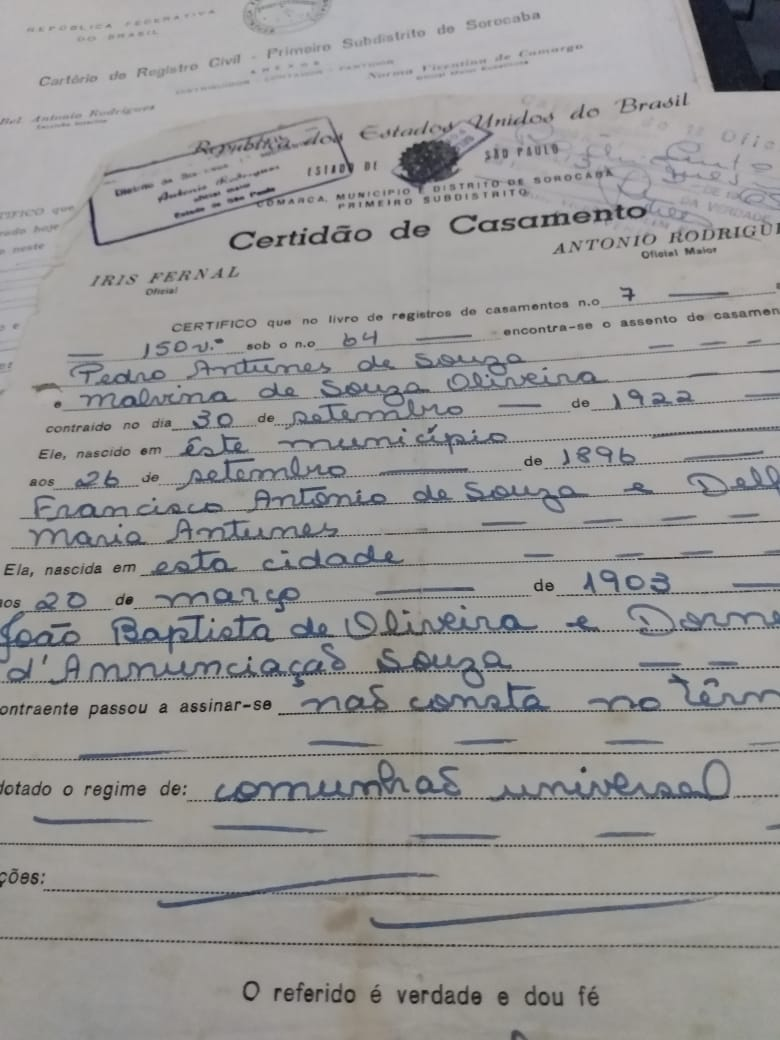
\includegraphics{Imagens/CertidaoCasMalvinaPedro.jpeg}

\textbf{Certidão de casamento de Malvina e Pedro - onde tudo começou}

Meu pai comprou um sítio ``pás banda'' da Fazendinha depois do sítio do
Pedro Belo e depois do João da Nhá Cota. Ali criava garrotes e engordava
para vender ou então para amansar como bois de carro. Teve um discussão
muito engraçada com o vizinho João da Nhá Cota (pai do Balaio) por causa
de uma divisa. Os dois discutiam na grota ao lado do riozinho e o João
da Nhá Cota, que era conhecido como ``pamorde'' porquê tudo que falava
começava com o \emph{pamorde} (com certeza resquício do português
castiço ``por modos quê''). E o Nhô João dizia: Pedro eu ``uósque'' (eu
acho que) a divisa é aqui. Meu pai replicou bravo: Nhô João, uósque num
si escreve, querendo dizer que o uósque não era uma certeza portanto não
deveria ser dito. Fiquei sabendo também depois que meu pai tinha
falecido que ele era mestre na arte de localizar um boi ``alongado''.
Quando um boi ``enraivava'' ele se afastava da manada e se embrenhava no
meio do mato e podia morrer de fome ou de sede pois se recusava a se
alimentar e tomar água. Dizem que meu pai era ``um cachorro'' para
seguir ``o rasto'' do boi alongado. Entrava no mato examinando ramos
quebrados, pisadas do boi até localizar o bicho que era trazido para a
mangueira e tratado ali sozinho até voltar a fazer parte da manada.
Portanto já existia boi com síndrome de pânico e \emph{border line}.
Kkkkk. Nhô João me deixou uma lição. No começo da minha lida eu queria
levar o gado ``na marra'' para a mangueira ``pá lambê sar'' no cocho.
Metíamos os cavalos em cima dos bichos, cercando e tocando para a
mangueira mas eles debandavam e não entravam na mangueira. Nhô João me
disse com toda a calma do mundo: ``Carlinho, você num tem exprência de
lidá cum gado. Eu vô imprestá duas vaca véia que vão madrinhá o seu gado
i insiná os tar pá entrá na manguêra sem atropelo de cavalo i aquela
baita buiarada de pião''. Dito e feito: aprendi a lição do Nhô João.

\subsection{O Carlinho da Marvina}\label{o-carlinho-da-marvina}

Eu, o caçula, a raspa do tacho, o Carlinho da Marvina. Nasci na chácara
onde depois se instalou o Cal São Pedro, do \emph{Aníba de Góis} que
construiu ali alguns fornos de cal de tijolos antigos, grandes e
pesados, um verdadeiro patrimônio da cidade que foi dilapidado mediante
a cegueira do poder público que não soube conservar tão lindos
monumentos que marcaram a saga mineradora da cidade. Vagabundos que por
ali moravam venderam os seus tijolos por uns poucos \emph{milréis}: a
cultura e a tradição de uma cidade formada por pedreiras e fornos de cal
dilapidada por uma ninharia. Mas isso é uma outra história e não adianta
chorar o leite derramado. Pois eu nasci nesse local numa chácara com
tamanha abundância de frutas que minha mãe, a ``Marvina do Pedro Orive''
chegou a fazer vinho (um licor talvez) de mexericas de tanto que as
colhia. Mas o Pedro Orive já tinha comprado uma nova propriedade onde
estão hoje os loteamentos RECANTO CIDADE NOVA e JARDIM ILHA DAS FLORES,
que vim a implantar nas décadas de 70 e 90. Mudamos posteriormente para
a nova casa, na Rua Belarmino, que ainda hoje mantém as antigas linhas
estruturais e onde descobri debaixo de várias camadas de tinta um
resquício da pintura original da casa que destaquei em um pequeno
quadrado que pretendo manter por quanto tempo puder. Lá está e se
suscitar a curiosidade de alguém terei o maior prazer de mostrar. Quando
a família se mudou para esse novo lar, na antiga rua da \emph{Páia} em
frente ao hoje bar do Pupo e perto do sacolão São Sebastião, eu estava
engatinhando e minha mãe me contava que virei uma lata de verniz
inteirinha que estava sendo usada para impermeabilizar o assoalho. Se eu
pudesse teria conservado esse assoalho até hoje: tábuas largas e
compridas de madeira de lei. Assim praticamente nasci e cresci na
``Belarmino''. Era praticamente um sítio dentro da cidade, com cerca de
10 alqueires, com um pomar fantástico formado pelo meu pai. Tinha uns 30
abacateiros, laranjeiras, pereiras, mangueiras, parreiras, pés de
abacaxi e jabuticaba enfim um verdadeiro paraíso frutífero e muitos
moleques ``cataram'' frutas do pomar do Pedro Orive, do que faço piada
sempre que encontro um antigo morador da Belarmino. Peço para ler a mão
e disparo: você roubou manga no `` quintar'' da Dona Marvina. A maioria
acaba concordando que sim. Ali meu pai tinha vacas de leite, cavalos e
éguas para puxar a velha carroça, que lamento não ter conservado e
mantido até hoje junto com os \emph{arriames}: tapa, celote, tiradeiras,
correntes, rabichos, cangas e canzis dos carros de boi etc. etc. Tudo
isso foi roubado por um parente sem vergonha para vender também por
alguns ``mireis''.\\
Fui bom aluno no primário no Grupo Escolar Afonso Vergueiro, mais ou
menos onde era a primeira Prefeitura de Salto, ao lado da farmácia N.
Sra. Aparecida. Sempre fui o primeiro da classe. No meu tempo estudava o
Seme do Zé Turco, o Jaiminho da farmácia, filho do Seu Jaime e da dona
Bibi que fazia maravilhosos lanches na sua casa para que ensinássemos o
Jaiminho a melhorar suas notas. Tinha ainda o Querubim do Zé Fredão que
morava na casa onde está hoje o Serginho Martelo. Eu e o Querubim
disputávamos o primeiro lugar da classe e numa das séries ele conseguiu
empatar comigo. Média 9 para os dois. Fiz o ginásio na Ose e depois no
Estadão em Sorocaba. Este colégio, estadual, era a melhor referência em
escola em Sorocaba, quando o ensino público ainda tinha muita qualidade.
O segundo melhor de Sorocaba era o Municipal, contíguo ao Estadão. Ou
seja, ambos de ensino gratuito superavam os colégios particulares.
Estudar em Sorocaba era uma luta. A estrada de terra intransitável nos
dias de chuva. Cheguei a sair de casa de uniforme branco e voltar
coberto de barro, à pé porquê a \emph{jardinêra} tinha atolado no barro
no subidão do Morro Branco.\\
Depois fui estudar em São Paulo no colégio estadual Fernão Dias Pais em
Pinheiros, também um nicho de excelência em ensino. Mas, caí na gandaia
e fui ``jubilado''. Quando se repetia dois anos seguidos o aluno era
obrigado a deixar o colégio e foi o que aconteceu comigo na terceira
série. Matei muita aula e pulei muito muro no embalo dos amigos e por
gostar da farra também. Moral da história: voltei para Salto de Pirapora
onde só havia primário. Voltei depois para o velho Estadão em Sorocaba
onde concluí o Curso Científico.\\
Trabalhei em São Roque no grupo Carambeí e comecei a fazer a Faculdade
de Matemática. Ia relativamente bem quando a empresa me mandou para São
Paulo para chefiar o Setor de Compras. Mudei para São Paulo e continuei
o curso na Faculdade Tibiriçá no bairro dos Jardins: Alameda Lorena com
Nove de Julho.\\
Novamente a empresa me transferiu de volta para São Roque e voltei para
a Uniso em Sorocaba. Aí sim: bagunçou toda a carga horária e eu já
estava desistindo da faculdade quando o dono da Carambeí Carlos Pereira
Paschoal me convidou para ir para o Paraná trabalhar na parte comercial
de suas fazendas em Céu Azul, região de Cascavel. Consegui lá, longe da
família e da quase noiva formar um pequeno capital. Voltei de lá e me
tornei boiadeiro e plantador de feijão. Fui o primeiro boiadeiro
motorizado que tocava o gado no pasto \emph{muntado} numa moto Honda CG
125. Levava os peões para lida com seus cavalos e voltava para Salto, de
moto, buscar carne, pão e cerveja para fazermos memoráveis churrascos na
beira do rio. O Paulinho Mixirica entrava no mato, tirava dois ganchos,
espetava a carne num galho fino e assava no fogo de troncos secos
juntados por ali . Bons tempos, boas farras. Fui alvo de um sem número
de brincadeiras. O Joel Haddad, o prefeito, encontrando comigo numa
estrada perto do seu sítio no bairro Boa Vista, me vendo na
\emph{motinha} com um laço pendurado na garupa perguntou rindo se eu
estava laçando boi e arrastando na \emph{chincha} na moto. Rimos muito.
Numa outra ocasião precisava ver o gado num sítio distante uma légua (6
km.) de Salto e pedi para o Curiango, da turma das ``lambreta'' arriar a
égua Chita e ir na frente. Dei um tempo e fui de moto. Chegando lá
montei na Chita e o Curiango me falou que ela estava meio preguiçosa.
Para usar espora senão ela refugava. Coloquei as esporas, subi no
animal, vistoriei o gado e \emph{muntei na motinho} para voltar para
Salto. Lá chegando fui abastecer no posto do Walter Benedetti. A
molecada do posto inclusive o Beto Benedetti que deveria ter uns doze
anos mais ou menos, me cercava para fazer brincadeiras. Então um deles
perguntou: ``Carlinho, se num cutucá a motinho na espora ela não anda?''
Só aí me dei conta de que tinha descido da égua e montado na moto com
esporas. No plantio de feijão se dizia: ``menininho'' de escritório se
metendo a plantar feijão? vai quebrá a cara. Felizmente me dei muito bem
nas duas atividades e pude rir gostosamente dos que duvidavam das minhas
empreitadas malucas. Voltei a trabalhar em São Paulo, no mercado de
incorporações imobiliárias, tive estacionamentos no Morumbi e em frente
ao Objetivo da Luis Góes no bairro Vila Mariana . Acabei voltando a
Salto para fazer o loteamento Jardim Ilha das Flores, na área
remanescente do primeiro loteamento Recanto Cidade Nova. Na minha ``lida
de boiadeiro'' colecionei histórias e tipos folclóricos:

\subsection{Crizólito Antunes de
Souza}\label{crizuxf3lito-antunes-de-souza}

O Crizólito foi praticamente o primogênito do casal Pedro e Malvina.
Isso porque os dois mais velhos faleceram cedo e nós os irmãos mais
novos nem os conhecemos. Na verdade os irmãos que convivemos bastante
além do Crizólito foram o Delphino, a Maria, o Luiz, o Salvador, o
Orácio e eu ou seja 7 irmãos de um total de dez. O Adauto cheguei a
conhecer mas estava internado e tinha problemas: era praticamente uma
criança mesmo já bem adulto.\\
O Crizólito nascido em Salto de Pirapora em 1.924 fez os estudos básicos
por aqui mesmo e quando garoto, uns dez anos, a Mamãe já o mandava levar
frutas e quitandas que ela mandava para a nossa avó Dornélia em
Sorocaba, no bairro do Itanguá. A mamãe contava que ele tinha que
carregar uma enorme cesta de taquara e ir de carona na carroceria de um
caminhão levar coisas para a avó pois eles eram muito pobres e tudo que
chegasse era bem vindo. Minha mãe fazia biscoitos de polvilho, bolo de
amendoim, rosquinhas doces, brevidades e enfim um monte de coisas
gostosas assadas no forno de lenha e ela chamava essas guloseimas de
quitandas. Com certeza mandava um frango ou um pedaço de porco abatido
pelo meu pai. Conto isto para mostrar que a coragem da Mamãe em mandar
um garoto em cima de um caminhão para Sorocaba já denotava a sua vontade
de soltar os filhos no mundo. E este fato para o Crizólito já começou a
abrir um novo mundo, além dos parcos horizontes do sítio e da cidade
pequena. Já rapaz o papai botou ele na lida do gado e dos carros de boi.
Ia para os lenheiros carregar lenha que seria enviada para os fornos de
cal. Ou seja, o seu horizonte era virar carreiro de boi e ele começou a
se revoltar com isso. Jogava e adorava futebol e segundo ele mesmo,
jogava muito bem chegando até a ser levado com a equipe de Salto em
Pilar do Sul e outras cidades da região. Contou que fazia lindos gols de
cabeça apesar da baixa estatura e foi apelidado de mamão ou melão (já
não me lembro) por ter a cabeça grande. Mas, na dura lida diária não
conseguia treinar e fazer o que tanto gostava. O Pedro Orive era bom de
prosa e o meu irmão fazia de tudo para terminar o serviço mais cedo, mas
dependia do pai para encerrar a jornada e aí ele engatava um longo causo
com alguém e o Crizólito desesperado para não perder o treino. Não raro
quando desatrelava os bois das cangas já estava escuro e o treino
perdido. Sem treino, não tinha lugar no time. Numa dessas ocasiões,
chegou em casa revoltado, murmurando sozinho: isso não é vida e arrancou
a botina do pé e arremessou sem olhar para onde. Minha mãe quase foi
atingida e quis saber o motivo da ``brabeza''. Ele desabafou que não
aguentava mais aquela vida e a Mamãe, muito corajosa e determinada
encarou o Papai: A partir de amanhã o \emph{minino} não vai mais pro
serviço com você. Vai estudar porquê não nasceu prá ser carreiro de boi
nem um ``caipirudo e chapéuludo'' igual a esse povo daqui. No dia
seguinte ela falou com a mãe e arrumou lugar para o meu irmão ficar em
Sorocaba e dar a importante guinada na sua vidinha desenxabida. De
início foi trabalhar na Prefeitura de Sorocaba como braçal mesmo.
Carregando um caminhão de terra, por ser novo e ter estatura baixa, os
outros operários ao jogar a terra na pá jogavam também na cabeça dele.
Conseguiu então ingressar na Estamparia pois Sorocaba tinha uma vocação
têxtil. Era chamada de Manchester paulista, numa alusão à cidade inglesa
de mesmo nome, importante polo têxtil. Na firma, foi trabalhar no
almoxarifado onde eram descarregados fardos de tecidos e cujas metragens
tinham que ser anotadas por um apontador. E ele carregando fardos na
cabeça e somando mentalmente as metragens. Quando o total ia ser passado
para o romaneio ele gritava: Dá tantos metros. Antes mesmo da conclusão
da soma. Não raro os números não batiam e o apontador revia suas contas
e admitia, sem graça, que tinha errado na soma. O fato de que o rapaz
era muito inteligente chegou aos ouvidos de alguém da administração e
ele foi promovido para o Escritório: já não era mais um braçal. Foi
procurar uma escola para estudar à noite e acabou fazendo Contabilidade
na Escola de Comércio, que se tornaria depois a OSE, Organização
Sorocabana de Ensino, onde também estudei, de propriedade de Arthur
Fonseca Filho, hoje nome de avenida na cidade. A partir daí começou a
procurar concursos e acabou passando no do Banco do Brasil, em primeiro
lugar da cidade de Sorocaba, e aí sim deu o grande salto para mudar
radicalmente da vidinha monótona do interior para a efervescência da
Capital São Paulo. Foi trabalhar no BB agência centro, na Avenida São
João, 33 (minha memória é f\ldots{}\ldots{}. fértil) quase no Vale do
Anhangabaú. Nas ocasiões que estive com ele no Banco ele trabalhava na
CACEX Carteira de Comércio Exterior. Todos os departamentos do banco
tinham siglas de cinco letras: Cacex, Funci, Cassi, e assim por diante.
Foi morar em pensões na Liberdade rua Conselheiro Furtado e Rua Sinimbu
até conseguir comprar uma casa no distante bairro do Caxingui, inóspito
e quase desabitado, uma lonjura. Essa casa fazia parte de um dos
primeiros conjuntos habitacionais financiados por órgãos federais. Era o
Instituto de Previdência do Estado de São Paulo e o bairro ganhou o nome
de Previdência: tinha o Previdência de baixo e sua casa era na Rua
Waldomiro Fleury talvez número 296 (será?????). Esta rua era a primeira
paralela à Avenida Francisco Morato, que acabou se tornando o início da
BR 116, estrada que liga São Paulo a Curitiba. O Previdência de cima
fica depois do córrego Pirajussara e termina nas fraldas da Via Raposo
Tavares, caminho para o Paraná passando por São Roque, Mairinque e
Sorocaba e indo terminar na divisa do estado, na região de Ourinhos. As
casas do bairro eram padronizadas mas ele, que não gostava muito de ser
lugar comum, foi fazendo alterações: colocou grades e muros com pedras,
fez uma boa garagem coberta e dois quartos nos fundos com um banheiro de
serviço. Transformou literalmente a ``casinha de pombo'' numa excelente
moradia, com todo luxo e conforto que a época e a sua situação
financeira permitiam. Visionário, adquiriu um terreno no Jardim Guedala,
praticamente o embrião do bairro do Morumbi, que se tornaria coqueluche
a partir dos anos 60 pois abriga o Palácio do Governo, o Hospital Albert
Einstein além de suntuosos prédios residenciais e comerciais. O Guedala
se tornou um dos bairros mais chiques e exclusivos do complexo Morumbi,
que por se tornar grife, acabou estendendo seu território até as fraldas
de Taboão da Serra e Estrada de Itapecirica. No jargão comercial
qualquer lançamento imobiliário em qualquer ``vivoca'' distante era
anunciado como Morumbi. A aquisição se mostrou um grande negócio e a sua
venda com certeza serviu para alavancar investimentos importantes de
seus filhos. O Crizólito se casou com a Mariana Pagano, chamada na
intimidade de Nina, de uma família da Vila Madalena, um bairro hoje
considerado \emph{cult} de São Paulo. Fixaram residência na casa do
Previdência e ali vieram os filhos: Carlos Eduardo, Maria Cecília e
Célio. Tempos depois ele se transferiu para São Roque, talvez visando
uma cidade mais pacata para criar os filhos e fugir da loucura em que já
estava se transformando a Pauliceia Desvairada. Morou inicialmente em um
apartamento e logo construiu uma bela casa com dois pisos na rua Américo
Margonari (número 95?????) bem no centro e perto do banco. O Carlos
Eduardo foi estudar no Bernardino de Campos, que ele chamava de ``berne
ardido do campo'', um colégio estadual e ele sempre foi o primeiro da
classe, ganhando todos os anos um cheque da Prefeitura como prêmio pelo
seu bom desempenho. A Cecília e o Célio estudaram no Manley Lane. O Cá
foi fazer cursinho em São Paulo. Talvez no Anglo, no bairro do Paraíso e
entrou para a sonhada USP onde cursou e se graduou em Engenharia, não
sei a especialidade. Tentou um emprego em Santa Catarina mas a distância
frustrou os planos. Fez concurso para o Banco do Brasil, imitando os
passos do pai, passou e assumiu mas não gostava da rotina burocrática do
banco e acabou saindo. Prestou outro concurso para a Caixa Econômica,
onde acabou se aposentando.\\
A Cecília, chamada de Cecilinha na família, deve ter se formado
igualmente pela USP e o Célio na Mackenzie. Me confirmem por favor. O
Célio trabalhou numa empresa chamada Microtec no bairro do Caxingui,
então uma pioneira no ramo da informática e acabou vislumbrando um nicho
de mercado totalmente novo e ainda embrionário. Abriu uma pequena
empresa com o nome de Impacta que foi crescendo e se transformando em
referência no mercado de TI (Tecnologia da Informática) focando o
segmento de softwares, desenvolvendo treinamentos e hoje com uma
Universidade de Informática atingiu a impressionante marca de 1,5 milhão
de pessoas que se qualificaram por intermédio dos cursos ali
ministrados. A Cecília depois de algumas experiências em empresas como o
grupo Zogbi, passou a integrar o quadro societário da Impacta, com sede
na Avenida Paulista, onde ocupa cinco andares inteiros. A Universidade
fica no bairro da Barra Funda mas ele precisa me fornecer mais detalhes:
número de alunos, tipos de cursos etc.\\
O resumo, ou seja a visão geral da vida do meu irmão mais velho se
resume à uma história de muito sucesso profissional, financeiro e também
comercial. Ainda nos tempos de solteiro montou um Cursinho Preparatório
destinado a preparar alunos para ingressar no Banco do Brasil ou outras
instituições que só admitiam concursados. Ministrava ali aulas de
Matemática com grande competência pois a aptidão com números mostrada lá
atrás na Estamparia, se ampliou mais ainda na resolução de intrincados
problemas matemáticos que poderiam ``cair'' nas provas do temido
Concurso do Banco do Brasil. Os outros professores que conheci, pois
também trabalhei um pouco na recepção do que ele chamava de Cursinho
foram o Delphino meu irmão e o José Brandi Ribeiro, o Brandi, figura
folclórica de quem falaremos depois mas ambos muito inteligentes também.
Eu não sei em que época o meu irmão se desfez do Cursinho mas deve ter
sido quando resolveu mudar seu domicílio para São Roque. Na cidade
começou a jogar tênis e foi um dos precursores do esporte na cidade. Ou
seja, praticamente o tênis nasceu com ele na cidade. Começou a ministrar
aulas e muitos dos jogadores da cidade com certa proeminência na região
como Carlos Aurélio, o Paschoal e o Adriano deram suas primeiras
``raquetadas'' sob a batuta do meu irmão no São Roque Clube e depois no
Raquete Clube, do Olavinho, já no bairro do Taboão, na Estrada do Vinho.
Depois veio o empreendimento imobiliário em Salto de Pirapora, o
loteamento Recanto Cidade Nova, cujo nome é de autoria dele. Num terreno
da família, fizemos praticamente sozinhos e com muita oposição de alguns
irmãos, a implantação do loteamento, que é hoje considerado o melhor
bairro da cidade de Salto de Pirapora. Essa realização foi uma
verdadeira ``briga de foice'' pois alguns dos irmãos contestavam a nossa
liderança e de uma certa forma até desconfiavam dos nossos propósitos
quando na verdade o que queríamos era viabilizar o empreendimento e como
o terreno estava no nome dos sete irmãos tivemos que fazer verdadeiras
peregrinações para colher assinaturas: São Bernardo atrás do Delphino,
que sempre foi refratário ao empreendimento por entender que as suas
idéias mirabolantes não eram acatadas. Alfenas em Minas Gerais para
colher assinaturas da Maria e do marido Paulo, este numa postura
pretensamente desinteressada mas nada receptiva. Mandava que a Maria
assinasse os documentos sem ler pois de qualquer forma teriam que
cumprir o que nós estávamos determinando. O Orácio, que por ter sido
``apeado'' da liderança, discordava e dificultava todas as nossas ações,
que diga-se de passagem sem remuneração alguma por gastos de
deslocamentos e até mesmo pequenas despesas como cópias autenticadas,
taxas de cartório e etc. O Salvador foi o único que colaborou, até com
entusiasmo, na nossa dura empreitada. O Orácio, formado agrimensor,
iniciou o processo junto à Prefeitura de Salto de Pirapora e começou a
trabalhar no projeto propriamente dito mas, apesar de afirmar que
``varava'' noites trabalhando, a coisa não andava. Passados dezoito
meses mais ou menos tivemos que dar um ``golpe branco'', para retirá-lo
do comando e descobrimos que o projeto geométrico tinha falhas
gritantes. Contratamos outro agrimensor que fez o serviço em pouco mais
de 40 dias e uma empresa para fazer aprovação do loteamento: a Renê
Regularizações, da Rua Margarida na Pompéia. O Renê era um conhecido do
Salvador. Resumo da ópera: o que o Orácio não conseguiu em dois anos nós
conseguimos em 90 dias.\\
Aprovado o loteamento veio outro ``parto de ouriço'': a divisão dos bens
e novamente o Orácio impondo e exigindo até o ponto que eu disse à ele
que ficasse com tudo sozinho que era o que parecia estar querendo. Para
chegar a um consenso o Delphino teve que trocar o quinhão dele pelo do
Orácio, o que foi péssimo negócio para ele Delphino, por razões que não
vale aqui mencionar. Acertada a divisão que foi registrada em ata e tudo
o mais na hora da outorga mútua das escrituras novamente o Orácio
``empaca a mulinha teimosa''. Tivemos que dar à ele mais dois terrenos
para que ele concordasse em ir ao Cartório dar sua anuência, sem a qual
nada poderia ser feito pois todos estavam amarrados entre si como sete
irmãos xifópagos. Depois da divisão e respectiva escritura os fatos
tomaram rumos diversos, ocorreram dissensões mas o resumo final é que se
não fosse o nosso empenho conjunto o empreendimento poderia até sair mas
com um grande atraso e com grosseiros erros do projeto.\\
Acontece que a viabilização do projeto e a posterior venda desses
imóveis principalmente a parte do Luiz era crucial para a sua
subsistência. O Papai e a Mamãe precisavam de muito pouco para viver:
graças a Deus tiveram boa saúde e nunca se fez necessária uma
intervenção cirúrgica ou extrapolando uma internação numa UTI. Quanto ao
Luiz, passou a se sentir mais confiante por não mais depender da
caridade de alguns irmãos pois passou a ter o seu próprio dinheiro e com
a administração dos seus proventos pudemos dar a ele condições mais
dignas de sobrevivência, terminando seus dias na Clínica de Repouso Elo,
em Atibaia onde foi carinhosamente cuidado por enfermeiras bondosas que
lhe davam até a comida na boca.\\
A ida para São Paulo do Crizólito e o seu sucesso na sua empreitada
foram cruciais para o rumo das vidas dos demais irmãos, que agora tinham
na Capital um ponto de apoio. Um a um foram se transferindo para São
Paulo e todos, exceto o Luiz, moraram por algum tempo na casa dele até
estabelecer o rumo definitivo de suas vidas. Eu fui levado pelo meu
irmão, por insistência dele pois a Mamãe não queria que eu deixasse os
estudos em Sorocaba. Como ela foi visionária e tinha razão. Fui para São
Paulo mas a empreitada não se mostrou uma boa escolha e tive que
retornar e retomar os estudos por aqui, o que ocasionou um atraso de
alguns anos na minha formação, que aliás acabei não concluindo por
motivos profissionais. Fui trabalhar na região de Cascavel no Paraná e
acabei abandonando a Faculdade de Matemática. Tanto a minha frustração
na época por não ter entrado também para o Banco do Brasil quanto a
interrupção da faculdade não me fizeram nenhuma falta. Na primeira
hipótese seria um burocrático bancário e além do mais o Banco do Brasil
foi muito bom na época do Crizólito e do Delphino. Antes de existir
décimo terceiro salário eles recebiam 15 salários no ano: os doze
mensais e mais três de gratificação. Prestei o concurso e obtive
colocação número 180 num total de 6.000 candidatos mas fui reprovado no
Psicotécnico, um teste a meu ver totalmente subjetivo, com critérios
para lá de duvidosos. Ainda sobre o BB na época o Crizólito tinha a
chance de fazer serviços extras para o próprio banco. Chegou a carregar
malas com numerário (dinheiro em espécie) para levar em cidades
distantes como Assis por exemplo e o Banco remunerava bem esse trabalho.
Iam em dupla, de trem, viajando a noite inteira com malas ``socadas'' de
dinheiro e um revólver no bolso. Acredito que tinham que se revezar para
dormir, para não haver descuido. Imaginem essa situação hoje. Eu também
por volta de 1.980 saía sozinho do Banco do Brasil em Cascavel com duas
maletas recheadas de dinheiro que era sacado na tesouraria para não dar
na vista. Entrava no Opala vermelho, que tinha sido do Crizólito, e me
mandava para a fazenda do Carlos Paschoal para fazer a remessa por
pequenos aviões com destino a Assunção no Paraguay, para fazer câmbio em
condições mais favoráveis. Um baita risco porquê além de assaltos a
operação se constituía em saída ilegal de divisas. Tudo para ganhar uns
míseros trocados na operação cambial. Mas como recebia ordens tinha que
cumprir e a lei era ``bom cabrito não berra''.\\
Como prometi vou falar do Brandi, professor do Cursinho do Crizólito.
Era um sujeito sistemático e pragmático e falava e sonhava com fervor
quase revolucionário. Tinha uma prole imensa para prover e vivia pedindo
grana emprestada para o Crizólito. Sua mulher era a Terezinha, mulher de
modos e silhueta finos. Uma \emph{Lady} educada e atenciosa e o marido
com seus cabelos desgrenhados, óculos maiores que o rosto, sempre
sonhando com projetos megalomaníacos. Sempre levou uma vida sonhadora
mas não era objetivo nem prático como o Crizólito. Na verdade me ocorreu
agora que foi ele que fundou o Cursinho e o meu irmão foi dar aulas como
professor contratado dele, e como sempre tinha reservas guardadas na
``burra'', começou a emprestar dinheiro para o Brandi, passando a
financiar o seu negócio até adquirir o controle invertendo então os
papéis: o Brandi que passou a ser professor remunerado por ele. Morava
no Conjunto dos Bancários na Vila Mariana, já perto da Avenida Klabin e
vivia com prestações atrasadas do imóvel, sempre numa situação
financeira periclitante. Já o Crizólito economizava tostões e eu e o
Carlos Eduardo o chamávamos de Tio Patinhas, e ele gostava. Me lembro
que morando no Previdência, havia duas opções para comprar o leite
diário, que vinha num litro branco de boca larga. Sonho até hoje
encontrar esses vasilhames pois coleciono objetos antigos. A primeira
opção no início da ``subidona'' da Francisco Morato e a segunda no topo
da dita subida já quase no largo do Caxingui. Nesta o leite custava 3
centavos mais barato (não sei qual era a moeda, cruzeiros talvez) e
claro que eu tinha que enfrentar a árdua subida para comprar o leite
mais barato. Todos os dias. Ainda me lembro dos vizinhos do Jardim
Previdência. Na esquina a Sizina Cecatto, na frente um senhorzinho de
bigode que o Crizólito apelidou de ``fiscal de rua'' pois o dito cujo
vivia bisbilhotando a rua o dia inteiro. Tinha uma filha linda, a
Raquel, por quem o Delphino era apaixonado, mas sem a devida
correspondência. Mais abaixo vinha o Tomithão, policial com cara de
bravo mas mesmo assim namorei a Aimar filha dele e irmã do Hamilton que
tem a Tomithão Veículos na Avenida Pirajussara, perto do Shopping
Butantan. Ainda tinham os gêmeos se não me engano Ricardo e Roberto.
Moravam quase em frente. No início da Waldomiro Fleury tinha uma capela
onde frequentei muitas missas dominicais suspirando pelas meninas
bonitas que nos ignoravam por completo. Atrás da igreja tinha um
campinho de futebol onde ``estourei'' o menisco do joelho direito e
nunca mais pude jogar futebol direito. O esporte perdeu um grande
craque. Kkkkkk. Ao lado do campo tinha a chácara do Cristhie, famoso por
dar tiros de sal na bunda dos moleques que pulavam seu muro para roubar
frutas. Cheguei a sair do Previdência de bicicleta e fomos ao Embu das
Artes buscar água com um garrafão toscamente preso na garupa por um
elástico. Sem farol, apenas com a camisa aberta achando que isso era
suficiente para os carros nos verem. Que loucura.\\
O Crizólito era chamado de Crizo pelo Carlos e de paizinho pela Cecília.
Mas quando dava aulas de tênis gostava de ser chamado de Mister Criz,
creio que numa alusão ao Mr.~Frank, que junto com a esposa Dona Ruth
plantou a semente do tênis em Sorocaba.\\
O meu irmão à exemplo do Pedro Orive era bom de garfo. Quando solteiro
vinha passar o Natal em Salto de Pirapora. O Papai normalmente matava um
porco e à pedido da mamãe um cabrito, sem contar com a leitoa assada no
forno da padaria. O Crizólito queria comer viradinho dos miúdos do
porco, torresmo, lombo frito ou assado e ainda saia com o papai à cata
de alguma roça de milho verde para a mamãe fazer pamonha. Fazia uma
mistureba e não raro passava mal pois não continha a gula. Na verdade
quando vinha de São Paulo queria matar as saudades dessas comidas todas
e numa ânsia desenfreada queria comer de tudo e ao mesmo tempo. Com
relação a bebidas os amigos dele de São Roque falavam que ele era ``ruim
de mistura'' pois queria tomar caipirinha, cerveja, uísque e o que mais
viesse à frente. Mas sempre foi um bebedor social, aproveitando as
ocasiões de jantares dos amigos de São Roque ou festas para tirar o
atraso porquê no dia a dia em casa raramente bebia alguma coisa. Também
não era frequentador contumaz de bares, ao contrário dos seus colegas de
banco e do Zomo dentista, este sim um bebedor inveterado.\\
Fizemos várias viagens juntos, principalmente ao Paraná, quando eu
trabalhava em Céu Azul e numa das vezes fomos até Assunção. Nessas
viagens conversávamos muito e tínhamos uma boa sintonia para comer,
beber e passear. Em Assunção ficou hospedado comigo no hotel Guarany, um
dos melhores à época e como eu tinha tudo pago pela empresa, o incluí no
pacote da hospedagem. Ele parecia um marajá se deliciando com as
excelentes acomodações do hotel, ``la noche paraguaja'' e aproveitou
muito as mordomias que pude lhe proporcionar, custeadas pela empresa. No
dia da viagem de volta, por volta das 10:30hs da manhã ele com as malas
arrumadas abriu uma cerveja na suíte e eu estranhei pois tínhamos tomado
o ``desayuno'' há pouco tempo. Ele falou que ia tomar porquê senão ia
perder, como se não soubesse que o consumo do frigobar entraria na conta
depois. Outra história sua de hotel foi quando viajou para uma estação
de águas e levou um creme de barbear do tipo Noxzema que a Cecilia havia
lhe dado de presente para a viagem. Ele nunca tinha usado e se aproximou
do espelho do quarto e acionou o spray com toda força espalhando espuma
de barba pelo quarto todo. Isso foi ele que me contou, rindo muito.
Fizemos muitos churrascos em Salto quando íamos juntos resolver questões
da aprovação do loteamento e ele adorava quando eu assava uns bifões de
alcatra no sal grosso. Eu encomendava a carne com 3 dedos de espessura e
fazia só no sal grosso, bem no estilo ``boi berrando''. Ele se derramava
em elogios e atacava freneticamente os bifões. Adorava disputar partidas
de tênis apostando alguma coisa e se gabava de ter crédito de vinte e
tantas garrafas de vinho, ganhas no tênis, com o Jorge, um parceiro
constante que trabalhava em uma empresa de filtros dosadores em São
Paulo.\\
Tinha muita amizade com o Zomo dentista mas esse era um cara sem muitos
escrúpulos. Ele inclusive me contou que uma extração de um dente da
Cecília poderia ser evitada mas o mercantilismo do amigo dentista o fez
aceitar uma cirurgia, que se constatou depois, ser totalmente
desnecessária. O Zomo quando com grau etílico elevado, fazia xixi no
vaso de plantas da casa onde tinha sido convidado para beber e comer e
outras baixarias do gênero.\\
Outras amizades eram o Renato de São Paulo, que comercializava jóias de
ouro e tinha também o Eros, vegetariano empedernido e cuja amizade
parece que já vinha de São Paulo. Coincidência ou não, seus amigos
incluindo o famoso Brandi tinham belas mulheres.\\
Tinha uma turma boa de copo no tênis e ele convidou alguns para tomar
uísque na sua casa e tinha um cara que a cada nova dose da bebida
falava: ``Tá um mel seu Crizo'' e foi mamando o mel até ver o fim da
garrafa. Nunca mais levou ninguém dos aproveitadores de São Roque para
beber na sua casa. Ainda vou me lembrar o nome desse cara. Em São Roque
tinha uma vizinha ciumenta e esperta que vinha todo dia pedir para usar
o telefone dizendo que ia fazer uma ligaçãozinha ou duas mas, um dia ele
espiou o rascunho com os números anotados e descobriu que eram
interurbanos mesmo.\\
Quando morei em São Roque saíamos no final da tarde para comer alguma
coisa fora e um dos points era o gostoso ``Bio´s Bar'' ao lado da
Matriz. Fazia bons lanches à exemplo do Bio´s lanche e também porções.
Um dia pedimos uma porção de frango frito acompanhada de arroz e fomos
comendo até que sobrou apenas uma única sobrecoxa de frango e começaram
os salamaleques: pega você Crizólito. Não pode pegar você e assim por
diante. Numa certa altura ele se virou para mim e falou: Pode pegar a
última porquê eu tenho uma coxa escondida aqui no meio do arroz e
descobriu a coxa gorda, intacta, que ele tinha reservado antecipadamente
para qualquer eventualidade. Íamos muito no Baú e no Cantinho, um
barzinho escondido quase em frente ao Baú. Também íamos no festival de
alcachofras em um restaurante perto do Stéfano e me lembro da
``alcachofra à la infierno'', com as pontas das folhas cortadas e
recheadas de carne moída mas o que ele mais alardeava e falava que iria
me levar um dia era o bacalhau na brasa da festa do vinho. Segundo sua
descrição, pois nunca tive o prazer de ir, era uma posta alta de
bacalhau assada na brasa com alho e generosamente regada com azeite. No
Stéfano, na altura do km. 58 da Raposo, a especialidade era o canelone,
famoso até em São Paulo. O restaurante existe até hoje, no meio de um
bosque e lá estive há uns três anos com a Patrícia: servem uma sequência
de pratos que começa com uma salada verde que tem inclusive flores
comestíveis, mudas trazidas pelo simpático Estéfano (já falecido) da
Itália. Depois vem uns embutidos e na sequência canelone, frango assado
atropelado, aberto ao meio e crocante, spaghetti, coelho assado e enfim
um rodízio digno da cozinha da \emph{mamma} que era comandada por sua
esposa e agora pela filha Daniela, cujos filhos eram alunos de tênis do
Crizólito.

\subsection{Delphino Antunes de Souza}\label{delphino-antunes-de-souza}

Era o terceiro na ordem decrescente e seguiu os passos do irmão mais
velho prestando concurso para o BB e indo também trabalhar na matriz da
Avenida São João. Era do tipo sonhador e bastante desleixado em todos os
sentidos principalmente na parte financeira. Distraído, tomava o bonde
lotado e não raro tinha o relógio de pulso roubado e só percebia depois
que já tinha descido. Não usava carteira e tinha dinheiro em todos os
bolsos da calça e do paletó. Ia pagar a passagem e retirava uma nota
graúda, pegava o troco e socava num bolso e se esquecia. Na próxima
despesa tirava outra nota graúda e enfiava o troco em outro bolso.
Quando se lembrava que tinha trocados em um bolso, enfiava a mão sem
olhar e não rara derrubava notas pelo chão. A mamãe quando ficou um
tempo na casa dele no Jardim Monte Alegre, depois do Taboão da Serra
separou duas latas de leite Ninho das grandes e numa recolhia todos os
trocados que achava perdidos em bolsos de roupas postas para lavar ou
mesmo caídos pelo chão e quando o Delphino dizia que estava sem dinheiro
ela ia buscar na tal lata e contava que o dinheiro era dele mesmo,
perdido pela casa. Na outra lata foi juntando bitucas e mesmo cigarros
quase inteiros que ele largava pela casa. Não raro acendia um, esquecia
e logo depois acendia outro. A ideia dela era mostrar o quanto ele
fumava, exibindo a lata cheia depois de alguns dias. Mas de nada
adiantou o seu esforço disciplinador. Ele continuava o mesmo. Eu digo
que era do tipo sonhador por conta de certas histórias e uma delas foi o
Crizólito que me contou. Ele trabalhava no setor de ordens de pagamento,
a ORPAG, sigla do banco sempre com cinco letras. Acontece que muitas
dessas ordens não eram reclamadas pelos destinatários por motivos
diversos e ele, com um coração de ouro, anotava os endereços dos
favorecidos e ia nos fins de semana, às suas expensas, a longínquos
bairros procurar as pessoas pois entendia que elas estariam precisando
daquele dinheiro e talvez nem tivessem conhecimento do crédito.\\
Era muito inteligente mas sistemático: quando me deu aulas de Latim, me
fez começar pelo prefácio do livro, e eu impaciente queria ir logo para
as matérias propriamente ditas. Minha mãe falava que ele era muito
afobado e realmente o era. Quando meu pai se decidiu por fazer o
primeiro loteamento ele já foi para o quintal , pegou uma escada e
começou a destelhar uma privada que ainda estava em uso. Nem o projeto
havia sido feito e ele já saiu removendo obstáculos para o futuro
empreendimento. Falava que o loteamento tinha que ter uma avenida de 30
metros como via principal, pois um dia a cidade iria crescer e essa
seria a mais importante via da cidade. Mesmo hoje, mais de cinquenta
anos depois, os loteamentos que fizemos não comportam uma avenida desse
porte. No outro extremo o Orácio com planos de fazer uma avenida
passando bem no local da residência. Pergunto onde a família iria morar
se ele levasse a empreitada a cabo. Finalmente se decidiu fazer uma rua
de entrada desviando da casa e até da jaqueira que existia no quintal.
Isso resultou numa rua em curva e pelo meu aprendizado posterior as ruas
devem ser retas para otimizar o percentual de aproveitamento da área e
devem ser na largura mínima exigida pelas leis municipais, pois exceder
essa largura significa diminuir áreas dos lotes, ou seja menos lotes
menos faturamento. Estes fatos explicam porquê era refratário às ideias
minhas e às do Crizólito. O Delphino não tinha tino comercial e quando
quis adquirir um imóvel, as escolhas que fez e pediu a opinião do
Crizólito este as reprovou todas e o aconselhou a continuar procurando.
O Delphino, em seus desvarios, achava que o irmão tinha ciúmes dele e
colocava defeitos para que ele nunca comprasse um imóvel. Foi então que
comprou a tal casa no Jardim Monte Alegre, uns 3 km. depois do centro do
Taboão. Um local mal servido por ônibus e sem iluminação pública na via
de acesso ao bairro. Quantas vezes, quando morei com ele, descemos no
largo do Taboão e caminhamos por quase uma hora, em plena escuridão para
chegar em casa porquê havia poucos horários de ônibus.\\
Ele se meteu na política em Taboão da Serra e fazendo uma campanha por
uma tarifa única dos ônibus conseguiu se eleger. Os ônibus para o bairro
eram intermunicipais e portanto mais caros. Assumiu a vaga bem no calor
da Revolução de 1.964 quando Adhemar de Barros, demagogicamente,
organizava as Marchas com Deus pela Liberdade, fustigando o governo
Jango Goulart que já claudicava e foi derrubado em 31 de março daquele
ano. Já com os militares no poder o Delphino fez virulentos discursos na
Câmara contra a prefeita Laurita Ortega, que se alinhava com o governo
do Estado(Laudo Natel?) e, portanto da direita na época. Jango Goulart
era esquerdista e parecia querer implantar o comunismo no país, o que
motivou a revolução e o seu respectivo exílio. Ou seja, fazer um
discurso público defendendo essa ala perdedora e perdida nos objetivos
era de alto risco na época. Teve sorte que ninguém deu bola para os seus
discursos e nunca foi ameaçado por isso. Porquê começava no país a época
dos anos de chumbo, com gente ``desaparecida'' como Rubens Paiva e
caçados como Marighela, morto dentro de seu fusca, completamente cercado
pela polícia e desarmado.\\
Prestou concurso para Fiscal de Rendas do Estado e foi aprovado,
assumindo em São Bernardo do Campo e lá adquirindo uma casa, na Rua
Américo Margonari. Por ser muito honesto nunca aceitou participar das
panelas e conchavos com fins obscuros. Esse fato, provavelmente o tornou
um ``estorvo'' para o ``modus operandi'' dos servidores e acabou sendo
transferido para São Paulo, no bairro do Ipiranga. Ou seja, quando
estabeleceu domicílio na mesma cidade em que trabalhava foi transferido.
Adquiriu uma casa na Travessa Humberto Primo no Paraíso, perto da
Rodrigues Alves e do metrô Ana Rosa e depois de fincar raízes com a
família, foi novamente transferido. Para onde? De volta para São
Bernardo. Ele nunca citou essas perseguições e isso foi conclusão minha
mas, era muito estranho ser sempre jogado para longe do local de
moradia. Ganhava muito bem pois os fiscais eram remunerados pela
produção, ou seja pelas multas aplicadas mas, totalmente desorganizado
em suas finanças vivia sempre em apuros. Recebia no início do mês e como
sabia que o dinheiro iria faltar antes do próximo pagamento, reservava
uma quantia e pedia para o Salvador guardar para ele e devolver na hora
do aperto, da dor de barriga financeira. Ganhou três carros zero
quilômetro num sorteio de uma grande loja de departamentos, mas os
vendeu rapidamente e nunca teve um carro novo e em bom estado.\\
Outra característica sua era escrever longas cartas aos irmãos com
críticas ou acusações estapafúrdias ou lições de vida e de moral. Eu
odiava quando as recebia e tinham uma particularidade marcante: a sua
máquina de escrever tinha uma falha na tecla ``tê'' e as palavras com
essa letra ficavam mancas: tinha que adivinhar o sentido delas. Hilário
demais.\\
Chegou a dar conselhos para o papai dizendo: Cuidado, o dinheiro escorre
pelos vãos dos dedos. Que ironia: o papai sempre econômico, adquirindo
boas propriedades, gado e até casas de aluguel que construiu na Rua
Belarmino com tijolos feitos no seu próprio olaria, que ficava na atual
área verde do loteamento Jardim Ilha das Flores, que incorporei. Justo
ele que esbanjava, perdia e aplicava mal o seu dinheiro queria dar
conselhos ao pai. No fundo, era um medo infundado com relação a mim pois
nessa época eu já começava a administrar os bens da família, ajudando o
papai que já não podia mais montar a cavalo e começava a passar o bastão
para mim. Cheguei a ter procuração com plenos poderes para vender as
propriedades mas nunca usei e não usaria sem o consentimento dos pais.\\
Numa certa altura da vida, meu pai muito previdente resolveu passar as
propriedades para os filhos, para evitar despesas de inventário. Até
nisso tinha uma excelente visão, apesar de nem ao menos assinar o nome.
Me incumbiu dessa tarefa e me lembro até hoje quando fomos ao Cartório
em Sorocaba e o Oficial Maior dizendo à ele: seu Pedro, não faça isso.
Na minha vida de cartório vi muitas famílias que foram morar na rua,
despejadas por filhos e cônjuges interesseiros, depois de se apossarem
das propriedades. Contou uma história que muito me marcou e
impressionou. Um casal resolveu dividir a propriedade em vida destinando
um quinhão a cada um deles e para o filho solteiro que morava com eles
deixou a parte da casa em que moravam porquê achavam que ali
continuariam. Acontece que o filho se casou, trouxe a mulher para a casa
dos pais e ela começou a implicar: Não aguento mais esses velhos na
nossa casa e eles foram simplesmente para o ``olho da rua''. História
real, porém muito parecida com a triste moda de viola ``Couro de Boi''
gravada também por Sérgio Reis. Na música um filho ingrato manda o pai
embora e lhe dá um couro de boi para dormir quando saísse vagando pelo
mundo. O netinho ouve a história e pede metade do couro para o avô e
justifica dizendo que ele vai crescer, vai se casar, o pai dele vai
ficar velho e ele terá a metade do couro para quando mandar o seu pai
embora de casa. Triste mas, metafórica pela observação de uma criança,
já pensando em seguir o exemplo do pai e aplicar-lhe o mesmo castigo.
Meu pai ouviu a história do cartorário e argumentou que com os seus
filhos nunca aconteceria isso. Felizmente não aconteceu por conta de uns
poucos que seguraram a barra quando os queridos velhos ficaram sem
renda, pois já não dispunham das propriedades para gerar dividendos para
sua subsistência.\\
Muito bem: o Delphino já aposentado e com uma renda na época na casa dos
15 a 20 mil dólares, isto mais ou menos no ano 2.000 caiu doente e eu
tive que assumir a administração da sua vida trazendo-o para Salto para
mudar um pouco de ares. Além da saúde extremamente debilitada com
suspeita de um carcinoma na carina do pulmão, estava em uma crise
familiar e financeira bem complicada. Acompanhei todos os exames,
consultas médicas e milagrosamente os resultados dos exames da carina
que tinham indicado a moléstia, indicaram que não havia o temido câncer.
Mesmo com rendimentos tão significantes estava com a situação financeira
literalmente em frangalhos. Ele se deu bem aqui, fez amizades,
frequentava o clube e consegui inclusive fazer com que ele parasse de
fumar. Mas, eu tive que me submeter a uma cirurgia de hérnia inguinal e
os familiares o levaram de volta para São Paulo. Interessante que
durante esse interregno de tempo, administrando suas finanças ele se
surpreendeu quando constatou que pela primeira vez na vida sobrara um
saldo do pagamento do mês anterior.\\
Sonhador, escrevia libelos sobre a vida, política e outros assuntos e
distribuía seus manuscritos na saída do metrô. Nunca cheguei a ler um
deles e portanto não sei exatamente do que falava ou pregava. Era
carinhosamente chamado pelo Carlos Eduardo e pela Cecilia de Tio Mino.

\subsection{Maria Antunes Alves}\label{maria-antunes-alves}

``Dona Maria, a Sra. Pode me trazer um copo de água por favor!''. Era
assim que o Paulo Alves, farmacêutico estabelecido em Alfenas-MG se
dirigia à minha irmã. Isso por volta das onze da noite tendo acabado de
fechar a farmácia e encerrado uma jornada de 12 ou 14 horas talvez.
Subia as escadas da residência com certa dificuldade devido ao cansaço
de ficar em pé o dia todo em jornadas intermináveis. Após vencer os
intermináveis 15 ou 20 degraus ``se jogava'' no sofá mas nunca deitado,
sempre sentado. Maria corria para a cozinha para trazer a água com o
copo num pratinho com um guardanapo de pano. Esta era a rotina, o
cotidiano. Vieram de São Paulo, com os filhos ainda pequenos para se
estabelecer em Alfenas para que a Maria pudesse cursar a faculdade de
Farmácia. Vieram não, ela veio sozinha para Alfenas para fazer o
cursinho para o ingresso na tão sonhada faculdade de Farmácia. As
crianças numa faixa etária de 3 a 6 anos ficaram em São Paulo com o pai,
que tinha uma farmácia no bairro do Horto Florestal na Avenida Maria
Amália Lopes Azevedo, a mesma onde um restaurante tradicional de São
Paulo servia um pato à califórnia maravilhoso: pato assado com compotas
de frutas doces (figo, pêssego etc.). Ali o Paulo se estabeleceu após
ter adquirido uma farmácia na Av. Júlio Buono no bairro da Vila São
Camilo, zona norte da capital paulista. Após uma longa carreira como
propagandista do laboratório Lederle/ Cyanamid Química, conseguiu montar
seu próprio negócio transferindo-se depois para a Av. Maria Amália já
dono do seu negócio. Ali criaram os filhos Pedro Américo, Jandira e
Ocirema até a mudança para Alfenas. Recordando: primeiro foi a Maria
sozinha morando em um quarto alugado para poder se preparar para o
vestibular. O Paulo se deslocava para Alfenas nos fins de semana,
levando os pequenos para que mãe e filhotes matassem as saudades.
Superada a etapa do vestibular e já tendo ingressado na Faculdade de
Farmácia, o Paulo resolve encerrar suas atividades em São Paulo,
comprando no centro de Alfenas, um casarão centenário que servia
perfeitamente aos propósitos comerciais e residenciais. A casa tinha até
um pé de fruta do conde ou arithicum, que hoje não se encontra mais,
pois a fruta evoluiu para a atemoia. Criavam galinhas no quintal e
quando resolviam consumir tinha que montar uma operação especial para
que a Ocirema não soubesse do sacrifício dos galináceos: galinhas que
tinha visto na eclosão dos ovos galados e acompanhado o crescimento
dando milho todos os dias. Como ver os bichinhos criados com nome e tudo
sacrificados assim sem cerimônia. Ali na Farmácia Santa Rita, santa de
devoção do casal estabeleceu uma freguesia constante e numerosa. O Paulo
era um farmacêutico conhecido e muito respeitado. A Maria cursava a
Faculdade para um dia tornar-se responsável pelo estabelecimento dando o
suporte ora na gerência da casa, ora substituindo o marido na hora do
seu almoço e sua sesta. Ali criaram os filhos, deram-lhes a formação
básica para que ingressassem em Faculdades de Odontologia em outras
cidades. Curiosidade desta fase foi o Paulo colocar o primogênito Pedro
Américo para trabalhar na farmácia em horários fixos e rígidos e impor
que o filho o chamasse de Paulo e não de pai. Outra curiosidade foi
quando colocou uma placa na balança cobrando 1 (hum) cruzeiro para se
pesar se não fosse cliente ou consumidor. Isto porquê as crianças saíam
da escola e em fila vinham para se pesar na Santa Rita. Com a placa de
cobrança acabou-se a farra da pesagem.\\
Ali se estabeleceram definitivamente, mandaram os filhos para a
faculdade e foram adquirindo imóveis na cidade constituindo um bom
patrimônio familiar.\\
O Pedro Américo, fusão dos nomes dos avôs, casou-se com a Beatriz,
odontóloga também de família de São João Del Rey e acabaram se
estabelecendo em São Paulo na Rua Augusta, num apartamento que tinha
sido comprado do Salvador. A Jandira se casou com o Donizetti de Monte
Belo-MG: ela dentista e ele farmacêutico. A Ocirema se casou com o Ivan,
ambos também dentistas. Formou-se então uma família bem peculiar de
farmacêuticos (3) e dentistas (5).\\
Vieram os netos: Pedro Paulo (novamente homenagem aos avôs) e o Gabriel
do Pedro Américo. Eloá e \ldots{}\ldots{}\ldots{}\ldots{}.. da Jandira e
Jander e Breno da Ocirema.

\subsection{Salvador Antunes de Souza, o
Dodô}\label{salvador-antunes-de-souza-o-doduxf4}

O Salvador, chamado na intimidade de Dodô é o terceiro filho na escala
ascendente e na infância gostava de colecionar passarinhos em gaiolas.
Numa das vindas a Salto o Crizólito começou a negociar com ele um
pagamento para soltar as aves. Foi subindo a oferta até que ele cedeu e
com lágrimas nos olhos foi abrindo as portinhas das gaiolas e soltando
os bichinhos que à muito custo saíram da gaiola, ressabiados e
desconfiados e enfim criando coragem e alçando voo para a liberdade. A
ganância derrotou a paixão pelos bichinhos engaiolados. Felizmente.\\
Outra história do seu interesse monetário precoce: O Orácio tinha como
padrinho o Seu Manoel Português, um rico fazendeiro, dono de gado e
terras onde está hoje o bairro São Manoel, aqui em Salto. Os padrinhos
vinham, invariavelmente à missa dominical e nessa ocasião o Orácio ia
pedir a tradicional: ``A bença padrinho'' e ele pingava um trocado que
dava para comprar uns doces. Numa dessas ocasiões o Orácio estava
envergonhado e disse ao Salvador que não iria lá pedir a benção e o
Salvador insistindo e o Orácio se recusando. O Salvador resolveu e foi
lá ele mesmo, na frente do Papai e da Mamãe e disparou: ``A bença
padrinho''. Foi só risada porquê ele não era o afilhado mas faturou a
graninha assim mesmo. Na maior cara de pau.\\
O Salvador, na esteira do Crizólito, Delphino e Maria foi para São Paulo
tendo trabalhado num banco que se tornou depois o Itaú, no tradicional,
majestoso e emblemático Edifício Martinelli na Avenida São João. Digo
emblemático porquê representou um marco na Pauliceia: mármores rosas
trazidos da Itália, jardins na cobertura e outras \emph{mudernagens}
como diria Elomar. Fez concurso para o Banespa, Banco do Estado de São
Paulo, que ao lado do BB, era um dos empregos mais cobiçados na época.
Assumiu como Escriturário na agência Centro, Praça Eduardo Prado, quase
em frente ao BB. Seguia trabalhando e fazendo concursos para o BB até
que conseguiu ser aprovado como auxiliar de escriturário e foi designado
para trabalhar em Cornélio Procópio. O Crizólito que como aposentado
pelo BB achava este muito melhor que o Banespa convenceu o Salvador a
deixar o cargo de escriturário e assumir um inferior na pequena cidade
do Paraná, como auxiliar de escriturário. Estive lá lhe fazendo uma
visita e constatei que levava uma vida social bem agitada e parecia que
não tinha sentido tanto a mudança. Ledo engano: tempos depois as
notícias começaram a rarear e o Crizólito, desconfiado de alguma coisa
foi até lá e acabou trazendo ele de volta. Estava numa depressão
profunda e teve que passar por diversas internações em hospitais de
saúde mental. Recuperou-se parcialmente e reassumiu no Banco, desta vez
em Sorocaba mas acabou voltando a São Paulo na agência centro. Nunca
mais foi o mesmo: antes do percalço era um cara muito ativo social e
comercialmente. Nos horários de folga ia ao Bom Retiro e comprava capas
e guarda chuvas que revendia aos funcionários do banco. Tinha intensa
vida social, adquiriu uma quitinete na rua Frei Caneca mas, a
voluptuosidade da Bolsa, que não é para principiantes, levou o imóvel e
algumas reservas. Conseguiu lentamente se recuperar e comprou um
apartamento de um dormitório na Avenida São Luiz e tempos depois
permutou comigo sua parte no terreno do atual Jardim Ilha das Flores por
um apartamento de 2 dormitórios na rua Guilherme Bannitz perto do
hospital São Luiz, início da Avenida Santo Amaro. Tinha adquirido também
uma boa casa no Jardim Simus em Sorocaba, para onde levou nossos pais
para morar.\\
O Salvador, foi o irmão que mais me ajudou a cuidar bem dos
progenitores. Eu cuidava de tudo durante a semana e nos finais de semana
ia para São Paulo, pois já namorava firme com a futura esposa: a
Eulália. O Salvador fazia o caminho inverso e vinha para Salto, me
deixando assim tranquilo para me ausentar até a segunda feira quando os
percursos se invertiam novamente: ele para Sampa e eu de volta para
Salto. Além disso, nas fases mais turbulentas levava a Mamãe para ficar
com ele em São Paulo.\\
Estava bem financeiramente, com uma boa aposentadoria do banco e três
imóveis mas, desgraçadamente se envolveu com uma moça de péssima conduta
e caráter que começou o caminho da sua derrocada financeira.
Literalmente \emph{fiz o diabo} para arrancá-lo das garras da
interesseira que fazia viagens cíclicas à Espanha dizendo a ele que lá
trabalhava como dançarina. Numa dessas vindas a Wanda veio com dez mil
dólares e queria fazer a cirurgia dos seios mas, boba e esnobe ao mesmo
tempo, fazia questão absoluta de fazer com o Pitanguy no Rio de Janeiro.
Como gastou parte do dinheiro o Salvador teve que custear o que faltava,
chegando a vender o telefone fixo que na época tinha grande valor
comercial: cerca de cinco mil dólares. Numa aventura louca, sem medir os
riscos foram para o Rio, de ônibus e ele com os dez mil dólares nas
meias. Não creio que o afamado cirurgião exigiria a quantia em
verdinhas. Deveria haver uma forma de transferir a importância mesmo que
com intermediação de doleiros para evitar viagem tão arriscada. Quando
consegui sua libertação já tinha ido a casa de Sorocaba e teve que
entregar o carro à fulana, pois o veículo já estava no nome dela. Nesse
momento fizemos a troca dos seus cinquenta por cento do terreno em Salto
pelo apartamento e ele foi morar na Vila Olímpia e estava feliz por ali,
fazendo caminhadas no Parque Ibirapuera, bem próximo dali e saindo
praticamente todas as noites comigo para barzinhos, lugares para dançar
numa vigília, da minha parte, digna de um cão de guarda. Tudo para que
ele não voltasse às garras da safada, pois a tentação era grande, mesmo
me contando que nos últimos tempos nem dormissem juntos: ela carregou
uma amiga para o apartamento dele e dormia com ela num colchão de casal
no chão na sala. Numa ida dela novamente à Espanha, consegui retirá-lo à
fórceps da maligna companhia e, felizmente nunca mais teve contato,
depois que entregamos o carro numa operação que nem vale a pena
lembrar.\\
Levou a Mamãe para morar com ele e, para auxiliar nessa tarefa,
contratou a Flávia como empregada e como realmente não sabia lidar com
mulheres esta também foi tomando conta da vida financeira e pessoal
dele. Teve dois filhos na casa dele, de um namorado maconheiro que
chegou a ameaçar jogar o Salvador pela janela do quarto andar. Ele
adotou os filhos dela como se fossem seus netos e aí começou outra
sangria financeira: escola particular, roupas e comida além de dentista
e mais tarde celulares caros e outros luxos que acabaram por drenar seus
últimos imóveis, tendo que ir morar de aluguel. A moça faleceu com idade
de 35 anos mais ou menor e ele está hoje numa situação pela qual nunca
tinha passado na vida: fazendo empréstimos consignados e a renda líquida
minguando cada vez mais. Cheguei a lhe oferecer para morar aqui em
Salto, em uma das minhas pousadas mas ele não consegue se desligar dos
passarinhos que o ``chupim'' botou no seu ninho para ele criar. Dizem
que esse esperto pássaro terceiriza a tarefa de chocar e cuidar das
crias. Hoje, na casa dos oitenta anos, tem a saúde debilitada e uma
situação financeira em espiral descendente, difícil de estancar. Ajudei
algumas vezes mas, por conta disso, fui obrigado a contragosto, a me
afastar. Não posso financiar luxos que nem eu nem minha esposa
desfrutamos: para os ``netos'' agora moços, celulares na casa dos quatro
mil reais, cabelos platinados da mocinha insolente e mal educada, cuja
manutenção tem custo na casa de quinhentos reais por mês. Some-se a isso
aluguel, condomínio e contas de consumo além das parcelas dos
consignados e chega-se à um desastroso desiquilíbrio financeiro.\\
Resumo da ópera ``bufa'': uma pessoa inteligente, trabalhadora e que
soube fazer bons investimentos pois chegou a ter cerca de dez mil
dólares guardados no cofrinho alugado do BB além de uma carteira de
ações no mesmo montante. Três bons imóveis adquiridos, ou seja sabia
poupar e sabia investir bem mas a sua falta de tato no trato com as
criaturas do sexo oposto o levaram a essa situação praticamente
insolúvel.

\subsection{Orácio Antunes de Souza, o
China}\label{oruxe1cio-antunes-de-souza-o-china}

O Orácio, originalmente grafado com H: Horácio, por ``pseudo''
conhecimento da escrita do cartorário Araldo é o penúltimo, antes do
caçulinha aqui e foi problema desde pequeno. No grupo escolar, a
professora pegava um pente e tentava assentar seu cabelo para frente sem
sucesso. Ela não sabia que ele puxava o cabelo todos os dias para
frente, molhando ou colocando \emph{Gumex} para formar um topete
vistoso. Ele, sempre na moita, ria-se por dentro do esforço inútil da
mestra. Briguento e topetudo também no sentido de valentia, apesar da
pouca estatura e musculatura encarou muitos moleques maiores que ele.
Apelidado de \emph{China} por ter olhos puxados era até bem valentinho,
inversamente proporcional ao seu tamanho. Numa dessas, a molecada mexeu
com um rapaz de Salto que tinha o apelido de \emph{Briosa} e odiava ser
chamado assim. Ele tinha olhos enormes, arregalados como os de uma égua,
e no geral se costumava chamar o animal de \emph{briosa}, uma forma
carinhosa de se referir, não necessariamente a um específico animal, mas
de um modo geral a todas. Muito bem: a molecada provocou o \emph{Tinho
Briosa} e saiu correndo mas o China não quis correr e encarou o outro.
Se empacotaram no chão e não é que o baixinho montou no cavalão e levou
as mãos na sua \emph{guela} imobilizando-o no chão? Mas, aí ficou
pensando que a hora que ele soltasse o outro, maior e mais forte do que
ele, iria apanhar e decidiu soltar e sair correndo. O Tinho pegou um
pedra e mandou certeiramente na cabeça do China. Chegou em casa
ensanguentado e não queria contar do acontecido. Ainda tomou uma
\emph{sova} da enérgica Dona Malvina, nossa querida Mamãe.\\
Diante do seu temperamento rebelde minha mãe resolveu mandá-lo para um
internato e escolheu a Escola Agrícola de Pinhal, perto de Minas e o
encaminhou para lá. Lá ganhou o apelido de \emph{Gatão} por causa da
cabeleira. Minha mãe achava que essa internação iria \emph{torná-lo um
homem} e até que funcionou. Lá teve como colega o Ney, filho da dona
Norma Castellani de Brito, dona do cartório de Salto que continuou a
mania do marido de grafar \emph{nomes estrangeiros} de forma curiosa.
Numa ocasião registrou o nome da menina assim: Deborak. Quando vi a
certidão para fins de pagamento de salário família na Matarazzo
perguntei ao Agenor, pai da menina o porquê daquele nome estranho e ele
falou que o nome era Débora mas a Dona Norma falou que nome estrangeiro
tinha que ter uma letra muda no final. Poderia ter acrescentado um H mas
colocou um K. Imagine a coitadinha respondendo chamada na escola:
Deborak. Não professora: é Débora. E teve que aguentar isso pelo resto
da vida a não ser que enfrentou um processo judicial como o Orácio para
retirar o inútil H do seu nome.\\
Apesar de se formar como técnico agrícola nunca exerceu a profissão e
muito menos aplicou seu aprendizado nas propriedades da família. Foi
para São Paulo e aprovado no concurso do Banespa foi trabalhar na
agência do Aeroporto. Era \emph{cú de ferro} tanto para trabalhar como
para estudar e varando noite adentro e ganhando horas extras conseguiu
comprar seu apartamento na Rua Avanhandava, perto da Avenida Nove de
Julho em São Paulo. Mas, por um infortúnio foi mandado embora do banco e
amargou dificuldades para retomar o prumo. No Banespa trabalhava no
setor de conferência de assinaturas de cheques juntamente com mais três
colegas e um deles deixou passar um cheque com assinatura falsa e o
banco demitiu os quatro. Sabia quem era o culpado mas por coleguismo
``segurou a bronca''. Formou-se em Agrimensura, passando a viver dessa
profissão e hoje mora em Brigadeiro Tobias, perto de Sorocaba-SP.\\
Tinha também um lado folclórico e divertido. Nos bailes que fiz em Salto
de Pirapora, ele apareceu com uma jarra enorme e percorria o baile
pedindo dinheiro com o seguinte argumento: \emph{Você pode ajudar a
Viúva? Ela tem sete filhos para criar e precisa da sua ajuda}. Recolhia
a grana e ia para o bar do clube, comprava cervejas, enchia a jarra e
voltava para os doadores: \emph{A Viúva manda agradecer em cerveja para
você tomar}. A brincadeira pegou e se tornou praticamente uma atração
nos bailes: \emph{A Viúva do China}.\\
Morando em São Paulo, trouxe gravatas \emph{twist} e outras fininhas que
mais pareciam cadarços de sapato e foi um sucesso com a rapaziada
``\emph{bailêra}''. Novidade que nem em Sorocaba era conhecida.\\
Num final de baile, fomos ao bar do Nizião, em frente ao clubinho e em
dado momento ele pediu silêncio e falou que estava na hora: dobrou as
pernas, bateu as mãos vigorosamente nas coxas, como se fossem asas e
soltou um \emph{cocorococó cocorococó} comprido e modulado e anunciou:
\emph{São 5 da manhã e tá na hora do galo cantar}.

\section{Personagens que passaram por
mim}\label{personagens-que-passaram-por-mim}

\subsection{Albino Sartorelli de
Boituva}\label{albino-sartorelli-de-boituva}

Procurando novilhas nelore para comprar fui parar em Boituva onde o Seu
Albino Sartorelli tinha umas no ponto de criar. Gado bonito, bem cuidado
e acabei fechando negócio com ele e fomos a Boituva com um caminhão
gaiola, próprio para transporte de gado, e o Seu Albino se instalou na
cabine conosco até o sítio onde estava o gado. Figura pitoresca com uma
``chapa'' (dentadura) maior que a boca e rindo muito e cheio de
prosopopeia e eu dando corda. O sítio era em Iperó e eu perguntei do
camping Carroção, famoso na época como point de laser pois os campings
estavam em moda. Instigado por mim começou a discorrer sua ``prosa''
sobre o camping: ``Óia, vem uma turma de São Paulo que pega bote p´o
rabo que sai corcoviano que nem burro chucro no macegá''. ``Dá até um
maristal na gente'' (demorei para descobrir que era mal estar). ``As
muié vem c´um carçãozinho curtinho, deita na grama e fica fritano que
nem paca no sór quente''. Eu e o Paulinho Mixirica demos muita risada
com o Sartorelli e suas histórias contadas no seu jargão simples de
caipira autêntico. E muito simpático, daqueles que dá gosto ouvir as
histórias.

\subsection{Caiano e Zico Mâncio}\label{caiano-e-zico-muxe2ncio}

O Caiano era um boiadeiro de Piedade que ``negociava uns gadinho por
estas banda''. Magricelo, alto, sempre \emph{trajado de boiadeiro}, com
chapelão e ``botina ringidora'' apareceu em Salto e negociamos ``um
lotinho de garrotes''. Marcou para vir retirar o gado pela manhã e
apareceu depois das 4 da tarde para pagar com cheque. Desconfiado falei
que iria consultar o cheque antes de liberar o carregamento dos
boizinhos. Fiz ainda um recibo de compra e venda através do cheque
número tal, banco tal etc. etc. Depois de concretizado o pagamento
fizemos amizade e nas ``cervejadas'' que tomávamos ele narrava o
episódio na sua maneira típica de homem simples ``da lida''. ``Óia
turma, fui buscá o gado do hominho e ele pego meu cheque na mão e falô:
vô cosurtá, vô cosurtá''. ``Depois sentô numa mesa, ponhô um papér na
maquininha de iscrevê i tec, tec, tec marcô tudo, dia, hora, número do
cheque e a contage do gadinho.'' ``Tudo marcadinho ali, eu que nunca
tinha negociado ansim fiquei bobo de vê''. Ele narrando, já no embalo da
cerveja, e a turma da mesa se deliciando.\\
Numa outra ocasião fui buscar um gado dele em Eldorado Paulista, região
de Registro-SP, sempre com o Paulinho Mixirica a tiracolo. Chegando lá
até encontrar com o seu sócio Zico Mâncio e o capataz que ia ``fazê a
runida do gado'' foi passando o dia e fomos dormir na casa do Zico
Mâncio em Itapeúna, às margens do ``rio Ribêra''. Servido o jantar a
prosa foi se desenrolando e o hospedeiro começou contar as suas
histórias, muito sério e circunspecto: ``Puis óia gente eu tive um burro
por nome de Ferrante, que não havia de marvado e varadô''. ``Iscapava do
pasto de noite e cumia as roça dos vizinho''. ``No ôtro dia era só
recramação e eu tinha que pagá as roça''. ``Pensei cumigo: vô cunsertá a
barda desse burro''. ``Levei o Ferrante num pastinho fora da cidade i
prendi numa manguêra de arame farpiado, cuma portêra de 8 vara''. Ainda
por cima amarrei um \emph{sincerro} no pescoço dele. (o sincerro é uma
espécie de sino ou badalo, de ferro, que chacoalha com o andar do animal
fazendo um alarido alto: blém, blém, blém). Fui durmí assussegado mais
no ôtro dia cedo tinha um vizinho reclamano que o Ferrante cumeu a roça
de mio verde dele. Falei que num era pussíve e contei onde tava preso o
\emph{alimar}. Mas o hóme insistiu que era o Ferrante i intão marcamo pá
í sondá o marvado de noite. Fiquemo na tocaia i num é que acabô de
iscurecê o Ferrante abriu a portêra, tirano vara por vara cos dente i
ainda fechô a portêra, vara por varade novo. I nóis sondano iscondido e
acumpanhano as istripulia do marvado. Rumô pá vila, atravessô pô meio
das casa co pescoço duro, sem dexá dá uma batida no sincerro (neste
momento ele imitava o burro projetando o queixo para frente e
endurecendo o pescoço).Varô a cerca do vizinho, cumeu quanto quis i
atravessô a vila de vórta, co pescoço duro, sem fazê nenhuma buia. Abriu
as oito vara da portêra, entrô e fechô tudo de novo''. Eu, o Mixirica e
o Caiano, hospedados pelo homem, sentados à mesa junto com a esposa e a
filha dele, fazendo um esforço danado prá segurar o riso, pois o homem
era mentiroso profissional. Não movia um músculo da face e falava com a
seriedade de um pastor da igreja. Como duvidar da sua monumental mentira
sem ofender o dono da casa? Engolimos o riso em seco, fazendo a maior
cara de credulidade e só pudemos rir da história no dia seguinte.

\subsection{Zé do Mótio de Sarapuí, o Aristeu Mocho e o Dito Pão de
Salto
Pirapora}\label{zuxe9-do-muxf3tio-de-sarapuuxed-o-aristeu-mocho-e-o-dito-puxe3o-de-salto-pirapora}

Um Caipira autêntico daquela região onde fui atrás de gado. Homem
simples, da lida mas muito engraçado também. Interessante que vinte anos
depois vim a saber que o prefeito de Sarapuí era
o\ldots{}\ldots{}\ldots{} Zé do Mótio. A origem do nome deveria ser
porquê seu pai se chamava Timóteo que virou Mótio. Fiquei muito surpreso
com sua trajetória política pois nunca poderia imaginar que um simplório
daqueles viraria o homem mais importante de Sarapuí. A política tem
dessas coisas e parece que os mais folclóricos é que se tornam os
preferidos na hora do voto. Tenho até uma expressão que cunhei para
designar esses fenômenos: ``O voto Cacareco''.\\
Cacareco foi uma rinoceronte emprestada do zoológico do Rio de Janeiro
para o de São Paulo no ano de 1.959 e causou tamanho rebuliço no
noticiário que ficou nacionalmente conhecido (só agora descobri que não
era um macho) e só se falava nela. Nas eleições de São Paulo recebeu
perto de cem mil votos, quando os candidatos do PSP somados chegaram a
95 mil votos. As eleições eram feitas em cédulas de papel onde se
escrevia o nome do candidato e Cacareco atingiu então a impressionante
marca. Ficou caracterizado como o símbolo do voto de protesto. Tanto que
o fato se repetiu recentemente com a eleição do Tiririca: ``vote no
Tiririca que pior não fica''. Então dá para concluir que o povo quando
está desencantado com a política tende a canalizar o seu voto para tais
excrecências quase como que fazendo uma piada, debochando das eleições,
que pensando bem são motivo de deboche mesmo.\\
Outro exemplo é o Aristeu ``Mocho'' daqui de Salto. Ganhou esse apelido
porquê tinha olhos enormes à moda de uma coruja, popularmente conhecida
como mocho. Chegou a ser processado por bater no Laertinho que o chamou
pelo apelido na rua. Sua ocupação era com a ``lida da lenha'' nos
eucaliptais da Matarazzo: contratava operadores de moto serra e cuidava
do transporte da lenha para abastecer os fornos Azbe da empressa.
Mudou-se depois para a cidade de Pardinho, região de São José do Rio
Preto, onde acabou entrando para a política e se elegendo para prefeito
por mais de uma vez. Quem poderia sonhar na época que o ``Mocho'' se
tornaria, à exemplo de Zé do Mótio o homem mais importante de uma
cidade?\\
Ainda em Salto tivemos o exemplo do ``Dito Pão'', um homem simples, de
pouca leitura, operário braçal da Matarazzo que se candidatou a vereador
e foi um dos mais votados. Coisas da política que realmente não é para
principiantes.\\
Tivemos também na cidade a Maria da Reciclagem, muito popular por
recolher embalagens recicláveis nas casas e que acabou sendo muito bem
votada e eleita como vereadora da cidade. Mal sabia se expressar. O
Makoto é um japonês vítima da Thalidomida (medicação que causou muitos
defeitos fetais) e nasceu sem os braços e sem as pernas mas se tornou
muito popular na cidade pois, dono de um temperamento forte e alegre se
divertia jogando futebol e indo aos bailes no clube, superando as suas
deficiências com coragem e muito bom humor. Ambos igualmente folclóricos
e que passaram pela política sem deixar saudades. Analisando bem nenhum
vereador deixou legado pois na verdade são peões de um jogo orquestrado
e que acabam sendo cooptados pelo executivo, que para poder ter projetos
aprovados na Câmara, usam de todos os meios, alguns nada republicanos.
Para que serve então a tal Câmara de Vereadores, ou seja o chamado Poder
Legislativo, que na maioria das vezes só aprova projetos fúteis como dar
nomes de ruas ou aprovar moções tecendo loas a cidadãos ditos
``honoráveis''. Sem falar no João Turco, um mestre na arte política, no
que ela tem de mais perniciosa. Já o descrevi como um cara que relaxava
todas as nossas brincadeiras e mesmo assim foi prefeito por três vezes
da nossa cidade. Nunca se levantou cedo, sempre foi relapso nas empresas
em que trabalhou mas, tinha uma lábia e tanto e acabou se tornando no
maior político de todos os tempos nestas plagas. Vá entender o povo?

\subsection{Odilon Castriota Filho e a empresa
OCF}\label{odilon-castriota-filho-e-a-empresa-ocf}

Quando encerrei minha carreira de boiadeiro e plantador de milho e
feijão, ou seja, na minha autodenominação, um \emph{agropecuarista},
estava assim meio sem saber o que fazer. Já tinha vendido todo o gado e
migrado para a lavoura onde me dei relativamente bem: contraí
financiamentos da carteira agrícola do Banco do Brasil e consegui
quitá-los, plantei feijão e milho e obtive lucros e sucesso, mas chegou
um ponto que não dava mais para continuar pois tinha sofrido alguns
revezes e safras frustradas e tinha resolvido encerrar de vez as
atividades antes que os prejuízos drenassem o capital que tinha
amealhado na região de Cascavel. Com o gado trocado por tratores e
implementos agrícolas tinha um imobilizado razoável mas precisava
urgentemente buscar nova ocupação, pois estava casado e com duas filhas
pequenas e não podia me dar ao luxo de simplesmente parar e ficam sem
fazer nada.\\
Foi então que conheci um cara fantástico chamado Odilon Castriota, de
uma incorporadora imobiliária em São Paulo. Veio a Salto de Pirapora em
busca de terras para arrendar no intuito de ajudar um corretor de
imóveis, o Hugo Krentz, que ele, como homem magnânimo e reconhecido,
achava por bem dar uma ajuda. Como corretor o Hugo tinha lhe trazido
boas áreas para incorporação que se transformaram em excelentes e
lucrativos empreendimentos.\\
Aluguei a área do atual loteamento Jardim Ilha das Flores para eles, mas
a saúde do Hugo não lhe permitiu tocar o projeto de plantio de
horticultura. Já tinha vindo de São Paulo à procura de sossego, pois
sabia ser portador de uma leucemia. Seu estado de saúde se agravou e o
Odilon patrocinou sua ida à Curitiba tentar um transplante, pagando
avião, estadia do próprio, de sua mulher, de sua filhinha e até da babá,
além das despesas hospitalares.\\
Me pediu para dar continuidade aos trabalhos mas com a vinda do plano
Cruzado, as coisas se tornaram igualmente inviáveis e me incumbiu de
desmontar o esquema, dispensando empregados e vendendo máquinas. Acabou
me convidando para trabalhar com ele, no ramo de incorporações
imobiliárias, porquê como disse, tinha gostado do \emph{meu pique}. Fui
para sua empresa, feliz por achar uma atividade remunerada e que ainda
me permitia continuar tocando os meus negócios aqui em Salto, mesmo
morando e trabalhando em São Paulo.\\
Negociamos que eu teria um dia de folga na semana para vir a Salto
cuidar dos meus assuntos particulares, pois já estava em gestação a
implantação do loteamento Jardim Ilha das Flores. Trabalhei com ele por
cerca de 6 ou 7 anos, aprendi muito sobre o mercado imobiliário e
consegui financiamentos em grandes bancos para incorporação de prédios
que era a atividade da OCF Incorporadora. Tive o meu trabalho
reconhecido, tinha verbas à vontade para gastar com o pessoal dos
grandes bancos: almoços nos melhores restaurantes , jantares para mais
de trinta pessoas numa pizzaria que descobri que fazia sob encomenda um
pintado recheado assado. Quando realizamos o jantar o pessoal do banco
que morava em Osasco ficou surpreso quando falei do pintado pois o local
era conhecido como pizzaria.\\
Eu tinha recebido a dica de um amigo e falei com a dona e encomendei
dois pintados de mais de dez quilos cada um. Os convidados nem
imaginavam que poderiam comer peixe num local com tradição de pizzaria.
Ganhei muitos pontos com o pessoal do banco por causa dessa história.\\
Quando o mercado imobiliário teve uma inflexão negativa, deixei a
empresa e o Odilon, me deu seis meses de aviso prévio e liberdade para
que eu usasse como bem quisesse da minha sala dentro da empresa na Rua
Sete Abril, centro de São Paulo.\\
Tentei engatar uma carreira de corretor mas descobri que não tinha tino
para isso: não sabia mentir nem enganar. Como dizia meu amigo Aurimar:
``prá ser corretor tem que ser puta'' e eu nunca quis me prostituir.\\
Ao final dos seis meses do guarda chuva financeiro, ele me cedeu sem
custo algum um terreno de 2.400 metros no Morumbi, onde montei um
estacionamento e ganhei muita grana por cerca de dez anos. Como se vê, a
recompensa por minhas atitudes com a família ou fora dela veio a cavalo:
e num PSI: um puro sangue inglês. Quando pediu o terreno para vender à
uma incorporadora, me deu uma gratificação de vinte mil reais, isto em
2.004 mais ou menos.\\
Ainda me deu recomendação altamente positiva quando montei outro
estacionamento num terreno próximo. Disse textualmente à Dona Cândida,
proprietária do imóvel, que relutava em cedê-lo para mim: ``Conheço
muita gente honesta, mas ninguém mais honesto que o Carlinhos''. Deu
para viver mais uns anos da renda do novo estacionamento.\\
Nesse meio de tempo já trabalhava para aprovar o loteamento Jardim Ilha
das Flores, aqui em Salto de Pirapora e aí é outra luta e outra
história.\\
Tenho que registrar também que poucas vezes conheci pessoas com o
coração do Odilon. Sua gratidão com seus colaboradores se repetiu depois
com um advogado que teve um AVC, e ele igualmente assumiu tudo: longa
internação numa carésima UTI e todos os demais gastos. Que Deus te
recompense Odilon, que você seja muito feliz e muito próspero nos seus
negócios. Você, um self made man, que veio de BH, ``engenheirinho da
Gafisa'', como um diretor ciumento de um grande banco se referiu à você
e que começou tentando negociar casarões antigos no bairro chique de
Higienópolis, quando era praticamente enxotado dos portões, pelas
senhoras da alta burguesia paulistana. Você venceu e chegou a incorporar
mais de 8.000 unidades habitacionais em São Paulo, Sorocaba, Guarujá,
Porto Alegre etc. etc. Falo do seu sucesso com orgulho, pois além de ter
sido meu guru e mestre, sempre foi magnânimo com seus funcionários e
outros profissionais que tiveram a sorte de circular na sua órbita.\\
Na empresa tive a oportunidade de formar pessoas, dando-lhes a
oportunidade de aprender e evoluir. O primeiro foi o Haroldo, com idade
de uns 14 anos, filho do motorista particular do Odilon, o Alberto. Este
pediu para empregar o filho que foi colocado como office boy mas, um dia
na volta do correio teve o relógio roubado por um trombadinha do centro,
o que o deixou apavorado, voltando chorando para o escritório. O Odilon
falou para a Maria do Socorro arrumar alguma coisa para o garoto fazer
no escritório, nem que fosse ``decorar a lista telefônica''. Pedi para
treiná-lo mas impus que queria avaliar a saúde dele primeiro. Era
raquítico, dentes estragados na boca e eu achei que ele deveria ter
verminose. O Odilon concordou e o mandamos ao médico, fazer exames
parasitológicos, dentista e depois foi para uma escola de datilografia.
Quando comecei o treinamento coloquei-o no computador para digitar com a
novidade da época: o editor de textos word star. Aprendeu rápido e
passou para o Excel, planilhas de cálculo. Ainda o orientei para
``chupar'' os conhecimentos dos técnicos que vinham efetuar reparos nos
computadores da empresa. Em pouco tempo ele sabia dez vezes mais do que
eu em softwares e cem vezes mais em hardware. Passou a efetuar consertos
em todos os enormes computadores. Não havia ainda lap-tops. Tempos
depois foi trabalhar em uma das grandes empresas de auditoria. Ou seja:
o garotinho tímido e medroso tornou-se um funcionário graduado numa
empresa multinacional. Tenho muito orgulho disso.\\
Na mesma empresa treinei o Ricardinho e o Edson, este último filho da
Marina, que era empregada doméstica na residência do Odilon e depois
veio também para a empresa como copeira.

\subsection{Zézinho das Mercedes}\label{zuxe9zinho-das-mercedes}

Conheci numa quadra de tênis da Swiming Center na Chácara Klabin, na
avenida que vai desembocar na Imigrantes. Um nordestino de cabelo duro
em formato de topete espetado prá frente, com cara de servente de
pedreiro ou pintor de paredes mas muito bom de papo. Após a partida
começou a apontar os prédios de alto padrão do bairro dizendo que num
deles tinha dois apartamentos, no outro tinha a cobertura e que sua casa
em Mongaguá tinha 18 quartos e por aí afora. Fui conferir as bravatas
com os amigos do tênis, que confirmaram o potencial financeiro do
Zézinho e contaram a história da sua vida. Começou como chapeiro de uma
lanchonete e se tornou querido dos fregueses pela simpatia e pela
rapidez no preparo dos lanches. Juntou um dinheirinho e comprou um
Mustang, todo ``estrumbicado'' e com o que ganhava de gorjetas foi
fazendo a reforma do carro deixando-o impecável. Passou a ir ao trabalho
no seu vistoso Mustang, recuperado com os detalhes originais. Um belo
dia, um freguês entra no bar e pergunta de quem era o lindo Mustang
estacionado na frente. Foi até o Zezinho e perguntou quanto queria para
vendê-lo e o Zezinho narrou a sua luta para conseguir o que tanto
sonhava e que não estava à venda por ``dinheiro nenhum''. O cara foi
insistindo e subindo a oferta até que o Zezinho não resistiu e vendeu.
Saiu à cata de outro e repetiu todo o processo. Aí começou a gostar e
foi aumentando o negócio e no seu auge tinhas três lojas de Mercedez
Benz na Avenida Rio Branco, que cheguei a passar em frente muitos anos
antes, mas nunca imaginei que conheceria o milionário Zezinho, que foi
de ``chapeiro'' a \emph{boqueiro de luxo}. O local, nas imediações da
Rua Santa Ifigênia sempre foi conhecido como \emph{boca do lixo} e os
donos das lojas de carros de \emph{boqueiros}. Homens grosseirões com a
camisa aberta no peito, exibindo grossas correntes de ouro e falando
alto no Bar do Léo, na Rua Aurora, 100, onde os garçons esnobavam quem
não era do pedaço, mas isso é outra história.

\subsection{Nhô Juca}\label{nhuxf4-juca}

Nascido em Araçoiaba da Serra José Rodrigues da Silva (1.931-1981), numa
família de quinze filhos, ficou conhecido como Nhô Juca e como
radialista atuou na cidade de Sorocaba e região. Foi ``ordenhador'' e
boiadeiro. Começou a trabalhar na Rádio Cacique de Sorocaba em 1.952.
Como ator trabalhou nos filmes Quelé do Pajeú e Sertão em festa. Compôs
um samba com Ataulfo Alves Júnior.\\
A origem do personagem ocorreu após ter sido contratado pelo lendário
homem do rádio sorocabano Salomão Pavlovsky na Rádio Vanguarda de
Sorocaba. Após uma apresentação frustrada de Mazaroppi, foi instado a
entreter a plateia e aí nascia o personagem Nhô Juca. Apresentava
músicas sertanejas num programa matinal muito ouvido e apreciado na
região da grande Sorocaba. Estimulou e divulgou o \emph{cururu}
realizando programas com grande participação dos \emph{cururueiros} do
interior paulista. O cururu, uma espécie de repente e desafio era um
gênero muito apreciado pelas pessoas do interior, principalmente
Sorocaba e Piracicaba.\\
Assisti a primeira sessão num circo, altas horas da noite, com cerca de
8 anos levado pelo meu pai Pedro Ourives e gostei da pureza e singeleza
dos versos. Os desafios entravam madrugada adentro. Uma pureza autêntica
caipira narrando situações do cotidiano da vida na roça e também fazendo
duelos chamados de desafios. Algumas pérolas do radialista:\\
1. Seus comerciais tinham a sua marca pessoal e com muita graça inseria
suas piadas e xistes. Um exemplo é o comercial de uma funerária de
Sorocaba. \emph{Eita funerária Nossa Senhora Aparecida, é tão boa que o
defunto vai serrindo po cimitério}.\\
2. Outro xiste de sua autoria: \emph{Que baita muierão, se fosse uma
porca dava 8 lata de banha}. Uma criatividade de improviso
impressionante.\\
3. Deu-se mal quando noticiou o tombamento de um ônibus que levava a
mulherada de Salto de Pirapora para trabalhar na Alpargatas um pouco
antes do viaduto que passa por cima da Rodovia Raposo Tavares. A
Alpargatas contratava mulheres e esse ônibus estava lotado delas. Nhô
Juca comentou o acidente: \emph{Tumbô um ônibus da Arpargata lotado cá
muiérada que vinha do Sarto pá Sorocaba: Foi só pena que vuô}. Foi
processado pela insinuação de que o ônibus estava lotado de galinhas.\\
4. Seu bordão preferido: \emph{Ai Gerardina}.\\
Os cantadores de cururu mais famosos na época foram Zico Moreira, Pedro
Chiquito, Sebastião Roque, João Davi, Manezinho Moreira, Nhô Serra e
Cido Garoto, que continua ativo desde os anos 60. Antigamente os
cururueiros cantavam louvações, histórias religiosas longas de maneira
poética. O cururu virou um desafio só pelo aspecto de combate.\\
Procurei programas de Nhô Juca na internet mas não achei nenhum registro
além de documentários.

\section{Doces (e amargas) lembranças da
infância}\label{doces-e-amargas-lembranuxe7as-da-infuxe2ncia}

\subsection{Os remédios da minha
infância}\label{os-remuxe9dios-da-minha-infuxe2ncia}

\textbf{Veramon, Cafiaspirina, Cibalena e Tylenol:} para febres, dores
de cabeça etc, etc.


\includegraphics{C:/Users/Vermelho/OneDrive/GitHub/DonaMalvina/Imagens/CibalenaTylenol.png}

\textbf{Beladona:} uma pomada marron, fedida\ldots{}\\
\textbf{Biotônico Fontoura e Emulsão de Scott ou Óleo de fígado de
bacalhau:} abria o apetite e engordava, além de sulfato ferroso para
anemia. A emulsão era horrível e tinha um cara com um peixão nas costas.

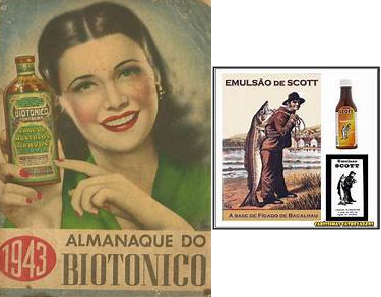
\includegraphics{C:/Users/Vermelho/OneDrive/GitHub/DonaMalvina/Imagens/BiotonicoScot.png}

\textbf{Violeta ou tintura de genciana:} para machucados.\\
\textbf{Merthiolate:} era \emph{ardido} prá caramba!, queimava mas
sarava. O Manzoni do Matarazzo falava para as crianças que era o
\emph{peida fogo}.\\
\textbf{Alho sativo (allium sativum):} para gripes e febres.\\
\textbf{Vick Vaporub:} passava nas narinas e no peitinho dos pequenos.
Faz sucesso até hoje: cura tudo!!

\includegraphics{C:/Users/Vermelho/OneDrive/GitHub/DonaMalvina/Imagens/vick.png}

\textbf{Erva de bicho e Hemo Virtus:} para hemorroidas.\\
\textbf{Lombrigueiros:} que a gente tomava e depois ficava espiando o
fundo do vaso para ver as lombrigas derrubadas.

\subsection{Simpatias caseiras}\label{simpatias-caseiras}

\textbf{Borra de panela de ferro:} para curar boqueira.\\
\textbf{Pano com rodelas de batata:} na cabeça para cefaleia.\\
\textbf{Pano entre o queixo e a cabeça:} com pó de chifre queimado ou
farinha quente para curar dor de dente.\\
\textbf{Jogar o dentinho de leite para a lua ou a estrela}\\
\textbf{Entregar a chupeta para o Papai Noel:} para abandonar o uso.\\
\textbf{Verrugas:} tinha duas simpatias infalíveis para estirpá-as: 1 -
Colocar um grão de milho na verruga e por a galinha para comer (Da irmã
do meu amigo Nelsinho Pazetti: a galinha comeu a verruga e foi só
sangue). 2 -- Passar toicinho na verruga e jogar de costas, sem olhar
para trás, dentro de um formigueiro. Minha mulher a Patrícia disse que
fez para a filha mais velha e funcionou.(A prudência recomenda não
duvidar do sobrenatural!!)\\
\textbf{Chás e mezinhas}: ruibardo, melissa, erva doce, canela, puejo,
marcela, hortelã, chá de limão ``bode'', xarope de guaco com mel.

\section{A saga do tenista Carlinhos da Dona
Malvina}\label{a-saga-do-tenista-carlinhos-da-dona-malvina}

Desanimado com as frequentes contusões no futebol, inclusive com duas
cirurgias para retirada dos meniscos enveredei para o tênis começando a
jogar no Tênis Clube de Cascavel. Em São Paulo joguei no Hobby Sports,
com várias quadras espalhadas pela capital, também no Banespa E.C e na
AABB (Associação Atlética Banco do Brasil), Swiming Center no Vergueiro,
em quadras particulares no Brooklin e Pinheiros e públicas como no
Parque Ibirapuera e no Parque Villa Lobos e mais um sem número de
quadras. Em Sorocaba na ATT -- Associação Takeda de Tênis, no Tênis Club
do Helinho perto do mercado distrital de Sorocaba. Também no Ipanema
Club, na Family e no Clube de Campo e por último no Quintela Tênis aqui
em Salto de Pirapora mesmo.

O esporte é praticado numa quadra de saibro, que exige menos da
musculatura do que em quadras rápidas e duras como as de asfalto e
Chevron (derivado do petróleo). Existem também quadras de grama onde
aumenta bastante a velocidade da bola. Joguei muito tempo em quadras
rápidas o que provavelmente desencadeou dores nas articulações e só nos
últimos dez anos, de um total de mais de trinta anos, passei a praticar
o esporte em quadras de saibro e já não aguentava mais a dureza das
outras quadras. O impacto nesses pisos mais duros repercute nas
articulações.

O Tênis é um esporte mais tranquilo para se jogar que os demais pois
evita choques e piques extenuantes. No futebol muitas vezes o jogador
fica parado lá na ponta esquerda por exemplo e participa pouco das
jogadas. Mas, quando recebe um lançamento em profundidade tem que se
esfalfar na corrida e se não estiver com os músculos bem alongados pode
sofrer sérias contusões.

O Tênis para quem não conhece é disputado em \emph{sets} . O \emph{set}
é dividido em games e termina quando um jogador fecha o sexto game,
normalmente. Há exceções mas vamos nos ater ao sexto game para
simplificar. O game é dividido em 5 pontos. A contagem é baseada nos
quartos do relógio no sentido horário (isto é teoria minha) e a marcação
é 15-30-40 e game, ou seja 4 pontos seguidos fecham o game que é contado
da seguinte maneira: 15-0, 15-15 (quinze iguais), 30-15, 40-15 e game.
Apenas o exemplo de uma variação. Os games são contados assim 1-0, 1-1,
2-1, 2-2, 3-2, 4-2, 5-2, 6-2 e fecha o set. Porquê 15-30-40 e não
15-30-45? Tanto em inglês como em português é mais fácil falar 40 do que
45. Os profissionais disputam partidas em melhor de 3 ou 5 sets, o que
faz que muitas disputas perdurem por 4 ou 5 horas, exigindo um preparo
físico e uma concentração excepcionais.

É um esporte altamente contagiante e por consequência viciante. O que se
diz que o único esporte que pode fazer um tenista mudar de opção é o
Golfe, que seria mais empolgante e viciante ainda.

O tênis é um esporte mais regular, pelo que se torna um exercício
excepcional pois movimenta braços e pernas constantemente sem grandes
alterações de ritmo, ou seja uma respiração aeróbica ritmada e contínua.
O único defeito é que se o jogador for destro movimenta mais o lado
direito do corpo em detrimento do lado esquerdo. Nesse quesito a natação
é um esporte mais completo pois movimenta braços e pernas de ambos os
lados do corpo, com perfeita sintonia, ritmo e regularidade.

Joguei tênis por cerca de quarenta anos e atribuo ao esporte o fato de
não ter me tornado obeso e ter uma boa função coronariana, além do
controle do açúcar, fugindo do diabetes. Fui um viciado total no esporte
e até um pouco fanático, não por querer ganhar apenas, mas por querer
praticar e disputar partidas o máximo de tempo possível.

Além do mais fiz excelentes amigos porquê o esporte propicia muito a
socialização. É o único esporte que conheço em que quando se mata um
ponto espetacularmente se pede desculpas ao oponente e em inglês ainda:
Sorry. Após o jogo os participantes se cumprimentam e se elogiam com
civilidade e educação e após a saída de quadra a socialização continua
no bar, estimulada por uma conversa e uma boa bebida, normalmente a
cerveja para matar a sede. O copo de cerveja mais delicioso que um
tenista toma é aquele ingerido imediatamente após uma bem disputada
partida.

\chapter{Histórias de Salto de
Pirapora}\label{histuxf3rias-de-salto-de-pirapora}

O Salto na minha época de infância/adolescência (por volta de 1.960) era
uma pacata cidadezinha do interior e assim como as demais a distração
era muito diferente de hoje. A gente se distraia indo à igreja, ao
cinema do Neto ou na folia do Carnaval ou nas quermesses. Estas além do
leilão de prendas, venda de comes e bebes sempre tinha a Banda do
Antonho Músico tocando dobrados e valsas na praça, as procissões e a
\emph{caieira} de São João. Os mais abastados da época como Agenor dos
Santos, Vicente de Nhá Cota, seu irmão Luizinho, Lauro Magno César,
Lindonor e Osteldo (que era chamado de Oster ou mesmo Ester) e outros do
mesmo calibre mandavam carros de lenha carregados de toras para a praça.
Seu Agenor já mandava num caminhão Fargo ou Studebaker.

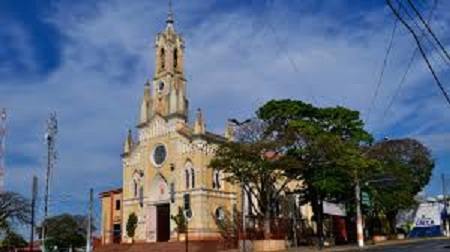
\includegraphics{Imagens/Igreja.jpeg}

\textbf{Matriz de São João Batista, no mesmo lugar onde foi inaugurada
uma capela em 1907}

Esta lenha era empilhada em forma de \emph{caieira} ou seja trançando as
toras e se erguendo por 4 ou 5 metros. Na \emph{véspa} do dia de São
João Batista, padroeiro da cidade era acesa a caieira e isso tinha um
cerimonial todo especial. Vinham o festeiro, o prefeito, o padre, o
delegado (que não era de carreira mas um cidadão comum) e o povo que
tinha saído da igreja após a missa, mais a molecada e os que vinham prá
\emph{sapiá}. Acendiam o fogo e aí começava o \emph{samba} que de samba
não tinha nada. Era um improviso de versos mais ou menos em ritmo de
cururu. Ia chegando a turma do Lúcio Camargo, com seus bumbos artesanais
feitos de couro curtido de boi. Os cantadores dos quais me lembro
vagamente da turma do Lúcio Camargo eram o Joaquim Furquim e o Pinhé. O
Timóteo também andava por ali,pois era onipresente em todas ocasiões
sempre ralhando e correndo atrás dos moleques arteiros como eu que
jogavam pedregulho na tuba da banda. A cachaça rolava solta, tomada
\emph{no gargalo mêmo} e o samba \emph{comia o couro}, madrugada
adentro. Eram versinhos já consagrados ou improvisos. Só me lembro de um
deles cantado pelo Lúcio Camargo. Era assim: Sabiá na laranjeira, avoô e
sentô, avoô e sentô, avoô e sentô e o surdo marcava firme o ritmo e esta
cantilena se repetia infinitamente porque não havia mais versos nesse
improviso. Era muito simples mas muito bonito pela pureza e inocência
dos improvisadores e das músicas. O litro de cachaça ia passando de mão
em mão, e o clima ia esquentando. Varavam a noite cantando e sambando
até acabar a cachaça e a fogueira, no sentido ambíguo da palavra. A
pinga não raro era renovada por alguma alma boa que gostava da farra e
não queria que parasse.

\section{O Leilão de Garrotes}\label{o-leiluxe3o-de-garrotes}

Era outra distração. Os fazendeiros mandavam garrotes ou novilhas como
prendas, para renda da igreja ou do asilo, e esse gado era leiloado na
mangueira do Seu Genor, na Granja em frente ao atual Asilo dos
Velhinhos. Os arrematantes se empoleiravam nas tábuas da mangueira para
avaliar as \emph{criação}, e o leiloeiro ficava dentro da mangueira à
uma distância razoável dos garrotes e ia repetindo os lances. Para
esquentar e dar coragem alguém abria uma garrafa de conhaque São João da
Barra e ia tentando entusiasmar os \emph{dinherudos} que podiam
arrematar algumas cabeças ou mesmo um \emph{lotinho}. Um dos
arrematantes sempre presente era o Vicente da Nhá Cota, um dos mais
\emph{carçudo} em matéria de dinheiro e o festeiro mandava o
\emph{samiadô} de bebida \emph{tacá} conhaque no Vicente. Numa certa
altura ele percebendo que queriam \emph{deixá ele bêbido pá morde de
abrí a argibêra se virô p´o o bebideiro e falô: Óia, a partir de agora
nóis semo sócio. O que eu arrematá você tem que pagá a metade}. O
bebideiro caiu fora rapidinho percebendo a esperteza do Vicente da Nhá
Cota.

\section{O Boi de Cesto}\label{o-boi-de-cesto}

Nos carnavais de Salto de Pirapora uma figura muito conhecida na época,
o Pinhé, fazia um boi de cesto junto c´o Chico Branco, que cuidava e
morava na Caixa d´água, atual Sabesp. O corpo do boi era feito de
taquara trançada e colocados uma cabeça e um rabo de boi. Num espaço no
meio da armação o Pinhé entrava e saía carregando o boi de cesto. O
cortejo de curiosos que sabiam da brincadeira acompanhavam o boi até a
praça em frente à Matriz e o boi saía correndo atrás de um passante
qualquer ameaçando chifrar e berrando: Móóóóó. Cheguei a ver o boi
entrar dentro do bar do Tonico da Mulatinha atrás de um gaiato que fazia
\emph{fusquinha} provocando o boi. Isso lá pelos idos dos anos 60. Na
minha época já na década de 80 revivi a brincadeira do boi de cesto e o
\emph{boi} era o Paulinho Mixirica, forte o bastante para carregar a
armação, louco por uma farra, com a cara pintada. O Paulinho adorava se
vestir de mulher no carnaval. Então pintar a cara para êle era um
verdadeiro deleite. Só que chegava uma hora, de tanto correr e tomando
umas para animar não aguentava mais e passou o boi para o Balaio que
também já estava bem \emph{artete}. A molecada para provocar puxava o
rabo do boi e o Balaio mole de cachaça: Num puxe o meu rabo, móóóóó.

\section{As quermesses da Festa de São
João}\label{as-quermesses-da-festa-de-suxe3o-jouxe3o}

Minha mãe Dona Malvina contava que na época de tais festas ela preparava
quitandas para vender na festa. As quitandas eram biscoitos de polvilho,
rosquinhas doces, bolo de amendoim, cocada em calda e outras delícias.
Tinha o leilão de prendas em frente à igreja. As prendas poderiam ser
desde uma réstia de cebola, um frango assado, um delicioso cuscuz de
sardinha (me deu água na boca só de lembrar), um frango vivo ou assado,
um leitão, um bolo de milho verde e por aí afora. Tinha a banda tocando
\emph{uns dobrado e umas vársa}. Mandavam fazer uma \emph{cadeia} de
bambu para prender as pessoas. Escolhia umas moças bonitas que pegavam
os homens pelo braço e levavam \emph{preso}. Fechava a porta da cadeia e
só saía se pagasse a fiança. Eu consegui numa das festas reviver e
recriar essas lembranças, que só conheci pelo relato da Mamãe.
Infelizmente não pudemos levar a festa até o final por causa das minhas
brigas com o Padre Francisco. Eu queria terminar a festa, fazer um
balancete apurando o lucro, separar uma parte para fazer um baile e
repassar o restante para a Igreja mas, antes disso o padre exigiu o
repasse total e imediato da arrecadação.

\section{Baile de sanfona na casa do Chico
Branco}\label{baile-de-sanfona-na-casa-do-chico-branco}

O Chico Branco, aquele do boi de cesto, tio do Merquides, do Dito Fisga
e da Cacirdona era o responsável por tomar conta da Caixa dágua, atual
Sabesp e gostava de fazer bailes na sala da sua casa. Chamava um
sanfoneiro, tirava \emph{os trem} da sala para \emph{abrí espaço} e a
coisa esquentava. Eu, na flor dos meus dezoito anos mais ou menos, tava
paquerando a filha da Cacirdona, irmã do Fião. Prá facilitar as coisas
tirei a Cacirdona prá dançar e ela, dona de portentosa bunda, dançava
muito bem. Eu rodopiei a sala com ela mas não resisti quando vi uma fila
de garotos enfileirados na parede, uns cinco ou seis só assistindo. Dei
uma embalada no ritmo da música e no começo da fila, dei uma virada
brusca, e a bunda da Cacilda fez um \emph{strike} na molecada.
\emph{Disgrudô} todo mundo da parede. Alguém se vingou de mim e foi no
meu fusca vermelho encostado lá fora e fizeram um ``U'' nas placas
entortando o quanto deu as abas das chapas. Outros bailes famosos na
época foram os do \emph{Macuco} e parece que o Áureo da Bertília (eram
um casal na época) também fazia bailes mas nesses eu nunca fui.

\section{O Clubinho no centro}\label{o-clubinho-no-centro}

Mais ou menos onde está hoje a loja de móveis Gianini, bem em frente à
casa do Zé Martelo, era o nosso clubinho, um salão alugado do seu Agenor
dos Santos. Criamos uma pequena associação, a SASP, Sociedade Amigos de
Salto de Pirapora e começamos a fazer bailes que marcaram época na
região. Nossa turma: Nazírio Caetano, a família toda do Romãozinho, o
Eli do Girso, a garotada do seu Olézio, Naile e Sid do João Friage,
Sidney Estofadinho (eu apelidei) do Aristide Farrapo, Zé Carlinho do
Moacir Padêro, Galo, Mirinho e Cláudio da Ditinha do Mirão, Paulinho e
Nenê do Paulo Padeiro, a Jurema e a Lúcia do Seu Antonio Padeiro e da
dona Aparecida, o Lino Castellani, Miguel do Paco, Miguel e Seme Hadadd,
Levi Seabra, filho do Seu Gênio do Armazém da fonte, Maria Helena e
Miguel Mandu, a Ditona e a Preta, irmã do Zé Cadela pai, que moravam no
Matarazzo, a Sida e a Nice do João Leandro, a Tereza japonesa, a Mérça
do Calico, a Sirley do Dito Coelho, irmã do Zé Carlão, a Noemia do
Neguito, neta de dona Virgulina e outros tantos. Um grande entusiasta e
com boas idéias para os bailes era o Nilson do Feliciano e da Dona
Ordália, que eram donos do atual bar do Cochinha. Depois o Tonico da
Mulatinha, irmão do Feliciano comprou esse bar que também foi do
Romãozinho, tocado pelo Renê e pelo Tide.. A Marlene fazia inesquecíveis
pasteizinhos de carne que quando a gente mordia escorria um caldinho de
tomate pelo canto da boca. Irresistíveis. Isto em meados dos anos
70/80.\\
Na época contratamos os conjuntos Kingstones e Flipers de Sorocaba. No
primeiro o guitarrista era o Zé Carlos Benedetti, eterno engenheiro da
Prefeitura. Os bailes ficaram famosos em toda a região e os carros
estacionados chegavam a tomar a rua inteira do centro. Uma proeza e
tanto para a época, pois pouca gente tinha carro próprio. De Pilar
vinham o Zé Maria e o Tucha do Genésio da farmácia, o Véia, o Neto, o
Ademar Proença, o Nézinho que tomava conhaque e comia chocolate junto.
De Sorocaba vinha o Edson \emph{Pinta}. De Sarapuí vinha a Neusa Holtz,
com um bando de sobrinhas bonitas, entre elas a Vera Holtz, atriz global
que curtiu muito os nossos bailes. Pelo menos uma vez trouxemos também
para tocar o Supersom TA e o Biriba Boys do Ciço Benedetti (irmão do
Walter Benedetti) muito famoso de São José dos Campos que depois mudou o
nome para Tropical Quintet.

\section{O bando de anus}\label{o-bando-de-anus}

Para quem não conhece os anus (estamos falando nos passarinhos não no
que você está pensando!) são pássaros pretos (pelo menos aqui na nossa
região eles são pretos, mas existem anus brancos, como o da direita na
foto) que vivem em volta dos taquarais ou nas tigueras (soqueiras na
região de Cândido Mota) de milho.

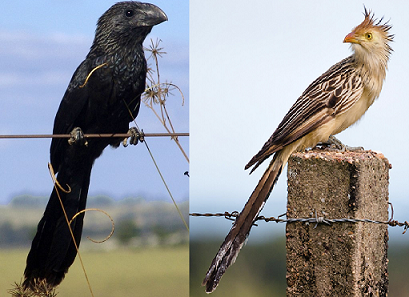
\includegraphics{C:/Users/Vermelho/OneDrive/GitHub/DonaMalvina/Imagens/anu.png}

Adoram fazer ninhos e algazarra nos taquarais. A nossa turma de Salto de
Pirapora, que normalmente alugava a Kombi do Aristide Farrapo, ou do
Elia Gêlo para ir aos bailes da região auto apelidou-se de \emph{bando
de anu} porquê normalmente vestíamos ternos pretos e andávamos em bando,
fazendo algazarra.

\section{O baile da lama em Piedade}\label{o-baile-da-lama-em-piedade}

Fomos num baile em Piedade, no clube da Praça, o PFC (Piedade Futebo
Club) , e na volta com uma chuva torrencial, vindo pela estrada de terra
do bairro dos Leites a Kombi encalhou no meio do barreiro numa daquelas
subidonas, lisas que nem um sabão. A Kombi empacou, o motorista
acelerava e ela \emph{saía de banda}, ameaçando ir prô barranco. O
motorista pediu prá todo mundo descer e empurrar. Foi um tal de arrancar
as fantasias de anú, formar aquele bando de homens de cuecas, camisas
brancas de mangas compridas e alguns de gravata ainda. Pena que não
havia celular para registrar a cena. Virou um bando de nús. Hoje seriam
nudes.

\section{O baile do pijama do Seme em
Araçoiaba}\label{o-baile-do-pijama-do-seme-em-arauxe7oiaba}

Outra viagem de Kombi para Araçoiaba. No início os bailes eram num
clubinho bem no centro, na praça da Igreja matriz. Um salão com janelões
baixos por onde a gente pulava quando saía briga no salão e alguns caras
de pau pulavam mesmo para entrar sem pagar. O Seme Hadadd, filho do Zé
Turco e da Jovita, tinha comprado um pijama novo, daqueles antigos,
listrados de mangas e pernas compridas, típicos dos que só se usavam
quando se internava num hospital. Lá pelas três da madrugada, o baile
roncando o Seme vai para a Kombi, veste o seu pijama, estalando de novo,
e bota o cabeção na janela no intervalo da seleção musical gritando:
\emph{Ei turma, vam´bora que eu tô cum sono: quero dormí}. Na verdade
ele queria era exibir o pijama novo. Tempos depois o clube mudou para o
local do antigo cinema, na mesma praça, uns cem metros abaixo na direção
do lago. Acontece que o cinema, para permitir uma visão melhor da tela,
era em desnível, ou como se dizia: o salão tinha discaída*. Dançando
ladeira abaixo era uma maravilha mas ladeira acima era uma dureza.

\section{Os bailes da região}\label{os-bailes-da-regiuxe3o}

Nós, os jovens \emph{baileiros} de Salto de Pirapora sempre gostávamos
de ir aos bailes de Pilar do Sul, apesar da eterna rivalidade das duas
cidades vizinhas. Mas, conosco era diferente: nunca arrumamos brigas,
éramos bem recebidos e os recebíamos bem em Salto, nos nossos bailes.
Fizemos lá grandes amigos como Zé Maria e Tucha, João Marcolino, o
Nézinho (viria a ser cunhado do Júnior da Shirle) que infelizmente
morreu novo de tanto beber, o Véia dentista, que morreu velho mas
bebendo bastante, e tantos outros. Havia um costume em Pilar do Sul de
interromper o baile no meio e fazer um leilão para arrecadar fundos. Num
desses bailes estávamos eu, Miguel do Paco (Miguérzinho Espanhór),
Miguel e Seme Hadadd, Zé do Lico, Lino Castellani, Galo (Celso irmão do
Zé Quito), Mirinho e outros tantos levados provavelmente na Kombi do
Elía Gêlo, ou do Aristide Farrapo ou do Arcide ou ainda a do Nezinho
barbeiro. No meio do baile começou o leilão e a certa altura foi
leiloado um cuscuz . Prá quem não conhece é feito num cuscuzeiro com
massa de farinha de milho com sardinha e ovos cozidos. Quando
desenformado e colocado num prato de \emph{ponta cabeça} ficavam
aparecendo os ovos cozidos cortados em rodelas destacando o branco e
amarelo por fora e as sardinhas enfileiradas inteiras. O leilão estava
fraco de interessados e o leiloeiro, muito esperto, resolveu provocar:
\emph{20 cruzêro no cuscuiz e a turma do Sarto num cóme cuscuiz}. O
Miguel Espanhol já se sentiu provocado: \emph{30 conto e a turma do
Sarto vai cumê cuscuiz sim. O pilarense: 40 miréis e ôceis num come. O
Miguér: 100 conto e nóis cóme}. Não teve jeito e veio o cuscuz prá nossa
mesa feito um troféu. Todo mundo já bem \emph{artete} (bebuns) e naquela
altura do campeonato ninguém tinha vontade de comer cuscuz. Um foi lá,
tirou um pedaço de ovo, outro uma lasca de sardinha e por aí foi até o
cuscuz virar uma verdadeira cratera lunar esburacada. O Miguel Ortiz,
muito \emph{beudo} olhou para o cuscuz: Essa bosta me custou cem conto.
Botou a mão por baixo do prato e jogou prá cima. Não é que prato e
cuscuz deram uma pirueta no ar e voltaram na mesa na mesma posição
original??????? Coisa de bêbado mesmo. Num outro baile em Pilar do Sul
mesmo, fizeram um leilão de um bezerro, que foi trazido pro salão
arrastado pelas orelhas. Assim que adentrou o salão o bezerrinho,
assustado e medroso, deu uma \emph{cursada} daquelas do tipo \emph{riscá
campo de futebor com cár. Espalhou merda pô salão intêro}. Foi uma
correria de gente procurando sacos de estopa para limpar a sujeira. E o
baile continuou. Com cheiro de mangueira. Também frequentamos muitos
outros bailes na região: Recreativo e Sorocaba Clube, ainda no
tradicional clube da Praça Coronel Fernando Prestes no centro. Houve uma
época que o Recreativo foi comandado pelo Pedrinho Salomão que fez
grandes bailes e com decoração do Alcides Guimarães. Grandes conjuntos
de baile se apresentaram por ali: Super Som TA, Orquestra de Tupã,
Biriba Boys e Modern Tropical Quintet e o Casino de Sevilla, que na
época estava no seu melhor esplendor.

\section{A sacaria do Aristides}\label{a-sacaria-do-aristides}

O \emph{Aristide}, da grande família dos Mandu: João Mandu, violeiro e
compositor, Antonho Mandu, violeiro e mariano da Igreja Católica,
Zequinha Mandu etc etc montou uma sacaria, uma pequena empresa
praticamente de fundo de quintal, que funcionava nos fundos do Armazém
do Zé do Santo. O Aristides comprava sacaria de papel usada, mandava
desmanchar os sacos, virava-os do avesso e carimbava com o novo nome, Ou
seja, faziam uma reciclagem. Ali trabalhavam o Orlandinho do Iúta, o
Waldemar, o Flavinho, o Lagartinho e outros. Todos craques de bola. O
Waldemar chegou a se profissionalizar no São Bento de Sorocaba mas não
deslanchou apesar de ser um cracaço de bola. O Aristides era corinthiano
roxo, fanático mesmo e essa molecada toda mostrava simpatia ao
Corinthians por questão de sobrevivência na firma. Um dia o Aristides
prometeu aos moleques, todos simples e de origem humilde que os levaria
para ver um jogo do Corinthians no \emph{Paicaimbu} em São Paulo.
Promessa feita, promessa cumprida. Lotou sua Kombi sacarieira e partiu
para São Paulo, via Raposo Tavares pois ainda nem existia a Castelo
Branco. No alto da Serra entre São Roque e Cotia havia o Restaurante do
Alto da Serra. Ali serviam um comercial famoso pela fartura. Nada de PF
o malfadado prato feito. O Aristides desembarcou os meninos, que foram
com muita vergonha e com o melhor de suas roupas simples para a mesa de
jantar. O Aristides na cabeceira comandando o festim. Primeiro foi
servida a sopa naquelas terrinas fundas, fumegando de quente,
acompanhada de pão à vontade. O Flavinho, pediu para encher o prato
fundo por umas 3 vezes. Estava acostumado (como todos nós) ao fato de
que quando havia sopa em casa era sopa e mais nada. \emph{Bateu} as três
pratadas acompanhadas de vários \emph{filãozinho}. Novidade também para
os garotos acostumados ao pão sovado ou o filão grande, cortado pela mãe
na barriga com a faca de serra. Acabou de tomar a sua sopa, cruzou os
braços e ficou ali comportadinho esperando e achando que a janta já
tinha acabado. Começaram a servir o jantar propriamente dito: pequenas
tigelas de feijão, arroz, batatas fritas, fígado de boi, batata doce,
carne ensopada, macarrão com carne moída e outros que tais. O pessoal
comendo e o Flavinho quietinho de braços cruzados. O chefe ordenou: Coma
Flavinho, tire arroz, tire feijão, carne, batatas. E o Flavinho:
\emph{Deus que azúde seu Alistide, tô sastifeito}.

\section{O Time dos Paradinho}\label{o-time-dos-paradinho}

Com a fama do time dos Parados, a ser contada adiante, surgiu o time
juvenil com o nome de Paradinhos. O treinador era seu Dito Coelho, pai
da Cirley e do Zé Carlão. Ali brilhavam os mesmos craques da Sacaria do
Aristides: Waldemar, Orlandinho (tio do Waldemar), Lagarto, Flavinho,
Rodeirinho, Jaime Vigorelli (tinha esse apelido porquê parecia uma
máquina de costura nos dribles). Entrei para os treinos no time e logo
fui adotado pelo Flavinho, que adorava \emph{amaciar uma bola no peito}
no meio de campo, arredondava e gritava: Corre Carlinho: lançamento
perfeito, por cobertura por cima dos beques e eu disparando lá no corner
direito: era ponta direita. Aí dominava e tinha que enfrentar os
beques-cavalos Dorfão e Zitão. Num desses treinos eu cheguei antes e
fiquei brincando ali pelo campo, \emph{petecando bola e escabeceando no
gol}. Minha mãe fez prá mim um bibi. Era um boné tipo militar com um
bico na frente e outro atrás. O Nambu (o pai, Mizael) que adorava judiar
dos mais novos arrancou meu bibi da cabeça com um tapa e encheu de
areia. Segurei prá não chorar. Iria pegar mal. Começou o treino. No time
adversário Nambu no gol, Gastão (Dorfão) e Zitão a dupla de beques
trogloditas. O Zitão não era cavalo que nem o Dorfão mas duro de passar
por ele por ser alto. E o Nambu me provocando do gol: bostinha, boné de
viado, \emph{fiinho da mamãe}. Lá pela metade do primeiro tempo,
Flavinho mata a bola no peito, amortece e lança. Eu sozinho na ponta
direita, vim fechando para o gol. Primeiro veio o Zitão, dei um corte
prá direita e deixei comendo poeira. Na sequência vem o Dorfão com
aquele pé de foice, roçando vento perna e o que mais viesse pela frente.
Na mesma sequência do primeiro corte, dei o segundo prá esquerda e saí,
frente a frente com o Nambu. Eu com aquela sede de vingança. O Nambu
veio e se jogou na minha frente para abafar a jogada e tentando me
derrubar com bola e tudo. Na maldade mesmo. Dei um toque na bola por
baixo do barrigão e a bola foi caminhando lentamente para o fundo das
redes. E eu caindo por cima do Nambu. Quando me dei conta de que estava
por cima dele, o cotovelo a 5 cm daquela cabeça de bola de capotão não
resisti, ergui o cotovelo mais alguns centímetros e desci com tudo.
Senti a cabeça dele \emph{pururucar} contra o chão seco do campo do
Bumbo, atrás da antiga Prefeitura. Foi o tempo de bater, levantar
e\ldots{}\ldots{}\ldots{}\ldots{} correr. Prá não apanhar. O bicho
bufava. Mas nunca senti um gosto de vingança tão saboroso. Tive que
correr dele naquele dia e em muitos outros mais, pois o danado virou
juiz de menores e ia no clubinho onde eu comandava os bailes e eu tinha
que aturar a \emph{metideza} dele. Exigia entrada e cerveja de graça
para ele e ainda tinha o topete de levar puxa sacos agregados para beber
de graça. Ainda xingava a molecada que me ajudava no bar do clubinho.
Depois passou, viramos amigos e tudo foi esquecido. Hoje sei que luta
muito com a saúde e desejo que leve a melhor. Aquilo tudo ficou no
passado mas fez parte do folclore da minha vida.

\section{As festas de Primeiro de Maio do Seu
Olézio}\label{as-festas-de-primeiro-de-maio-do-seu-oluxe9zio}

Olézio dos Santos trabalhava na Coletoria de Impostos, órgão estadual.
Casado com a Dona Zuza, pessoa muito simpática e hospitaleira. O casal
gostava de receber pessoas em sua casa mesmo antes de construir a grande
residência da Rua Vicente Ferreira dos Santos, onde é hoje o Ciretran.
Tinham uma penca de filhos: o Paulo, o Tomáz, o Antonio Marcos e o Pedro
Geraldo, e as meninas Ana, Tarsila e Sílvia. Naquela época que poucas
casas tinham TV era uma festa assistir um jogo na casa do \emph{Seu
Lézio}. Dona Zuza estourava grandes baciadas de pipoca, por repetidas
vezes e aquilo se tornava um programa muito legal: assistir os jogos na
TV, comendo pipoca e sentado num sofá, coisa rara nas nossas casas.
Outra característica da casa era uma mesa redonda com uma roda menor no
centro, que girava sobre o próprio eixo, levando os pratos para a outra
ponta da mesa com um mínimo de esforço. O Olézio sempre foi polêmico,
mas estava sempre brigando do lado dos fracos. Uma vez fez um discurso
veemente nas arquibancadas do campo dos Parados. Num chute mais forte a
bola do jogo foi parar no quintal do João da Nhá Cota e este não queria
devolver devido à velha rincha futebolística e política: Bumbo versus
Parados, turma do João Guimarães contra a turma do Genor do Santo.
Depois do discurso contra a arrogância bumbense a bola foi devolvida
depois de vaias e no final aplausos. Só tinha aquela bola para continuar
o jogo.\\
Muito bem: Seu Olézio organizou uma festa de Primeiro de Maio inédita na
cidade e que se tornou depois uma tradição e marcou época entre os
poucos eventos da cidade. Convidou várias empresas para que montassem
suas equipes para disputar diversas provas: campeonatos de cabo de
guerra, de truco, de futebol, gincanas e no final um desfile começando
no largo da Fonte e passando pela praça da Matriz, onde se instalou um
palanque para as autoridades, os organizadores e as Rainhas de cada
equipe. Assim, o Matarazzo, a Incalesa, a Cosipa, o comércio, o setor
rural montaram suas equipes para disputar as diversas provas e
somando-se os pontos chegava-se ao campeão. Tinha também a princesa de
cada equipe que ao vencer o certame também somava pontos. Vencia quem
vendia mais votos. Eu participei pela Matarazzo e venci uma gincana que
tinha baliza de estacionamento, acertar uma bola no gol e outras
dificuldades. Minha parceira foi a Maria Helena do João Mandú.\\
No cabo de guerra o Matarazzo tinha o Lazão, o Gustão de Moraes, o
Curingão e o Gentirlão da PonteArta, o peso pesado de cerca de 140
quilos que ficava na ponta da corda. O Curingão até hoje mostra com
orgulho a medalha que ganhou junto com a sua equipe. Quem também
participou, pelo comércio foi o Joel Haddad e o Jobão, um touro de
forte, fiel funcionário da turcada por muitas décadas. As que disputaram
como Rainhas foram a Elizeth do Genorzinho, a Nice do Correio, a Cirley
do Matarazzo, a Noêmia do Neguito, a Celinha e a Regina Mascarenhas,
lindíssimas e que vinham de Sorocaba especialmente para competir pelo
setor Rural. O Genorzinho, pedreiro e construtor de cortiços se gabava
de \emph{ter gastado 5 mil na reforma da fia} prá participar do
concurso.

\section{\texorpdfstring{A turma do
\emph{Matarazzio}}{A turma do Matarazzio}}\label{a-turma-do-matarazzio}

O caminhão \emph{pau de arara} que levava os trabalhadores de Salto para
a fábrica Cimimar, mais conhecida como Matarazzo, ou \emph{Matarazzio}
pro Gustão, pai da Zilda e da Maura que falava de boca cheia: \emph{Eu
trabaio no Matarazzio}. Esse caminhão era chamado de pau de arara,
talvez numa referência aos paus de arara que traziam nordestinos para
São Paulo em busca de trabalho. Era um caminhão de carroceria toda
fechada de zinco, inclusive no teto, com uma cortina de encerado na
frente para amenizar a poeira na seca e o vento frio no inverno. Atrás
tinha uma escada de ferro para facilitar o acesso e na carroceria dois
bancos laterais. Eu trabalhava no escritório em horário diferenciado dos
operários da fábrica, do forno e outros setores. A turma que fazia parte
no horário das 7.30 hs: Jorge Faustino, Antonio Brandini, Toninho
Amâncio, Lazinho da Lina da Mulatinha, Laerte, Ditinho Brandini, Ditão
do Arcidão, Zé Bode e eu também. Seu Jorge Faustino era um mitômano
compulsivo, ou seja viciado numa mentira. Mas as suas mentiras eram
floreadas, cheias de charme e o fazia com uma seriedade tão grande que a
gente tinha receio de duvidar ou dar risada. Incluía datas e endereços.
Por exemplo: \emph{Sabe? (usava muito essa expressão) No ano de 1958 no
Rio de Janeiro na Rua Alice número 254 existia um rendez-vous (o popular
puteiro) muito chique com lindas mulheres de alta classe onde eu sempre
frequentava\ldots{}\ldots{}\ldots{}..} E ia por aí fora citando nomes e
detalhes criados na sua fértil imaginação. Contou uma vez, com grande
seriedade e circunspecção que foi pescar num rio muito largo e preparou
como isca um belo pedaço de carne. Pescaria de linhada. Virou a linhada
em volta do corpo por várias vezes e arremessou com tanta força, mas
tanta força que não viu a isca cair dentro do rio. Ficou na espera: de
repente começou a puxar forte e pesado. Linhada comprida: mais de 50
metros. Foi puxando, puxando, cada vez mais pesado até que trouxe a
presa até a beirada do rio. Qual a surpresa quando viu que tinha fisgado
um\ldots{}\ldots{}\ldots{}. cachorro do mato. A força do lançamento foi
tão grande que a linhada atravessou o rio caindo bem em frente ao tal
cachorro do mato. \emph{Durma c´uma buia dessas}. E desse risada ou
tirasse sarro. Ele repetia toda a história com provas e argumentos mais
contundentes ainda. Melhor ficar quieto e engolir em seco. Robatão,
encarregado da Mecânica. Sério e circunspecto raramente deixava escapar
um sorriso contido, disfarçadinho de lado, ouvindo as \emph{proezas} do
Seu Jorge. Luiz Pereira, o Luizinho, era o chefe do escritório e viajava
na cabine do pau de arara, junto com a Cirley, funcionária do Posto de
Abastecimento. Viajar na cabine era lugar de status na hierarquia
Matarazziana. Eu pude viajar ali quando substituí o Luiz Pereira que
após quase vinte anos de empresa, foi obrigado pelo Escritório Central
em São Paulo (hoje Prefeitura Municipal, no viaduto Anhangabaú) a entrar
em férias e eu, o mais novo de idade e de empresa fui encarregado pelo
Diretor Engenheiro Wilmos Istvan Toth (o chefão geral) a \emph{tirar
férias} do Luizinho, que vinha se recusando a \emph{sair} de férias para
não largar o osso do comando do escritório. Tinha mais ciúme do cargo do
que da mulher.\\
O Chiquito Rosa (pai do Mamute e do Chiquitão), o Querubim (nome de
anjo, filho do Zé Fredão e irmão da Joilda e do Joelmir) e a Cirley eram
funcionários do Posto de Abastecimento, uma espécie de armazém que
revendia produtos da própria Matarazzo: sabão em pó, óleo de cozinha,
açúcar Amália produzido na fazenda do mesmo nome, bolachas, macarrão etc
da marca Petybon e uma infinidade de produtos da própria empresa. Esses
produtos só eram vendidos aos funcionários para desconto em folha de
pagamento, e isso gerava uma verdadeira caçada dos mesmos por pessoas de
Salto que queriam os produtos de qualidade da empresa, não encontrados
no comércio local (vendas do Zé do Santo, Zé Turco, Eugenio Seabra).
Naquela época não havia supermercados na cidade.\\
Ditinho Brandini, que trabalhava com Custos, franzininho e que num jogo
de futebol no campo dos Parados em que atuava como juiz de futebol levou
um tapa na orelha do Balaio. Com medo de apanhar mais, o Ditinho se
jogou no chão com a mão na orelha, chorando que nem criança. Cena
hilária que eu assisti ao vivo da arquibancada.\\
Lazinho, casado com a Lina da Dona Mulatinha, e o Agenor Teixeira (pai
do Joninha) eram os encarregados de tirar Notas Fiscais. Estas notas
eram datilografadas e passadas para um rolo de gelatina e depois
copiadas num livro enorme de difícil manuseio (no chute: de 80 x 40
cm.). Usava-se no processo um carbono roxo, chamado copiativo,
específico para copiadoras de gelatina, que deixava as mãos todas
pintadas de quem as manuseava. Se levava a mão no rosto, a cara ficava
toda roxa.\\
Laerte, responsável pela folha de pagamentos, único filho da Dona Zica e
de pai incógnito, criado pela mesma \emph{com todo o leite} como dizia o
meu pai, comparando filhos mimados com bezerros de vacas das quais não
se tirava o leite e ficava tudo para a cria. Ou seja o Laerte tinha
todas as regalias que a gente invejava. Ganhou da mãe uma bela casa no
centro e uma das poucas com televisão aonde íamos em bando assistir
jogos de futebol e tomar cerveja. O Laerte era meu chefe, bebia muito e
tinha uns repentes de mau humor quando ficava dias sem falar com
ninguém. Um dia, não sei porquê cargas d´água me passou uma rasteira
dentro do pau de arara, todo sujo de lama. Caí de costas e tive que
trabalhar com barro da cabeça ao calcanhar. Não tinha como me trocar.
Numa das vezes que fomos ver jogo televisionado (um luxo) na casa dele
tava o Zé do Lico. Era quem levava correspondência para o escritório
central na capital. O Zé tinha tomado várias e dormiu no sofá durante o
jogo. Nisso entra uma propaganda da caninha \emph{Yaúca}, quem se
lembra?. O Zé do Lico acordou assustado: Quem que é esse tar de Iaiúca
que entrô no time do Parmêra???? Outros que não viajavam no nosso pau de
arara e que merecem ser lembrados Dorfo Bode, encarregado da pedreira
Dolomita. Pai do Dorfinho, Rosalvo etc. etc. etc. Rodolfo foi vereador
nos tempos do Izidorinho, Bertinho Marcelo e outros (época pré Dito
Pão). Eu era secretário da Câmara e redigia as atas: quietinho num
canto, só fazendo anotações e sem direito a dar um pio e muito menos uma
risadinha. Nisso começa uma discussão entre o Dorfo Bode e o Izidorinho.
Este um homem de baixa estatura mas bem brabinho e fanático por
politicagem. Como diria meu pai Pedro Orive: por ser pequeno a brabeza
num tinha prá onde ir e ficava concentrada. Já tinha havido discussão
numa sessão anterior e ocorreu a seguinte pérola de diálogo. Rodolfo: Na
úrtima sessão Vossa Incelência me chamô de burro!!!!!! Izidorinho: Eu
num chamei Vossa Incelência de burro não!!!!!! Rodolfo: Vossa incelência
chamô \emph{minha} Incelência de burro sim!!!!! Só \emph{se rindo}, mas
o secretário tinha que ficar de boquinha fechada. Figura constante no
pau de arara era o Calixtro, marido da Dona Leonor, pai do Dirceu Sebo,
do Dineu Lindóia e da Dircéia do Robatão. O Calixtro era um \emph{hóme
brabo}, sempre de cara feia, vestido no estilo boiadeiro e com um
indefectível \emph{paiêro} fedidíssimo no canto da boca. Além de tudo
estava sempre acompanhado de um cachorro fedorento e mau humorado que
gostava de cheirar todo mundo. O Calixtro, como pai do Dirceu Sebo, que
era chefe da Vigilância, puxa saco de plantão do Baroni (gerente
administrativo) tinha direito a se utilizar do pau de arara quando bem
entendesse mesmo sem ser funcionário e ainda por cima abusava dessa
posição hierárquica, digamos assim de natureza \emph{puxa-saquista}, por
parte do filho Dirceu . Um belo dia o cãozarrão foi cheirar o André, que
depois trabalhou na Prefeitura, e este ameaçou chutar o cachorro. O
Calixtro enfezou: Porquê tá chutando o meu cachorro. E o André, bem
enfezadinho também, devolveu na lata: \emph{Se cherá eu de novo eu chuto
o cachorro e chuto o dono tamém}. Foi a primeira pessoa que vi desafiar
o Calixtro. E era um garoto, \emph{de menor} ainda. Na minha vida formei
vários garotos, ensinando tudo que sabia inclusive o \emph{pulo do
gato}. Na Matarazzo, pedi um auxiliar para o departamento pessoal que
comandava sozinho, substituindo o João Machado e o Dineu. Escolhi o Zé
Carlinhos, menor de idade que entrou como aprendiz na oficina mecância
mas, que naquele momento fazia valetas no campo de futebol, talvez pela
falta de paciência dos mais velhos em lhe ensinar mecânica. Ele veio de
macacão, sujo de terra, conversar comigo na janelinha do departamento
pessoal e pediu para voltar depois do almoço, de banho tomado e de
roupas condignas para entrar no escritório. Como ele tinha feito curso
de Datilografia, dei-lhe um método e fiz relembrar a prática da máquina
de escrever por uma semana seguida. O dia inteiro batucando na máquina
mas quando terminou o treino estava um craque, quase tão bom quanto o
mestre que aliás digita até hoje sem olhar para o teclado. Fui então
passando todo o serviço para ele que, com muita vontade de trabalhar no
escritório e ele e a família orgulhosos pela nova função, aprendeu
rápido e quando resolvi deixar a empresa ele ficou no meu lugar e mesmo
depois de aposentado continuou trabalhando para as firmas que sucederam
a Matarazzo, que infelizmente \emph{virou pó} pela má gestão da famosa
terceira geração fazendo juz ao ditado: \emph{Pai rico, filho nobre e
neto pobre}. Um verdadeiro império de empresas iniciado pelo fundador
Francisco Matarazzo que diziam ter começado vendendo banha de porco de
porta em porta em Sorocaba. No auge tinham mais de 300 empresas no ramo
de mineração, têxtil, celulose, produtos de limpeza, produtos
alimentícios e por aí afora. Na geração de Maria Pia Matarazzo tudo foi
por água abaixo, literalmente.

\section{A política em Salto de Pirapora nessas épocas (sou péssimo em
datas)}\label{a-poluxedtica-em-salto-de-pirapora-nessas-uxe9pocas-sou-puxe9ssimo-em-datas}

Como sempre se soube a política em Salto de Pirapora sempre foi dominada
pelo Agenor Leme dos Santos, o seu Genor. Um eventual adversário foi o
João Guimarães, pai do \emph{Nirto Guimarães} que depois viria a ser um
folclórico prefeito, trinta anos depois. Outros de oposição eram a turma
dos Marcellos: Bertinho, Zé Carroça, João da Nhá Cota dando suporte mas
nunca ameaçaram o reinado do Seu Genor, que era dono de pedreiras, da
Incalesa, de grandes sítios, da Granja em frente ao asilo, o qual foi
ele que fundou e construiu. Lutou pela emancipação da cidade que se
tornou município e não mais um distrito de Sorocaba. Lutou também pela
criação de escolas mas foi sempre o Coronelão Manda Chuva. Tinha o
melhor gado da região. Chegou a comprar um nelore puro filho do
folclórico \emph{Karvati}, um reprodutor importado da Índia, que de tão
famoso foi embalsamado. Pois muito bem, tivemos um reprodutor de alta
linhagem em Salto de Pirapora, que infelizmente com a decadência
posterior da família, foi vendido a peso para o matadouro.\\
Depois do domínio do Seu Genor, êle já cansado da política, da
politicagem e trairices mútuas resolveu passar o bastão. Escolheu o seu
sobrinho dentista Nivaldo Dias Baptista, pai do Nivaldinho mas este não
tinha a política nas veias. Acabou renunciando e criando a famosa
\emph{tríplice renúncia}, fato inédito e comentado a nível nacional. Seu
vice também não quis assumir e o Presidente da Câmara também abdicou do
cargo. Ninguém queria pegar o abacaxi. O suplente Paulo Padeiro assumiu
na vacância do renunciante, foi eleito Presidente da Câmara e assumiu o
cargo de Prefeito. Foi o primeiro e único prefeito biônico de Salto de
Pirapora e talvez do Brasil. Era mais conhecido pelo seu apoio ao time
dos Parados mas nunca foi uma liderança e não fazia nenhuma questão de
ser simpático.\\
Depois do Paulo Padeiro veio a era João Turco, prefeito por três vezes,
alternando com Newton Guimarães e sem dar chance para o Joel Turco, que
já vinha beliscando, correndo por fora. Surgiram também Paulo Marcello,
filho do Pedrão Marcello da Colaso mas nunca conseguiu realizar o sonho
dos Marcelos de dominar a política.

\section{Newton Guimarães -- o prefeito
folclórico}\label{newton-guimaruxe3es-o-prefeito-folcluxf3rico}

O \emph{Nirto Guimarães}, de quem já relatamos o episódio com o
malfadado J. M. Marin foi sem dúvida o prefeito mais folclórico entre
tantos alcaides, mestres nesse quesito e vamos relatar alguns fatos.
Filho de João Guimarães e \emph{tinha} uma penca de filhos. O pai
disputava o mando político da cidade contra o Coronelão Agenor Leme dos
Santos.Numa festa de casamento na casa do Pedrão Trinta Dias, que tinha
este apelido porque \emph{fabricava} filhos em sequência encontrei com
ele na entrada da casa do Pedrão, uma casa simples no bairro Bela Vista,
mas de alvenaria. O Newton como bom político já foi cumprimentando todo
mundo e disparou: \emph{Vamo turma, vamo entrá no barraco}. Ainda bem
que os donos da casa não ouviram. Numa cerimônia de inauguração do busto
do seu pai em uma pracinha no Campo Largo, onde estava sendo aguardado
para dar início ao salamaleque oficial foi logo dizendo: \emph{Vamo
turma, arranque logo a carapuça do bruto} Nessas ocasiões as estátucas
são cobertas com um pano preto para ser \emph{descerrado} na abertura da
cerimônia. O sentido dúbio da expressão \emph{arrancar a carapuça} torna
o fato mais hilário ainda. Em outra ocasião, num comício realizado na
praça central, defronte à Matriz, foi solenemente anunciado para subir
ao palanque, já com todo o séquito de \emph{otoridades} e puxa sacos
locais. Sem a maior cerimônia se dirigiu ao palanque pela parte da
frente, ergueu uma perna na altura do tablado, passou o braço no guarda
corpo e galgou a plataforma do palanque. Acontece que nesse
contorcionismo o paletó subiu para o meio das costas e só não mostrou a
bunda, porquê o paletó era bem comprido. Detalhe: o acesso ao palanque
era pela parte de trás, com uma escada com quatro ou cinco degraus mas o
Newton na sua simplicidade escalou pela frente mesmo exibindo as partes
pudebundas para o público. Ainda bem que cobertas. Num outro comício
chamou para o palco o Zelão do Piraporinha, um homem de quase 2 metros
de altura que cantava e arranhava um violão tosco para se acompanhar.
\emph{E agora pá tocá umas moda pocêis o Zélão do Piraporinha}. Acontece
que o palco improvisado era em cima de um caminhão, estacionado ao longo
da rua, com acesso pela parte menor da carroceria e as duas guardas eram
mantidas fechadas por questão de segurança. O Zélão empunhou o violão,
cantou ao microfone e conforme era aplaudido, foi voltando para o fundo
do palco e por educação, fazendo mesuras de agradecimento de frente para
o público e andando \emph{dis costa}. Foi recuando, recuando até chegar
na guarda do caminhão que batia no meio da sua canela. Sem perceber que
estava no limite e, emocionado com os aplausos arrancados a fórceps,
bateu com as pernas na dita grade e \emph{capotou} para fora do caminhão
com violão e tudo. Cena hilária que por sorte não lhe trouxe maiores
consequências. Apenas o susto. No tradicional desfile das festas de
Primeiro de Maio, organizadas pelo \emph{Seu Olézio} havia desfile dos
alunos de escola, caminhões da Ramires Diesel (Ramires Dias, na
linguagem do Newton) de Sorocaba, tratores Massey Ferguson da Automec,
máquinas pesadas da Cosipa e Votoran e por aí afora. O Newton como
sempre empoleirado no palanque das \emph{otoridades} tomou o microfone
nas mãos e começou a narrar: \emph{Eita turminha boa da escola, tudo de
liforme azur disfilando pá nóis nesse sórlão quente de rachá mamona.
Brigado, brigado. Brigado tamém para Ramires Dia que mandô esses
caminhão Iscanha pô nosso disfile. Brigado Artomec por mandá os extrator
MasseFérco na nossa festa} E por aí foi distribuindo agradecimentos como
se a festa, as homenagens e as atrações fossem somente para ele e seu
séquito. Numa festa no salão do cinema do Neto, atual Banco do Brasil, o
cinema já desativado e o salão livre de cadeiras e um palco no fundo,
trouxeram umas mulheres quase peladas, tal o tamanho exíguo dos
biquínis. Após a apresentação das moças elas ficaram zanzando no meio
dos comensais que tomavam suas bebidas e comiam salgados. Um conjunto
musical, talvez do Ademar Benedetti: the Princeps, grafado na bateria
assim mesmo ao invés de The Princes, atacou uma música e o Newton, mesmo
acompanhado da esposa Marina, tirou uma das moças para dançar. Cena
hilária: ele de paletó e a moça quase pelada rebolando a bunda quase
totalmente desnuda no salão. Esse era o Newton que gostava de apresentar
os membros do seu \emph{staff} assim: \emph{Este é o João (João
Beronha), meu fio que nomiei como deretor de obra. Este é o deretor da
Saúde}. E ia por aí afora nomeando todos os seus \emph{deretores}.\\
Outra história contada pelo próprio é de quando moravam no sítio e
dormiam todos os irmãos juntos num só quarto, iluminado por uma lâmpada
de querosene. Na hora de dormir havia uma disputa para ver quem apagava
a lamparina \emph{com um peido} e o Otacílio conseguiu a proeza. Mas
contou o Newton que no dia seguinte a lamparina estava totalmente
coberta de merda.\\
Esta história não tem nada a ver com o nosso mestre do folclore caipira
mas vou incluir para não perder a deixa. Não sei a veracidade do fato
mas, vamos a ele: Num desses comícios realizados em cima de um caminhão,
programado para a noite foi puxada energia emprestada de uma casa
vizinha com um pendente cheio de bocais para as respectivas lâmpadas.
Ocorre que por economia de lâmpadas metade dos soquetes ficaram vazios.
O candidato foi para o palco e bem debaixo do pendente, iniciou sua
peroração: *Povo de Monte Belo cú da Juruáia (com o povo da Juruáia,
ambas de Minas Gerais), eu quero dizê pocêis que eu quero sê inleito pá
mudá o distino dessa cidade. Na minha demenestração eu quero que Monte
Belo vá pô futuro, vá pô pogresso (neste momento eloquente com o dedo
apontado para o alto, acertou o bocal vazio, energizado) Eu quero que
Monte Belo vá pá\ldots{}\ldots{} PUTA QUE PARIU (exclamação assustada
com o choque do soquete vazio).

\section{Bar do Feliciano e do
Tonico}\label{bar-do-feliciano-e-do-tonico}

Onde é hoje o bar do Coxinha, era o bar do Feliciano, pai do Nilson, do
Bertinho e uma penca de irmãs. O Nilson era muito criativo e anos mais
tarde assumiu o bar Andorinha no centro de Sorocaba, onde está o
Bamerindus e criou sanduíches espetaculares como o Illinois, que só me
lembro que tinha ovo batido no meio de presunto, queijo etc et . Lançou
o filé à parmegiana que ninguém conhecia na região (só existia no
cardápio dos grandes restaurantes) substituindo o filé mignon pelo
patinho bem mastigado naquela máquina amaciadora de bifes, específica
dos açougues. Isto para tornar o preço mais acessível. Foi um sucesso.
Ninguém sabia o que era um filé à parmegiana (referência à cidade de
Parma). O Feliciano vendeu o bar para o irmão Romãozinho e quem tocava
eram os filhos Tide e Renê. Os pasteizinhos de carne da Marlene estão na
minha memória até hoje.\\
O bar tinha duas mesas de sinuca nos fundos onde disputamos muitas
partidas valendo cerveja e bauru. Quando o João Turco chegava acabava a
brincadeira. Passava a mão num taco e entrava no meio da partida (que
era disputada em duplas) dava uma tacada em qualquer das bolas e
estragava o jogo. Também fazia isso nas nossas partidas de ping pong e
buraco no clubinho e acabava com os nossos bailinhos. Ou seja, onde
chegava, relaxava e acabava com todas as brincadeiras. O Zé Bode, que
sempre andou na cola do concunhado, dava suporte. Nós, mais novos,
tínhamos que engolir os dois estraga prazeres. Fazer o quê????? Mas deu
no que deu. Relaxaram e estragaram as nossas brincadeiras mas também
relaxaram na administração da farta herança que receberam, resultando no
desmantelamento de um belo patrimônio que lhes caiu no colo mas, não
souberam aproveitar. Por um tempo o bar foi vendido para o Tonico, o
mais novo dos filhos da Dona Mulatinha. Nesta época a Nancy e a Martinha
eram meninas ainda. Quem não saía do bar era o Zé Pirulito do João da
Barra. Era superstar para a Maria mulher do Tonico. O Pirulito tinha
desavenças parentescas com o Joel Turco e um dia se pegaram no tapa
dentro do bar. Sobrou para o João Friage (pai do Naile, Sidnei,
Gilsinho, etc etc.) que levou um copinho na orelha e depois perguntava
aos dois brigões: Foi você que deu um tapa na minha orelha Zé? Eu não,
ele respondia. Ia para o outro: foi você Joér? Eu não. Ficou sem saber
de onde tinha vindo o \emph{telefone}, como era chamado o \emph{tapão no
pé do ovído}.

\section{O restaurante do Otelo
Castellani}\label{o-restaurante-do-otelo-castellani}

Esse foi dos meus tempos de moleque e poucos conheceram. Ficava abaixo
da padaria do Paulo Padeiro. Seu Otello era o pai do Lino Castellani e
do Telinho. Montaram um restaurante, servindo sopa de entrada e depois o
comercial completo: arroz feijão, bife, batatinhas, batata doce etc.
etc. Uma \emph{chiqueza} para a época. Seu Otelo colocou uma TV em preto
e branco com papel colorido na frente para dar a ilusão de TV a cores e
só podia entrar no salão anexo para assistir televisão quem consumisse
alguma coisa no bar. Me lembro do Vitor Hage, filho do Ged e da dona
Sufia, entrando no salão virando uma garrafa de soda limonada, no
\emph{bico} para demonstrar que estava consumindo e tinha direito à TV.
Figura folclórica e onipresente no restaurante era o DIDI, filho do
Nhonhô (Etelvino) de Góes e da dona Virgulina. Como morava em Sorocaba
ia almoçar no seu Otelo. Pedia só uma sopinha e filava umas misturas dos
amigos que ali almoçavam.

\section{O bar da Ditinha do
Paulino.}\label{o-bar-da-ditinha-do-paulino.}

Este ficava onde está hoje o Alk. Tinha umas mesas nos fundos para jogo
de truco e cacheta. Era frequentado pelo Antonho Ribêro, Flavião do
Chiquinho Ramo, João Turco, Messias, moleque ainda aprendendo as
traquinagens do baralho no qual se tornou mestre com as lições do super
mestre Antonho Ribêro. Tinha também o Ney do Araldo e da dona Norma do
cartório, viciadíssimo num baralho e outros tantos jogos de azar. Nós, a
molecada: eu, Nazírio Caetano, Renê, Tide, Zé do Lico, Zé Carlinhos do
Moacir Padeiro sofríamos na unha do Nhô Dena e do Getúlio do Praxedes,
sempre de fogo e nos intimidando. Numa dessas encrencas o Nazirinho
resolveu encarar os dois. Eu, que já vinha saturado daqueles dois
estraga prazeres, quando vi o Getúlio de costas para mim, sem pensar e
no impulso meti-lhe um chute pelo vão das pernas, achando que na
confusão ele não iria saber quem era. Mas ele identificou o agressor na
hora, e saiu correndo atrás de mim. Entrei por trás do balcão onde
descobri que o mesmo não tinha saída. Não tive dúvidas. Subi na pia e
saltei por cima da mureta para ganhar a rua e ir para casa e ficar bem
quietinho, enfurnado. E o medo de apanhar daqueles dois cavalos??????
Fiquei sumido da pracinha e dos botecos por mais de uma semana. No
correr da vida o conhecido \emph{Nhô Dena} morreu tristemente em um
acidente de automóvel no caminho da Ilha Comprida.

\section{Zé Antonio e amigos
importados}\label{zuxe9-antonio-e-amigos-importados}

Neste tópico vamos abordar amigos que frequentavam a nossa Salto de
Pirapora mas que não eram moradores da city. Vinham por intermédio de
amigos, acabavam gostando e se enturmando, não raro arrumando
namoradinhas e passavam a integrar o nosso pequeno círculo social,
curtindo o clubinho, as rodinhas de \emph{fazer hora} jogando conversa
fora altas horas da noite, depois da volta do ônibus dos estudantes que
chegava por volta de 11.45 hs. Não raro nos juntávamos ao lado da casa
do seu Agenor, um pequeno pedaço de rua sem saída, alguém ligava o rádio
do fusca na Rádio Mundial do Rio de Janeiro, que só pegava a noite e
curtíamos o \emph{Big Boy}, um locutor muito doido e muito animado que
abria com o bordão: \emph{Hello Crazy people, Big Boy pela Rádio Mundial
AM 860 Rio de Janeiro falando para o mundo\ldots{}\ldots{}} e outras
tiradas geniais como \emph{Aqui fala Big Boy apresentando a Mundial é
show musical e o programa Ritmos de boate} e desfilava músicas
fantásticas que só ali conseguíamos ouvir. Detalhe, era AM e não FM. A
turma onipresente: Sidney e Naile, Miguel Mandu, Nenê e Paulinho da
padaria, Lupírcio (Nilson Fernandes) Chacrinha ou Zug ou Vermelho, Verme
para a turma da faculdade de Estatística, que era o Toninho filho da
dona Rosa e do Lily, donos do bar que havia sido do Chico Celim, bem no
centro, de frente para o atual ponto de táxi, Carlos Alberto do Zézinho
Circuito, Sidney do Aristides que tinha uma Kombi táxi, Paulo e Tomaz do
seu Olézio, eu claro, e o importado Zé Antonio, que não sei quem fui que
apelidou de Verinha, referência à Vera do Wilson Leiteiro, sempre muito
magrinha. O Zé era amigo do Tomaz e veio pela primeira vez na casa do
seu Olézio e foi gostando e foi ficando. Virou \emph{da turma}. Morava
em Sorocaba mas tinha nascido em Votuporanga onde seu pai militava na
política tendo sido vereador naquela cidade.

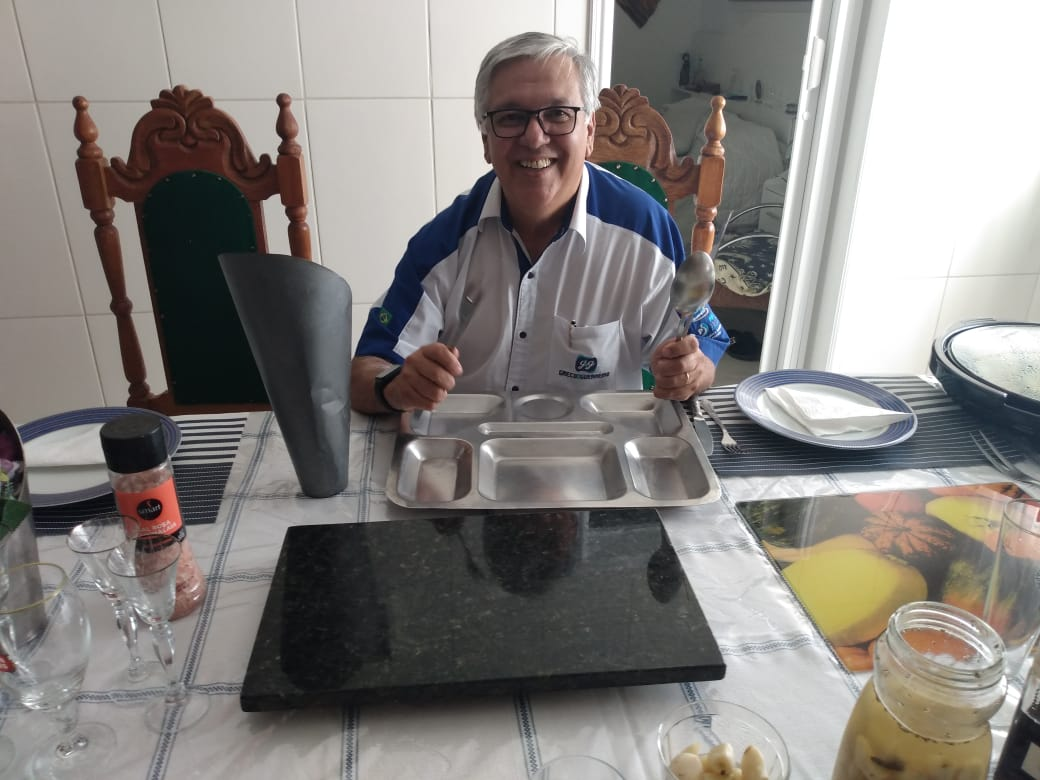
\includegraphics{Imagens/ZeAntonio.jpeg}

\textbf{O Zé Antonio filando uma boia na casa do Carlinhos da Marvina}

O Zé sempre esteve ligado aos nossos acontecimentos sociais e sempre
manteve contato comigo e com o Tomaz principalmente mesmo depois de se
casar e morar em Itatiba. Hoje mora em Campinas, casou-se com a Helena,
em segundas núpcias e está para se tornar o dono da cidade de Indaiatuba
onde está tocando um grande empreendimento na área de loteamentos
residenciais. Frequenta nossos encontros anuais, os encontros realizados
anualmente pela Nice do Correio com suporte do casal Tomaz e Célia. Do
Zé herdei e uso muito a expressão: \emph{Mas eu não brinquei}
principalmente quando minha mulher me pergunta se eu vou tomar banho. O
Zé conta, que quando era criança, à noitinha a mãe chamava:\\
-Minino, vem tomá banho pá jantá. Ele na maior cara de pau:\\
-Mas eu não brinquei.\\
Ou seja, não precisaria do banho porquê não brincou. Desculpa
esfarrapada que não colava com a mamãe severa:\\
-Já tomá banho vagabundo.

\section{A kombi do Seu Olézio}\label{a-kombi-do-seu-oluxe9zio}

A Kombi do Seu Olézio virou quase uma instituição em nossa cidade. Seu
Olézio que chegara como funcionário da Coletoria de Impostos, chegou à
cidade com numerosa família e certamente em condições financeiras
precárias pois um funcionário do Estado não tinha proventos lá muito
atraentes. Mas, muito esforçado, estudou, prestou concurso para Fiscal
de Rendas do Estado. Ou seja um funcionário mais graduado ganhando pela
média da produção dos outros colegas, mesmo depois de aposentado. Meu
irmão Delfino também foi Fiscal de Rendas e há mais de vinte anos seu
salário variava entre 12 e 15.000,00 reais. Seu Olézio, além de
construir uma casa enorme para acomodar a imensa prole, cuja
característica marcante e inovadora para nós, era uma já citada mesa
redonda com um sobre disco de madeira rotatório, com menor diâmetro, que
girava sobre a base da mesa movimentando os pratos sem que se precisasse
levantá-los. Adquiriu também uma Kombi, com lotação para 10 pessoas.
Como trabalhava em São Roque, para onde se deslocava todos os dias,
criou uma freguesia cativa, que embarcava de carona na Kombi. E ele
adorava isso e já ia fazendo paradas onde sabia que alguém precisava de
carona. A Maria Elisa do Dito Frango reservou-se o direito de sentar no
primeiro banco, na janelinha e ai de quem ousasse querer tomar seu lugar
no trono. Dava carona para estudantes, trabalhadores, policiais
militares que trabalhavam em Sorocaba ou São Roque e vivia lotado. Êle
dirigia cantando, rindo e conversando bastante, animadíssimo com o seu
público cativo de quem nunca cobrou ou aceitou um tostão. Adorava fazer
aquilo. Essa Kombi também serviu para nossos deslocamentos em bailes
pela região e o motorista era o Degas aqui, que era o único que tinha
habilitação. Também, os outros da turma eram todos menores de idade. Uma
vez fizeram uma viagem a Santos, na casa do Magrão, cunhado do Zé
Antonio. Dessa eu não participei. O Hélio do Ditinho Mandu e da
Wardomira, meteu a mão no chuveiro e levou um choque 220 V que abriu a
mão dele.

\section{A kombi do Nezinho}\label{a-kombi-do-nezinho}

O Nezinho era um barbeiro, que tinha um salãozinho mais ou menos onde
está o escritório de corretagem da Gizele, irmã do Zeca do Fuade. Pessoa
muito simples, meio envergonhado, falava pouco. Contratamos o Nezinho
para nos levar para Pilar do Sul, em um daqueles bailinhos. Mas o
motorista, por insegurança ou cuidado excessivo com o veículo dirigia
muito devagar. No máximo 40/50 km por hora e os gozadores começaram: Mas
Pilar é longe não, disse o Cláudio do Mirão. O Paulo do Olézio
respondia: É longe mêmo não?. Silêncio. Outro gaiato procovocava de
novo: Mas Pilar é longe não? Mas de nada adiantou. A viagem levou mais
de duas horas. No caminho ainda paramos para roubar mexericas mas fomos
surpreendidos com tiros para o alto.

\section{O impala do Paulo Padeiro}\label{o-impala-do-paulo-padeiro}

O Paulo Padeiro, marido da Dona Nena, pai do Paulinho, da Elizete e do
Nenê tinha um Chevrolet Impala lindo, \emph{rabo de peixe},
conservadíssimo, carinhosamente chamado de marraconada, pois só dava as
caras aos domingos. Mantinha o carro numa garagem nos fundos da casa,
anexa à Padaria Nossa Senhora Aparecida. A saída da garagem era pela rua
dos fundos, onde ficava a Caixa Econômica Estadual, depois Banco do
Brasil, originalmente o cinema do Neto. Os documentos ficavam guardados
num bufê na cozinha, dentro de um saco vazio de pó de café São Bento
(eita memória boa hein?). Na pracinha começava a operação \emph{Rouba
Impala}. O Paulinho entrava na casa e disfarçadamente afanava os
documentos. Depois ia pros fundos e destravava o portão para nós
entrarmos \emph{na miúda}. O Nenê, apesar de não ter carta, era exímio
motorista e tirava o Impala, quase raspando na parede do lado esquerdo.
O Paulo, talvez desconfiado de alguma arte, estacionava o carro grudado
na parede e saía pelo lado direito. Colávamos na parede, um na frente e
outro na traseira orientando o Nenê para tirar o carrão que saía rente
com a parede, quase um fio de cabelo da mesma. Operação delicada, pois
não podia acelerar para não despertar a atenção lá dentro da casa. O
Nenê assumia o volante e íamos \emph{no cacete} prá Pilar ou Araçoiaba.
Eu ia na frente, como motorista de plantão. O plano era: se algum
comando nos parasse eu desceria \emph{vomitando as tripa} e dizendo que
estava passando mal e que o Nenê, menor de idade e sem habilitação iria
me levar para o hospital. E a gente acreditava que isso funcionaria.
Santa ingenuidade. Tempos depois o Nenê já habilitado deu uma carona prá
minha mãe levando-a para Sorocaba. Minha mãe entregou para a Dona Nena:
*Ai, que delícia, fui de carona prá Sorocaba com o seu filho: o carro
parecia que ia voar``. Dona Nena, brava, pegou o Nenê de jeito: \emph{A
Dona Marvina disse que você foi vuando pá Sorocaba, dirigindo que nem
lôco}. E o Nenê me contando que minha mãe tinha entregue ele direitinho.
Coitada, era apenas força de expressão, pois acho que poucas vezes na
vida tinha andado num bólido daqueles.\\
Numa dessas \emph{roubadas} o Jonas do Vito Moraes, morrendo de ciúmes
porquê nunca era chamado a participar virou a cidade, à noite,
procurando um cadeado para trancar a garagem e estragar a nossa
brincadeirinha que já estava se tornando usual.\\
O Zé Antonio (Verinha) lembrou que o Paulo comprou um Maverick lindo
também, naquela cor entre o verde e o azul, que a Elizete usava para dar
infindáveis voltas pelas ruas do centro de Salto, todo domingo depois do
almoço. Meu sonho de consumo quando comecei a ganhar uns bons trocados,
trabalhando na região de Cascavel, no Paraná, era um carrão desses. Vim
de lá com um cheque visado de uns 30 mil cruzados para comprar um
Maverickão GT 1.8. E queria branco ainda. Meu irmão Crizólito tirou da
minha cabeça e me empurrou um Ompala duas portas, vermelho. Usadão mas
imponente. Tinha um toca fitas sem botões: tinha que virar o dial
\emph{no pino}. Uma vez saindo de Céu Azul rumo a Foz do Iguaçu, divisa
com Paraguay, viagem de 150 km. mais ou menos deu um problema no
trambulador e a alavanca de câmbio ficou \emph{boba}. Tive que voltar a
Céu Azul, 50 km mais ou menos, na segunda marcha, a 20 km/hora.\\
Queria um Maverick zero bala e me empurraram um Opala usado.

\section{Vito Moraes}\label{vito-moraes}

O Vito Moraes foi parte intrínseca do folclore de Salto de Pirapora. Era
tio do Zé Quito, pai do João do Vito que casou com a Mileide, e do
Jonas, Roberto, Ademar etc etc e bota etc nisso. Tinha uma carroça e com
seu cavalo catava tudo que é tralha que achava para comprar. Já me
chamaram de Vito Moraes pois adoro catar umas tranqueiras usadas nos
ferros velhos também. Tudo que você procurasse usado o Vito Moraes ou
tinha ou sabia onde encontrar. Homem simples, mas bom de conversa, sabia
contar uns causos e com isso ganhava a simpatia de todo o mundo. Certa
vez eu procurava arame farpado usado para arrumar umas cercas no sítio
da Fazendinha, onde eu brincava de boiadeiro. A quem recorrer? Fui no
Vito Morais: \emph{Carlinho, sei de um hóme lá pas banda do bairro dos
Barro que dismanchô umas cerca e tem um monte de arame véio pá vende}.
Botei o Vito no meu fusca e fomos atrás da mercadoria. O interessante
disso tudo foi o diálogo com o dono da mercadoria. O Vito chegou com a
prosa macia de quem quer comprar e pagar barato. Logo ofereceram aquele
café típico de sítio: bem fraco e bem doce, uma copada e tanto que levei
meia hora enrolando prá engolir. Aí começou a prosa: Eh aí nhô Joaquim
como é que tá a vida no sítio? Tem lidado c´as prantação? E o gadinho tá
engordando? E os fio como é que tão, são bão poceis? Ói, nhô Vito, o
Zezinho, mais véio, tá cum dizenove ano agora. Mais, pense num rapais
bão. O Zezinho \emph{num tem artura de bão}. É bão demais da conta. E o
João, mais moço, é pareio de bão, é bão pareio*. E nessas conversas,
intercaladas por goladas de café fraco, doce e frio a prosa ia
desenrolando e o Vito levando a conversa pro lado que nos interessava:
pechinchar e comprar barato.

\section{Sorocaba: a turma do Estadão - primeira
fase}\label{sorocaba-a-turma-do-estaduxe3o---primeira-fase}

Como já contei, fui estudar no Estadão em Sorocaba. O Instituto de
Ensino Júlio Prestes de Albuquerque (IEJPA), clik
\href{Imagens/Estadao.MP4}{aqui} para ver um filme, na Avenida Eugenio
Salerno, na mesma avenida do Seminário e da Escola Municipal. Era
naquela época, por volta dos anos 60 e durante as décadas seguintes, uma
instituição de peso em matéria de ensino em Sorocaba. Para entrar no
Ginásio, tinha que prestar um exame de Admissão, dificílimo. Eu, por
exemplo, bombei no exame de admissão, apesar de que tinha sofrido um
corte no dedo médio da mão direita \emph{brincando de pais} na
construção do cinema do Neto. Tinha dificuldade até para escrever mas
não é isso que justifica ter \emph{levado pau} no exame seletivo. Fui
para a OSE, Organização Sorocabana de Ensino, na rua da Penha perto da
Padre Luiz, onde cursei a primeira série. Na segunda série pedi
transferência para o Estadão, tendo dessa forma driblado o difícil exame
de admissão. Nessa época estudei com o Gilson Luchesi Delgado, filho do
dono da banca de jornais da praça Coronel Fernando Prestes, no centro de
Sorocaba. O Gilson é hoje um oncologista de renome na cidade. Tinha
também os filhos do Carlos Pinto: o César e o Carlos, que tinha um
defeito na perna e eu, maldosamente, o apelidei de Manco Capac, um
personagem do reino dos incas. Já praticava o bullying sem saber. Mas
era de uma forma carinhosa. O Carlos Pinto era advogado do Banco do
Brasil e tinha uma belíssima mansão no largo Nove de Julho, perto da
Casa das Mães Solteiras e convidado para estudar com os meninos,
desfrutei de grandes cafés e almoços. Na turma tinha também um cara
muito engraçado, chamado Ernâni, que depois descobri ser meu primo em
primeiro grau. As nossas mães, irmãs de sangue, não se davam e a mãe
dele recusou seu pedido de me levar na casa deles. O Ernâni, me lembro
muito bem tinha o número 18 e na chamada da aula de religião tínhamos
que responder Salve Maria. Número 1, Salve Maria, número 2 Salve Maria,
número 17 Salve Maria. Número 18 e o Ernâni gritou alto e bom som:
\emph{Viva São Pedro}. A classe explodiu, o Ernâni foi expulso e tomou
um zero de presente.\\
Nessa época o Estadão tinha um time de futebol de salão que ganhava
todas. O nome do time era: FuraGuerraMoaReiNelBron. O goleiro era o
Foramiglio, depois o Guerreiro, o Moa, filho do seu Moacir Pires de Melo
(este merece um capítulo especial), e da dona Lourdes, irmão da Regina,
casada com o José Maria Rosconi, da Helena, da Inês, do Pedrão e do
Tadeu. Rei, era o Reinaldo, pai do Reinaldo do RPM, de quem me tornei
grande amigo de tênis 40 anos depois. O Nelson e o Brondi completavam o
timaço de craques. Os campeonatos na quadra do Estadão eram vibrantes
tanto em matéria de bola como de espectadores e torcidas.\\
Famoso nessa época era o Bachir, um turquinho baixinho e briguento. Todo
dia ele arrumava uma briga, que era combinada para depois das aulas num
campinho em formato de cuscuzeiro, no fundo do vale, mais ou menos na
direção dos fundos do clube Ipanema. A gente tinha que descer um
barranco, atravessar o valo e subir para o campinho. No intervalo das
aulas já começava o buxixo: Vai tê briga, hoje tem briga. O Bachir
chamou fulano pro pau. Contendo a expectativa esperávamos \emph{dar o
sinal} do fim das aulas e saíamos correndo ladeira abaixo para não
perder a briga.\\
Dos professores o mais folclórico era o Professor Eglas, de Geografia,
famoso por ser irascível e perdulário na hora de dar notas. Era um tipo
assim visionário. Costumava dizer que o brasileiro só pensava em
futebol. Que se déssemos uma bola amarrada na ponta de uma vara o
brasileiro iria chutando essa bola, atravessar o mundo sem pensar em
mais nada. O Eglas tinha uma Romisetta. Talvez o Romi seria um
referência à Roma e Isetta o nome da fábrica, era um veículo para uma só
pessoa, em perfeito formato de ovo, sendo que a porta abria para frente,
deslocando o volante junto, tipo abertura de uma geladeira e não como a
abertura de portas laterais nos veículos convencionais. Seu Eglas era
tão odiado pelos alunos que, uma vez alguns se reuniram e levaram para a
escola sacos de esterco de vaca e encheram o Kinder Ovo (coisa que se
tornou moda mais de vinte anos depois) com: \emph{bosta de vaca}.
Contava-se que quando ele abriu a porta, que escancarava para a frente o
esterco foi despejado em cima dele. Não vi e não posso provar.\\
Quem mandava no colégio era dona Dulce Pupo, esposa do Dr Mussi, mãe do
futuro arquiteto Mussinho. Mas o diretor era o Seu Roque mas dizia a
lenda que dona Dulce ao flagar o Roque com uma funcionária na sala da
Diretoria, deu um golpe branco e passou a dirigir a escola com mão de
ferro, com o beneplácito do silenciado e culpado Roque. Ouvi dizer que o
Roque acabou até assumindo a tal secretária, cujo nome vou declinar por
motivos óbvios. Lembro-me do nome mas só revelo sob tortura. Nunca se
sabe.\\
A falar sobre o Estadão, não podemos esquecer do professor de francês
Victor Stroka, e do mestre de Matemática Edson Campioni.

\section{O Dito Frango}\label{o-dito-frango}

O Dito Frango foi daquelas figuras folclóricas que marcaram sua
onipresença em quase todos os acontecimentos cotidianos de Salto de
Pirapora. Tinha esse apelido por ter pernas compridas, como os frangos
caipiras. E era bom prá correr. Com mais de cinquenta anos participou de
um jogo de futebol no campo dos Parados e quando lançaram uma bola na
ponta esquerda, ele saiu em uma \emph{carrêra lôca} que não viu a mureta
que cercava os limites do campo. Literalmente voou por cima da mureta e
se levantou do outro lado todo faceiro e voltou pro campo. Aos mais de
80 levantava a perna e pulava por cima do sofá, conforme contou o Dito
Simprício, que carinhosamente apelidei de Chico Bento. Também se comenta
a sua virilidade mesmo com essa idade. Conta o Naile que ao mostrar
filmes picantes, o Dito ainda \emph{armava o circo}. O Frango também
teve uma prole numerosa: Nego (tocava trombone na banda e nos
conjuntinhos carnavalescos), Marilisa, Sid Conde (figuraça) o Canecão
(outra figuraça), o Ditinho (uma comédia de loucura), Magali e Adilson
Franguinho com quem pratiquei muito bullying. Hoje é muito meu amigo e
toda essa molecada que nós judiamos parece que perceberam que todas
aquelas gozações não eram maldade. De uma certa forma os incluíamos nas
rodas dos mais velhos mesmo que fosse prá fazer judiação. O Dito Frango
sempre marcou presença na praça, porquê morava ali perto e dessa forma
estava por dentro de tudo que rolava por ali. Muito me surpreendeu um
dia quando, falando com seriedade me disse: \emph{Carlinho, você foi o
número um no Sarto pá cuidá da famia}. Eu, entre surpreso e orgulhoso,
falei: Mas Dito, como você sabe disso? você não frequenta minha casa,
não sabe o que se passa ali. Me respondeu: não precisa, sentado aqui na
praça eu vejo você passar de carro levando sua mãe, depois o pai ou o
Luiz pros médicos, cuidando sempre deles. Confesso a minha comoção com o
seu senso arguto de observação do seu ponto predileto no centro: na
soleira da antiga barbearia do Romãozinho, hoje a loja do Bachar. No seu
aniversário de oitenta anos lhe dei uma botina de presente que ele
exibia todo orgulhoso, no seu posto de observador geral da república de
\emph{Sarto de Pirapora}.

\section{O Paulo e o Elía Turco}\label{o-paulo-e-o-eluxeda-turco}

A loja dos dois \emph{brimos} era perto da fonte, onde foi o Bradesco
por uns tempos e era mais voltada para a moda para cavalheiros e
senhoras. Vendiam sapatos, coisa que só se encontrava em Sorocaba na
época, roupas e até fogão à gás. Era como se dizia uma loja de
armarinhos. O Paulo era \emph{mais bão de lábia} e o Elias mais contido,
mais sério. Numa ocasião o Paulo chamou o Galo e anunciou: Trouxe um
blusão especialmente de São Paulo, peça única e exclusiva. O Galo, que
tinha ganhado esse apelido do Dirceu Sebo, por andar sempre meio
empombado, de peito estufado, querendo ser único e exclusivo comprou e
saiu desfilando todo garboso. Era uma blusa tipo moleton (esse nome
ainda não existia) nas cores cinza e branco, muito bonita. O Galo se
sentia \emph{o cara} como se diz hoje. Mas qual a surpresa e a decepção
ao descobrir que o Zorro que \emph{lombiava} latões de leite para o
Wilson Leiteiro também estava usando um igual. O Zorro era um
\emph{pinguço} que quando sóbrio fazia esses bicos prá comprar a
cachaça. Era um bom homem mas para o Galo usar uma blusa igual à que o
Zorro usava era o fim do mundo. A esperteza do Paulo Turco pregou uma
peça na pose do Galo. Tiramos muito sarro dele na época.

\section{A turma do Estadão - segunda
fase}\label{a-turma-do-estaduxe3o---segunda-fase}

Depois de tentar a vida em São Paulo, nessa fase de ginásio, e ser
jubilado de um dos melhores colégios estaduais da Capital: o Fernão Dias
Pais no bairro de Pinheiros, enfiei a viola no saco e voltei prá vidinha
de Salto. Como já contei trabalhando no Matarazzo o chefão Vilmos Toth
conseguiu viabilizar o transporte, um jipinho Willys amarelo dos anos
50, e voltei ao velho Estadão da Eugenio Salerno para concluir o ginásio
(terceira série em diante) e entrar no Científico. Para estudar à noite
em Sorocaba ainda não havia o ônibus dos estudantes. No Estadão tinha
uma turma da pesada. O diretor da noite era o Edson Campioni, professor
de Matemática e os outros mestres: Hugo Polo de Biologia, Horácio Reis
(pai do Júlio Reis Imóveis), um chato que me deu um zero redondíssimo, o
Toninho de Física, o Ivan de Química, Nelson Guedes, Rubens Cutter e por
aí afora. A turma da pesada: Ilson Alcoléa, Mauro Tadeu Moura, Adilson
Segamarchi, o Pintado, Nambuzinho etc. O Mauro teve uma passagem
fantástica. Achava que o professor o perseguia. Deixei ele colar uma
prova inteirinha minha, de tanto ele me encher o saco, cutucando da
carteira de trás: Carlinho mostra a prova, e eu morrendo de medo de
sermos pegos e eu tomar zero. Colou tudo que queria. Na hora de ver as
notas eu tirei 8,5 e ele ZERO. Ficou louco, queria brigar com o
Professor e eu pedindo para esperar para ver as provas. Primeiro o
mestre falava as notas, vinham as críticas habituais, normalmente
chamando os alunos de burros, o que naquela época podia: ainda não era
bullying e só depois entregava as provas. E eu: espera para ver as
provas Mauro e ele falando em perseguição: como pode eu copiei a prova
todinha, igualzinha a sua? Finalmente recebemos as provas em mãos. Fomos
conferir. As questões eram de forças resultantes e no final de cada
exercício tinha uma continha tipo: 4 vezes zero, 2 vezes zero etc. E o
Mauro colocou os resultados: 4 vezes zero igual a 4, 3 vezes zero igual
a 3. Eu disse: Mauro, o zero anula o produto e 4 vezes zero é zero e
assim por diante. Porquê você não colou o resultado? E êle: quando vi
aquela continha fiquei com vergonha de copiar o resultado e resolvi
fazer a conta eu mesmo. Deu no que deu. Passou a vontade de bater no
professor. E olha que o Mauro era briguento: encarou caras muito maiores
que ele por várias vezes.

\section{O Suva, meu primo de
Sorocaba}\label{o-suva-meu-primo-de-sorocaba}

O Suva, nascido Salvador, era meu primo. Faleceu há uns dois anos atrás.
Filho mais novo de família muito pobre. Meu tio Miro, irmão da minha mãe
Marvina, tinha sido ajudante de carreiro de boi do meu pai e segundo ela
contava quando passava pela cidade tinha que se proteger em cima do
carro de bois pois de tanto jogar pedras nos cachorros da rua, os cães
já o conheciam e o perseguiam. Ao completar idade resolveu servir o
exército para tentar tomar um rumo, talvez seguir a carreira militar.
Mas numas andanças na região de Barra Bonita, conheceu a Tia Lídia na
cidade de Igaraçu do Tietê: mocinha nova e muito bonita, na flor dos
dezesseis anos e ele se apaixonou perdidamente. Mas já tinha se alistado
expontâneamente no exército e foi chamado para servir. Naquela época era
obrigado a servir o exército com dezoito anos mas, se ao se apresentar
se você se declarasse agricultor era dispensado do serviço militar, como
se dizia. Mas ele insistiu em se alistar, se apresentou e depois
desistiu de servir e virou um \emph{desertor}. Casou-se com a tia Lídia
mas viveu escondido sem nem poder fazer casamento de papel passado e nem
registro da penca de filhos que foram nascendo. Poderia a qualquer
momento ser preso por ter desertado. Uma espécie de traidor da Pátria.
Só foi registrar os filhos depois de grandes, quando a sua deserção
caducou ou caiu no esquecimento. Tiveram os filhos João, que virou
pescador no rio Tietê, o Milton e o Zé que viraram pedreiros em
Sorocaba, as filhas Clair, Benê, Ornélia (homenagem à minha avó
Dornélia) e a Verinha que ficou muito conhecida em Sorocaba por ser dona
da loja Shoppig Seven na galeria Santa Clara na Padre Luiz e depois no
shopping Sorocaba. Por último, a raspa do tacho: o Suva, criado com
\emph{todo o leite}, na condição de caçulinha. Nunca estudou e nem
trabalhou. Com o sucesso da Verinha que ao comprar a loja de importados
do Ary Proença deu como parte do pagamento a casa dos pais, o Suva,
talvez por esse motivo ou pela caçulice mesmo se achava no direito de
ter tudo sem trabalhar. A Vera comprou um fusca para êle que quando ele
veio num baile em Salto caiu a roda. Exigiu toca fitas, o must da época,
rodas de tala larga etc até comprar um Dodge Dart branco com o qual
participava de rachas com os boyzinhos endinheirados de Sorocaba. Só que
quem bancava os estragos dos rachas e cavalos de pau era a irmã. Tentou
até montar uma loja de jeans para ele, na própria galeria Santa Clara
mas ele nem aparecia para abrir ou tomar conta da loja e ela se
desdobrava nas duas. Sempre foi muito trabalhadora e excelente
comerciante. Aí resolveu se casar para ver se botava um freio nas
investidas do Suva. E se casou com o Luizinho, também metido a boyzinho
e igualmente durango. Numa ocasião no bar Balaio pediu a moto do Tomaz
emprestada para dar uma volta e levou uma semana para devolver. Ficou
curtindo e se exibindo para as gatinhas. Quando conheceu a Vera era
vendedor da Móveis Gonçalves, loja muito famosa e que fabricava ótimos
móveis dos quais tenho um exemplar. Mas aí, como se dizia em Salto:
jogaram o sapo na água. O Luizinho largou a carreira frustrada de
vendedor de móveis, tirou o catálogo de móveis de debaixo do braço e
assumiu com \emph{A} maiúsculo os negócios da Vera, que por sinal até
ali ia muito bem: tinha uma bela casa na Paes de Linhares na Vila Fiori,
sempre um bom carro e uma coleção de sapatos à \emph{la} Imelda Marcos.
Maldade minha: Imelda Marcos mulher de Ferdinando Marcos, ditador
deposto das Filipinas devia ter uns 2.000 sapatos, a Vera só uns 200. O
Luizinho assumiu os negócios mas não tinha tino nem simpatia e quis
inovar entrando no negócio de troca de dólares. Tentou uma sociedade
frustrada numa fábrica de tanques com o Alfredo Galán, filho da dona da
casa das velas e afins, na rua Padre Luiz vizinha do Mercado Municipal
de Sorocaba. Aí a coisa se degringolou de vez e o sucesso da Vera foi
virando suco (referência à loja de sucos de frutas na Paulista chamada o
Engenheiro que virou suco). Perderam casa, loja e também se separaram.
Uma grande lástima pois a Verinha tinha muito tino comercial, sabia
cativar. As mulheres mais ricas e poderosas de Sorocaba (muitos homens
também) eram clientes fidelíssimos dela. E no meio dessa epopeia toda o
Suva, sempre frequentando os melhores locais e companhias de Sorocaba:
Kana Kauê, Tribeca, Soft e sempre falando com sotaque muito caipira. Se
virava fazendo bicos como vendedor de carros para amigos como Marquinhos
da Komida e outros. Chegou até a ser sócio (ou apenas chamariz?) de uma
discoteca famosa em Sorocaba há uns dez anos atrás: a Aplle. Largou tudo
pois me disse que não aguentava varar madrugadas no empreendimento. Na
verdade gostava mesmo era de dormir e não ter compromisso com nada.
Acabou morrendo sozinho quando estava feliz por ter adquirido uma
pequena chácara onde sonhava lidar com as criações de que sempre gostou.
Chegou a ter uma avícola nos altos da Nogueira Padilha mas não durou
muito tempo. Quando se separou da Ivete a loja teve fim precoce. Mas,
marcou época nas noitadas e nas rodas de motociclistas dos riquinhos
sorocabanos, mesmo sem sê-lo. Sempre andou no meio de gatinhas e
mulheres bonitas. Tinha o seu \emph{charme caipira} e agradava.

\section{A kombi do Elia Gelo}\label{a-kombi-do-elia-gelo}

O \emph{Elía gelo}, na verdade Elias Canalle, tio da Magali Canalle
tinha uma Kombi de aluguel, que se soltasse na descidão da ponte já ia
parar na zona em Sorocaba. Ele próprio era freguez de carteirinha da
\emph{terra vermeia}. Levou muito a nossa turma para os bailes das
redondezas e era um cara que além de meio louco, era gozador e
engraçado. Um vez inventou de descer com a Kombi pela rua do centro
engatada em primeira e com um tijolo no acelerador: quando chegou perto
do bar do Tonico (hoje Cochinha) desceu da Kombi, correu no bar, tomou
uma pinga no balcão e voltou prá Kombi que descia engasgando e dando
tranquinhos. No Carnaval retirou todas as portas da Kombi que se
transformou numa mini jardineira. Acontece que nesse carnaval vieram uns
negros fortes do Cafundó, encheram o latão e prá variar arrumaram briga.
Chamaram o \emph{Mário Sordado}, pai do Paulinho Mixirica que não tinha
medo de entrar no meio de qualquer briga e \emph{descer o cassetete
parêio}. Um deles era o Levino, negro forte e encrenqueiro lá da turma
do Guaxinduva. Quando viram o Seu Mário entortar o quepe de lado e
empunhar o cassetete já foram \emph{mijando pá tráis}: \emph{Não Seu
Mário, nóis arrespeita o sinhor}. Não tinha viatura para levar os
briguentos para a delegacia e o Elias, que quando viu a coisa engrossar
chamou a polícia, correu buscar a Kombi para fazer o translado. Só que
tinha tirado todas as portas para a farra do Carnaval e então os presos
eram jogados dentro da Kombi e saiam pelo outro lado e desapareciam.
Resumo da operação: ninguém foi preso.

\section{\texorpdfstring{A turminha da \emph{Via Sacra} e do
\emph{Curto}}{A turminha da Via Sacra e do Curto}}\label{a-turminha-da-via-sacra-e-do-curto}

Galo, Nazírio, Zé Carlinho, o Degas aqui e outros tantos gostávamos de
ver a saída do culto da Igreja dos crentes perto da fonte. O Nazirinho
falava: \emph{Vamo vê a sortada do curto}. Era a saída do pessoal da
igreja e a gente queria flertar com as crentinhas. Mas a preparação
começava no bar do Feliciano tomando umas geladas e o propósito era
beber em todos os bares até chegar no Boqueirão, no começo da estrada do
Matadouro. Bebemos no bar do Chico Faca, no do pai do Mosquito, no bar
do Izídio, pai do Bolinho e por aí acima. Do lado do Izídio tinha uma
igreja crente bem simples, e nós entramos. Eu pedi a palavra, fui lá na
frente e fiz um discurso de louvação aos presentes e à minha crença
naquela religião que eu nem sabia de qual se tratava. Tudo no embalo da
\emph{mardita}. A \emph{procissão} continou e fomos terminar quase no
Campo Largo.

\section{O barracão do Batista}\label{o-barracuxe3o-do-batista}

Esse foi outro lugar em que bati ponto muitas vezes, quando o Batista já
meio \emph{caducando} passou o bastão para o Nego. Quem trabalhava ali
era o Cissão, o Gordo além do filho do Nego, que desde moleque já bebia
bem, tanto que um dia tomou umas pingas na Bertília e foi prá casa
tomando uma latinha e mastigando o saldo final de um \emph{baita
torresmo}. Deitou de roupa e tudo e dormiu mascando o couro: no dia
seguinte acordou com a roupa de cama toda engordurada. Cada um tinha
suas histórias peculiares: O Nego tinha um cliente que era a fazenda
Frutolândia e o Cissão sempre ia lá buscar ou levar cereais. Um dia
chegou pro Nego: \emph{A turma do Frutulano num qué vendê o fejão}. E o
Nego: Quem?. O Frutulano. Quem é esse?. \emph{Aqueles hóme da fazenda de
fruita}. Era a Frutolândia. O Gordo era um moreno baixote pesando uns
140 kilos e eu zuava falando que no baile as mulheres não queriam dançar
com êle porque não dava prá \emph{abracar}, corruptela de abraçar,
devido à circunferência da cintura. Uma vez foi no centro de Sorocaba e
ficou preso dentro do elevador que subia e descia, subia e descia e ele
não sabia como sair lá de dentro. Quando o Nego mandou o caminhão para
buscar umas coisas minhas em São Paulo quem diz que o Gordo entrava no
elevador. Subiu 14 andares à pé: \emph{nessa bosta eu num entro}. Quem
já andava pelo barracão do Nego era o Telmo, hoje arquiteto da
Prefeitura. Tinha uns 9/10 anos, rechonchudinho, calça curta, curioso e
louco prá entrar na conversa dos mais velhos. E a gente judiava dele:
sai prá lá gordinho curioso, \emph{o que tá querendo escuitá}. Ele saia
meio sem graça mas logo estava de volta e acabamos incorporando o
Gordinho na roda.

\section{Zé Martim}\label{zuxe9-martim}

Pense num \emph{hóminho} chato, \emph{pidonho}, \emph{putanhêro} e
entrão. Vendia leite de porta em porta e quando a dona da casa era
bonita já ia entrando e ia parar na cozinha. \emph{Óia o leiteeeee} num
grito ardido e esganiçado que assustava as mulheres, que muitas vezes
nem vestidas direito estavam. Uma vez mandei fazer uns cochos de
canafístula, uma madeira danada de dura prá aceitar um prego. Era para
tratar do gado \emph{no coxo}, por falta de pasto. Ele chegou, coçou a
cabeça jogando os poucos cabelos para o lado e mandou: Porquê num dá os
coxo prá mim. Mandei ele pastar. Ele morava perto do sítio da Mulatinha,
depois Romãozinho e seu vizinho Otacílio, que era irmão do Newton
Guimarães, prefeito na época convidou o governador José Maria Marin para
um jantar no sítio. O \emph{ladrão de medalhas das Olimpíadas} chegou
com o seu séquito de puxa sacos e o Newton respectivamente, entre os
quais a linda médica Regina Caramuru, mulher alta, de presença e de um
humor fantástico quando recebia cantadas: tirava de letra e deixava os
baixinhos como o Ziquinho da Prefeitura desenxabidos quando respondia
com altivez e classe: O que você quer Ziquinho, você é casado, é feio e
baixinho e ria gostosamente. Desmontava qualquer aventureiro. Acabou se
casando com o Ronaldo Moreno, da tradicional família de Sorocaba que
tinha a famosa loja de materiais de construção perto da ponte Maurício
Delosso, logo depois do largo do Canhão. O Zé Martins foi convidado e
vestiu a sua melhor roupa: calça de brim com listras de pijama e camisa
xadrez com os botões \emph{tudo fora de lugar}, ou seja pulando as
casas. Chegou, a comitiva já toda assentada, deu uma olhada geral e
soltou na sua voz estridente: \emph{Aquele brancão que é o hómeeeeeee?
Ainda bem que o larápio não ouviu pois estava todo entusiasmado com a
Regina Caramuru sentada estrategicamente ao seu lado. O governador
acabou de comer e a Marina, mulher do Newton, ou seja a primeira dama
saltopiraporense (kkkk): Coma mais }Dotôr\emph{, tire mais um pouco.
Não, Dona Marina, muito obrigado estou satisfeito, a comida está
deliciosa e todos aqueles salamaleques de político }mais liso do que
bagre ensaboado\emph{. E a Marina emendou: }Coma Dôtor, o que sobrá vai
jogá pos porco mêmo*. Consternação geral do bando de puxa sacos. Esse
era um ditado comum, uma brincadeira mas a Marina não se deu conta de
que não era adequada para a ocasião, se bem que no meu ponto de vista o
adequado seria escorraçar o safado com varas de malhar feijão. Para não
perder a deixa: José Maria Marin foi jogador de futebol mediano pelo
time do São Paulo mas muito esperto se meteu na política e como vice
governador na vacância do cargo assumiu o governo do Estado. Conta-se, e
disso não há provas, que nas suas militâncias políticas se apropriou da
bagatela de 5 milhões de reais que eram destinados á campanha de Jânio
Quadros. Passou no doador se dizendo autorizado a recolher a quantia
que, dizem, nunca chegou ao destinatário e, fala-se, comprou um
chiquérrimo apartamento na Alameda Franca no carésimo bairro dos Jardins
em São Paulo. O resto da história todo mundo conhece: meter no bolso
medalhas de ouro dos medalhados que ficaram sem medalhas e tomar prisão
em cárcere de ouro em pleno Rockfeller Center nos States.

\section{Jogo de bolinhas de gude}\label{jogo-de-bolinhas-de-gude}

Na calçada da Igreja, ponto privilegiado \emph{pá bisoiá} a vida que
escorria perguiçosa pela rua do meio se sentavam João Friage, Fonseca,
Guíche, Dito Frango, Zé Curinga, tudo \emph{debarde, à toa, tudo coçano
o saco}. Já tinham ido \emph{se lavá} e muitos tomado banho de rio no
Piraporão, na altura da ponte. Ou então no tradicional \emph{bacião de
fôia} com água esquentada no fogão de lenha e despejada de um canecão
também \emph{de fôia} (folha de Flandres). Quem fazia era o \emph{Gir
bicicretêro}, da Belarmino geralmente com latas de leite condensado e
congêneres. O Fonseca vestido com uma camisa amarela do tipo \emph{volta
ao mundo}, igual a camisa do Miguel do Paco, que rolou com ela na
fogueira. Ia chegando gente e a prosa aumentando. Chegou o Genorzinho
contando da aposta que fez de trocar as telhas da Igreja quando
(empiricamente) usou o princípio do pêndulo da Física, colocando dois
meios tambores amarrados em cada ponta de uma corda e passando por uma
roldana no alto do telhado. Enchia o meio tambor de telhas novas aqui
embaixo e o de cima com as telhas a serem substituídas e quando o peso
deste excedia o outro a carga que descia içava para o alto a de telhas
novas. Garanto que nunca tinha ouvido falar de Pitágoras ou Tales de
Mileto mas aplicou direitinho os princípios da Física. Ele no seu
português peculiar chamava a operação de \emph{guingorra} (gangorra). O
Genorzinho era louco por uma aposta. Apostou uma vez na venda do
Martinho (hoje bar do Ademir Pupo) quem acertava quantos postes tinham
até a Santa Casa. Um falou vinte, outro trinta e assim por diante. O
Genor falou: aposto que dá 26. Casaram a aposta e foram conferir.
Batata: 26 postes. O Genor tinha contado os postes antes de provocar a
turma na demanda. A prosa foi mudando de rumo. Passou o \emph{Orlando
Minêro} do outro lado da rua, na prosa com Romeu Marcelo e o João da
Barra. Na base da \emph{meia boca, bem por baxo do quieto}, a turma
comentou da briga do Távio Farrapo c´o Orlando Minêro. \emph{É, o Távio
arrastô pô Orlando, lavô mio, cavocô de vórta, sartô de banda}. Tentando
segurar o Orlando, homem forte, estavam o \emph{Antonho Árve} e o
Izidorinho, pai do Jura Banana: dois homens pequenos que não davam o
peso de um braço do Orlando que foi arrastando os dois pelo pedregulho
como se estivessem esquiando. O Orlando tinha uma casa grande, do lado
da antiga Prefeitura (a primeira ao lado do grupo Afonso Vergueiro),
onde tá hoje o Marcos de Barros. Tinha um monte de cachorro veadeiro.
Mais de trinta com certeza. Tinha também um monte de filhas bonitas,
umas morenas acobreadas e o Degas aqui namorou duas delas, a primeira eu
tinha uns 16 anos e a segunda eu já na faixa dos trinta e tantos. Por
falar em Romeu Marcelo, quando eu tinha uns 9 anos mais ou menos fui na
reza com a Mamãe e como era muito irrequieto dei uma escapada da igreja
e fui dar uma olhada no movimento da rua. Bem do local onde depois tinha
a banca de revistas do Zé Leite vi o Orácio, irmão do Jair Jacó, no meio
da rua com uma espingarda por detrás do corpo. A cena ainda está nítida
na minha memória: o Romeu abriu a porta da frente da casa, que na
verdade era cortada em duas partes e a parte de cima que servia de porta
e janela ao mesmo tempo, estava aberta. O Romeu estendeu o braço para
fora para soltar a tranca da parte de baixo da porta e saiu para a rua.
Nisso ouvi o tiro desferido pelo Orácio do meio da rua que atingiu as
partes baixas do outro. Corri assustado para dentro da Igreja de onde
minha mãe já vinha correndo para saber o que estava acontecendo. O Romeu
foi levado às pressas para Sorocaba e escapou dessa. Disseram depois que
a bucha da espingarda, daquelas de carregar pela boca, entrou junto com
a pólvora devido à curta distância que o tiro foi desferido. A causa
disseram que foi por adultério. E eram compadres. Vá saber!!!!!!!

\section{O cinema do Neto}\label{o-cinema-do-neto}

A antiga sala de espetáculos, como se gabava o Neto, era no local onde o
Júnior, neto do João da nhá Cota, montou a Pousada Santos, prá cima do
armazém do \emph{Zé do Santo}.Na verdade o pioneiro do cinema foi o
Vidal Marcelo que depois vendeu para o Neto, em parceria com seu tio
Zélão da Dorva, da turma da Nhá Cota. Anos depois o Neto construiu uma
sala nova onde está hoje o Banco do Brasil. Ali o Carlinho da Marvina,
\emph{brincando de pais} ou seja brincadeira de \emph{péga péga} rasgou
o dedo médio da mão direita quando pulou de um andaime daqueles feito de
pontalete e para não ser pego pulou do andaime, no escuro, e espetou o
dedo num \emph{baita prego caibrão}. Guardo a cicatriz até hoje pois
naquela época dar pontos nem pensar. Nem Santa Casa tinha. Era curativo
na farmácia do Seo Jaime mesmo.\\
No cinema novo, com tela \emph{palarâmica} como dizia o Jair Pato,
passava muita fita do Mazarropi, Zorro, Cavalêro Negro, Hopalong Casside
muito filme mexicano e como não podia faltar a Paixão de Cristo na Sexta
Feira Maior. O Neto convidava prá sessão: \emph{Vou exibir um filmaço
hoje em CinemasCope e Technicolor, com o Pedro Armendáriz}. O Neto era
dos poucos que falava com éle (e não erre) e usava o plural, pois era
professor substituto no Grupo Escolar. Freguês de carterinha dos
\emph{firme de farvest} eram o Curingão, o Tocha da Mariquinha e o Jura
Bálas de ovos. Chegavam a dar tiros na tela, com os dedos da mão
imitando um 38, prá ajudar o mocinho matar os bandidos ou os índios. O
Jura Bálas de Óvos tinha esse apelido, porque passava gritando com uma
cesta de \emph{páia}: \emph{Balas de óvos, balas de óvos} e como era
fanho a molecada imitava escondida atrás do poste ou da parede da igreja
e aí, \emph{sêbo nas canela}, porquê se ele pega, nem a banda toca.\\
Tempos depois \emph{no raiá dos ano setenta}, na plateia do cinema do
Néto toda a moçada de Salto presente: Noêmia do Neguito, Ilda do Vadô,
Cirley do Dito Coelho, Carlinho da Marvina, Zé Carlinho, a turma do
Romãozinho, Zé do lico, Galo, Querubim. O Dérfão tarado foi entrando no
escurinho, \emph{só sondano, por báxo do quieto, cum bandideza}. Mas
tanto as moças como o Zé Pilar já estavam \emph{de picinê} (pince nez)
no taradão, \emph{só de butuca} esperando o que ele iria aprontar. E não
é que ele tentou enfiar a mão por baixo da cadeira mas, a moça esperta
jogou o corpo prá frente e prendeu o braço dele que teve que assistir
quinze minutos de filme, arcado prá frente com o braço preso, doendo e
quietinho para não ser pego no flagrante. Dérfão virou sinônimo de
tarado em Salto. \emph{Aí, Dérfão, num pode vê muié?, tarado}. O Neto,
na verdade, era um cinéfilo só que, economicamente, era inviável ele
fazer uma programação de filmes mais culturais, cinema de arte etc.
Então muitas vezes ele trazia filmes desse naipe e fazia sessões para
convidados, geralmente na quarta-feira, quando o cinema nem abria para o
público. Era o Cinema Paradiso do Neto! De Bergman para cima.

\section{Jogo do time dos Parados nos
domingos}\label{jogo-do-time-dos-parados-nos-domingos}

Outro programa legal era descer para o \emph{campo de bola} nos domingos
à tarde antes no peladão do Bumbo e depois no Estádio Municipal,
praticamente exclusivo dos Parados. A terminologia das posições era
\emph{gortipa} (goal keeper) o goleiro, centroflôr (center for) era o
centro avante, furbéque, (full beck) era o béque.

\section{O time dos Parados}\label{o-time-dos-parados}

Depois veio o time dos Parados.

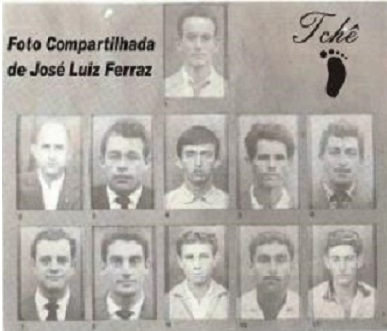
\includegraphics{Imagens/time dos Parados2.jpeg}

\textbf{O imbatível \emph{scratch} do final dos anos 1960}

Saiba que são os craques da foto, pela ordem:

\textbf{Mirto Pêxe} - goleiro - era um peixe de agilidade.\\
\textbf{Ataliba} - o do Armazém e da Igreja - Realizava até cerimônias
fúnebres na ausência do padre.\\
\textbf{Japão} - seu nome era o brasileiríssimo Moacir, mas a cara era
de japonês.\\
\textbf{Dorfão} - ou Gastão, como ele próprio gostava de ser chamado.
Filho do Argemirão da Belarmino.\\
\textbf{Laurinho} - Está vivo ainda. Já contamos que era o
\emph{mercenário da bola}.\\
\textbf{Cabo Jorge} - Também vivo. Pai do Jorginho e marido da Elza. Foi
um dos maiores briguentos dos Parados, junto com o Moacir Japão.\\
\textbf{Zito} - Elesbão Gonçalves, pai do Junick e do Roger.\\
\textbf{João Turco} - já contamos todo o seu \emph{folclorismo}.\\
\textbf{Lagarto} - Hábil driblador bem como o irmão Lagartinho.\\
\textbf{Butija} - meio de campo baixinho que \emph{cruzava} na medida na
cabeça do joão Turco.\\
\textbf{Jaiminho Vigorelli} - Era uma máquina de costura para driblar.

O time ganhou esse apelido porque formaram o time com os jogadores que,
por não gostarem da sistemática autoritária e impositiva dos dirigentes
compostos pelas famílias dos Marcelos, todos ruins de bola e pela
família do João da Nhá Cota, igualmente pernas de pau, pararam de jogar
e por falta de opção ficaram \emph{parados}. Alguém teve a ideia de
juntar esses atletas que no geral eram realmente os \emph{bons de bola}
e formar um novo time que por falta de idéia melhor ficou como
\emph{time dos Parados} mesmo e foi um sucesso. Extrapolou os estreitos
limites do futebol amador da época, tornando-se conhecido e respeitado
em Tatuí, Capela do Alto, Piedade e Pilar do Sul e outras tantas cidades
da região. Respeitados pelo futebol e por não temerem uma boa briga em
campo. O time foi comandado pelo Neguito e pelo Paulo Padeiro. Dos
cracaços que me lembro tinha o Nardo, goleiro, um gigante no gol. O
Botija irmão do Peixoto, excelente para fazer cruzamentos e alçar a bola
na medida da cabeça do João Turco, o terror dos beques e dos goleiros:
subia para escabecear a mais de meio metro da altura dos adversários e
ainda os cutucava, xingava e até passava a mão na bunda, quando o juiz
não estava olhando. Os beques eram o Ataliba (o do armazém e da igreja),
o Odair e o Furazóio. Meio de campo Cabo Jorge, encrenqueiro e
briguento, junto com o Moacir Japão, outro que adorava uma encrenca. O
centroavante era o Manezinho, que não era de Salto. Parece que veio do
Vau Novo onde o Matarazzo tinha uma unidade. Ponta esquerda Áureo (o
próprio, ex Bertilha) e depois o Edson Careca, filho do Zequinha
Barbeiro. Outros craques de fora também jogaram pelos Parados: o
Fernando de Boituva, funcionário do Bamerindus, o Gão de Sorocaba.\\
O Áureo não era exatamente um craque da bola. Jogava na ponta esquerda e
fazia bons cruzamentos na área sempre buscando a altura do João Turco. O
Áureo era mais famoso por ser uma figura folclórica, cheio de
maneirismos para falar inventando um vocabulário próprio. O João Turco
contava que quando precisou cortar um pedaço do cordão da chuteira que
estava incomodando parou o treino e perguntou: \emph{Alguém por acaso
tem um caniffs?????}. Ele queria dizer um canivete. Também sempre
contado ou inventado pelo João Turco quando o pessoal de Salto foi pela
primeira vez para a praia numa excursão montada pelo João do Vito, ao
chegar na represa Billings, ou seja a cerca de 50 quilômetros do mar o
Áureo desceu do ônibus com uma toalha nas costas cantando: \emph{Esse
mal (mar) é meu} crente que já estava na praia: nunca tinha visto o mar
e muito menos sabia da existência da represa Billings. O Laurinho dizem
que pedia dinheiro prá entrar em campo. Senão, tava com dor de barriga
ou com câimbra. Bastava o Paulo Padeiro acenar com uma nota de
cinquentinha na moeda da época que ele melhorava rapidinho. Tinha ainda
o Cabo Jorge, o Moacir Japão, os dois que não tinham medo de cara feia e
partiam prá porrada mesmo. Mais tarde o Japãozinho(Cipriano) e bem mais
tarde o Waldemar Picolé, Orlandinho , Flavinho (Deus que azude, tô
sastifeito), o Lagarto, grande driblador e o irmão Lagartinho. O Beninha
do Leonel, trabalhava na Cosipa e jogava também. Arrumou muita
\emph{ingrisia}. Chegou a dar uma cabeçada na boca de um juiz, extraindo
dele um dente que voou no gramado e o juiz catou na grama e exibia para
mostrar a agressão sofrida. O Beninha depois de ter uma falta marcada
tomou a bola nas mãos e se dirigiu ao juiz para, supostamente, entregar
a bola para ser colocada na marca da cobrança de falta mas, quando o
juiz foi pegar a bola, ele a tirou de lado e desferiu uma certeira
cabeçada, fazendo a extração sem anestesia. E olha, que o Beninha era
baixinho como eu. Imagine se fosse grande.\\
Na torcida tinha o Zé Padre, depois Zé Martelo no comando da
\emph{xingação} \emph{Vamo insurtá o juiz, esse larápio lazarento,
meneghete caiporento, ladrão morfético}. As moças também desciam para o
campo dos Parados, mas aí já existiam as arquibancadas de cimento, duras
mas tinha pelo menos onde sentar ao contrário do \emph{peladão} do
Bumbo, e ainda tinha a grama no campo, novidade alvissareira naqueles
tempos.\\
Uma outra esclação importante dos Parados: Nardo, no gol. Taliba, Fura
Zóio e Odair na defesa. Laurinho, Cabo Jorge e Butija, depois Nei do
Arardo no meio campo. Manezinho, João Turco dentro da área. Ponta
direita; Edson Careca. Ponta esquerda: Áureo da Bertília.

\section{O time do Bumbo}\label{o-time-do-bumbo}

O time do Bumbo, acho que tinha esse nome porque sempre apanhava, era
dominado pela turma do João da Nhá Cota: Dorival, irmão do Balaio,
jogador meia boca como o eram os Marcellos: Zé Carroça e Luiz Marcelo.
Eram também do outro lado da política. Mas abrigaram vários craques: O
Nê, briguento e bom de bola, o Coio também com as mesmas qualidades e
defeitos, o Cridão, de quem o filho Guelo do Trevão herdou as
habilidades debaixo dos três paus. O que matava era enxertar os chamados
\emph{grossos} enfiados guela abaixo pelos cartolas da época. Mas o
Bumbo também marcou época. E também eram donos do campo (se não me
engano o terreno era do João de Nhá Cota) e para jogar lá o time dos
Parados, via Paulo Padeiro, Marreco, Jair Pato tinha que fazer altas
confabulações para poder utilizar o campo. Nessa época os jogos eram
tratados. O Paulo Padeiro foi em Pilar tratar um jogo. Normalmente
levavam um guarda chuva. Daí a gozação com quem saía de casa com um
guarda chuva, mesmo sem sinal de chuva: Eh aí vai tratar jogo? Outros
craques do Bumbo foram o Peixoto e o irmão Butija, o Piranha, genro do
Orlando Mineiro, o Rodeiro (jogador mediano), irmão do Roderinho que
começou nos Paradinho.

\section{As Festas Juninas}\label{as-festas-juninas}

Festa de São João e Santo AntonIo eram programas divertidos também.
Armavam uma \emph{caieira} no meio da rua abaixo da Matriz, com lenha
trazida de carro de boi, doadas pelo \emph{Seu Gênor} ou algum outro
festeiro rico. Vinha a turma do Cafundó e a turma dos Florianos prá
cantar um samba. A pinga rolava e o improviso \emph{comia sôrto}. Lúcio
Camargo, Antonho Furquim, Pinhé eram bons de cantoria, tanto no
improviso ou nos versinhos inocentes já decorados. Do Lúcio ficou uma
pérola. Um refrão repetitivo e gostoso: \emph{Avoô i sentô, avoô i
sentô, no gáio da laranjêra, avoô i sento} e ia repetindo enquanto a
inspiração nãob vinha. O Lúcio Camargo gostava também de cantar \emph{A
Pombinha Branca}. Mais um gole da \emph{marvada, um táio no ingasga
gato} que podia ser um conhaque de alcatrão São João da Barra, ou
cachaça no mais das vezes e o repente surgia na hora. Tinha o leilão de
gado na mangueira do Gênor. Vicente de Nhá Cota, Vadô Mantino, Cascudo,
tudo querendo \emph{pegá umas rebarba barata}, João do Nísio, Nestorlão,
Calixtro (pai do Dirceu Sebo, do Dineu Lindóia, da Derli, e da Dircéia
do Rubatão), Nhô Norato com o paierão aceso,fumo macaio do bão, o Nhá
(Diunísio Leite, pai do Quinzão), o Nhô Vídio (bom de lida prá ajudar na
apartação) tudo trepado na última tábua da mangueira olhando os garrotes
e as novilhas doados prá festa. No meio um bezerro \emph{náfico} de uma
perna, ou uma vaca \emph{três teto} ou seja o descarte ia para o leilão.
Como era dado impurravam as \emph{tranquêra}. O litro de conhaque corria
solto, \emph{prá morde (autoria do João di Nhá Cota) de isquentá a
gargante do leiloeiro i garrá corage nos arrematêro}.

\section{A Procissão do Senhor Morto na Sexta Feira
Maior}\label{a-procissuxe3o-do-senhor-morto-na-sexta-feira-maior}

Era uma festa que juntava todo o povo: os curiosos para assistir, os da
paquera prá ver as moças bonitas. A procissão começava na Matriz, subia
pela praça da fonte, ia até a Caixa d´agua onde morava o Chico Branco e
voltava. Tinha altar na casa da Dona Áurea do Agenor dos Santos, na casa
da Dona Célia do Zé Martelo, na casa da Dona Antonia, mãe do Neguitinho,
na casa da Orídia do Dito Pão e assim por diante emulando as estações da
peregrinação de Cristo com a Santa Cruz. Numa delas tinha até a Verônica
que chorava e enxugava o rosto de Cristo. Eu, coroinha vestido de batina
vermelha e um roquete branco(espécie de sobretudo) seguia atrás do Padre
Boaventura Manara que puxava a procissão e atrás dele o andor com o
Senhor Morto, carregado pelos \emph{marianos}, homens paramentados com
roupas iguais e com fitas vermelhas no peito, previamente selecionados
pelo Padre. Seria a figura masculina das \emph{filhas de Maria}, que
também se paramentavam igualmente, todas de branco e com fitas azuis no
peito. Uma beleza. Ainda tinha acompanhamento da banda comandada pelo
Antonho Músico, pai da Toninha do Quinzão E o Degas aqui junto com os
outros coroinhas levando o sino para a cerimônia nos altares. Na altura
do armazém do Eugênio Seabra, pai do nosso amigo Levy, logo depois da
fonte este que vos fala, não sei porquê cargas d´agua exala um sonoro
\emph{peido} que ecoa até nas paredes. O cortejo inteiro entoando:
\emph{Os anjos, todos os anjoos louvai a Deus, para sempre Amém} e eu
flatulando. Pode??? Tinha uns onze anos mais ou menos. Vermelho que nem
um pimentão não consegui disfarçar e me entreguei no ato. Fui expulso da
procissão pelo Antonho Mandú, um dos compenetrados e fervorosos
marianos. Me \emph{grudou na orelha} e retirou do cortejo. Voltei
sozinho para a Igreja, andando pela rua erma, chorando e ainda vestido
daquele jeito parecendo um fradinho. Tinha que devolver a roupa na
sacristia e decidi abandonar para sempre a carreira de coroinha.

\section{Voltando ao jogo de bolinha}\label{voltando-ao-jogo-de-bolinha}

Fizeram o buque, um buraco aberto na terra com o calcanhar mesmo e
colocoram as bolinhas \emph{enfieiradas} e o jogo começou, os craques
depenando os patinhos que chegavam, limpando as bolinhas dos outros nas
apostas. E olha que era difícil conseguir o dinheiro da mãe para gastar
em bolinhas de gude. De repente o Zé Pirú achou que o Zélão do Arcide
tava roubando \emph{nos parmo} e mandou ver: ladrão lazarento, num
\emph{midiu os cinco parmo direito}. E o Zélão, com seu perfil
paquidérmico devolveu: \emph{Tá chamano de larápio. É a vossa mãe}. Já
se empacotaram no \emph{pé do ovido} e embolaram num monte de cal da
reforma da igreja. De repente pararam e os dois, branquinhos de cal,
ficaram se encarando. A torcida queria mais briga e o Paulo Mujica
provocou: \emph{Eh Zélão, levô uma no pé da oreia que nem a banda tocô}.
O Mauro Bezerro pôs fogo: \emph{Cuieiras, quem fô hóme cuspa aqui} com a
mão estendida. O Pirú cuspiu, o Bezerro tirou a mão e a \emph{catarrada}
pegou na fuça do Zélão. Se \emph{empelotaro de novo}. A torcida urrava
de prazer. Parecia um bando de \emph{corvo arrodiano a carniça}. Também
o que mais tinha para ver na cidade a não ser uma boa briga de rua?
Nisso chega o seu Antídio, \emph{a otoridade} e mandou dispersar todo
mundo senão vai chamar os pais na delegacia, ameaça. Que medo, se os
pais ficassem sabendo era chegar em casa e \emph{tomar uma sova} com
certeza.

\section{Jogo de sinuca no bar do
Filiciano}\label{jogo-de-sinuca-no-bar-do-filiciano}

Ponto importante de lazer em Salto. O bar, uma parceria entre os irmãos
Feliciano e Romãozinho era tocado pelo Nilson e pelo Tide. Tinha duas
mesas de sinuca oficiais e ali eram disputadas ferrenhas partidas da
tradicional sinuca (corruptela de snooker* com bolas numeradas de 1 a 7
que tinham que ser \emph{matadas} na ordem com \emph{castigo} para bolas
fora da ordem estabelecida. A gente jogava em duplas alternando os
jogadores de cada dupla e o grande macete era deixar o adversário
\emph{esnucado} ou seja esconder a branca, truncando a batida do
adversário na bola da vez, que com isso perdia pontos. Existiam ali
grandes jogadores à nível de Salto: Nei do Araldo, João Turco, sempre
relaxado, Messias e da nossa turma já num patamar inferior: eu, Mirinho,
Zitão, Zé carlinhos e a aposta eram baurus e cervejas. Jogava-se no
sistema de 3 partidas em que havendo empate das duas primeiras
decidia-se na negra, que era o desempate.\\
O João Turco, à exemplo de outras diversões de grupos como jogo de
buraco ou bailinhos sempre entrava relaxando. No meio de uma disputa
ferrenha de sinuca, por exemplo, chegava e queria \emph{dar uma tacada}.
Diante das nossas broncas passava a mão num taco e espalhava as bolas do
jogo, estragando totalmente a brincadeira que era por nós levada à
sério. Eu nunca entendi que uma pessoa como o João, de quem gosto muito
aliás, pudesse chegar ao comando de uma cidade, pois nunca teve
disciplina nem na vida pessoal e muito menos na profissional. Enfim, a
política não é mesmo para pessoas certinhas. Quando não havia dinheiro
para o bauru pedia-se mesmo um para quedas. Era mortadela com queijo e o
apelido surgiu porquê a fatia da mortadela colocada na chapa quente
estufava formando um para quedas. Quando o Mirinho em Sarapuí pediu um
para quedas o dono do bar queria bater nele achando que era gozação pois
ele na sua simplicidade falou: Ué, num conhece o para quedas???? Não
imaginava que a invenção estava circunscrita à Salto de Pirapora. Acho
eu.

\section{As quermesses}\label{as-quermesses}

Tinha banda de música, barracas de prendas, procissão. Os festeiros eram
o Quinzão, o Quinzinho Mandú, o João Mandú. A Marvina do Pedro Orive
fazia doces prá vender numa barraca da quermesse. Tinha leilão. As
prendas eram frango assado, frango vivo, cuscuz de sardinha e ovo, até
um feixe de cana apareceu, dado pelo Pedro Orive.

\section{Eleição}\label{eleiuxe7uxe3o}

Tempo de grande agitação na cidade. As briga entre a turma do Agenor e
do João Guimarães, os primeiros fazendo campanha para Carvalho Pinto e
Jânio, e os últimos para o Ademar de Barros. Este até esteve no Salto
num comício na frente da Igreja. A turma do Genor mandou fazer uma torre
quadrada com uns 5 metros de altura e encheu de faixas dizendo o que os
políticos contrários tinham feito por Salto: Nada, nada, nada. O Adhemar
queria por fogo no monumento de desacato e a coisa quase desanda. O
Izidorinho e outros cupinchas do Agenor estavam todos armados. Tudo
fancaria. Como diz um ditado dos Estados Unidos: Se as pessoas soubessem
de que são feitas as salsichas e os políticos, nunca comeriam as
primeiras e nunca votariam nestes últimos. Nunca vi uma verdade tão
verdadeira, com o perdão do pleonasmo.

\section{Os velórios}\label{os-veluxf3rios}

Um velório ou um dia de Finados, no fundo, no fundo não deixa de ser um
acontecimento social. Pessoas que não se viam há muito tempo se
reencontram pela obrigação de comparecer às cerimonias. Tirando a hora
da presença do padre o pessoal gostava mesmo era de ficar lá fora,
contando causos e piadas e esperando o café com sanduíche de mortadela.
Velório e sanduiche de mortadela são coisas indissociáveis. Os mais
assíduos frequentadores de velório para comer de graça em Salto foram o
Zé Quito e o Batatão. Este, meio fora de centro, chegava a comer meia
dúzia de sanduiches, regados a taubaina ou café fraco mesmo. Flavião e a
mãe Alzira eram figurinhas carimbadas nos velórios. Ele, caçador,
jogador de baralho, pescador, bom de tiro com espingarda sempre contando
causos e peripécias suas entremeadas de mentiras bem elaboradas. Aliás
nessa família, a mentira era coisa inerente às pessoas: Romãozinho e
seus filhos foram grandes contadores de mentiras e nós nos deleitávamos
com isso. Eu cheguei a gravar as do Romãozinho num passeio de carro que
fizemos com ele. A melhor de todas era da caçada de ratos no paiol de
milho do sítio dele. Contou que um dia à noite ouviu um barulhão no dito
paiol e se levantou pensando que fosse assombração. Que nada. Eram os
ratos brincando de guerra com as espigas de milho servindo de armas.
Começou matando ratos com \emph{setra}, o conhecido estilingue. Fazia
pelotas de barro cozido no seu olaria e numa errava uma \emph{setrada}
(Romãozinho).\\
Cansou porquê a população de ratos era muito grande. Fez uma armadilha
na cumieira colocando duas chapinhas de ferro ligadas na eletricidade:
positivo e negativo. O rato vinha correndo e ao passar pelos polos era
eletrocutado. Eu, para apimentar a história argumentei que os ratos são
muito ligeiros e que poderiam passar ilesos pela armadilha em virtude da
sua velocidade. Ele rebateu dizendo que passava uma graxa na madeira, o
rato escorregava na hora da descarga e empacotava. Como argumentar com o
homem? O Flavião gostava de atirar com espingarda de chumbinho e uma
vez, só de malvadeza mesmo deu um tiro na direção do caminhão de leite
do Irso Leiteiro e acertou a testa do Mirinho.\\
Veja só que brincadeira. O Mirinho também tinha histórias folclóricas.
Uma vez fomos na zona com a Kombi do Aristides e o Mirinho, após o seu
encontro sexual sentou no banco da perua com um lenço na mão,
ensanguentado choramingando: \emph{rebentô meu cabaço, rebentô meu
cabaço}. Ele queria dizer cabresto. Outra vez na praia Cibratel, em
Itanhaém, perguntou no restaurante do prédio: Vocês aqui servem
\emph{malmita}? Assim mesmo, com éle. O Mirinho foi cobrador de ônibus
do Alcidino França de São Miguel Arcanjo quando o motorista era o Dito
Frango. Depois entrou para o banco Bamerindus onde trabalhou por muito
tempo.\\
Por falar em Mirinho, no funeral do Mirão, a dona Ditinha saiu de dentro
da casa para pedir silêncio e respeito pois nós \emph{varamos a noite}
contando piadas. Eu e o Flavião disputávamos quem contava mais.

\section{A turma da Igreja: as Carolas e os
Marianos}\label{a-turma-da-igreja-as-carolas-e-os-marianos}

Além da Dona Olga, do restaurante Rainha, xerifona da igreja e suas
irmãs, Ditinha do Mirão, Nair do Genésio e ainda tinha o Lióne que
estava em tudo que era \emph{réza}: de terno branco e pé no chão. Famoso
por ter sido levado numa viagem prá São Paulo na Kombi do Seme e quando
convidado para comer um rodízio numa churrascaria em São Paulo
respondeu: \emph{Bão, já que oceis tá insistino vô exprimentá cumê esse
tar de Frodísio}. Esse na verdade era o nome do irmão do Flavião, boa
praça e bom vivant sempre presente nas rodinhas de papo ou de truco nos
bares do centro. Quando o dito cujo soube da história pulou fora:
\emph{Tá loco, o Lióne tem um baita pé de mesa, parece até um descanso
de carroça, tô fora}. Outra história famosa do Lióne (deveria ser
Leonidas mas o que pegou foi a corruptela) foi quando ele levou a Miana
no pasto do Agenor e mandou brasa. A negra era esperta e como sabia da
fama do negro o enganou deixando a estrovenga no vão das pernas.
Acontece que o pasto era cheio de bósta de vaca e no escuro ele penetrou
a \emph{rodilha de merda}, quente ainda e depois que recolheu o dito
cujo, todo verde, exclamou assustado: \emph{nossa, furei o fato
(bucho)da comadre Miana}.

\section{A turma da Rua Belarmino}\label{a-turma-da-rua-belarmino}

A Rua Belarmino Cerqueira César, homenagem a um dos fundadores da
cidade, era conhecida antigamente como a \emph{Rua da Páia} porquê as
casas eram cobertas de palha e não de telhas. Ou seja, a rua dos pobres,
fora do centro. Hoje uma das ruas mais centrais da cidade, onde eu
praticamente nasci. Ali meu pai montou uma bela chácara com um pomar
exuberante. Aliás posso dizer que meu pai foi também um dos fundadores
da cidade que teve sua primeira missa rezada em 1.903 e meu pai nasceu
em 1.896. Mas o mote é falar dos moradores: Tinha a turma do Abílio e
das lambretas. A alcunha lambreta, uma novidade italiana, marcou a
família inteira do Abilinho e como a maior parte das filhas levava a
dita \emph{vida fácil}, o apelido veio de uma \emph{puta velha} da
década de 50: A Margarida ou Margaridão ou Guidão. Guidão deu margem à
outra interpretação: segurar o guidão emulando o ato sexual. Guidão de
moto, a velha e por consequência as moças mais novas e mais modernas
ganharam o apelido de lambreta, começando pela Maria Lambreta, depois a
Diva Lambreta e por aí afora.\\
Tinha os bares do Garapa, do Zurmírio e do Vadozinho, marido da
Dasdores, pais do Carlito Ribeiro, Dôra e Joãozinho. Tinha o Genor
indalecio que alugava casa do meu pai. Tinha a Cacirdona, mãe do Jáia,
que para desespero do meu irmão Crizólito quando vinha de São Paulo,
costumava tocar discos na vitrola em volume altíssimo achando que a rua
toda estava adorando suas modas de viola e cururus. A nossa chácara e a
do Lauro Magno César, mais conhecido como Lauro Barrigudo, eram
conhecidas pelos pés de fruta: bananeiras, mangueiras, goiabeiras,
laranjeiras e mexeriqueiras, abacateiros, pereiras e enfim pomares
cobiçadíssimos na vizinhança. Afinal na Belarmino quem não roubou manga
no \emph{quintár do Pedro Orive?} pergunto aos sobreviventes moradores
da rua que confirmam o que era considerado uma proeza na época pois meu
pai costumava cutucar o rabo dos ladrões de manga com uma taquara
comprida. Não havia muros na época e era só \emph{vará a cerca} e cair
no paraíso frutífero até que o Pedro Orive corresse atrás. Meu pai
plantou 3 pés de manga juntos e à uma distância de uns 3 metros outros 3
e mais uma vez. Conforme as mangueiras foram crescendo ele foi trançando
umas nas outras e amarrando até que adultas formaram frondosas
mangueiras em conjunto de três cada uma. Agora repeti a experiência e
vou seguir a receita do meu pai. Teve a venda do Valentim, o bar do
Martinho na esquina onde tá o Ademir Pupo hoje. O Pupo nasceu na
Belarmino também: filho do \emph{Dorivar} que trabalhava no Matarazzo e
da \emph{Arzira}. A irmandade era a Alzira, que se casou com o Elia
Gelo, a Enedi que casou com o \emph{Craudião Vermeio}, e o Paulinho
Bocuba, que gostava de cantar moda de viola imitando o Dalvan da dupla
Duduca e Dalvan, de olhos fechados, com a mão tampando a orelha. Se
achava o próprio. Mais abaixo tinha o predinho do Genorzinho, talvez o
pioneiro de Salto, com uma escada por fora e mais abaixo o curtiço do
Genor também, onde morava o Miliano e o Dito Fonseca. O Miliano era pai
do Lauro que numa discussão no bar do Martinho acabou matando o Tó,
filho do João Candú, tio do Niquimba que morava na Maximiano Fidélis
numa chácara também, irmão da Joana e do Bena. Dizem que a briga do Tó
com o Lauro começou por causa do Bena do Zé Candú que tinha levado um
\emph{carreirão} do Lauro. O Tó foi tirar satisfação e deu no que deu.
Levou uma facada mortal na barriga, dentro do bar. O Genorzinho era o
rei das casinhas de aluguel: tinha sobrado, tinha curtiço, tinha
predinho. Contava o próprio, mentiroso criativo e engraçado e se gabava
de que era tão \emph{ligêro na cuié} que um dia ergueu um cômodo e ficou
preso dentro: levantou as paredes muito depressa e acabou esquecendo de
\emph{distacá} a porta e a janela e \emph{careceu tirá eu guinchado na
corda da rordana de lá de drento}.\\
Outros moradores da Belarmino foram o Paulo Turco, o Argemirão, o
Ezequiel pai do Ataíde despachante e uma \emph{renca} de irmãos. Tinha
ainda o João Brasílio e o Didico, carpinteiros famosos e muito
competentes. Tinha ainda o Gir \emph{bicicretero} e o João Freita da
Duvirge, o Diogão bigodudo, pai do Guino e do Toninho cabeça de bola, vô
do Boizinho que tem um mercado na Vila do Sápo. Sem esquecer da turma do
João Buneca, pai do \emph{Nôr Bárdão}, do Zé, do Osmar Peludo e bota
mais \emph{fiarada nisso}. João Buneca era o vice rei dos
\emph{curticinho e dos puxadinho} da Belarmino. O rei era o irmão
Genorzinho.\\
Mais abaixo tinha o Nhô Quim Leite, pai do Nir. Consertava bicicleta e
curava bicho de boi com reza. Mostrava os dentes semi destruídos dizendo
que estavam estragados de tanto \emph{derrubá bicho de boi no dente}.
Outro que também curava na \emph{força da réza} era o \emph{Véio
Satiro}.\\
Ah, ainda tinha o \emph{Arvilino Franguêro} pai do \emph{Vardemir e do
Graxinha} Este famoso por suas brigas dando cabeçadas de surpresa nos
contendores. Numa das brigas levou facada na cara que teve que ser
costurada de alto a baixo. . Tinha também o Dito Minuto com caminhão de
frete, pai do Paulinho Minuto, este pai do \emph{Ráta}. Tinha ainda a
chácara do Dôrfo Bóde, pai do Dorfinho, Rosalvo, Macaco e uma
\emph{baita penca de fio}. Do lado do Dôrfo Bóde o Lazão, a figura mais
popular e conhecida da Belarmino. O Genôr tirava um sarro dele dizendo
que quando era moleque no Cafundó, nunca tinha visto avião e quando um
teco teco passou \emph{in riba} da mataria o Lazão e os negrinho
correram \emph{si iscondê} dentro do forno de barro, gritando.
\emph{Bamo corrê, negadinha, ta vino o guarupiano}(aeroplano).\\
O Genôr era danado, pegava os negrinhos que vinham da Fazendinha,
montados nas mulas magrelas e pedía prá ler a mão deles dizendo que
sabia adivinhar e mandava: aqui tá escrito que você parou a mula embaixo
daquele pé de cambará, \emph{incostô a mula no cupim e barranquiô} Mais
abaixo ainda, já perto do asilo tinha a turma do \emph{Nhô Luá} (Zaloar
Manoel Machado), pai da Marina que casou com o Nilton Guimarães, do
Boquinha, bêbado inveterado que tomava o dinheirinho da aposentadoria da
mãe prá tomar pinga.

\section{A demanda do Adamastor contra o Genor do
Santo}\label{a-demanda-do-adamastor-contra-o-genor-do-santo}

Esta briga correu na década de 50. O Adamastor, irmão do Altamiro, pai
do Clair(Euclair), dizia que o \emph{seu Genôr} tinha tomado as terras
da família deles e a coisa foi parar no jornal Cruzeiro do Sul de
Sorocaba. Cada um desfiava seus argumentos e mandava publicar. No quente
da demanda o \emph{Genôr} rebatendo a acusação do \emph{Damastor} disse
que a Lua, brilhando lá no alto do céu, nunca iria se preocupar com os
latidos de um cão sarnento uivando para ela aqui embaixo . Ou seja,
ignorou e se colocou na posição suprema de astro do universo. Eu tinha
menos de dez anos quando o Lili, pai do nosso amigo Chacrinha, mostrou
as reportagens para mim. Muito tempo depois ouvi histórias que o
Adamastor tinha razão mas como não tinha dinheiro para sustentar
demandas jurídicas e direito de resposta em caras publicações, a coisa
acabou caindo no esquecimento. Me ocorreu que o Lili tinha algum
parentesco com a turma do Adamastor mas, não consiguia estabelecer a
relação. Procurei e descobri que eram irmãos.

\section{Outros personagens de Salto e suas
histórias}\label{outros-personagens-de-salto-e-suas-histuxf3rias}

\subsection{O Lili, pai do Chacrinha}\label{o-lili-pai-do-chacrinha}

Era uma figuraça: divertido, sarrista, boêmio, tocador de violão e
seresteiro. Nunca me esqueço dele fazendo serenata para o casal
Romãozinho e Iracema nas suas bodas de prata, nos idos dos anos de
sessenta. Empunhou o violão e, de surpresa, acordou o casal entoando uma
melodia que ficou na minha cabeça para sempre:

\begin{verbatim}
            Eu sonhei que tu estavas tão linda
            Numa festa de raro esplendor
            Teu vestido de baile lembro ainda
            Era branco, todo branco, meu amor
            A orquestra tocou uma valsa dolente

            Tomei-te aos braços
            Fomos dançando
            Ambos silentes
            E os pares que rodeavam entre nós
            Diziam coisas
            Trocavam juras
            A meia voz

            Violinos enchiam o ar de emoções
            E de desejos uma centena de corações
            Pra despertar teu ciúme
            Tentei flertar alguém
            Mas tu não flertaste ninguém

            Olhavas só para mim
            Vitória de amor cantei
            Mas foi tudo um sonho
            Acordei!
\end{verbatim}

Hoje, pesquisando vi que a composição,
\href{https://www.youtube.com/watch?v=5hHoRXzd8PI}{Eu sonhei que tu
estavas tão linda}, é de Lamartine Babo e fez sucesso na voz de Carlos
Galhardo na década de 50. Foi assim um momento mágico: nunca tinha
presenciado uma serenata e nunca tinha ouvido a música e o danado do
Lili cantava muito bem e com bastante emoção. Ele se casou com a Dona
Rosa, que tocava com mão de ferro o bar que tinha sido do Chico Celim,
acredito que antes do Chico Faca. Tinha que ter mão de ferro mesmo e
domou o boêmio, farrista inveterado, e tiveram um único filho: o
Chacrinha, também apelidado de Zug, e depois na faculdade de Vermelho,
talvez pela cor da pele. Ele pode estar lendo este relato do seu pai e
poderá acrescentar outras histórias se quiser, que nós iremos inserir
com prazer. Me lembro do Lili, com muitas saudades. Era um gozador nato:
só de palhaçada contava que quando era moleque inventou de \emph{dar o
rabo} mas teve um azar danado pois escolheu o Newton Guimarães, o
prefeito folclórico e que segundo ele tinha uma fama de ser muito bem
dotado no quesito \emph{manguaça}. Ele contava e ia floriando até surgir
a inevitável pergunta: \emph{Mais Lili, você disse que era muleque. Que
idade você tinha?} Ele respondia na maior cara de pau: \emph{Era mêmo,
tinha só dezenove anos} e ria gostosamente.\\
Umas das tristezas do Lili, talvez tenha sido não conseguir ensinar o
filho tocar violão ou qualquer outro instrumento. Introduziu muita gente
na arte do dedilhado: amigos, filhos de amigos, vários sobrinhos, mas o
filho só aprendeu a gostar de música brasileira!\\
Uma curiosidade das aulas que ele dava era mostrar ao aluno que o que
interessava era, ao cantar, manter o tom e a melodia corretos. A letra
era acessório. Então ele passava a cantar lindos clássicos da MBP
trocando a letra por uma série de palavrões. Método Lili \emph{Freire}
de ensino musical!

\subsection{A turma do João do
Nísio}\label{a-turma-do-jouxe3o-do-nuxedsio}

Originalmente formada pelo Pracídio (in memorian), o Gordo (i.m.),
Luizão, Zelão, Glória e Fernando. O João do Nísio ganhou esse
\emph{apodo} no nome porquê o pai era o Nhô Nísio, que não conheci mas,
segundo os netos era \emph{bem danado} também. Numa ocasião perguntou à
Mariquinha, que tinha a tal pensão quase atrás da Igreja: \emph{Nhá
Mariquinha, mecê usa de dá?} Veio a resposta marota por causa da
insinuação também marota e ele na maior \emph{cara de pau}. \emph{Óia
inhá, Mecê é que tá cum malícia, eu perguntei se usa dedá de custurá, pá
num cutucá o dedo}. O Pracídio usava o tratamento \emph{cabocro} prá
todo mundo. \emph{ih aí cabocro, tá bom?} Me contou a história da sua
ida à São Paulo que quase me matou de rir: \emph{Ói cabocro, fui
atravessá a avenida cheia de carro e parei no meio, veio um quase pega
na ponta do dedo do pé, joguei a bunda pá tráis e ôtro tirô fina do meu
suan} e foi por aí afora. O Fernando gosta de contar a história do
\emph{chapo}. Um homem simples de Salto, ao saber que a filha poderia
ter perdido a virgindade ao depor na delegacia, rebatendo o argumento do
acusado que não tinha cometido o ato, respondeu: \emph{Num adianta falá,
eu quero vê é ali no chapo}. Ele queria que tirasse uma chapa, ou seja
uma radiografia da genitália da filha para ter a prova que estava
intocada.

\subsection{A turma do Nestorlão}\label{a-turma-do-nestorluxe3o}

Nestor Soares. Esse foi um homem que marcou a história de Salto. Famoso
pela sua fama de emprestar dinheiro a juros escorchantes e também pelo
feio hábito de \emph{coçar a bunda e depois cheirar o dedo} teve a
prole: Rubens, Carlito e Tucano. Levou um tiro no peito do pai de uma
moça, que teria sido desvirginada por um de seus filhos, mas tinha
tantas promissórias e cheques pré datados no bolso além de documentos e
outros papéis que o tiro ricocheteou na papelada livrando-o de maiores
consequências, como talvez a morte. Conta-se que nos negócios
\emph{logrou até a mãe, trocando uma égua nafca por uma vaca boa de
leite} pois a mãe não enxergava mais. O animal dito \emph{nafco} tem um
defeito que o impossibilita para a \emph{lida}, ou seja imprestável.
Procurei o termo no Google mas nada encontrei. Teve um final de vida
triste, \emph{enfiado numa cama e prisioneiro do quarto} devido à uma
forte depressão. Tentei ajudar através do Tucano, indicando a fluoxetina
mas, não sei se foram atrás do medicamento. O \emph{Rube do Nestor} ao
citar as pessoas não falava a letra \emph{U}. Era o \emph{Tocano}. O
\emph{Cebalena} e o \emph{Tozú} O Carlitão era o mais terrível de todos:
aprontava poucas e boas e acabou tendo um fim triste, que nem vale a
pena lembrar. O Tucano (não sei o nome) era o mais tranquilo e teve
ainda jovem um derrame facial que o deixou com a boca torta por muito
tempo.

\subsection{Seu Ernesto açougueiro}\label{seu-ernesto-auxe7ougueiro}

Homem que metia medo nos garotos como eu, que as mães pediam para ir
buscar algum tipo de carne no seu velho açougue com uma cepa enorme
feita de tora bem no centro e o homem empunhando aquele cutelo enorme na
mão e perguntando: \emph{O que você qué, minino? } Eu até tremia com a
imagem do carniceiro. Um dia chegou uma mulher e perguntou se ele tinha
sebo. Ele disse que ia ver e voltou cum uns pedaços do sebo de boi,
colocou na balança e disse para a mulher: \emph{Deu um quilo, no pau do
véio}. A expressão de dupla conotação, era de uso comum no linguajar
regional mas assustou a pobre da mulher, atônita sem saber se havia
malícia na afirmação. Seu açougue tempos depois pertenceu ao João do
Nísio, e ficava ao lado da hoje pizzaria dos Martelos.

\subsection{A turma do Zé Martelo}\label{a-turma-do-zuxe9-martelo}

A casa do Zé Martelo continua quase intacta, ao lado da pizzaria dos
filhos. Era casado com a Célia, filha da Mariquinha, aquela do dedá e
teve os filhos Pedro Henrique, Marcos Martelo, Beto Martelo, Carlos
Martelo e Flávio e as meninas Ângela que se casou com o Quito do Chico
Americano e a Maria Efigênia (ela odeia), a Nênia que se casou com o
Vicente do Restaurante Rainha. O Zé Martelo era uma figura folclórica da
cidade. Sempre andando pelo centro da cidade, conhecia e era conhecido
por todo mundo e famoso por soltar \emph{solenes flatos} em alto e bom
som, estivesse onde estivesse: na frente da barbearia do Romãozinho ou
do bar do Tonico. Passava sorrateiramente e \emph{abria a buzina} e saía
dando sonoras gargalhadas. Costumava entrar na barbearia do Romãozinho e
na hora dos \emph{disparos} punha a bunda na porta, de costas para a rua
e descarregava logo uma saraivada. Numa dessas uma mulher veio lhe
perguntar pelo seu Agenor e descarregou a bateria quase em cima da
mulher. Saiu sem graça e andando rápido, sem olhar para a mulher,
respondendo que não sabia do \emph{Seo Genor} Figura onipresente na
praça e nos bancos ao lado da Igreja Matriz e mesmo já em avançada idade
se provocado ainda soltava boas tiradas e contava causos engraçados,
geralmente na companhia do Dito Frango e do Zé Castanha. Este, o taxista
mais velho da praça. Provocativo, achando que sabe de detalhes
escabrosos da vida de cada um que passa pelo seu raio de visão, provoca
sorrateiramente o seu alvo, dando pequenas indiretas para deleite dos
companheiros a quem ele já deu detalhes da história do personagem. É o
famoso \emph{dá o tapa e esconde a mão}. Mas, a sua estratégia já está
muito \emph{manjada} e não raro é desmascarado, como eu mesmo tive a
oportunidade de fazê-lo.\\
Outra figura notória no mesmo ponto é o taxista \emph{João Mentiroso},
que já trouxe a alcunha de Sorocaba, onde já trabalhava com táxi.
Mitômano compulsivo, com performance comparável ao Româozinho e ao Jorge
Faustino, conta histórias mirabolantes com fé inabalável e uma convicção
à prova de qualquer desmascaramento. Outro dia \emph{puxei pela sua
boca} já sabendo do que vinha pela frente. Me contou que teve nove bares
em Sorocaba e eu, maldosamente perguntei se não eram sete ao que
respondeu que \emph{sete é conta de mentiroso}. Dei corda, pois adoro
ouvir mentiras e ele disse que em um dos bares vendia oito (não sete)
caixas de cachaça por dia. Perguntei quantas garrafas tinha cada caixa e
respondeu que eram doze. Rapidamente fiz as contas: 8 vezes 12 são 96
garrafas e investigando os conhecedores da \emph{mardita} descobri que
cada garrafa dá cerca de 12 doses. São portanto 1.150 doses por dia ou
seja mesmo que estivesse na Doutor Braguinha, no centro de Sorocaba, e
distribuísse cachaça grátis não conseguiria servir tantas doses. Estaria
sofrendo de LER (Lesão do esforço repetitivo) de tanto servir cachaça. O
legal é a autoridade e a segurança com que conta as mentiras mais
deslavadas do mundo. Dizem que este é um traço comum aos mentirosos: de
tanto repetir suas mentiras acabam acreditando que são fatos reais. Eu,
como diria uma figura de quem não me lembro: \emph{se me divirto com as
histórias}.

\subsection{A turma do Zé Turco}\label{a-turma-do-zuxe9-turco}

Este era outro que metia medo na gente. Tinha um armazém mais ou menos
ao lado do antigo Mercadão Ouro Branco. Casado com a Jovita, teve os
filhos Miguel, Seme e Eduardão e as filhas Suria, que se casou e se
separou do Joel Turco, o prefeito e a Terezinha que casou com um
sobrinho do seu Olézio e nunca mais apareceu por estas bandas. Do Miguel
e do Seme já contamos as histórias no capítulo dos bailinhos do
clubinho. O Eduardo que é o único ainda vivo dos irmãos teve várias
histórias pitorescas mas melhor nem relatar pois é de um humor
imprevisível. O Zé Turco também teve um triste fim, assassinado por
golpes de enxada pelo Vicente Mono, um rapaz desequilibrado, que num
acesso de fúria quando foi xingado, atacou o comerciante pelas costas,
sem chances de defesa.

\subsection{O Chico Faca do bar}\label{o-chico-faca-do-bar}

No local onde foi o bar do Chico Celim, da Dona Rosa do Lili e por
último do Jú Castanho, teve sua marcante passagem por ali o notório
\emph{Chico Faca} que ganhou essa honraria no nome porquê sabia
\emph{enfiar a faca} nos clientes. Bom de lábia, agradava e bajulava
chamando as pessoas sempre pelo diminutivo, de uma forma perigosamente
carinhosa. Eu já sabia por relatos do meu pai da sua fama de
espertalhão. Me contou que quando ele vendia milho, carregava os jacás
que iam na cangalha dos burros com lindas e reluzentes espigas por fora
mas, na parte de dentro enfiava os \emph{rastolhos}, que eram milhos
falhados com sabugos quase sem grãos. O Chico tem uma história muito
peculiar e que me foi confirmada por um dos seus filhos. Como homem de
sítio sempre gostou de ter animais e depois de já ter se aposentado do
comércio, tratava de um cavalo no quintal e um dia, ao oferecer uma
espiga de milho ao muar, distraído e de costas, ocupado talvez com outra
tarefa, o equino arrancou metade do seu dedo junto com a mordida da
espiga. Apesar de trágica a cena é muito hilária e ao escrever não
consigo conter o riso. O filho ainda me contou que conseguiu recuperar a
ponta do dedo no meio da palhada do milho e conseguiram fazer o
reimplante. O hilário é também pelo fato de um homem tão
\emph{interesseiro} e ávido por lucros pouco republicanos, ofereceu o
dedo ao cavalo como no famoso ditado: \emph{vão-se os dedos mas ficam os
anéis}. Ainda estou \emph{se me mijando de dar risada}.

\subsection{Batista, pai do Nego, Joãozinho, Izabel
etc.}\label{batista-pai-do-nego-jouxe3ozinho-izabel-etc.}

Este tem um elenco de histórias sensacionais:\\
Era um homem meio desligado, com seu indefectível par de óculos, que
abaixava no nariz e olhava por cima, um hábito bem característico seu.
Tinha um chiqueiro ali na \emph{vila do Batista} e descia todos os dias
levar \emph{lavagem} para os seus porcos. Numa dessas deparou, segundo
me contaram, com o Rafael do Chiquinho Ramos e da \emph{Arzira}
\emph{trocando cesto} com o Mário do Dito Pão. Este estava de calças
arriadas e o outro, muito esperto, percebeu que o Nhô Batista vinha
chegando e caiu fora: levantou as calças e \emph{sumiu na capoeira}. O
Batista se aproximou do Mário, quase de quatro, abaixou os óculos no
nariz e abaixou o corpo olhando para o manjar branco do Mário: O que é
isso minino? Este se virou prá trás e disse: \emph{Tamém, num peço mais
bença po Senhor, padrinho}.\\
Foi dono de uma padaria na cidade na época da guerra em que havia
racionamento de farinha de trigo, que era artigo raro e vendido no
mercado negro, à noite. Minha mãe contou que ele recebia as cargas
durante a madrugada para burlar a fiscalização.\\
Fez uma plantação de algodão e contratava gente para a colheita e o mote
na época em Salto era: \emph{Bamo panhá gordão po Nhô Batista?"\\
Depois começou a comprar milho e feijão nas roças das redondezas, que
limpava, selecionava e acomodava em sacas de 60 kilos. Depois os
caminhões saiam de madrugada, por causa da fiscalização, levando os
cereais para a Bolsinha de Cereais, em São Paulo, que ficava no bairro
da Luz. O feijão vinha da roça ainda sujo e com impurezas, era
descarregado numa moega, no seu barracão na Vila Santa Izabel (nome de
sua filha casada com o Odir Ortiz) e ali era limpo por um processo de
sopro e canalizado para um elevador de canecas que conduzia para a boca
dos sacos, que depois de pesados eram costurados com barbante com uma
agulha torta de uns 10 cm mais ou menos. O Batista, e mais tarde o Nego
seu filho, saíam para as roças onde sabiam que estava sendo colhido o
feijão, à cata de colheitas para comprar. Numa dessas, o Batista no seu
velho fusquinha, amarelo se não me engano andava por uma estrada vicinal
e encontrou com um trator no sentido contrário carregado de feijão,
acabado de colher. Mandou parar o trator. Era meio autoritário para
falar com as pessoas, meio seco. Desceu do fusca munido do furador de
sacaria que era um objeto do tamanho de uma chave de fenda grande com
uma espécie de funil na ponta, que penetrava no saco e retirava as
amostras do produto. Subiu em cima da carga, aliás bem alta, jogou um
saco no chão, fez a calagem, analisou a amostra e mandou: Pago 50 conto
o saco. O dono do feijão respondeu que não venderia por aquele preço. O
Batista se voltou para o fusca, meio bravo, fazendo menção de ir embora.
O outro mandou que ele recolocasse o saco do lugar que havia retirado,
sem pedir licença. O Batista estava com mais de 60 anos e não teria
condições de erguer um peso de cerca de 60 kg numa carga a mais de 2,5
metros do chão. O outro jogou o saco em cima e ainda tripudiou: }É para
o senhor aprender a lidar com mais educação e não colocar a mão nas
coisas dos outros sem pedir ordem\emph{. Passou um }carão\emph{.\\
Eu, como plantador de feijão e milho frequentei muito o barracão do
Nego, que a esta altura já tinha assumido os negócios. Ficava por lá
}tirando uns dois dedos de prosa* com o Nego, seus empregados que eram o
Cissão, filho do Pernambuco, e o Gordo, além do Marcão, filho do Nego. O
Batista chegava e sem falar ao menos Bom Dia, levava a mão no bolso da
camisa dos fumantes, pegava o maço na mão, retirava um cigarro e ainda
brandia: \emph{Dá o fogo, acenda prá mim}. Eu que era achacado no
\emph{serrote de cigarros} já vinha \emph{matutando} uma pequena
vingança. Quando fiz uma viagem para Termas do Gravatal, Tubarão-SC
comprei alguns objetos para \emph{aprontar na viagem}: máscaras de
borracha horrorosas de monstro de um olho só, moedas com espoleta para
deixar no chão e explodir quando alguém a pegava no chão, copo furado
para escorrer bebida no pescoço dos desavisados e também um maço de
cigarros explosivos. Cheguei no barracão já esperando o habitual ataque
no maço de cigarros. Ele, como sempre, levou a mão no bolso da minha
camisa, retirou um cigarro, bateu duas vezes para assentar o fumo como
era de costume e \emph{pediu fogo}. Prontamente saquei do meu isqueiro
Ronson, americano e \emph{ateei fogo} no cigarro dele. Ele deu uma
tragada, duas, três, quatro e na quarta: pááááá´. O cigarro explodiu
decepando a ponta e ele ficou com o toco na mão, empurrou os óculos para
baixo do nariz e soltou um \emph{uééé}, prolongado, com a mesma
expressão que deve ter mirado a bunda branca do Mário, sem entender o
que tinha acontecido. Nunca mais assaltou o meu maço de cigarros.

\subsection{João Caipira}\label{jouxe3o-caipira}

Lendário fazendeiro ricaço da região quando instado a pagar o café que
tinha convidado o amigo para tomar, abria a carteira e mostrava apenas
uma nota de 50, pedindo ao convidado que pagasse o café. Não queria
gastar o único 50 que era para deixar de \emph{indeis} na carteira para
que botassem outras notas na sua carteira. Este cara merece uma pequena
biografia. Rico de propriedades, veículos, gado etc. etc. era o senhor
\emph{sovina}, \emph{pão duro}, \emph{biscoito de sordado} como diria
dona Malvina. Nos tempos da inflação galopante chegava a comprar quatro
caminhões e guardar para ganhar na alta de preços. Chegou a financiar
uma escavadeira no banco e enterrá-la, isso mesmo abrir um buraco e
cobrir de terra e alegar ao banco que a máquina tinha sido roubada. Teve
um fim triste: morreu aprisionado dentro da camionete que dirigia, que
se incendiou numa colisão. Conta-se que o homem de quase 2 metros de
altura se reduziu a \emph{um toco} de apenas meio metro. Outra história
famosa dele quando convidou um amigo para ir a São Paulo e pediu-lhe que
pagasse o pedágio. Como ambos estavam \emph{desprevenidos}, ficaram
esperando alguém conhecido passar para emprestar o dinheiro do pedágio.
Tinha tanto e vivia mendingando favores dos conhecidos. Lembrei mais
uma. Paquerava uma garota e a convidava, no seu forte sotaque
\emph{caipirês} para tomar uma Coca na lanchonete Balaio na praça Nove
de Julho, em Sorocaba. Se ela topava ele abria o porta malas do seu
Dodge Dart ou Galaxy e retirava uma garrafa do refrigerante, comprado de
caixa porque era mais barato, entrava no Balaio e pedia para trocar por
uma gelada. Apenas uma, para os dois. Pode????????

\subsection{História escabrosas}\label{histuxf3ria-escabrosas}

Numa caçada de veados quando o Walter Benedetti levou toda a sua matilha
\emph{veadeira}, da qual vivia se gabando aconteceu a história que me
foi contada pelo próprio Narciso Martelo, que morava na rua do Pupo´s
bar e participou da história. O Walter chegou se gabando de um
\emph{cachorro americano} que tinha acabado de adquirir. A caçada de
veados é feita em campos abertos e o bicho, muito matreiro dá voltas
imensas para chegar na sua toca, tentando despistar a matilha, que chega
a quarenta cães. Antes da \emph{sortada} dos cachorros, que é o momento
que \emph{tropa de veadeiros} vai começar a corrida de perseguição, o
Narciso, por pura sacanagem, atraiu o \emph{americano garboso} do Walter
e agradando e dando pedaços de carne, foi alisando e acariciando o
cachorro e acabou batendo uma punheta para o bicho. Veio a
\emph{sortada} e o tal campeão não queria correr pois não tinha forças
para acompanhar a matilha, que chega a correr por horas farejando e
tentando localizar a caça, até que os caçadores a abatam a tiros de
espingarda. O cachorro ficou estático e o Walter todo preocupado: meu
campeão deve tá doente, \emph{num qué corrê}. E o Narciso, matreiro,
morrendo de rir, pelos cantos para não dar na cara a sacanagem que tinha
cometido. A \emph{sortada} é quando todos os cães \emph{veadeiros} são
postos para correr e farejar o veado. Este dá longas voltas tentando
despistar a matilha e protegendo a sua toca, que pode ter filhotes. Isto
pode durar horas.

\subsection{Vitório Skilaci e seu alto
falante}\label{vituxf3rio-skilaci-e-seu-alto-falante}

Vitório Skilaci tinha um serviço de alto falante em sua casa na Rua
Antonio Rodrigues Simões. Era casado com a Dona Maria, mulher no estilo
Dona Redonda. Era ela meio metida a \emph{finória} e criticava as
pessoas e a cidade. O Vitório se meteu na política, criticava também as
pessoas e então se tornaram um casal \emph{olhado meio de isgueio}: não
eram muito bem vistos na cidade.

\section{Os apelidos em Salto de
Pirapora}\label{os-apelidos-em-salto-de-pirapora}

Cidades pequenas são pródigas em apelidos. Existe quase um orgulho de
quem \emph{botou o apelido} e ainda mais quando ele pega mesmo e passa a
fazer parte intrínseca e indissociável daquela pessoa. A nossa cidade
também tem a sua galeria de apelidos que vou aproveitar da oportunidade
para deixar aqui registrados. Só vou descrever quando sei algum detalhe
sobre a causa ou a origem do apelido.\\
Alguns exemplos: Ademir Corêra (fio do Nhô Raé, empregado do Carlinhos
Elias), Bêsga (porquê era vesga), João Beiçarra e Nida (filhos da
Aparecidinha da Belarmino, onde está a Telefônica hoje), Arvilino
Franguêro (pai do Graxinha), Dito Minuto, Agenor Bacaiau, Bateria
(trabalhava na padaria Trevão), Boquinha (Dirceu, irmão do Pai Dick),
Boquinha (filho do Nhô Luá, cunhado do Nirto Guimarães), Dito Cabresto,
Décão (um negão com uma boca em quarto crescente, tratorista do Iuri,
que em tempos idos teria sido o maior plantador de batata do Brasil),
Dito fisga, (irmão do Merquides Branco da turma do Chico Branco), João
parmitêro (devia mexer com palmito), Dito pão, Ganso (tem um bico de
ganso), Guíche, Isquisito (falecido marido da Elizete do Genorzinho, era
bem esquisito mesmo), Dito porco, Chico Duvirge (deve ser corruptela de
Edwiges) Dito Duvirge (era solteirão e dizem que nunca teve muié na sua
vida), Dito Cabra (devia ter um motivo bem marcante para ganhar tal
apelido), Caju pai e Caju filho, Carlão Arroiz Doce, Cagão (caminhoneiro
que tinha uma circunferência abdominal respeitável), Carlinho Surdeca,
Cavuco (irmão do Zé da Nália, metido a valente), Chico Fuêro (o fuêro é
um pau que segurava a carga dos carros de boi ou dos caminhões de lenha,
sem guardas), Kalú, Krike, filho do Sarmôra (quando perguntei o porquê
do apelido me disseram que ninguém atura beber salmoura. Sarmôra virou
adjetivo para caras chatos e insuportáveis. \emph{Que sujeito
sarmôra!!!!!!!!}, Dito Sebo (trabalhou na Prefeitura e odiava o apelido
mas quando o Prefeito de plantão, o Santelmo o chamava assim não
reclamava não. Mirto Bôlo, famoso fazedor de bolos para festas. Tem
histórias que não revelo nem sob tortura ou ameaça de morrer
\emph{empalado}. Quem viu \emph{O exército de Brancaleone} sabe o que é
ver o inimigo pendurado num pau pelos braços com um espeto no meio das
pernas, esperando angustiadamente pelo corte do sabre que vai romper a
corda.

A seguir listamos alguns \emph{clássicos:}

\textbf{ZÉ BODE} -- Provavelmentel ganhou a alcunha porquê a filosofia
popular diz que o bode gosta mais da farra do que da cobertura das
cabras.\\
\textbf{ZÉ PINGUINHA} - Tocava na banda e nos carnavais do clubinho e
foi candidato a vereador em Pilar do Sul. No palanque fez aquele gesto
feio e como não sabia o que falar disse: \emph{Ói turma, nessa inleição
nóis tem que ó nos tar porquê senão os tár ó ni nóis}.\\
\textbf{ZÉ MULA MANCA} -- O Zé Leite da banca de revistas ao lado da
Igreja que tinha um defeito congênito na perna e mancava mais que
\emph{corrida de aleijado}. Ainda se metia a ser goleiro no segundo
quadro do time dos Paradinhos.\\
\textbf{ZÉ ISTRELA} -- Era um neguinho cujos olhos pareciam estrelas de
tanto que brilhavam na cara redonda. Também era goleiro, dos ruins como
o Zé Leite, no time dos mais inferiores.\\
\textbf{ZÉ LÍNGUA} -- O nosso amigo Zé Quito, que sempre soube da vida
de todo mundo na cidade e ainda nos seus relatos acrescentava detalhes
picantes, hilários e pitorescos nas histórias, por sua conta.\\
\textbf{ZÉ CRI-CRI} -- Era muito chato, daí veio o apelido
naturalmente.\\
\textbf{JOÃO PIQUENO} -- Pai do \emph{Coroné} Agenor dos Santos\\
\textbf{DITO GÉI} - Figura folclórica que transitava pelo centro e como
sempre estava bêbado e era gago tinha histórias engraçadas como a vez
que dormiu na beirada do forno de cal do Aníbal para se esquentar. Ele
próprio narrava a cena: \emph{Fiquei de croque na berada do forno
aproveitano o calor e quando cochilei, óóóó dei uma pendida e vortei na
posição, mais uma cochilada: óóóóó´e tornei vortá. Lá pela terceira
cuchilada: óóóóó´e plum, despenquei do paredão do forno e caí no meio do
monte de cár.} O negro ficou branco inteirinho. O Géi vem de Tigéi, que
acho que é corruptela de tigela.\\
\textbf{DITO FRANGO} -- Tinha canelas finas, compridas e corria igual
frango caipira e já mereceu destaque especial nos nossos relatos.\\
\textbf{MÁRIO FUMO} -- Era um negrinho muito simpático e risonho que
morava perto do campo do Bumbo. Era da turma \emph{dos chororó}e acho
que essa alcunha vem do pássaro: \emph{o nambú chitã e o chororó}. Fazia
bicos como servente de pedreiro e outros pequenos biscates e soube agora
pelo Castanha do Táxi que era muito trabalhador. Uma vez no posto do
Walter Benedetti, chamei-o para tirar uma foto comigo pois estávamos
\emph{batendo fotografias}. Naquele tempo a expressão era essa mesmo e
depois ainda tinha que levar o filme para revelar. Trouxe uma cópia em
7x5 para o Mário Fumo que tempos depois me contou que tinha colocado na
cabeceira da cama. O apodo fumo no nome deve ser porquê era preto que
nem um rolo de fumo em corda. \emph{Viajou antes do combinado}. Morreu
com menos de 40 anos e pena que não fiquei sabendo pois tinha provado
que gostava muito de mim, para colocar a foto na cabeceira para que eu
assistisse suas noites \emph{fazendo amor}, segundo sua própria versão.
Kkkkkk\\
\textbf{VICENTE MONO} -- Já contamos a história do personagem mas o
Castanha acrescentou mais uma curiosidade dele. Alguém pediu para ele
fazer um \emph{aceiro} numa cerca mais ou menos na altura do antigo
\emph{matador} (ninguém falava matadouro), na beira da estrada. O aceiro
é uma faixa de cerca de 1,20 metro de largura que deve ser carpida ao
lado da cerca de arame farpado, que se fosse boa tinha cinco fios de
arame farpado Elefante, grossura 13,5 e palanques de cambará, que duram
praticamente uma eternidade. Isto para evitar que as queimadas destruam
as cercas. Muito bem: puseram o Vicente para fazer o trabalho e
esqueceram ou não tiveram tempo de ir lá conferir, só aparecendo uma
semana depois. Como ele tinha um certo \emph{retardo} fez o aceiro da
cerca contratada e continuou em frente, indo bater no bairro dos Leites,
já quase em Piedade. Mais de 8 quilômetros do ponto inicial. Tirando um
certo exagero do Castanha achei a história muito interessante. Esse era
bom para trabalhar mesmo.\\
\textbf{ARI BUNDA} - Era um sujeito problemático criado pelo casal
Benedita e Seu Ovídio.\\
\textbf{TONHONA JARDINÊRA} -- Era uma mulher de reputação duvidosa que
trabalhava na pensão da Mariquinha, lugar de reputação para lá de
duvidosa. Acredito que a idéia era de que todo mundo tomava a
jardineira, ou seja era usada por muitos. Será que acertei na dedução.\\
\textbf{SANHAÇO} -- Garoto que morava na Rua Maximiano Fidelis.\\
\textbf{BURTÉRIO} -- Nem imagino a origem desse nome mas virou sinônimo
de cara \emph{breganhista, que vive fazendo breganhas}. Com certeza o
termo vem de barganha e o tal Burtério vivia \emph{barganhando}
relógios, instrumentos musicais e o que mais se possa imaginar. Em Salto
se dizia para alguém que queria trocar alguma coisa por outra:
\emph{Eita Burtério véio, querendo lográ eu?}\\
\textbf{PÉ DE LÃ} -- O Degas aqui já foi chamado muitas vezes de
\emph{Pé de Valsa} pelas incomensuráveis habilidades dançarinas, mas
quando fui chamado de \emph{Pé de lã} gostei muito. Senti meu \emph{ego
bailarino} acariciado profundamente.\\
\textbf{CAGÃO} -- Era um motorista de caminhão, rapaz que morreu novo há
uns três meses atrás. Tinha uma circunferência abdominal bem avantajada
e a origem do apelido deve vir da tal característica. \textbf{CHORORÓ}
-- A palavra designa um pássaro mas na nossa cidade tinha a turma
\emph{dos Chororó} que moravam numa vila ocupada predominantemente por
negros, mais ou menos em frente o posto do Santelmo.\\
\textbf{JOAQUIM GARAPA} -- Dono de um dos bares da Belarmino, antiga rua
da Páia. Os outros bares eram os do Martinho (atual Pupo´s), do Zurmírio
e do Vadozinho, este quase em frente o \emph{curtiço do Genor}.\\
\textbf{JOÃO CABELÊRA} -- Pedreiro, filho do Genor Indalécio, motorista
do caminhão do lixo, neto do João Leitêro da Granja do Genor.
\textbf{PUXADINHO} -- irmão do João Cabelêra, pedreiro, que ganhou o
apelido porquê namorava uma moça e o pai dela o incentivou a construir
um \emph{puxadinho} nos fundos da casa para que eles se casassem e
tivessem onde morar. Quando terminou a construção a moça \emph{deu o
fora} e foi morar sozinha no novo cômodo.\\
\textbf{PEDRO BOI} - filho do Diogão Bigodudo da Belarmino. Fez juz ao
apelido pois tinha cara de boi mesmo. O filho herdou a alcunha e virou o
\emph{Boizinho}, e tinha um mercadinho na vila do Sapo.\\
\textbf{VILA DO SAPO} -- Na verdade Vila Elizabeth, feita pelo Gilson de
Góes, pai do Ely e da Beth do Toninho do depósito. Como fica perto do
rio e na época da implantação era considerado lugar afastado, ganhou o
apelido, talvez em virtude da profusão de sapos nas lagoas adjacentes ao
Rio Pirapora.\\
\textbf{SIDNEY ESTOFADINHO} - O filho do Seu Aristides Farrapo e Dona
Cinira tinha umas bochecas um pouco avantajadas. O Carlinhos da Marvina,
que não podia perder nenhuma piada, pespegou-lhe o apelido de
Estofadinho.\\
\textbf{JOÃO SARGADO} -- Pai do Vande Sargado, que não gostava do
apelido pois o vi xingando um garoto em Sorocaba que se dirigiu a ele
pelo apelido. Imagino que a origem deva ser um costume horrível que
existia (e infelizmente alguns insistem em continuar como o Marcos
Martelo). Alguém passava a mão na bunda de alguém e falava: \emph{Vamo
sargá pá num fedê}, \emph{Dei uma sargada nele} e o apelido colou no
João até hoje, inclusive no filho Vande.\\
\textbf{GASTÃO DO JIMIRÃO} -- O Rodolfo de Almeida Barros, cria da Rua
Belarmino, era conhecido como Dorfão mas se auto intitulava como Gastão,
o pato esbanjador que fazia ponto ao Tio Patinhas.\\
\textbf{PORTA MALA} -- Era irmão do Romeu Marcelo e virou sinônimo de
\emph{gambiarreiro} quando esta palavra nem existia. Mecânico do tipo
Professor Pardal, sempre sujo e cheio de graxa, cabelos desgrenhados e
barba de \emph{muitos dias}.\\
\textbf{JOÃO CABELÊRA} -- Tinha um cabelão comprido e construiu muitas
casas em Salto de Pirapora como pedreiro. Também foi um jogador de
futebol razoável.\\
\textbf{PUXADINHO} -- O filho do Cabelêra herdou a profissão do pai e
quando arrumou uma namorada o pai dela sugeriu que construíssem um
\emph{puxadinho} nos fundos para os dois morarem. Ele ralou duro, sem
servente e quando o puxadinho ficou pronto a moça \emph{meteu o pé na
bunda dele}. Ele ganhou o apelido de puxadinho e quando gritavam na rua,
ele respondia: Puxadinho a puta que o pariu.\\
\textbf{SÓR QUENTE} -- Esse era o Rivera do Tênis Club de Sorocaba.
Perguntei o motivo e me responderam: Quanto tempo você aguenta
\emph{ficá no sór quente}. Realmente ninguém aturava o Rivera.\\
\textbf{MÁRIO CASCUDO} -- pai do Dérfão tarado que já contamos as
peripécias. O apelido do pai deveria ser porquê tinha uma pele grossa e
cascuda. Pedreiro \emph{meia boca} fez um fogão de tijolos \emph{pá Nhá
Dermina}, vó do Zé Quito, que não gostou nada do serviço e disse:
\emph{Num gostei nada, ficô muito rusguento}. De preguiça deve ter
desempenado mal o acabamento da massa.\\
\textbf{NHÔ LUÁ} -- O nome era Zaloar Manoel Machado. Pai da Marina, do
Nirto Guimarães e do Boquinha, de quem peguei uma bronca pois fiquei
sabendo que batia na mãe velhinha no dia de pegar o cartão dela para
receber o benefício da coitadinha. Cheguei a esfregar a história na cara
dele quando me cumprimentou na rua. Nunca aceitei o fato de maltratar os
pais, ainda mais por dinheiro. E o Boquinha era por sem-vergonhice
mesmo, pois tinha vários \emph{puxadinhos} de aluguel e portanto tinha
renda.\\
\textbf{MIRTO CARECA} - era careca!\\
\textbf{PAULINHO MIXIRICA} -- apelido que ganhou quando \emph{toriava
boi nas toriadas}.\\
\textbf{CASCAVÉ} -- Devia ser ruim que nem cobra pois tinha um aspecto
nada agradável aos olhos.\\
\textbf{NARCISO MARTELO} -- Trabalhou na Matarazzo no laboratório.\\
\textbf{NHÔ BOLA} -- sapateiro que costurava bolas de capotão.\\
\textbf{NHÓ NÓ} -- Era o coveiro. Seu filho era chamado de Paulinho do
Nhô Nó.\\
\textbf{ORLANDO TUCURA} -- Sujeito chato e truculento. O boi
\emph{tucura} é sem raça e ruim de cor, igual ao dono do apelido.\\
\textbf{PAI DICK} -- Não sei a origem do apelido mas colocou uma placa
na frente da casa, e um belo dia parou um carrão e desceu uma mulher de
São Paulo perguntando quando cobrava prá lhe dar um \emph{passe}
pensando que ele era pai de santo.\\
\textbf{MILIANO} -- Seus filhos impuseram o medo depois que um deles, o
Lauro do Milhano, matou o Tó a facadas no bar do Martinho. Era um negro
alegre e muito forte. Conta-se que trazendo lenha do lenheiro furou o
pneu dianteiro do De Soto, caminhão de volante duríssimo e ele trouxe o
caminhão \emph{no braço} com pneu furado e tudo. Outra história
atribuída a ele, que morava no \emph{curtiço do Genorzinho}, duas
fileiras de casinhas com uma pequena viela no meio. As janelas dos
quartos davam para a apertada viela e quando mudou num dos casebres, uma
mulher vistosa, o Negão que tinha uma boca enorme e uma dentição de dar
inveja a um tigre, passava pela vielinha e praticamente enfiava a
cabeçorra pela janela, invadindo o quarto da tal mulher e dava um Boaaaa
noiteeeeee bem comprido e demorado, com os enormes olhos que pareciam
\emph{bochonas} (bolinhas de gude grandonas) grudados nas
\emph{cojuminâncias da mulher}(Jorge Amado) e cheios de malícia. A
mulher esperta, preparou um pinico bem fornido de merda (os casebres não
tinham banheiro) e quando o Miliano enfiou a cabeçorra prá dentro do
quarto, ela tascou uma \emph{pinicada de bosta} na cara do negro que
saiu vomitando e ela: \emph{Adiscurpe seu Miliano, num sabia que o
Sinhor tava passando aí na frente}. Fez-se de desentendida.\\
\textbf{LAÉRCIO CAJEBRE} -- Trabalhou tempo para mim mas nunca perguntei
a origem do apelido. Cajebre era apelido para o órgão masculino.\\
\textbf{MACUCO} -- Nome de uma ave de bico comprido e deve ser por essa
analogia que ganhou o apelido. Era famoso o \emph{Baile do Macuco},
organizado por ele em casas da periferia.\\
\textbf{JONA LIBUNO} - filho do folclórico Vito Moraes. Nunca fiquei
sabendo a origem do apelido. No PG libuno ou lobuno significa a cor do
lobo num cavalo e o Jona era meio cinza mesmo. Era um grande imitador
das pessoas, adorava soltar flatos para espalhar a turma da rodinha.
Sofreu um acidente tenebroso no moinho de britagem de pedra, que o fez
perder a visão mas não o senso crítico e o espírito gozador. Quando eu
estava chegando o Nego do Batista provocava-o para me imitar e eu
adorava. Eu vinha de São Paulo inspecionar uma casa que tinha comprado
no bairro Bela Vista com um chaveiro pendurado na cinta com um monte de
chaves das propriedades aqui de Salto e ele contava que eu parecia que
tinha ido caçar perdiz, com os bichinhos mortos pendurados na cintura. E
fazia a imitação minha pegando no molho de chaves e falando: \emph{Jona,
não vou vender o imóvel}. Ninguém usava esse termo por estas bandas. Eu
escondido atrás de uma árvore e o Nego rindo gostosamente. Desconfiado,
começava a me procurar e quando via meu vulto me fazia falar alguma
coisa para me identificar pela voz. Quando conseguiu nunca mais pudemos
fazer a tal pegadinha.\\
\textbf{CURIANGO} - o original era um mulato escuro, que vivia bêbado.
Figura folclórica e onipresente no centro de Salto. O Curiango é um
pássaro pequeno, bem escuro e notívago. Sinônimo de pessoas que
amanhecem ou até dormem na rua. Talvez daí o apodo.\\
\textbf{CURIANGO OU CURIANGUINHO} -- Era da turma das lambretas da
Belarmino. Tratorista (trabalhou para mim) e caminhoneiro. Desconheço a
razão do apelido.\\
\textbf{CHICO FÚLA} -- deve ser uma corruptela de Furlan. Ferreiro
famoso do bairro do Serrado. Meu pai dizia: vô levá uma foice pô Chico
Fúla batê. Era um processo de refundição da peça na forja, cujo fogo era
avivado por um fole.\\
\textbf{CHICO PRETO} -- \emph{bem oscão}, como diria meu irmão Luís.
Osco no sentido de escuro.\\
\textbf{CHICO TRIPA} -- talvez porque era muito magro.\\
\textbf{CHICO ABÊIA} -- sogro do Glória (o segundo, que herdou o apelido
do velhinho Nhô Grória) que cria abelhas e vende mel.\\
\textbf{ROXINHO} -- Quando não estava bêbado dando gritos pela rua
ajudava o Vicente Rainha entregar marmitex.\\
\textbf{TALIBÃO IÇÁ} -- Outro bêbado que trafegava pelo centro e tinha
uma bunda enorme, daí o apelido.\\
\textbf{TONINHO RAY BAN} -- Da turma dos Ferraz do Piraporinha. Acho que
era irmão do Dito Ferraz que trabalhou na prefeitura e abriu a Rian
(Ricardo e André) materiais elétricos e os filhos mantém o comércio. Só
andava de \emph{ray ban}.\\
\textbf{ZÉ LÔCO, ZÉ BOMBA OU ZÉ PARMITO} -- O Zé Maria, neto do Agenor
Leme dos Santos.\\
\textbf{CHICÃO LAVADÊRA} - Topógrafo da prefeitura, ganhou o apelido por
ser muito falador da vida dos outros, uma verdadeira lavadeira
fofoqueira e a segunda versão é porquê gostava de fazer lavadeira no
jogo de buraco.\\
\textbf{FERNANDINHO CHERNOBYL} -- Figura folclórica que veio de São
Paulo abrir uma indústria do ramo químico na zona industrial. Daí o
apelido. Seu mote é estalar os dedos e nas situações mais inadequadas,
gritar alto e bom som: Ao Vivooooooooo. Num show no Captain Bar do Lee
em Sorocaba quase nos escondemos embaixo da mesa, tal o espanto dos
presentes, com seus repetidos gritos, no meio de um número musical.

\textbf{A lista de apelidos curiosos é infindável} - ZÉ LIÃO, ZÉ CADELA,
ZÉ FEDÔ, ZÉ RUELA, ZÉ DA NÁLIA, ZÉ DO LICO, ZÉ URUTÁGUA, ZÉ PIRULITO, ZÉ
CURINGA, ZÉ DA TUDE, ZÉ PIRU, ZÉZINHO CIRCUITO, GUSTO PORRETE (IRMÃO DO
ZORRO), CHICÃO LAVADEIRA (TOPÓGRAFO DA PREFEITURA), NHÔ PEIDO (ESSE NÃO
REVELO NEM SOB TORTURA), GLÓRIA (O ORIGINAL QUE CHORAVA QUANDO ERA
CHAMADO ASSIM), GLÓRIA (IRMÃO DO PRACÍDIO E DO GORDO QUE HERDOU O
APELIDO DE TANTO MEXER COM O VELHINHO A MANDO DOS IRMÃOS)., JOÃO DA NHÁ
COTA, JOÃO CANOA, JOÃO RIO ABAIXO, JOÃO RIO ACIMA, JOÃO TURCO, JOÃO
BERONHA, JOÃO DO BROCO (EM SALTO) OU JOÃO DO BRINCO (EM PILAR), JOÃO
PARMITÊRO, JOÃO LEITÊRO, JOÃO DA NHÁ PAULA, JOÃO DO NÍSIO, , DITO
MINUTO, DITO FOICE, DITO CABRA, DITO COÊIO, DITO SÊBO, DITO PÃO, DITINHO
DO FRANGO, DITO PORCO, JOAQUIM GARAPA, JOAQUIM DO BRIZIO, QUIM BÔA, QUIM
BAITACA (FALAVA IGUAL BAITACA), NHÔ QUIM, QUINZÃO, IRMÃO DO NHÔ
DENA\ldots{}

\section{\texorpdfstring{A turma do \emph{Forno de Cár} do Aníba de
Góes.}{A turma do Forno de Cár do Aníba de Góes.}}\label{a-turma-do-forno-de-cuxe1r-do-anuxedba-de-guxf3es.}

Tinha o Dito Géi, o Craudião Vermeio, O Mirinho corcundinha e o irmão
Paulo Mujica, o Guéi, eterno motorista do Aníbal.Em Salto se dizia que o
Aníbal tinha tanto dinheiro que os bancos não aceitavam mais o seu
dinheiro. Imagine só, banco recusar dinheiro. Construiu aquele conjunto
comercial no início da General Carneiro, defronte ao Cordeiro e o Posto
do Zéquinha em Sorocaba. Um empreendimento inovador na época: comércio
em baixo e apartamentos residenciais no primeiro andar. Naquele tempo
ninguém falava em morar em apartamento. O Cal São Pedro, produzido nos
fornos do Aníbal, dizem que era a melhor cal do Brasil. Dizem que até o
Pelé que teria uma casa de material de construção em Santos, comprava
dele. O homem, de pouca instrução e que falava errado, construiu um
gigantesco império que foi desmantelado e literalmente virou pó. Seu
filho Toninho fez muitas loucuras, jogou muito dinheiro fora e depois se
envolveu numa briga figadal com o cunhado Dr.~Anésio, este sim grande
negociante que por sua vez construiu outro império. Era o único
fornecedor de bois para abate ao Instituto Zoológico no bairro do
Itinga. O Toninho por sua vez bebia muito, vivia em pescarias e na
esbórnia. Teve o azar de matar pessoas em acidentes de carro. Atropelou
a mulher do João Leiteiro, da granja do seu Agenor em frente ao
cemitério velho e depois uma lambreta com o Zé Machado e uma mulher que
ia na sua garupa, bem na reta do Itinga. O Toninho terminou seus dias
morando em um quartinho de empregados, sem banheiro junto com o Baiano
da Estefânia, um antigo empregado que tinha ganho o direito de morar na
empresa. Por uns tempos morou na casa do João da Barra, no centro mas
este se queixou a mim que o Toninho se pendurava no seu telefone em
intermináveis ligações interurbanas.

\section{\texorpdfstring{O Correio da \emph{Dita
Malêra}}{O Correio da Dita Malêra}}\label{o-correio-da-dita-maluxeara}

Era ela o próprio Correio e ganhou o apelido por causa da mala do
correio que chegava diariamente trazendo e levando a correspondência.
Ficava na sua própria casa mais ou menos onde está a Lotérica hoje, e
tempos idos a Caixa Estadual. Sua filha, auxiliar do Correio era a Ilza
casada com o Lalau, enfermeiro que acabou dando cabo à vida com uma dose
de veneno, dentro da Santa Casa. Diziam que era por causa de uma
gravidez indesejada de uma enfermeira e parteira da mesma Santa Casa. Se
é verdade não sabemos. O filho era o Zezinho Circuito que tocava na
banda do \emph{Antonho Músico} e trabalhou nas empresas da Matarazzo em
Salto de Pirapora e no Vau Novo. O Zezinho tinha esse apelido porquê
tinha um tique nervoso que o fazia estalar a boca o tempo todo e tinha
uma fama de não gostar de enfiar a mão no bolso: tinha escorpião amarelo
lá dentro e ele nunca vinha para o planalto: ficava só na serra. Serrote
era sinônimo de quem gostava de comer ou beber na cola dos outros. O
Manzoni, gerente da Matarazzo Salto de Pirapora contava uma história
dele lá do Vau Novo, que ilustrava o seu famoso pão durismo. Lá tinha um
espanhol chamado Paco que patrocinava grandes cervejadas no cair da
tarde e o Zezinho ia tomando, tomando e nunca pedia uma por sua conta.
Acontece que a mulher, Maria era rigorosa nos horários e \emph{botava a
janta na mesa} religiosamente às 7 da noite. Quando \emph{ia dando a
hora de ir embora} o dito cujo tomava grandes goles da cerveja e
alegando não poder se atrasar \emph{saía de fininho por baixo do
quiéto}. O Paco, apesar de perceber a esperteza foi deixando correr até
que um dia resolveu ir à forra: O Zé Circuito chegou e ninguém estava
tomando cerveja. Estranhou mas não pediu nenhuma pois a turma era grande
e foi ficando na esperança do começo da rodada. E nada, a hora passando
e o Paco puxava mil assuntos mas nada de pedir a gelada. E o tempo
correndo, a hora fatídica se aproximando e o \emph{serrote iscumano a
boca que nem sapo} de vontade de tomar uma. Quando faltavam cinco
minutos para as sete e o Zezinho ameaçando ir, com dor no coração o Paco
gritou para o dono do bar: \emph{Desce una dúzia de cerveza i bamo a
tomar porque hoy és todo por mi cuenta}. E o Zezinho foi prá casa
\emph{salivano de vontade} mas não podia chegar atrasado \emph{prá janta
ou o côro cumia}.

\section{As Jardinêra que levava as turma pá
cidade}\label{as-jardinuxeara-que-levava-as-turma-puxe1-cidade}

Na Salto de Pirapora daqueles tempos só tinha ônibus da Viação Pessutti
prá Sorocaba às 8 da manhã, meio dia e 4 da tarde. O motorista era o
Porfírio, irmão do Dito Frango. Às 9:15 passava o ônibus que vinha de
São Miguel Arcanjo, da empresa do Alcidino França. Esse ônibus fazia
ponto no bar do Chico Celim, em frente o casão do Agenor, perto do
chafariz. Era famoso o pastel e a almôndega (falava-se \emph{harmônica}
de carne do bar do Chico, acompanhados de taubaína, uma gasosa (soda
limonada) ou Crush, refrigerante artificial de laranja. Eram famosos os
sorvetes do bar do Chico, feitos da maneira artesanal e antiga: as
formas ficavam dentro de uma geladeira enorme, imersas na salmoura.
Sorvetes de groselha, côco branco e o meu preferido côco queimado com
uma faixa mais escura na parte inferior. O ponto final em Sorocaba era
em frente ao Mercado Municipal, onde o pessoal matava a fome com o
\emph{bolinho de pêxe} feito de sardinha. Quando alguém falava que ia
prá Sorocaba já perguntavam: \emph{Vai pá cidade cumê bolinho de
pêxe}?\\
Já que lembramos do Crush, tem uma historinha do Gordo, irmão do
Pracídio. Uma vez ele \emph{apiô} do cavalo (o Gordo sempre andava a
cavalo pela cidade) em frente ao bar do Áureo, no canto da pracinha (que
depois virou uma loja de um dos turcos) e pediu uma garrafinha de Crush.
A garrafa era bem característica: marrom bem escuro, formada como se
fosse um conjuto de aneis de vidro. Não dava para ver o que tinha
dentre. O Gordo abriu a garrafinha e levou direto à boca, morto de sede.
Surpresa: tinha um charuto dentro da Crush. Ele maldisse todas as
gerações\ldots{}. Ficou por isso mesmo. Se fosse hoje ele poderia ganhar
uma boa grana do fabricante!!!

As turma que ia pá Sorocaba fazia uma procissão. O programa era:\\
1. Comprá um macaio (fumo de corda) na banca do Zé Franco no Mercado
central.\\
2. Cumê bolinho de pêxe (sardinha) no mesmo mercado. Podia ser também um
bolinho caipira (frango desfiado com massa de farinha de milho, aliás
delicioso) ou uma \emph{harmônica} (almôndega). Se fosse endinheirado ia
almoçar no Carmona ali perto e comer o famoso comercial. Aquele mesmo
que o Tanazinho deixou o Carmona fulo de raiva, quando comeu tudinho e
ainda limpou a vitrine de salgados.\\
3. Comprá umas fruita na Quitanda do Lambreta, ali perto também.\\
4. \emph{Comprá carçado} na Casa Latorre ou outras na rua Dr.~Braguinha,
chamada por alguns sorocabanos posudos de Rua Direita de Sorocaba.\\
5. \emph{Comprá uns arriame ou tráia de côro} na casa Marthe.\\
6. \emph{Comprá umas tranquêra na loja de ferrage} do Maurício Derlosso
(Delosso)\\
7. Mandá aviá uma receita de ócros na Oculândia do Alfredo Meinken ou
outra ótica por ali.

\section{Caminhão do Írso
Leitêro}\label{caminhuxe3o-do-uxedrso-leituxearo}

Este era outro meio de transporte de favor para Sorocaba. Muitas pessoas
pegavam carona com o caminhão de leite do Írso Leiteiro que fazia a
viagem diariamente coletando o leite dos produtores da região e levando
em grandes latões de 200 litros (tenho dois) para a Colaso (Cooperativa
de Laticínios de Sorocaba). De vez em quando o motorista era o Bértão
Lôco, irmão do Chico Americano, que tinha apelido por ser descendente de
americanos, sobrenome Daniel. O Bértão fazia juz ao apelido. Aprontou
poucas e boas. O caminhão do leite fazia uma parada no Itinga, na venda
do Gentirlão, onde os cereais eram vendidos na concha (tenho duas)
retirados de enormes barricas. O Bértão adorava soltar bombas de alto
teor explosivo e numa dessas acendeu uma bem \emph{taluda} e escondeu no
meio da barrica de feijão e saiu disfarçadamente. A explosão
literalmente espalhou feijão pela estrada de Salto por uns duzentos
metros. Em Araçoiaba da Serra numa sexta feira da Paixão, levou um bode
na praça central, amarrou uma corda no grão do bode e amarrou no sino da
igreja. Á meia noite cada uma das doze badaladas era seguida de um berro
do bode, que sentia a fisgada da corda esticada naquele lugar muito
sensível e soltava o berro formando uma sinfonia: blém, béééé, blém,
bééé. Quem contava essa história era o Nuna, filho do Chico Americano e
portanto sobrinho do Bertão. Eu sinceramente duvido da veracidade dessa
história mas de qualquer forma é muito engraçado. Imaginem Alvarenga e
Ranchinho narrando uma história dessas com toda aquela picardia. Os
ajudantes do caminhão de leite eram o Guracy e o Zorro, negro
folclórico, consumidor diário de hectolitros de cachaça, irmão do
Narciso e do Gusto Porrete. A família morava no número zero da futura
Avenida Pedro Pires de Melo, na época um areal imenso, tão pesado que
não dava para atravessar pedalando uma bicicleta. O Guaracy era
igualmente bem locão e quando pegavam um carona como o Toninho do
Itinga, judiavam do coitado a viagem inteira. O Guaracy, com o caminhão
em movimento, descia pelo paralamas e viajava abraçado ao farol do
Chevrolet Brasil até Sorocaba. Caminhões na época: os importados
Chevrolet, Ford, Fargo, Studebaker, De Soto e o pioneiro nacional: o
Fenemê (FNM -- Fábrica Nacional de Motores), um cara chata famoso até
hoje.

\section{\texorpdfstring{\emph{Chupá fruita} (Jabuticaba) no fruitá do
Jair
Bueno}{Chupá fruita (Jabuticaba) no fruitá do Jair Bueno}}\label{chupuxe1-fruita-jabuticaba-no-fruituxe1-do-jair-bueno}

Na época de jabuticaba, que chamavam de \emph{fruita}, era alugado um
caminhão com bancos de madeira enganchados na carroceria, sem toldo. O
caminhão podia ser do Dito Minuto ou do Rube da Dasdores, minha tia e
mãe do Zé do Santo. Aconteciam as excursões para ir no Jair, lá pelos
lados do Cafundó, perto da fazenda do Roque de Barros e hoje dos portos
de areia dos Romanhas. Eu, garoto fui uma vez com a minha mãe e quando a
gente chegava lá perguntava pro Jair, um sitiante simplório que falava
como se estivesse com uma batata quente na boca: Quanto é Jair? Ele:
\emph{Pá chupá é deiz, pá trepá é quinze}. Só chupar, não podia trepar
na jabuticabeira, o que era mais caro. O Jair Bueno tinha muitas
histórias: uma vez fez uma rifa de uma sanfona e a rifa nunca que
corria. Um dia perguntaram quem tinha ganho a rifa e respondeu:
\emph{Óia, deu uma confusão na hora de sortiá e saiu prá mim mêmo}.
Quando vinha prá Salto vender milho verde num carrinho de mão, de casa
em casa saiu uma mulher, pegou uma espiga e afastou as palhas para
conferir o estado dos grãos do milho e o Jair chiou: \emph{Ói dona, num
arreganha que senão endurece}. Ou seja se cada um que quisesse conferir
e não levasse aquela espiga, iria secar os grãos e endurecer. Mas ele
falava na mais pura inocência, sem malícia. Nessa época também tinha uma
mulher que vinha lá do bairro dos \emph{Arve} (Alves) vender alho e
gritava na rua: \emph{Óia o áio, óia o áio}. Pronto, apelidaram a mulher
de Áio. Se não me engano era a Inhana Alves.

\section{O telefone}\label{o-telefone}

A comunicação era muito precária na época. Havia uma central telefônica
daquelas bem antigas com fios pretos enormes com um pino na ponta que
era conectado nos respectivos furos para completar as ligações. Onde se
falava era um bocal fixo e no ouvido ia um aparelho preto mais ou menos
no formato de um copo de cerveja. Uma ligação para Sorocaba podia
demorar 2 a 3 horas ou então nem se completar no dia. Quando chovia
então piorava tudo. A Central era mais ou menos ao lado da Oficina do
Plínio, abaixo de onde está hoje a Papelaria Real. As telefonistas eram
a Neide do Vadô, a Noêmia do Neguito e da Dona Dirce, a Alcinda que
cheguei a namorar e a Lucília de Sorocaba. No bairro do Campo Largo o
telefone serviu de alcunha à uma família inteira. O único telefone do
bairro era na casa do Dito Telefone que recebia as ligações, passava os
recados ou em caso de urgência mandava chamar a pessoa. A sua família
toda ganhou o apelido: Cleuza Telefone, Terezinha Telefone, Deusa
Telefone (sogra do famoso campeão de rodeios de Pilar do Sul: o
Silvaninho). Esse rapaz, dizem, comprou um belo rancho na América e
levou a família toda para assistir uma de suas exibições. Em Salto já
correu o boato: \emph{Foi tudo a telefonaiada p´os Estado Zunido}.

\section{Posto de gasolina}\label{posto-de-gasolina}

O único posto de gasolina era na frente da mangueira do Genor dos
Santos, e também de frente para onde está hoje o asilo. Era do Neguito,
pai da Noêmia e da Márcia. Seu Agenor tinha um fusca marron e branco,
com pneu de faixa branca. Era importado da Alemanha e carro naquele
tempo era chamado de máquina. Motos só tinha a do Dico Matheus e do
Padre Ângelo Suffia da marca Índia. Bicicletas também importadas das
marcas Gorick, Hércules e Philips. Caminhões De Soto, Studebaker,
Chevrolet Brasil e muito depois surgiram os fenemês (FNM Fábrica
Nacional de Motores) o famoso cara chata

\section{Os precursores dos bailinhos de
Salto}\label{os-precursores-dos-bailinhos-de-salto}

Nos anos 60 a turma dos bailes no clubinho eram o João da Nhá Idalina,
irmão do Figueira, Narciso Martelo, João Turco, Mário Pirú, Sida e
Tomires, irmãs da Zelia da Lindora, que também namorei depois. Eni do
Orlando Mineiro, Helena e Áurea, irmãs do João Turco Maria Inês que se
casou com o Djalma, Dineu do Calistro e o João do Vito que adorava
Bienvenido Granda e Gregório Barrios e as músicas eram La Barca,
\href{https://www.youtube.com/watch?v=ceMTq1AS7Qs\&list=PLUu3jf3Dq_v9ZzFETDLGGFBcgOhEQkD-a\&index=220}{Perfídia,
Aqueles olhos verdes e Relógio}. Os boleros eram o gênero mais tocado em
bailes nessa época. Eu, ainda garoto, apenas assistia mas já morrendo de
vontade de mexer os pés no salão. Já nos anos 70 começou a geração do
\emph{Miguér Turco, Miguér do Paco, Seme, Lino Castellani, Levi do
Gênio, Pedro do Zé Martelo, Jurema, Lúcia, Renê, Tide, Galo. João do
Vito, mais velho já era titular do salão e o Carlinho da Marvina já
deslisando os pés pelo salão}. Criou a SASP -- Sociedade Amigos de Salto
de Pirapora e retomou o clubinho que havia sido esquecido. Inaugurou uma
época de grandes bailes com Kingstones, Flipers etc. Começava a
despontar a geração mais nova do Paulinho e o Nenê da padaria, Zé Quito
e Jonas do Vito (o libuno), Carlos Alberto do Zé Circuito, Paulo, Tomaz
e Ana do seu Olézio, Naile e Sidiney, Sidiney Estofadinho do Aristides
da Kombi e da Cinira, Marcos e Célia do Zé martelo, Lupírcio, neto do
Pedro Belo e as irmãs e tias: Zélia, Zelinda e Leda, o Zug e a Elizete,
irmã do Paulinho e do Nenê. Me lembro que antes dos bailes espalhávamos
fubá pelo salão e os pés deslizavam com incrível facilidade. O gelo para
o bar era trazido do Ceasa de Sorocaba em barras de 1,5 metro de
comprimento. Vem nova turma lá pelos idos de 80/85: Zeca do Fuade,
Carlinhos do Elias, Dioguinho que dançava c´o sabuguinho no
\emph{bôrso}, Franguinho, Ataíde, Glória e o Carlinho da Marvina sempre
no meio da turminha mais nova: um solteirão convicto, que foi se
renovando com as gerações que vieram sucedendo à sua.

\section{As histórias do
Genorzinho}\label{as-histuxf3rias-do-genorzinho}

Ele contava que uma vez foi ver um serviço de construção de casa no
bairro do Itinga, vestido com seu macacão largo de usar nas obras e
tomou a jardineira que naquele tempo só tinha a porta da frente e o
ônibus foi lotando de gente e o cobrador: um passinho prá trás por favor
e o Genor foi indo para o fundo até que ficou atrás de uma mulher bem
fornida e aproveitou para encostar. De repente a mulher se invocou e
começou a olhar enfezada para ele, que obviamente se aproveitava da
situação. Na terceira encarada ele tentou se justificar: \emph{descurpe
dona, é o metro}. Ela virou e respondeu: \emph{Num tô preguntando o
tamanho}. Ele com certeza inventava essas e outras histórias mas eram
muito engraçadas, ainda mais narradas pelo próprio no seu jeito
divertido e ainda ria mais do que a gente das próprias histórias. Também
contava que no bar do Martinho, atual bar do Pupo tinha uma turma que
adorava fazer apostas. Ele chegou e provocou: \emph{Quantos poste será
que tem daqui até a Santa Casa?}. Um falou vinte, outro trinta e assim
por diante. \emph{Vamo apostá? Eu digo que tem 22 poste}. Apostaram e
foram conferir. Quem ganhou? O Genor, claro pois tinha ido contar os
postes antes de apostar. Tinha um compadre que trabalhava de pedreiro
para ele chamado Tarquínio e que era daqueles crentes empedernidos. Um
dia ele contou: \emph{Genor, ontem fomo passiá em Paulo, passamo por
André, Bernardo e Caetano do Sur vê os parente}. O Genor: \emph{Ué,
porquê você não fala São Paulo, Santo André, São Bernardo e São
Caetano?} E o Tarquínio: \emph{É que eu sô crente e num falo nome de
santo}. Muito bem, o Genorzinho deixou a conversa rolar e retrucou.
\emph{Semana passada fomo viajá tamém} Onde? \emph{Fomo pá Uritiba}
\emph{Ué, num é Curitiba} . \emph{É mais eu sô católico e num falo nome
de cú}. Só se rindo como diria a dupla Alvarenga e Ranchinho. O Genor
foi candidato a vereador numa eleição de Salto. Cunhou o seu mote:
\emph{Vóte no Gênor que ele põe no seu tambor. Vóte no Genorzinho que
ele cárca no seu cúzinho}. Falava na mais pura gozação e era puro
deleite ouvir e rir de suas mentiras e invencionices.\\
Encerrando com chave de ouro, aí vai um discurso da campanha do
Genorzinho quando ele foi candidato a Prefeito da cidade:

\emph{Descurso do genorzinho prá lançamento da sua cãodidatura à
perfeito de Sarto de Pirapora em 1.990 pelo pedeéssio, em coligação com
o p.n.d.b. (partido nacionar dos burro).}

\emph{Inhante de dá enício no meu descurso, quero i saudano em premêro
logar as otoridade presente:} \emph{Meretrício sr. Juiz de dereito da
cumarca de Sorocaba}\\
\emph{Incelentíssimo sr. Presidente do pede-éssio e do p.n.d.b.}\\
\emph{Trabaiadores braçar, muéirada, criançada, tec, tec, tec (etc.
Etc.etc é o que constava do rascunho do descurso): ele se atrapaiô.}\\
\emph{Eu tô aqui, runido cô cêis, tudo belo e formoso, tudo de rôpa,
tudo facêro i alegre p´á iscuitá o meu descurso. Adiscurpe mais agora vô
dá uma bascuiada no borso da argibera pá achá os garrancho que a minha
assenssoria perparô. Achei: tava no borso do paletór.}\\
\emph{In premêro logar quero dizê que, se for inleito quero decretá a
anestesia fiscar no monicípio, pa trazê cumpanhia grande pô sarto e
acabá c´uessa vagabundícia. Tamo pensano até de trazê uma sederorgíca, a
iscanha vabe, a masse férco. Eu tô injuado, me dá até ânsia de gômito de
passá na praça e vê aquela lóia de bagabundo, feito cachorro teatino pa
rua, sentado debarde nos banco da praça.}\\
\emph{Eu sô o mió cãodidato de sarto. Pode preguntá pos tái. Vão dizê: o
Genor é pareio de bão. O Genor num ter artura de bão. Eu já ajudei o
povo. Quanta gente eu já iscorei na mimbarra. A gente tem que sê bão.
Num pode sê vileu. Do poco que tenho sempre dei uma oitada pos pobre. Eu
num sô pessoa de orguio: até jesuis, mais importante que tudo governadô
do pndb e que nasceu pelado na mangerona (manjedoura), nunca teve orguio
e era o fio do hóme.}\\
\emph{De noite eu fico matinano o que fazê pá miorá a vida no sarto.
Bâmo construi no premêro ano da minha gestação uns trinta poço
cesariano, i acabá c´ agunia desse povo cumbalido, apurado pá pagá as
conta da sabéspia. Vamo rancá tudos hidrômico das casa pá acabá c´a
robança.}\\
\emph{Bamo mandá recapía o isfarte e cuidá da incolomia do munecípio.
Bamo estalá uma conperativa orgente. Bamo pissuí um extrator grande pá
ajudá os lavrador-ada ará as terra dos lôgar mais cedentado.}\\
\emph{Bamo mexê na demenestração da perfeitura: bamo pô gente ladino,
bamo trazê gente cum distreza na máquina de iscrevê i bamo fazê tudo no
cãoputador cum controle terremoto. Dinhêro que ficá debarde nóis aprica
no over mar (overnigth), dá à jure na catcha incolômica ô intão aprica
nas borsa de valor. Bamo omentá o arceamento fiscar, que tá cumbalido,
cum baita deficíte.}\\
\emph{Pausa: ôceis aí atráis, largue mão de caçoada, num gárre serrí
mêu, pare cuessa búia, seus arcaide. Ôceis num conhece o Genor. Eu sô
ispeto, eu num sô face de lidá. Eu num ando incoloiado cum ninguém pá
surrá os ôtro: quando eu incasqueto eu sento o braço. Num garre cum
birra meu. Eu tere te tê, eu saio no muque. Ôceis tem que fazê que nem o
povo da barra que só mi inlogia: falaram até que eu sô indiota e
ingnorante.} \emph{Bamo largá mão déssa barda duma veiz. Num isqueça: a
curtura sempre tem lugar na criatura.} \emph{Intão, mudano de assunto i
vortano no mêmo, nóis vai criá a copança municipar i cuesse dinhêro
fenanciá compra de extrator, compra de adubre e de droga pá porvarizá as
praga das curtura e omentá a renda dos tái.} \emph{Na assistência sociar
quero tê 2 mèdico residência na cidade pá cuidá do pôvo. Ôtro dia mêmo
veio um rapaiz batê de noite in casa e eu fui c´a maria levá êle pa
sorocaba no regionar: tava már de úrsa no istâmo, foi que foi gumitano
pá cidade: sujô tudo meu vôke. Tô pensano até in trocá por um iscort
comestíver dispois de inleito. Cheguei até dá 30 por hora no meu vôke pá
socorrê e levá naquele hospitar da juvenar carnêro, senão ele ia morrê i
nóis ia te que arumá vaga era no sumitério da argemirio matarazzo. Bamo
cuidá mior da hingene do povo.}\\
\emph{Na parte de inducação eu tenho um prano fora de sério: bamo acabá
co pobrema de criançada bagabundo que fica debarde na praça, caçuano dos
véinho que passa. Ôtro dia buliro c´a nhá Marvina, a pobre. Diação
daquelas véia que vão no curto i a criançada serrino das tái. Vô mandá
custruí um genásio de isporte com salão de genástica i tudo a criançada
vai tê que fazê zercício, tudo vistido de liforme azur. Vamo fazê um
time de futebor dente de doce de leite, cum patrocínio das cumpanhia
grande que nem a cosipia e o matarazzio. Criança num tem o que fazê,
carça o bruke e vai dá coice in bola de futebor, trená de gortipa (goal
keeper), furback (full back) ô de centro frôr (center for). Tem que
trená bastante até sabê cobrá iscanteio e corrê fazê gor de cabeça
dentro da ária.}\\
\emph{Bamo cuidá do trânsito. Mandá estalá bestáculo na rôa pos carro
num andá muito legêro. Trêis antônte mêmo, um hóme apiô da jardenêra do
campo largo i quase um tomóve pega. Vô mandá estalá sinar pisca pisca
naquela venida, pos carro pará i podê vará os pederasta sussegado.}\\
\emph{A minha demenestração vai sê cum transparência: no meu guverno
pode vim quarqué um bascuiá as gaveta pá vê se num tem bandideza
iscondido. Bamo acabá c´a nota fiscar por ribão (valor adulterado para
cima).} \emph{Pausa: me dá aí um gorpe d´água, que eu tô c´a garganta
meio aíva de tanto falá. Pegue nessa caneca de fôia feita pelo gir
bicicretêro, dentro da táia ô intão da muringa mêmo.}\\
\emph{Bão: no setor de agricurtura vamo mandá fazê uma horta
comunistária, vâmo pidí um genhêro agrômico, pá ficá fêtivo na casa da
agricurtura, fazeno isprência nas lavora, mandano porvarizá as pranta,
iguar o genhêro da fazenda panema. Eu tô cuma servicêra nos curtiço,
mais anssim que forgá, vô abolá a estalação de um maquinário de imendá
arroiz. Nóis num perde nem as quirera das coieita de arroiz. Imenda
tudo, faiz arroiz bão i dá pá pobreza cumê.}\\
\emph{Na área sociar vamo decretá a passaginha como area de leiser
(lazer), vô mandá fazê uma pranta e um marquete puma boa sédia de crube
de campo, bem grande, boa de cômodo, cum iscada volante i levador
palarâmico. Nada de predinho realengo. Vamo desaporpiá o terrêno ô intão
renquerê o uso campeão i fazê uma baita represa pa turmá pegá bote po
rabo e as muié ficá tudo de carçaozinho, fritano que nem paca, no sór. É
facinho de fazê a lagoa. Pode oiá daqui de cima: o terreno é uma gamela
naturar: é só tampá a bôca inbaxo e inchê d´água.}\\
\emph{Bamo mandá reconperá os forno véio de car, do aniba, pá servi de
atração farkrórica do sarto. Bamo formá uma banda: a lira sartense.}
\emph{Já mandei vê preço de bombardino, saque-sanfona, crarinete e
trambone. Vai tê até cão-servatório musicar pás pessoa aprendê tocá
dereito. Esse negócio de tocá malemá, de oreia, num serve. Tem que sê no
cão-passo. No neversário da cidade vamo mandá costruí um coreto. Na
ilogoração vamo dá uma bruta festa cum oíske e banda. Banda boa pá tocá
umas vársa e uns dobrado. Bamo trazê a orquestra sanfona de campinas.}
\emph{Bamo sortá até fogo de orifício.}\\
\emph{Essa rapaziada que fica fazeno quêjo na praça, frica trusquiano
pôs canto vai tê o que fazê. Os rapai aprênde tocá os estrumento i pás
moça bamo por uma ficina de custura i quem num passá i levá pau no
corte, num vai tê imprego na firma nova de cãofecção.}\\
\emph{Bão, pessoar, bamo parano por aqui, que o tempo tá carmariano, tá
cum revolução de chuva: pode oiá, já vai chovê i os tái num tem
guarda-chuva nem capa impermeáve. Dêxa eu pô o descurso de vórta no
borso da rgibêra. Nem percisô buli nos garrancho da minha assenssoria.
Eu já tinha incasquetado tudo na caxóla. Minha mão tá meio aspre: eu
ósque é pa morde do tempo.}

\emph{I num isqueça:}\\
\emph{\textbf{Vote no Genor que ele enche o seu tambor}}\\
\emph{\textbf{Vote no Genorzinho, que êle cárca no seu cuzinho}}

\textbf{O banheiro dabarbearia do João Grilo}

O João Grillo, genro do Genorzinho, casado com a Ismênia, herdou a
profissão de barbeiro do pai e o Genor resolveu construir um salão para
ele trabalhar mais ou menos em cima da antiga farmácia do Jairo, ao lado
da casa do Serginho Martelo. Era no segundo piso, que era alcançado por
uma escada de alvenaria já um pouco íngreme devido à capacidade do Genor
de construir em espaços exíguos. Uma pequena barbearia bem apertadinha
comportando quase que apenas a cadeira de barbeiro e um banheirinho
pouco maior que uma caixa de fósforos. Aí surgiram as saborosas
anedotas: dizem que o Ramon, um paraguaio se dizendo mexicano que
apareceu por aqui com lutadoras de trajes também exíguos para uma
apresentação no cinema do Neto, que já narramos, foi o protagonista da
história. Acontece que o Ramon, que casou com a linda morena Iracema,
irmã da Aninha e do Pompílio, com uma circunferência abdominal e peso
equivalentes a um boi de 10 arrobas, precisou usar o banheiro, obra e
arte do Genorzinho. Dizem as más línguas que teve que entrar de ré, pois
não dava para manobrar (esterçar) o corpanzil dentro do banheiro. Ao ser
questionado e gozado pelo minúsculo \emph{cagadô}, onde mal cabia o
Ramon saiu-se com essa: \emph{Se eu tivesse lá na hora, resorvia o
pobrema facinho, facinho. Mandava ele cagá na apá (pá) e jogava no vaso,
nem que tivesse que dá umas par de apalada}. Quem podia c´ô Genor e suas
tiradas rápidas e criativas?

\section{As histórias do Lauzão}\label{as-histuxf3rias-do-lauzuxe3o}

Laudelino Xavier, o Lauzão, estradêro, trechêro, caminhonêro, chegou em
Salto lá pelo final dos anos 1.960 e início dos anos 1970 na esteira da
construção da estrada de asfalto entre Salto e Pilar do Sul, junto com a
empreiteira Almeida. O Lauzão entre altos e baixos se transformou num
homem forte dos transportes. Mexeu com frete de escória da Fazenda
Ipanema, teve até caminhões Tereks, um fora de estrada, muito mais caros
do que os convencionais e exclusivos para trabalhar dentro das
pedreiras. Casou-se com a Maria Inês da Pracídia e do Arfredo (que
ficava louco de bravo quando passava e remedavam o barulho de peido). O
Lauzão fincou raiz na cidade. Virou folclore na cidade tanto pelo
desapêgo ao dinheiro quanto pelas mentiras escabrosas que contava: fazia
mesadas, bancava despesas de bar, de restaurante e do que viesse na
frente: tirava maços de notas graúdas do bolso que desfiava como num
baralho. Perto dele ninguém punha a mão no bolso. Contava muitas
histórias mirabolantes . Uma das mais famosas era quando viajando de
carreta pelo Mato Grosso parou o caminhão na beira de uma lagoa,
\emph{pá puxá uma páia}. Acordou de madrugada com o balanço da jamanta
como se tivesse sendo erguida num \emph{baita} macaco chicão. Esfregou
os olhos, bateu uma água na cara prá acordar, acendeu um lampião de
carbureto e foi \emph{campiá} o motivo da chacoalhada da carreta.
Descobriu embaixo da carreta um baita sapo, que de acordo com a sua
teoria, só existia no Mato Grosso. Quando o sapo untanho estufava a
garganta levantava a jamanta carrregada com mais de 20 toneladas. Era
uma terra de sapo grande mesmo.\\
Tinha umas terras no Paraná, em Campo Tenente. Voltou contando:
\emph{mandei fazê um vivêro pá inchê de passarinho: Vivêro pá dexá o
Quinzinho de Barro no chinelo}. Quantos metros tem o viveiro, Lauzão?
Tem vinte metro. Mais, vinte metros nem é assim um viveiro tão grande,
Lauzão. \emph{Num é, rapaiz. Vinte metro de frente por quinhentos} de
fundo. Falava tão sério, à la Jorge Faustino, que você não tinha jeito
de dar risada e muito menos duvidar.\\
O Lauzão só teve filhos: o Alfredinho, tristemente desaparecido por
causa de uma briga de bar, o Xande, o Ísio e o Ade. O Alfredinho chegou
a lutar Box na Academia Atética em São Paulo. Uma vez fomos ver a luta
dele no CMTC Clube em São Paulo. Na quentura da luta o Tide do
Romãozinho gritava: Vai Arfredo, sórta o muque. A turma de São Paulo só
olhava, estranhando o sotaque carregado.

\section{Excursão prá Santos}\label{excursuxe3o-pruxe1-santos}

O João do Vito fretou um ônibus da Fioravante e organizou uma excursão
prá Santos. Foi oferecendo as passagens e a coisa virou febre: Ih aí,
vai dá uma sárgada no mar in Santos? Era assim que o pessoal se referia
ao banho de mar. Chegado o dia, saída marcada prás 5 da madrugada, teve
gente que nem foi dormir, já amanheceu bebendo na espera da hora da
\emph{sôrtada} prá praia. Onibuzão lotado, Ari Bunda \emph{cum cubertô
xadreiz pá num passá frio no caminho}, que usou prá fazer chauzinho da
janela: num tinha lenço, abanou o cobertozão xadres mesmo. Tudo mundo
sentado, o primeiro que arriscou passar no corredor já foi levando
\emph{sargada}no rabo (passada de mão): \emph{vamo sargá pá num fedê}.
Escuridão no corredor o Bidú (Eduil do Jequinha Barbêro) passou correndo
do fundo prá frente: só nêgo sargando e tirando a mão depressa: ele
passo sem calça nem cuéca(se bem que naquele tempo ninguém usava cueca,
só calção de cadarço mesmo). No começo da Castelo Branco, aquela bagunça
no ônibus o João do Vito, chefe da excursão, levantou e gritou:
\emph{Turma, pare c´a argazarra que ta chegano o pedage}. O Carlinho da
Marvina já tirou o sarro: Pedage, pedage ká ká ká. é pedágio. O João:
\emph{pare o ônibus: o Carlinho vai decê aqui}. Puta confusão. Descer na
escuridão da Castelo, no meio do nada. Nem pensar. Fiquei bem quietinho.

\section{A fogueira de São João no sítio do
Romãozinho}\label{a-fogueira-de-suxe3o-jouxe3o-no-suxedtio-do-romuxe3ozinho}

O sítio do Romãozinho na estrada da Ponte Alta já perto do Matarazzo era
nossa área de lazer nos anos 60 mais ou menos. Tinha um riozinho de
águas cristalinas, com pedras aparecendo no fundo e uma charmosa
pontinha de madeira. Ideal para brincar na água e seguro por ser
razinho. Muitas vezes reuníamos um bando de jovens pois a Dona Iracema,
esposa do Romão era uma mulher que gostava muito do pessoal jovem e
tanto os recebia bem no salão da barbearia, como acompanhava as moças
nos bailes. Como tinha moços e moças em casa sempre aglutinava os bandos
que se formavam ou na barbearia da família ou mesmo em sua casa, onde
vinham moças de Piedade, Sarapuí, Ibiuna para \emph{posar} na sua casa e
enfeitar nossos bailes. O casal tinha uma \emph{renca} de filhos: Renê,
Tide, Fábio e Sérgio, a Wanda e a caçula Marlene. Então fazíamos
verdadeiros convescotes no gostoso sitinho deles e numa dessas vezes
fomos comemorar o dia de São João, uma fogueira no páteo, quentão,
pipoca, batata doce e outros que tais. Resolveram pular a fogueira,
alguns até andando pelas brasas vivas pois se dizia que quem tinha fé
não queimava a sola dos pés. Eu hein????? Nessa algazarra de pular a
fogueira, cada um querendo fazer mais bonito para impressionar as moças
presentes, O Miguelzinho do Paco desobedeceu a fila do pula pula e veio
pelo lado contrário dando de encontro com o Zé do Lico. Caíram os dois
no meio da pequena fogueira e o Miguel levou a pior, tendo sua camisa
\emph{Volta ao Mundo} chamuscada que grudou na sua pele e ao ser
arrancada \emph{despelou} costas e braços dele. Conforme puxavam os
fragmentos da camisa queimada vinham pedaços de couro juntos: cheirou
torresmo. Acontece que essa camisa bem como as de \emph{ban-lon} ou
calças de tergal ou de nycron eram feitas de material sintético,
acredito até que derivados de petróleo. Ou seja, eram inflamáveis e
derretiam com o calor, o que quase resulta no \emph{escalpo} do Miguér
Espanhór. As moças que vinham na casa da Dona Iracema: a Lidinha de
Piedade, linda com pezinhos tão mimosos que eu me apaixonei por eles. A
Neusa Holtz de Sarapuí que vinha com um bando de sobrinhas inclusive a
hoje global Vera Holtz, moças de Sorocaba como as sobrinhas do seu
Olézio e outras que namoravam ou queriam namorar os filhos da dona
Iracema ou a nós que éramos onipresentes por ali. Sabíamos que nos
bailes ou Carnaval tinha que \emph{arrodiar} a casa deles ou do
Genorzinho que para mim foi um celeiro de namoradinhas.

\section{Outras histórias de Salto de
Pirapora}\label{outras-histuxf3rias-de-salto-de-pirapora}

Primeiro uma foto com alguns representantes da galera:

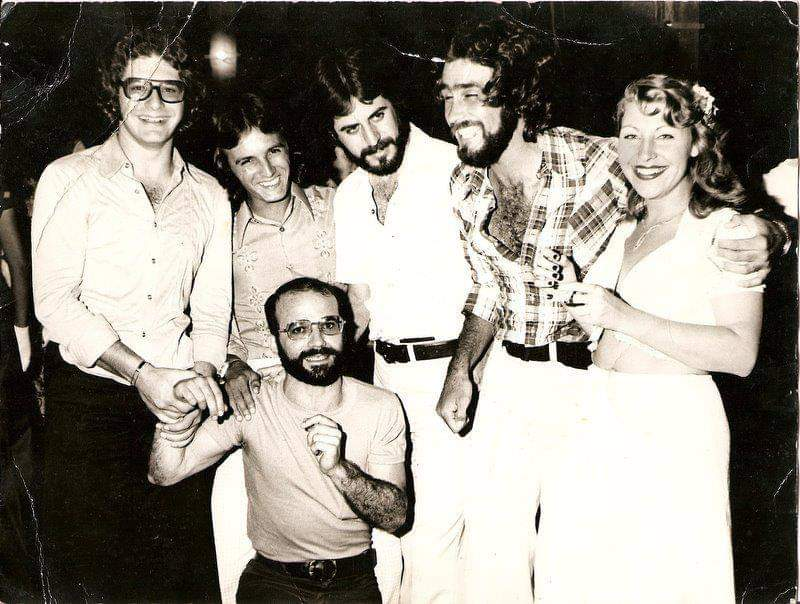
\includegraphics{Imagens/TurmaSalto.jpeg}

\textbf{Carlos Alberto, Laerte, Cláudio, Naile, Tânia e Carlinhos da
Marvina}

Claro que olhando para a foto e conhecendo seus componentes fica óbvio
que existia alguma sacanagem por trás (ou pela frente mesmo!). Afinal, o
Carlinhos não é muito grande, mas aí devia estar ajoelhado. E como todos
sabemos, ajoelhou tem que rezar!\\
A Tânia está, lindamente, representando as meninas da turma.\\
A lembrança triste revelada pela foto é a de que nosso amigo Carlos
Alberto já partiu. Deve estar rindo de alguma coisa por aí\ldots{}..

Num baile em Pilar do Sul, o Dineu do Calixtro \emph{arrodiô} o salão
inteiro tirando as moças prá dançar e levando não. Chegou num canto,
desenxavido e comentou com os colegas de baile: Narciso Martelo, Mário
Pirú, Toninho Moreira: \emph{Puta merda, vou levá um caminhão carregado
de tábua po Sarto}. Levar tábua era o supremo da humilhação: você
atravessa o salão ansioso para dançar com aquela menina bonita e leva
tábua: um sonoro não na cara. O duro é atravessar o salão de volta com
os olhares maldosos: tomou outra tábua.

O Zé do Lico trabalhava na ensacadeira de cal no forno do Aníbal de Góes
e quando arranjou uma namorada num baile em Sorocaba, falou prá moça que
trabalhava numa fábrica de talco (caprichando no ele) em Salto de
Pirapora. A mãe da moça tinha parentes por aqui e foi procurar o
pretenso futuro genro: mostraram o Zé do Lico na boca da ensacadeira
c´um pano tampando a boca por causa do \emph{puêrão} da cal. Fim do
namoro.

O Naile conversando com uma moça num baile do Sorocaba Club,
\emph{ingatô} uma prosa sobre estudo. A moça perguntou o que ele estava
estudando. Inventou que tava fazendo a quarta série no Estadão (Colégio
Estadual Júlio Prestes de Albuquerque, na Av. Eugênio Salerno). A moça
perguntou que matérias ele tinha mais dificuldade. Respondeu na bucha:
Aritimética e Linguage. Noutra oportunidade, lembrando de alguém que
falou num curso de Edificações no Liceu, tascou na lata da moça: Tô
fazendo um curso de\ldots{}\ldots{}, de\ldots{}\ldots{} (í num vinha a
mardita da palavra): Um curso de Especificações.

Outra vez num consultório na Avenida Paulista, onde tinha ido consultar
sobre a necessidade de uma cirurgia de fimose ficou com vergonha de
falar para a moça bonita da recepção o motivo da consulta, pergunta
necessária para a ficha médica e respondeu: Quero falar com o doutor. A
moça insistiu e ele mandou: É uma operação íntima.\\
Também numa rara ida a um restaurante, meteu o palito nas bolotas de
manteiga pensando que era queijo. Disse que a boca ficou \emph{iscumano}
que nem sapo, tentando disfarçar até fazer escorregar prá dentro as
bolinhas ensebadas de manteiga. A grande vantagem do Naile é que ele
mesmo nos contava essas histórias e nunca procurou esconder as bolas
fora.

O Sidnei, irmão do Naile, foi na churrascaria do Marques, na avenida São
Paulo, em Sorocaba, e no lavatório ficou esfregando a mão no vidro da
bunda da saboneteira: não percebeu que tinha que virar o vasinho de
ponta cabeça prá sair o sabão.

O Laertinho na praia disse prá mina que era carioca, todo cheio de
sotaque carioquês: Ih aí mina, qual o teu nome? Ela respondeu: Morgana.
E o Laerte: viu Morrrrrgâna carregando no érre, bem sartopiraporês. A
moça sacou no ato que a conversa era pura cascata.

Outros bailinhos de Salto tinham como damas a Ditona, a Maura do Gustão
(Viação Corneta), a Mileide do Mírto Pêxe, Jurema e Lúcia da dona
Aparecida, Noêmia, Iracema, a Cirley e as moças do Pedro Belo: as irmãs
Leda e Zelinda além da sobrinha Zélia e tantas outras.

O pessoal de Salto de Pirapora quando falava que ia a Sorocaba o pessoal
perguntava: vai comê bolinho de pêxe no mercado. Era um bolinho de
sardinha do Mercado Municipal onde ficava o ponto de ônibus de Salto.

Sorocabano então quando ia a São Paulo sempre levava o indefectível
guarda chuva pois se dizia que em São Paulo chovia direto. Você chegava
em São Paulo e falava que era de Sorocaba e ouvia: Trouxe o guarda
chuva? E a fama não era descabida não: vi muita gente usando até
galochas na capital. Uma espécie de luva de borracha impermeável que se
vestia sobre o calçado. Além do guarda chuva e a capinha de chuva
dobrada, pronta para ser acionada.

Uma vez fomos num baile em Sarapuí, acho que lotando a perua do Seu
Olézio, dirigida pelo Paulo. Lá pelas tantas, depois de muita coca cola,
o Zug foi ao banheiro\ldots{} feminino. Quando saiu da casinha onde
estava o vaso, deu de cara com duas meninas. Sem o que fazer, soltou:
que moderno, o banheiro é unisex!!!

\section{Saltopiraporices: gírias e expressões próprias e da
região}\label{saltopiraporices-guxedrias-e-expressuxf5es-pruxf3prias-e-da-regiuxe3o}

Procurei fazer um registro das gírias e maneirismos que ouvi na
convivência com pessoas de hábitos antigos e também de gírias criadas ao
acaso, muitas vezes até sem muito sentido mas, que pela repetição e
propagação no boca a boca passaram a fazer parte intrínseca do
palavreado diário e coloquial: Plagiei o título de \emph{Sorocabanices}.

\textbf{GÍRIAS PARA}

\begin{itemize}
\tightlist
\item
  \textbf{DIZER QUE ESTÁ TUDO BEM:} Num tem musquito. Conosco num tem
  enrosco. Conosco ninguém podosco. Tudo chove´s love´s positivo.
\item
  \textbf{PAQUERA:} Frestiá: A muié deu uma frestiada, eu entrei cum
  tudo.
\item
  \textbf{DINHEIRO:} -- arame, grana, farpa, carvão (essas são do Tim
  Maia, usadas no Rio de janeiro). Shintolo: Gede, vô do Rogério e
  companhia usava essa expressão. Orombongue (do \emph{dialeto} do
  Cafundó, tinha gente capaz de conversas inteiras nesse dialeto. Lembro
  do Sérginho Martelo que era craque nessa \emph{língua})
\item
  \textbf{SEM DINHEIRO:} Duro. Liso. Orombongue nâni(\emph{dialeto} do
  Cafundó).
\item
  \textbf{QUEM TÁ LIMPANDO O NARIZ:} Vai tê baile? Tá limpano o salão?
\item
  \textbf{CARA CHATO:} Minhoca fedida (horrorosa). Sór quente (quem
  aguenta ficar mais de 10 minutos no sol quente. Essa é de Sorocaba)\\
\item
  \textbf{FLATOS MAL CHEIROSOS:} Faquiáro o bode. Cachitende (cupópia do
  Cafundó). Cagáro no mundo. Soltou um foguetinho. Pisô no sapo (pelo
  barulho, ou buia).
\item
  \textbf{QUEM MORREU:} Esticô as canela. Apitô na curva. Bateu as bota.
  Viajô fora do combinado (Rolando Boldrin). Foi p´o andar de cima.
\item
  \textbf{DESIGNAR QUE ENQUADROU O SUJEITO:} Foi no figo (Mauro
  Bezerro), Foi no suan. Foi no miolo.
\item
  \textbf{DESIGNAR LOUCOS:} Tantã. Cachorro lôco. Sujeito variado das
  idéia. Doido de pedra. Maluco das idéia. Meio treze.(Curiosidade: No
  Rio de Janeiro maluco é 22)
\item
  \textbf{DESIGNAR IDIOTAS:} Pateta. Bocó de mola. Tonto. Lelé da cuca.
  Ruim das idéia. Varzeano. Por fora.
\item
  \textbf{DESIGNAR QUEM SE DEU MAL:} Saiu com uma quente e duas
  fervendo. Saiu rasgano. Saiu fedeno. Sartei de banda.
\item
  \textbf{QUEM SE DEU MAL NA VIDA, OU NAS BREGANHA (ESCAMBO, TROCA):}
  Deu o peido que o cú não aguenta. Deu o passo maior que a perna. Caiu
  do cavalo. Tomô na peida. Tomô no fiantã. Tomô no chipuco. Tomô no
  sessenta fôia. Virô um chapéu véio. Quebrado: adjetivo que se fala com
  um certo prazer. Sim, há prazer de ver as pessoas quebrarem. Mais do
  que ver o sucesso.
\item
  \textbf{DESIGNAR MULHER GOSTOSA:} Que baita chipucão. Que cachorrão.
  Que baita quadrado. Boa de carcaça. Que baita carroceria. Nhô Juca:
  Que baita muiérão, se fosse uma porca dava 8 lata de banha. Maderaima
  (Pedro Orive). Tem uma bela comissão de frente. Tem uma baita testa.
  Nos dias de chuva usa uma sombrinha para cobrir a cabeça e um
  enceradinho para cobrir a carga.\\
\item
  \textbf{SUJEITO QUE NÃO PRESTA:} Sujeito tráia. Trelento. Tranquêra.
  Curva de rio. Inrosco. Num vale déstão de mér cuado. Sê trocá por
  merda, ainda sai no lucro. Num vale o prato que come. Num vale uma
  bósta. Tranquêra.
\item
  \textbf{SUJEITO METIDO:} Come mortadela e arrota perú. Empombado.
  Metido a sebo. Seboso. Caga sebo. Tá c´o cú que é só bosta(Pedro
  Orive).
\item
  \textbf{CARAS ENJOADOS E FRESCOS:} Finório. Almofadinha. Nójento.
  Fresco. Viadinho. Bichola.
\item
  \textbf{QUEM SE ARREPENDE:} Tocô sanfona. Mijô pá tráis que nem égua.
  Deu pá tráis. Correu da ráia. Peidô, paga um cancã.
\item
  \textbf{DISTRATAR UMA PESSOA:} Tirô manã de fulano. Fez pôco caso.
  Sortô cobras e lagartos em cima de fulano. Você num vale deiz tostão
  de mér coado. Num vale a cumida que come.
\item
  \textbf{PARA PESSOAS QUE GOSTAM DE COMER OU BEBER DE GRAÇA:} Serróte.
\item
  \textbf{CORTE NO DEDO:} Deu um táio (aí pode usar pó pá tapá taio).
  Passa peida fogo (merthiolate). Feiz uma buceta no dedo. Arrancô a
  tampa do dedão. Ralô o dedo. Deu uma esfolada.
\item
  \textbf{ANIMAIS:} Boi tucura. Pé duro(gado sem raça). Cavalo
  gázio(ruim de zóio). Cavalo náfco(manco). Égua ruzia. Égua baia.
  Cavalo sarmeado (pintado). Vaca cabana (chifres baixos). Vaca varadêra
  (serve para mulher infiel também). Cavalo pampa. O cavalo tá arrastano
  os quarto. Mula manca. Égua barranquêra. Cavalo bão de andadura. Boi
  bão de caxa (carcaça).
\item
  \textbf{PESSOA PÃO DURA:} Biscoito de sordado(Dona Malvina). Munheca.
  Sovina. Mão fechada. Mão de vaca (no Rio de Janeiro se diz mão de
  porco!). Num pága nem a luiz pá dormí.
\item
  \textbf{MULHER OFERECIDA:} Lambisgóia. Biscate. Muié de vida fácil.
  Muié de rua. Mulher alpinista: trepa prá subir na vida. Guidão (deriva
  de Margaridão e do ato de segurar o guidão da moto emulando o ato
  sexual). Lambreta (corruptela da Guidão que era puta véia e as
  lambreta as puta nova).
\item
  \textbf{ZONA DO MERETRÍCIO:} Putêro, Inferninho, zona, Casa de
  Tolerância. Bordé. Currutela(Mato Grosso). Casa das quenga. Casa das
  rapariga(nordeste). Rendez-vous (casas de encontros em São Paulo e Rio
  de Janeiro).
\item
  \textbf{GÍRIAS DIVERSAS:} Só por muída.Só por bufo. Mais num machucô?
  Disguiô na carrera (perdeu o bonde da história). Só por bufo: Vamo lá
  vê a briga, só por bufo?
\item
  \textbf{DIZER QUE NÃO QUER PROSA COM O OUTRO/OUTRA:} Pode erguê a
  tanga. Pode erguê as trapêra. Pode erguê o nangs.
\item
  \textbf{SUJEITO MAL CUIDADO:} Burro de viúva: Quando o marido morre a
  viúva deixa de cuidar do animal que fica crinudo, sem casquiá (cuidar
  dos cascos). Már ajambrado. Már acabado. Torto no cabo. Gadeiuda (Dona
  Malvina). Ruim de tipo. Mindigo. Cuberto de trapo.\\
\item
  \textbf{APAIXONADOS:} Virô a cabeça por causa de fulana. Tá cuzido.
  Mandô um élis (L de lembrança). Tá de arrasto. Tá de quatro. Tá
  chorano as pitanga.
\item
  \textbf{BÊBADOS:} Tá cercano frango. Tá cum trimilique. Tá trupicano.
  Levô um trupicão. Chamô Jesus de Genésio. Enfiô o pé na jaca (o
  correto seria enfiar o pé no jacá que é quando o sujeito sai da roça
  com o milho carregado nos jacás no lombo do burro e depois de apurar o
  dinheiro da venda, toma em cachaça na venda, e volta prá roça com os
  pés dentro dos jacás vazios, dormindo em cima do lombo do burro). Vê
  que cai, deite. Verga, mais num cai.
\item
  \textbf{DIZER QUE VAI CHOVER:} Tá clamariano (calmariando:parando o
  vento). Se jeito regula, vai chovê. Tá cum revolução de chuva. Tá
  trovejano. São Pedro tá mudando os móve no céu. Mira, Diós está
  fotografando nuestra tierra (Argentinos metidos). Tá vazano gente p´o
  ladrão.
\item
  \textbf{DESIGNAR EFERVESCÊNCIA:} Tá fervido(Sorocabanice). Tá bombano.
  Tá bombaninho.\\
\item
  \textbf{A MARDITA DA ERVA:} Dar um tapa na cara da onça. Empinar pipa
  na laje. Suave na nave.\\
\item
  \textbf{COISA RUIM:} Cosaruim - assim mesmo tudo emendado e
  pronunciado rapidamente. Designa criança malvada ou sujeito ruim
  mesmo.\\
\item
  \textbf{SUJEITO DE MÁ ÍNDOLE:} Ruim de fio. Foice, enxada, maxado ou
  outra ferramenta que não está bem afiada está \emph{ruim de fio}.o
  \emph{fio} é a lâmina cortante de uma ferramenta.\\
\item
  \textbf{INDEIS:} Quando a galinha botava no mato ou na capoeira e
  quando se achava o ninho não era prudente retirar todos os ovos pois
  ela mudaria o local do ninho, dando uma \emph{trabalheira} para
  localizar o novo ninho. Retiravam-se os ovos, deixando apenas um que
  era chamado de \emph{indeis}, na verdade uma corruptela de \emph{um
  deles}. Descobri agora no fantástico Google. Outra grafia possível:
  indez.\\
\item
  \textbf{RESSALTAR QUALIDADE:} O TUFO DE BÃO -- Esse foi um
  \emph{maneirismo saltopiraporês} que nunca ouvi fora daqui. Exemplos:
  Esse carro é o tufo de bão. Esse cavalo é o tufo de bão na lida.
\end{itemize}

\textbf{EXPRESSÕES SALTOPIRAPORENCES}

\begin{itemize}
\tightlist
\item
  \textbf{FOGO DE PÁIA:} Muito usada para quem começa uma tarefa com
  muito embalo e desiste logo em seguida. O fogo de palha é fugaz e não
  tão duradouro e constante quanto o de lenhas grossas ou toras.\\
\item
  \textbf{RODÔ:} Perdeu a hora: Hoje \emph{rodei} e perdi a condução.\\
\item
  \textbf{DISGUIÔ NA CARRÊRA:} Se perdeu no caminho. A \emph{carrêra} é
  uma aposta de corrida de cavalos ou mesmo de pedestrianismo. Também
  significa falta de persistência na tarefa que se propôs a fazer.\\
\item
  \textbf{REVOLUÇÃO DE CHUVA:} Quando o tempo \emph{vira} ou quando está
  \emph{carmariano} como já explicamos.\\
\item
  \textbf{SANGRIA DISATADA:} \emph{Num percisa saí correno, num é
  sangria disatada}. A sangria é um ferimento que levou uma atadura de
  pano e se desatada pode levar à hemorragia. Ou seja precisa sair
  correndo para estancar o sangue, ou a sangria.\\
\item
  \textbf{NUM É ZÓIO DE SANTO:} Não precisa buscar a perfeição. Conta-se
  que antigamente um dos esconderijos para o dinheiro era dentro das
  estátuas sacras e esses valores eram introduzidos pelos olhos do
  santo. Assim sendo, tinham que ter um acabamento perfeito para não
  despertar desconfiança de que continham valores escondidos.\\
\item
  \textbf{A CONVERSA AINDA NÃO CHEGOU NA COZINHA:} Quando alguém dava um
  \emph{pitaco} na conversa, que não era de sua alçada se respondia
  assim emulando que a conversa da sala de estar estava restrita à mesma
  e não deveria vazar para a cozinha, leia-se para os serviçais.\\
  -\textbf{MEIO AÍVO:} Difícil até de explicar o significado e muito
  menos a origem. Quando a coisa ou o sujeito não estão muito bons.
  Fulano tá meio \emph{aÍvo} comigo. Essa mandioca tá meio \emph{aÍva}
  de gosto e assim por diante\ldots{}\\
  -\textbf{ALTO FALANTE DO VITÓRIO SKILACI:} O serviço de alto falante
  era uma coisa importante na vida da cidade pequena. Em Leme, perto de
  Ribeirão Preto, o operador/locutor tocava músicas antigas de muito bom
  gosto. Na nossa cidade o locutor era o \emph{Seu Vitório} que
  anunciava os acontecimentos sociais como nascimentos, aniversários e
  falecimentos (com a infalível marcha fúnebre). A mulher do Vitório era
  a verdadeira \emph{Dona Redonda} da novela e muito \emph{injuada}.
  Houve muita encrenca devido ao seu comportamento nada convencional
  para a pequena cidade do interior. O Vitório era um sujeito polêmico
  que queria se meter na política e também causou grandes confusões. Vou
  apurar um caso que o Castanha me contou e não consigo me lembrar
  agora.\\
  -\textbf{DÁ O TAPA E ESCONDE A MÃO:}\\
  -\textbf{QUATRO ZÓIO:} Para quem usa óculos\\
  -\textbf{CORPO DE CARRINHO DE SORVETE DA KIBON:} Para as retilíneas\\
  -\textbf{CORPITCHO DE BUJÃO DE GÁS:} Para as gordinhas\\
  -\textbf{GAMBITO:} Pernas de gambito. Para as magrelas. No
  saltopiraporês gambito é um pedaço de vara, de uns 40 centímetros que
  é usado para \emph{cochar} a corda de uma carga e estirá-la. Como é
  uma vara fina surgiu a analogia com as pernas finas das magrelas. O
  gambito na linguagem do xadrez é uma jogada em que o peão defende o
  rei.\\
  -\textbf{SACO DE OSSO:} Também para magrelas ou magrelos.\\
  -\textbf{SENTA A PUA:} Seria como \emph{manda bala}, desce o cacete.
  -\textbf{O TUFO DE BÃO:} Bom demais, supimpa.\\
  -\textbf{ZÓIO DE PORCO:}\\
  -\textbf{FOGUETÊRA VÉIA:}\\
  -\textbf{FINCA O MÚQUE:} Desce o cacete, senta a pua.\\
  -\textbf{CUM DOR NOS QUARTO:} A geração do meu pai não falava que
  tinha dor na coluna e sim usava essa expressão. A carcaça do boi é
  dividida em quartos: traseiros e dianteiros. Deve vir daí a origem.\\
  -\textbf{MALACAFENTO:} De mau aspecto, feio. Que está com malaca,
  doente. Malaca: moléstia de pele que apresenta feridas.\\
  -\textbf{PICEGO:} -- Corruptela de cego. Se diz também de quem tem um
  olho caído, meio caolho.\\
  -\textbf{CAPADÓCIO:} -- Usado no sentido pejorativo: Ignorante,
  burro.\\
  -\textbf{JAGUARA:} -- Usado para cão vira lata, gado sem raça e para
  humanos com as mesmas características.\\
  -\textbf{VIU A VIOLA EM CACO:} -- Se dizia quando a coisa \emph{ficava
  preta}, ou sendo mais politicamente correto: \emph{quando o bicho tava
  pegando}.\\
  -\textbf{CHUVA DE MANGA:} -- Para designar uma chuva passageira.
  Pensei que era de manga curta (de camisa). Na verdade é a lenda do
  Menino Mário no Chade. No conto, é uma chuva rápida que lava as folhas
  da mangueira e faz desabrochar a florada.\\
  -\textbf{JAGUAPOCA:} -- Cachorro ou gado vira lata, sem raça\\
  -\textbf{O QUÊ BODE VÉIO:} -- Dos ano 70, quando alguém contava
  bravatas ou alguma vantagem. No estilo: Tá podendo hein?\\
  -\textbf{BAMO MATÁ O BICHO? Vamos tomar uma? Seria matar o bicho da
  sede ou da vontade de beber.\\
  -}PORVA, PORVINHA:** -- Coisinha ruim, de qualidade inferior. Esse
  remédio é porvinha.\\
  -\textbf{MAIS SUJO QUE PAU DE GALINHEIRO:} -- Pessoa que tem péssima
  reputação na cidade, por motivos morais ou financeiros.\\
  -\textbf{RECURSENTO:} -- Ouvia essa expressão no futebol. Quando um
  beque despachava a bola para fora do campo era chamado assim.\\
  -\textbf{CHORANDO A MORTE DA BEZERRA:} -- Alguém se lastimando por uma
  perda amorosa, ou financeira, ou de oportunidade.\\
  -\textbf{CHUVICA DE MOIÁ BOBO:} -- Chuvica é termo da Maju da Globo
  mas \emph{chuva de moiá bobo} é saltopiraporice da gema.\\
  -\textbf{PEIXÃO, BOAZUDA, BOA DE CAXA:} -- Todas para expressar mulher
  gostosa. O boa de caxa (caixa) também é usado para gado que se presta
  à engorda.\\
  -\textbf{TOMÔ NO FIANTÃ, TOMÔ NO FUSQUETE, TOMÔ NA TOBA, TOMÔ NO
  SESSENTA FOIA, TOMÔ NA PEIDA:} -- Todas com o mesmo sentido e que
  dispensam explicação.\\
  -\textbf{PARDIAR (pardal) DISPENADO:} -- Para mulheres magrinhas, sem
  tutano, ruins de caixa.\\
  -\textbf{NUM CONTE C´O OVO NO CÚ DA GALINHA:} -- Não contar com o que
  ainda não está ao seu alcance.\\
  -\textbf{MAIS POR FORA DO QUE MINHOCA EM PEDREIRA:} --\\
  -\textbf{NOVILHA ZULEGA:} -- Azulada\\
  -\textbf{CAVALO RUZIO (ROSILHO):} -- Rosado.\\
  -\textbf{BOI TUCURA:} -- Ruim de raça.\\
  -\textbf{VACA CABANA:} -- Chifres baixos tortos para baixo.\\
  -\textbf{CAVALO NAFCO:} -- Cavalo manco ou com defeito na perna.\\
  -\textbf{VACA DE TREIS TETO:} -- Vaca ruim para produção de leite,
  defeituosa.\\
  -\textbf{GADINHO PÉ DURO:} -- o mesmo que tucura, ruim de
  raceamento.\\
  -\textbf{JAGUARA:} -- Cão ou cavalo ou gado sem raça: cachorro vira
  lata.\\
  -\textbf{MUIÉ VARADÊRA:} -- Comparação com a vaca que vara a cerca
  atrás do touro do vizinho.\\
  -\textbf{COCÊRA LAZA:} -- Para mulheres
  \ldots{}\ldots{}\ldots{}\ldots{}\ldots{} ou para pessoas inquietas,
  sem paciência de esperar.\\
  -\textbf{MUIÉ QUE COSTURA PRÁ FORA:} -- Mesmo sentido anterior.\\
  -\textbf{DEU UM NÓ EM FULANO:} -- Enganar, passar para trás, calar a
  boca ou aplicar uma sinuca de bico. -\textbf{SINUCA DE BICO:} -- No
  jogo de sinuca (snooker) quando um jogador aplica uma sinuca no
  adversário, este tem que se virar para sair da sinuca, usando as
  tabelas da mesa para atingir a bola da vez. Se não sair da sinuca
  perde o número de pontos correspondente àquela bola. Na sinuca de bico
  a bola branca é escondida no cantinho curvo da caçapa impossibilitando
  o outro jogador de fazer qualquer movimentação da bola branca.
  Traduzindo sinuca de bico é usado para definir uma situação sem saída,
  sem solução.\\
  -\textbf{DISGUIÔ NA CARRÊRA} -- Perdeu o rumo. A carrêra é a corrida
  de dois ou mais cavalos e o que disguiô na carrêra é o que \emph{negou
  fogo}, desistiu da contenda.\\
  -\textbf{PELOS DENTES SE CONHECE A IDADE DO CAVALO} -- É um fato mas
  também serve como metáfora para sujeitos falsos e dissimulados.\\
  -\textbf{RABO DE ARRÁIA} -- Ameaçando alguém de lhe dar uma
  \emph{rasteira}.\\
  -\textbf{TOMOU SOPA DE LETRINHA HOJE?} -- Quando alguém começa a falar
  palavras difíceis.\\
  -\textbf{QUANDO UM BURRO FALA, O OUTRO ABAIXA A ORELHA} -- Quando o
  interlocutor interrompe a fala de alguém.\\
  -\textbf{TÁ CUM CALOR? BATA A BUNDA NO TAMBOR}\\
  -\textbf{TÁ CUM FRIO? BATA A BUNDA NO RIO}\\
  -\textbf{CHUVA COM SÓR, CASAMENTO DE ESPANHÓR}\\
  -\textbf{TERRENO MUITO CEDENTADO} -- Os \emph{minhocas} ou seja gente
  da terra assim se referiam aos terrenos muito acidentados, difíceis
  para as práticas agrícolas como arar, gradear, semear e colher.
  Fazíamos piada sobre esses terrenos íngremes: \emph{Tem que plantá
  milho cum espingarda e coiê de laço} ou \emph{o boi pasta dis
  costa}.\\
  -\textbf{VACAGALOPORCO} -- Os nomes de três animais formavam um
  cacófato nada sugestivo.\\
  -\textbf{MEUS OLHOS POR TIÇÃO E MEU CORAÇÃO POR TIGELA} -- Abusando
  dos cacófatos.\\
  -\textbf{JOGO DO BICHO} - Deu na cabeça: dezena, centena e milhar.
  Quando o apostador do joguinho ilegal mas, disseminado amplamente,
  \emph{lavava a égua} acertando nas três possibilidades.\\
  -\textbf{BATÊ UM RANGO, FILÁ UMA BÓIA, BATÊ UMA JANTA} - Sinônimos
  para comida ou almoço ou janta.
\end{itemize}

\textbf{MARVINICES}

Dona Marvina também tinha seus \emph{ditos} e expressões peculiares!!

\begin{itemize}
\tightlist
\item
  \textbf{MEIO AÉREO:} Quando se referia à uma pessoa meio desligada,
  meio \emph{por fora}.\\
\item
  \textbf{BISCOITO DE SORDADO:} Para designar, delicadamente, o sujeito
  \emph{pão duro}. O soldado ia para a guerra e para se garantir
  guardava uns biscoitos no seu farnel. Com o tempo esses biscoitos
  ficavam muito duros e secos, daí a analogia com o pão duro.\\
\item
  \textbf{BOA BISCA:} Aquele sujeito não é boa bisca.\\
\item
  \textbf{ISPICULA MACHO:} Para meninos que viviam fazendo perguntas o
  tempo todo. Imagino que o ispicula venha de especular, indagar,
  perguntar.\\
\item
  \textbf{MEIO AÉREO:} Para sujeito desligado, por fora, ou seja que
  vive voando baixo.\\
\item
  \textbf{MIJÔ FORA DA PICHORRA:} Deu pá tráis, deu bola fora, não
  sustentou o que tinha dito.\\
\item
  \textbf{NÃO DÁ PARA TIRAR LEITE DE PEDRA:} Não dá para fazer milagres.
  O dinheiro acabou, não tem como fabricar.\\
\item
  \textbf{NUM TÁ ESCRITO NA TESTA:} Não dá para saber se a pessoa é boa
  apenas pelas aparências.\\
\item
  \textbf{MEIO AVOADA:} Meio aloprada.\\
\item
  \textbf{SÓ PÁ INGLEIS VÊ:} Está enganando, escamoteando ou seja
  fazendo bonito só para o inglês (o estrangeiro) ver.\\
\item
  \textbf{AQUELE NUM É DE MATÁ C´O A UNHA:} O cara não é fácil.\\
\item
  \textbf{MIJÔ FORA DA PICHORRA:} Deu pá tráis. Não honrou o trato. O
  mesmo que \emph{mijô pá tráis}.\\
\item
  \textbf{O ROTO FALANDO DO RASGADO:} O mesmo que o sujo falando do
  incardido.\\
\item
  \textbf{PODE AZULÁ DAQUI:} suma da minha frente.\\
\item
  \textbf{AQUELA PITOTUDA:} Quando se referia às mulheres que usavam o
  tal \emph{pitote} para manter o cabelo preso num coque em cima da
  cabeça.\\
\item
  \textbf{CANTA BEM SEM VIOLA:} Quando alguém ousava pedir algo de
  graça.\\
\item
  \textbf{FEZ DE GATO E SAPATO:} Abusou. Escarneceu. Com certeza faz
  analogia com um gato destruindo um sapato.\\
\item
  \textbf{OVO VIRADO:} Dona Malvina usava muito essa expressão quando
  alguém estava mal humorado, \emph{cabisbundo}(invenção minha) ou
  macambúzio(kkkk). A galinha quando está com esse incômodo não
  conseguia mais por ovos ,nem comer ou beber ou defecar. Ficava numa
  situação irritadiça e incômoda, daí a analogia com o mau humor dos
  humanos.\\
\item
  \textbf{GORFANDO:} Antigamente se dizia que a pessoa estava
  \emph{gumitano} ou com \emph{ânsia de gômito}. Quando a pessoa estava
  vomitando também se usava a expressão \emph{tá gorfando} ou seja
  expelindo golfadas.\\
\item
  \textbf{INTOJADA:} Num tenho paciência co´a aquela muié intojada. É um
  intojo. O intojo poderia definir a \emph{frescura} da pessoa ou por
  querer esnobar junto às pessoas.\\
\item
  \textbf{CARNE DE VACA:} O Luiz meu irmão também usava muito a
  expressão. Quando uma coisa estava ficando chata ou repetitiva diziam:
  \emph{Chi, isso tá ficando carne de vaca}. No sentido que enjoava,
  \emph{dava intojo}.\\
\item
  \textbf{ESTRONDO:} Quando estava \emph{trovejano} minha mãe dizia:
  Nossa, cada baita estrondo. Ou então: \emph{Aquilo foi um estrondo}
  quando queria dizer que alguma coisa fez sucesso ou causou impacto.\\
\item
  \textbf{TÔ VENDENDO PELO PREÇO QUE EU COMPREI:} Quando contava um
  \emph{causo} e alguém começava a duvidar da história. Aliás eu odeio
  essa postura quando conto alguma coisa e ouço: Será que é verdade? Não
  pode ser, é impossível. Costumo responder com a expressão
  \emph{malviniana} e digo que não fui e nem vou investigar nem fazer
  interrogatório aos personagens da história.\\
\item
  \textbf{A PORTA DA RUA É A SERVENTIA DA CASA:} Quando a conversa de
  uma visita não estava do seu gosto ou quando nós reclamávamos de
  alguma coisa.\\
\item
  \textbf{MANTÊGA DERRETIDA:} Quando uma criança (inclusive eu) começava
  a chorar sem motivo.
\end{itemize}

\textbf{PEDRO OURIVICES:}

O vocabulário do Pedro Orives era bem característico, peculiar e
criativo!

\begin{itemize}
\tightlist
\item
  \textbf{CAIPIRA DO RABO GROSSO:}\\
\item
  \textbf{QUEM ABAIXA DEMAIS MOSTRA A BUNDA:}\\
\item
  \textbf{TÁ INGANADO C´A COR DA CHITA:} Chita era um tecido barato
  muito usado pelas mulheres: \emph{vestido de chita}, \emph{saia de
  chita}.\\
\item
  \textbf{FEIO É ROBÁ E NUM PODÊ CARREGÁ:}\\
\item
  \textbf{SAIU C´UMA QUENTE E DUAS FERVENO:}\\
\item
  \textbf{COMEU GATO POR LEBRE:}\\
\item
  \textbf{BOBO ERA 7, MORREU 8:} Sujeito ladino.\\
\item
  \textbf{O BOI DISGUARITÔ P´O MATO:}\\
\item
  \textbf{SE JEITO REGULA, VAI CHOVÊ:}\\
\item
  \textbf{PAU DE VIRÁ TRIPA:} Suleito muito magro.\\
\item
  \textbf{FEIO É PINTO QUE NASCE PELADO:}\\
\item
  \textbf{O BOBO RALEIA, MAIS NUM FÁIA:}\\
\item
  \textbf{NUM SOCO SÓ:} Pedro Orive usava essa expressão quando ia
  movimentar um pau pesado com 3 ou mais pessoas e a expressão era no
  sentido de todo mundo fazer força, ou \emph{forcejar} no mesmo momento
  e ritmo.\\
\item
  \textbf{REGATÊRA:} Quando a égua levantava o rabo e saia em debandada
  ele dizia: Chi, essa égua tá muito regatêra hoje.\\
\item
  \textbf{BOA SIBÉRIA:} Não sei de onde meu pai tirou essa. Quando
  alguém ia viajar ou alguém \emph{de casa} estava saindo ele usava essa
  saudação. Talvez nem tivesse causa ou explicação.\\
\item
  \textbf{COLEGA DE ESCOLA:} Quando as duas éguas se davam bem, ele
  dizia: \emph{São colega de iscola}.\\
\item
  \textbf{O QUE É DE GOSTO É O REGALO DA VIDA:} No sentido que não se
  pode criticar ninguém por certos gostos.\\
\item
  \textbf{FAZENO VERÃO:} Quando estava se preparando para fazer algum
  serviço ou uma viagem a Sorocaba. Estava adiando a tarefa e dizia:
  \emph{Tô fazeno verão pá começa o serviço}.\\
\item
  \textbf{RANRULLE:} Quando ele foi para São Paulo, na estação de trem
  tinha um vendedor de jornais que anunciava em altos brados o nome do
  jornal italiano \emph{FANFULLA} da seguinte forma: Rio de Janeiro, São
  Paulo, Belo horizonte: \emph{FANFULLA} e prosseguia para a Europa:
  Lisboa, Madri, Londres: \emph{FANFULLA}. Anunciava que o vespertino
  trazia notícias do Brasil e do mundo inteiro e meu pai imitava o
  vendedor com a palavra que ele assimilou: \emph{RANRULLE}.\\
\item
  \textbf{PORCA CABANA:} meu irmão Crizólito levou o papai passear no
  Rio de Janeiro e ele voltou todo garboso contando dos lugares que ele
  conheceu inclusive a praia de \emph{PORCA CABANA}, no seu registro
  pessoal para \emph{COPACABANA.} E contava isso na barbearia e nas
  conversas e eu tive que aguentar muita gozação por conta disso mas,
  depois passei a achar muito engraçado a sua criatividade. Cabano ou
  cabana seria um boi ou vaca sem chifres então mais ainda que o sentido
  se complica.
\item
  \textbf{O VIRADO DE OVO:} o Pedro Orive era muito guloso e nas suas
  andanças nos sertões de Piedade e Ibiuna, a cavalo com seu ponche,
  chapéu, revolver Colt Cavalinho (ah como eu queria tê-lo guardado pois
  é arma de coleção) \emph{pediu poso} num conhecido na beira da
  estrada. Foi bem recebido e no dia seguinte, logo cedo foi convidado a
  se sentar à mesa para usufruir de um lauto café da manhã. No centro da
  mesa uma travessa transbordando de \emph{virado de ovo}. Para quem
  nunca comeu são ovos estalados com queijo branco e farinha de milho.
  Iguaria caipira inesquecível. Ele adorava e puxou a travessa e lotou
  um prato fundo já salivando a boca para atacar a apetitosa e fumegante
  comida. Quando deu a primeira colherada veio a surpresa: faziam o
  virado com açúcar e não com sal como ele estava acostumado. Com
  vergonha de devolver, teve que ir engolindo devagar sorvendo
  \emph{canecadas de café para fazer rodar o virado prá dentro do
  bucho}. Dona Marvina tripudiava depois: \emph{Tá vendo hóme guloso,
  tinha que inchê o prato: Bem feito}. E ele soltava sonoras
  gargalhadas.\\
\item
  \textbf{A SALA INCLINADA:} Num outro \emph{pôso} viajando com o meu
  irmão Salvador arrumaram colchões no chão para que eles dormissem na
  sala. Só que a mesma era em desnível e eles rolavam para o canto mais
  baixo da sala. Tudo virou \emph{causo} e risadas depois.\\
\item
  \textbf{DISCADERADO, C´UM DOR NOS QUARTO:} Quando ele sentia dores nas
  costas usava essas expressões. Era comum dizer que \emph{estava com
  dor nas cadeiras} ou \emph{com dor nos quarto} que na verdade denomina
  as costas do boi que tem o quarto dianteiro e o quarto traseiro.\\
\item
  \textbf{FICÔ PÁ CACHAÇO:} \emph{Sorterão encroado} como diria
  Alvarenga, da dupla com Ranchinho.\\
\item
  \textbf{FICÔ PÁ GALO CAPÃO:} No mesmo sentido da anterior.\\
\item
  \textbf{NUVIA MACHORRA:} Novilha que não pega cria.\\
\item
  \textbf{RANCOIO:} -- O porco ou boi quando tem uma \emph{capação}
  defeituosa ou seja inutiliza apenas um \emph{grão} (testículo)
  continua a dar coberturas porém não \emph{emprenha} as fêmeas; fode
  mas não cria.\\
\item
  \textbf{SUJEITO CHARQUE:} Cara chato. Deve ser porquê o charque é
  muito salgado, além de seboso.\\
\item
  \textbf{VIVA O HERME DA FONSECA:} Deve ter origem no tempo da
  revolução mas ele usava para qualquer comemoração e especialmente para
  brindar com um copo de cerveja.\\
\item
  \textbf{VAI CAGÁ ONE NUM FÊDA:} Suma daqui, não encha o saco.\\
\item
  \textbf{FOI DE ROÇÁ:} Prá dizer que foi num eito só. Servia para
  designar uma briga ou \emph{um péga prá capar}. Quando faz um serviço
  completo: \emph{Demo um péga de roçá}.\\
\item
  \textbf{PASSÔ DE RABO ERGUIDO:} Para pessoas que passavam sem
  cumprimentar. O animal que não quer ser pego na corda ergue o rabo e
  desata num \emph{carreirão}.\\
\item
  \textbf{NÃO AGUENTÔ NO PÉ DA ESTRELA:} Com certeza se referia à
  estrela da espora do cavalo ou mesmo a ponta do ferrão, com que se
  cutucava os bois de carro. Na viadagem de hoje seria considerado crime
  por molestar o animal.\\
\item
  \textbf{HOJE NUM FIZ NEM PÔ FUMO:} -- Quando não se produziu nada ou
  melhor não ganhou nem \emph{um déstão de mér cuado}.\\
\item
  \textbf{DA PRATELÊRA DE CIMA:} Para pessoas de classe mais alta, ou
  mais refinadas ou cultas.\\
\item
  \textbf{TOCÔ SANFONA:} Quando se desistia do negócio que já estava
  engatilhado.\\
\item
  \textbf{MIJÔ PÁ TRAIS:} No mesmo sentido do anterior: \emph{Mijô pá
  trais que nem égua}.\\
\item
  \textbf{TOME TENÊNCIA:} Tome jeito. Tome tento.\\
\item
  \textbf{REGULAR DO MEIO:} Quando não estava muito bom nem muito ruim.
  Para comida, trabalho ou para a qualidade de um animal.\\
\item
  \textbf{TÁ MADURANO:} Usava quando ficava apertado para correr no
  banheiro: \emph{Acuda Turca (para Dona Malvina) que tá madurano}, ou
  seja a fruta que está para cair do galho, ou de ser apanhada. Analogia
  com a merda mesmo.\\
\item
  \textbf{A TURCA LEVANTOU ESPAIANDO BRASA PÁ TUDO LADO:} Quando a Dona
  Marvina levantava brava.\\
\item
  \textbf{FORTE E RIJO?:} Uma saudação muito usada quando se encontrava
  um amigo, que há tempos não se via.\\
\item
  \textbf{INFIÔ A VIOLA NO SACO:} Saiu perdendo, saiu sem graça à moda
  de um violeiro que não agradou.\\
\item
  \textbf{NUM É DE MATÁ C´O A UNHA:} Não se mata como pulga.\\
\item
  \textbf{HOJE ELA LEVANTÔ C´O OVO VIRADO:} Quando a mulher levanta de
  mau humor, à semelhança de galinha desesperada que não consegue botar
  o ovo, porquê está virado.\\
\item
  \textbf{DOR´AMA PÔ CORPO:}\\
\item
  \textbf{TÔ DERREADO:} Tá acabado.\\
\item
  \textbf{TÔ DISINXAVIDO:} Tá sem graça.\\
\item
  \textbf{QUEM VÊ CARA NÃO VÊ CORAÇÃO:} Para pessoas falsas ou más.
\item
  \textbf{MALACAFENTO:} -- Sujeito mal ajambrado, de péssimo aspecto.
\item
  \textbf{EU SE ENFORCO NUM PÉ DE COVE:} Quando só de gozação dizia que
  preferia morrer do que passar por determinada situação.
\end{itemize}

\section{Modernices (ou não) usadas em Salto de
Pirapora}\label{modernices-ou-nuxe3o-usadas-em-salto-de-pirapora}

\begin{itemize}
\tightlist
\item
  \textbf{JACARÉ QUE DORME DE BARRIGA PRÁ CIMA VIRA BOLSA DE MADAME:}
  Autoexplicativa.\\
\item
  \textbf{X-MICO OU X-PANZÉ X-VELÓRIO:} Os dois primeiros para pão com
  banana e o último para o clássico \emph{sanduba de mortandela} dos
  velórios acompanhado de café bem doce (para enjoar logo) e fraco (para
  render).\\
\item
  \textbf{MAIS POR FORA DO QUE CEBOLA EM SALADA DE FRUTAS:}
  Autoexplicativa.\\
\item
  \textbf{CHIQUE NA BOTINA (PILAR DO SUL):} Sapato novo.\\
\item
  \textbf{MAS QUE CACHORRÃO:} Usada em São Paulo década de 50 para
  mulher boazuda. Mas as espertinhas tinham a resposta na ponta da
  língua: cachorrão sim, mas não pega viado. kkkkkk\\
\item
  \textbf{CARA DE CAPIVARA ATROPELADA:} Mulher feia.\\
\item
  \textbf{A CICLOVIA TIM MAIA (RJ) NÃO AGUENTOU A PRIMEIRA RESSACA:}
  Numa referência à ciclovia Tim Maia que desabou.
\end{itemize}

\section{\texorpdfstring{Novelices de ``O Bem Amado'', \emph{Roque
Santeiro} e
outras}{Novelices de O Bem Amado, Roque Santeiro e outras}}\label{novelices-de-o-bem-amado-roque-santeiro-e-outras}

Algumas expressões de novelas que viraram quase que Saltopiraporices!

\begin{itemize}
\tightlist
\item
  \textbf{VAMO TOMÁ UM INGASGA GATO?:} Uma cachacinha (Zeca Diabo(Lima
  Duarte)).\\
\item
  \textbf{AQUELE É UM SAFADISTA MILITANTE:} Odorico Paraguaçu(Paulo
  Gracindo).\\
\item
  \textbf{AQUELE É UM SUJEITO URUBUZENTO:} Odorico Paraguaçu.\\
\item
  \textbf{VAMOS DEIXAR OS ENTRETANTOS E PARTIR PARA OS FINALMENTE:}
  Odorico Paraguaçu, encurtando e cortando a conversa.\\
\item
  \textbf{VIVA ODORICO, MORRA ODORICO:} Nezinho do Jegue (Wilson Aguiar)
  elogiava o prefeito de Sucupira quando estava sóbrio e o vaiava quando
  estava bêbado. Metáfora sensacional que na verdade define o povo, os
  eleitores no sentido contrário. Tecem loas quando estão embebedados
  pela lábia do político sabido que acabou de assumir e depois, passado
  o \emph{embevecimento} passam a vaiar e criticar, sem dó.\\
\item
  \textbf{EU QUERO APRENDÊ A LÊ DE CARRERINHA:} Zeca Diabo querendo
  aprender a ler para fazer um curso de \emph{potrético} (protético).\\
\item
  \textbf{POSSO PENETRAR?:} Professor Astromar(Rui Rezende) pedindo
  permissão para adentrar a sala da casa do prefeito Florindo Abelha e
  da dona Pombinha. Ele ia visitar a Santinha (Lucinha Lins, linda) que
  lhe deu o fora a novela toda.\\
\item
  \textbf{VAI, PENETRA LOGO, VAI:} O prefeito Abelha(Ary Fontoura)
  autorizando a tal \emph{penetração}.\\
\item
  \textbf{É JUSTO, É MUITO JUSTO, É JUSTÍSSIMO:} Coronel Belarmino (José
  Wilker ). Conta-se que a expressão não estava no roteiro mas José
  Wiler, ao esquecer a sua fala, não se perturbou e cunhou a expressão.
  \emph{É justo} se tornou a marca registrada do Walter Benedetti,
  lendário e folclórico cidadão da nossa cidade onde quando se fala para
  o cara que ele é um sujeito justo, tem outra conotação bem diferente e
  para lá de maliciosa.\\
\item
  \textbf{Ó XENTE, MY GOD:} Dona Altiva (Eva Wilma) na novela \emph{A
  Indomada}.\\
\item
  \textbf{DEITE, QUE EU VOU LHE USAR:} Coronel Justino (José Wilker)
  quando queria ter relações com a esposa Sinhazinha (Maitê Proença) que
  acabou lhe botando os chifres com o dentista Dr Osmundo (Erick Marmo)
  mas, acabaram fuzilados em pleno ato pelo Coronel corneado.\\
\item
  \textbf{HONRA SE LAVA COM SANGUE:} Bordão e costume dos nordestinos
  corneados.\\
\item
  \textbf{VAMO BEBÊ FULANO?:} Dessa forma se homenageava o morto, em
  intermináveis rodadas de cachaça, no gargalo, madrugada adentro.\\
\item
  \textbf{TÔ CERTO OU TÔ ERRADO?:} Sinhozinho Malta, o Coronel de
  chapelão chacoalhando concomitantemente a sua grossa pulseira
  barulhenta (com o som caracterísco amplificado pelos sonoplastas.\\
\item
  \textbf{VOU AO ESTILISTA CAPILAR:} Professor Astromar indo ao
  barbeiro.
\item
  \textbf{BANDIDO FACINOROSO, CARCARÁ SANGUINOLENTO:} Sinhozinho Malta
  ao se referir a Roque Santeiro.
\end{itemize}

\section{Algumas famílias numerosas de Salto de
Pirapora}\label{algumas-famuxedlias-numerosas-de-salto-de-pirapora}

\begin{itemize}
\tightlist
\item
  \textbf{TURMA DO PEDRO ORIVE:} Francisco, Adauto, Crizólito, Luiz,
  Delphino, Maria, Horácio (depois tirou o H) e o Degas aqui, Carlinho
  da Marvina.\\
\item
  \textbf{TURMA DO FOGÃO:} Do casamento do nhô Marcílio (trabalhou na
  Incalesa) coá Nhá Aurora nasceu a \emph{renca} de filhos: Dito Fogão,
  Dáia, Martinho, Messia e Nemía, Misake, Zadi (casou com o Dito Bode),
  Davi e Elia. Nove filhos: só perdeu para o Pedro Orive e Marvina: dez
  filhos.
\item
  \textbf{TURMA DO JOÃO DA NHÁ COTA:} Ovídio, Sizina, Dorival, Balaio
  (Pedro Geraldo) e Ana, que foi casada com o maledetto João do Broco.
\item
  \textbf{TURMA DO VICENTE DA NHÁ COTA:} Era casado com a Dona Rôla,
  filha do Nhonhô de Góes e Dona Virgulina e veio a prole: Vardinho
  (casado com a Terezinha do Lindonor, minha prima), Osmar, Ademar
  (casado com a Dirce do Ditinho Mandú), Ana (casada com o Fuade), Anita
  (casada com o João Turco) e Virgulina (casada com o Zé Bode).
\item
  \textbf{TURMA DO JOÃO DO NÍSIO:} Como diria o Pedro Orive: só
  cachaços: Pracídio, Zé Antonio (Gordo), Zelão, Luizão, Glória (Antonio
  Carlos) e Fernando.
\item
  \textbf{TURMA DO VICENTINHO MARCELO E DA SIZINA DO JOÃO DE NHÁ COTA:}
  Marisa, João Vital, Zé Carlos, Júlio, Gersinho, Marilda, Mara e Bida.
\item
  \textbf{TURMA DO CABO ARLINDO E MARIA DE LOURDES FABIANO:} José, Luiz
  Fabiano, Dalvino, Ana, Sandra, Rosa, Nelson e Neusa.
\item
  \textbf{TURMA DO MÁRIO SORDADO E DONA MARIA:} Ditinho, Neifo,
  Paulinho, Maria Inês, Maria Eunice e Patrícia.
\item
  \textbf{TURMA DO MANECO (genro do Seu Manoel Português):} Benedita,
  Maria, Luiz, Ana Lúcia, Nelson, Manuel, Damaris, Luciana.
\item
  \textbf{ZÉ MARTELO E DONA CÉLIA:} Pedro Henrique, Angela, Sérgio,
  Célia, Marcos, Beto, Carlos, Nenia e Flávio.
\item
  \textbf{ROMÃOZINHO:} Renê, Vanda, Aristides, Fábio, Marlene, Sérgio e
  Nilo.
\end{itemize}

\section{Carlos Zéfiro e a barbearia do
Romãozinho}\label{carlos-zuxe9firo-e-a-barbearia-do-romuxe3ozinho}

Romãozinho, um dos maiores \emph{aumentadores de histórias} de Salto de
Pirapora, era o barbeiro titular até um certo tempo, mas foi passando o
ofício para os filhos. O único que seguiu e está até hoje na profissão é
o Renê. Quando o Renê assumiu de fato o negócio, passou a esconder
revistas pornográficas do Carlos Zéfiro debaixo da almofada da cadeira
Ferrante, para deleite de alguns e total descaso da minha parte pois
achava que na verdade os aficionados gostavam mesmo era de ver os
enormes \emph{cacetes} dos personagens. Nunca gostei do gênero muitos
menos de filmes pornográficos com a exposição exagerada da genitália de
ambos os sexos. Gosto mais de filmes com conteúdo erotizante, com poesia
e arte na linha de Lady Chaterley (veja em
Música\ldots{}\ldots{}\ldots{}e cinema ítem 2.2.13) Sempre gostei mais
da sugestão do que da exposição. A rapaziada que batia ponto na
barbearia onde o Renê tirava onda de cantor. Tinha até um bongô para
tirar um ritmo. O lugar era uma espécie de \emph{point} obrigatório
quando não se tinha o que fazer a não ser bater papo, escutar mentiras e
perscrutar as tais revistinhas escondidas embaixo da almofada. A
rapaziada ficava ensandecida e extasiada ao mesmo tempo vendo os toscos
desenhos e as pobres historinhas que tentavam criar um certo suspense
mas, serviam mesmo para exposição dos tais detalhes porquê na época a
maioria não poderia ver ao vivo tais nuances dos corpos.\\
Só por curiosidade, veja quem foi Carlos Zéfiro: Letrista. Desenhista.
Funcionário público. Como desenhista, assinava Carlos Zéfiro e foi o
responsável pelas revistinhas eróticas que embalaram os sonhos e desejos
dos jovens das décadas de 1950, 1960 e 1970, conhecidas entre os
adolescentes da época como um \emph{Catecismo básico} do sexo. Somente
no ano de 1991 é que a vida dupla de Carlos Zéfiro foi exposta pelo
jornalista Juca Kfuri, em matéria publicada na Revista Playboy, na qual
o público ficou sabendo que o autor das revistinhas era ninguém menos
que o lerista e compositor Alcides (Aguiar) Caminha. Em 1996, Marisa
Monte em seu disco \emph{Cor de Rosa e Carvão} prestou-lhe homenagem
fazendo alusão ao seu traço singular nas ilustrações pertencentes ao CD,
distribuindo no lançamento vários de seus livrinhos. No ano de 1999, a
Prefeitura Municipal da Cidade do Rio de Janeiro, em sua homenagem,
batizou com seu pseudônimo famoso, a Lona Cultural Carlos Zéfiro, no
subúrbio de Anchieta, no Rio de Janeiro. No ano de 2018 a Editora Noir
lançou a biografia \emph{O Deus da sacanagem: A vida e o tempo de Carlos
Zéfiro}, escrita pelo jornalista baiano Gonçalo Júnior. Uma de suas
belas composições, em parceria com o gênio Nelson Cavaquinho, aqui
interpretada pelo não menos gênio Paulo Moura, foi
\href{https://www.youtube.com/watch?v=fKfYOJjjOQc}{Notícia}. Outra, mais
conhecida e também maravilhosa, em parceria com Nelson Cavaquinho e
Guilerme de Brito, foi
\href{https://www.youtube.com/watch?v=l5rIRWU5rEM}{A Flor e o Espinho},
aqui numa incrível interpretação de Alexandre Pires. (texto adaptado do
Dicionário Cravo Albin da Música Popular Brasileira).

\section{Curiosidades da Região}\label{curiosidades-da-regiuxe3o}

\textbf{CAMA PATENTE SELO AZUL} -- Fabricadas na bucólica Vila Élvio em
Piedade, vizinha à nossa Salto de Pirapora. Até há pouco tempo a fábrica
era dirigida com mão de ferro pela matriarca da família. A vila
praticamente foi formada pelos funcionários da empresa, que detinha as
terras em volta da fábrica, em grande extensão. Tinham a estrutura de
ferro e molas. Mas eu conheci uma com estrutura de madeira. Se tornaram
símbolo de resistência e durabilidade. Com a modernidade dos móveis em
MDF, as tais camas caíram em desuso, sendo consideradas antiquadas. No
entanto, eu acredito que nenhuma cama tinha a durabilidade das
\emph{Patentes}. Os móveis modernos em MDF, vendidos com o simpático
nome de móveis planejados, são na verdade uma imposição do mercado que
produz móveis, já com intuito de se \emph{desfazerem} rapidamente,
estimulando as trocas e movimentando o comércio. O material MDF, que é
uma espécie de madeira prensada com resíduos, não tem durabilidade, não
aguentam serem remontadas e se houver umidade vão literalmente se
desfazer. Ou seja, em nome da modernidade os móveis de madeira maciça ou
ferro que duravam praticamente a vida toda foram desprezados e
esquecidos, mesmo com sua qualidade atestada por várias gerações. Eu
tenho absoluta certeza que muita gente passou toda a sua vida de adulto
em uma cama Patente, de solteiro ou de casal.

\textbf{CARPETE} - Outra modernidade \emph{besta} é o carpete: acumula
poeira, junta ácaros e por aí vai. Quem já viu um carpete com anos de
uso ser arrancado sabe do que estou falando. Era \emph{chique} ter uma
casa toda acarpetada. Para mim tem que ser piso de madeira \emph{cumaru}
ou \emph{ipê}. Dá trabalho para \emph{sintekar} mas o visual e a
qualidade é completamente diferente. Os defensores do modernismo como o
Zé Antonio, de Campinas, que me desculpem mas prefiro ser antiquado
nesses quesitos.

\textbf{OVNIS NO MORRO DA MARIQUINHA} -- Surgiu um boato de que no
bairro dos Morros, em Sorocaba, foram vistos OVNIS -- Objetos Voadores
Não Identificados. Na noite de 8 de janeiro de 1.979 um estudante teria
visto uma luz estranha no local e acionou a polícia que num comboio de 8
viaturas passou a noite perseguindo a tal luz e uma suposta nave
espacial. O jornal Cruzeiro do Sul estampou uma manchete relatando que
1.000 pessoas foram ver o tal objeto, mesmo com chuva. O boato cresceu e
o local virou um ponto de peregrinação por várias semanas. O
acontecimento criou o \emph{programa de caça aos OVNIs, lá pás banda do
Bairro dos Morro}. O Degas aqui esteve lá, juntamente com o Norminha,
apelido do Moisés, futuro marido da Cris do Jairo Anhaia e o Beto
Benedetti, ambos molecões na faixa de 16 ou 17 anos. O Norminha ganhou o
apelido por conta da personagem Norminha, do Jô Soares. Gostou do
apelido e cravou: \emph{My name is Norman}, todo orgulhoso pelo seu
inglês com sotaque saltopiraporês. O Beto, por sua vez, ficou por muitos
anos repetindo o bordão \emph{normaniano} cada vez que me via nas ruas
de Salto de Pirapora.

\textbf{BURACO QUENTE} - Quase ia me esquecendo da única opção para
matar a fome: o sanduíche \emph{buraco quente}, que consistia num pão
filãozinho sem miolo, que era retirado sem cortar o pão deixando um
buraco onde era colocado o recheio com carne moída e molho de tomate e
cebola. Uma delícia.

\end{document}
